%=================================================================
%				preamble
%=================================================================
\documentclass[11pt,letterpaper]{book}

\newcommand{\theauthor}{Thomas Graf}
\newcommand{\lastname}{Graf}
\newcommand{\university}{Stony Brook University}	
\newcommand{\emailaddress}{lin637@thomasgraf.net}
\newcommand{\coursenumber}{Lin 637}
\newcommand{\coursename}{Computational Linguistics 2}
\newcommand{\semester}{Spring 2016}
\newcommand{\thetitle}{\texorpdfstring{%
            {\Huge \coursename}\\
            \semester}%
            {\coursename\ [\coursenumber, \semester]}}
\newcommand{\thekeywords}{graduate level, lecture, computational linguistics, phonology, syntax}
\newcommand{\thedate}{}

\usepackage{mypackages}
\usepackage{mycommands}


%=================================================================
%			title format
%=================================================================
\author{\theauthor}
\title{\thetitle}
\date{\thedate}

%=================================================================
%			content
%=================================================================
% \includeonly{./tex/strictlylocal,./tex/sl-mathematics,./tex/sl-alternatives}

\pagestyle{empty}
\begin{document}
\maketitle
\raggedbottom
\pagenumbering{Roman}
\tableofcontents
\clearpage

\pagestyle{fancy}
\setcounter{chapter}{-1}
\chapter{Syllabus --- You Better Read it!}
\label{cha:syllabus}
\setcounter{page}{1}
\pagestyle{fancy}

\fcolorbox{gray!25}{gray!25}{%
    \centering
    \begin{tabular}{ll}
        \textbf{Course:} Computational Linguistics 2\quad\qquad\qquad&
        \textbf{Name:} Thomas Graf\\
        \textbf{Course\#:} Lin637 &
        \textbf{Email:} lin637@thomasgraf.net\\
        \textbf{Time:} TR 10:00--11:20am &
        \textbf{Office hours:} Tue 11:30--2:30pm\\
        \textbf{Location:} tba & %fixme
        \textbf{Office:} SBS N249\\
        \textbf{Course Website:} tba & %fixme
        \textbf{Personal Website:} \url{http://thomasgraf.net}
    \end{tabular}
}

\section{What This Course is About}

\rotatebox{0}{
    \footnotesize
    \begin{tikzpicture}[
    every node/.style = { draw, thick },
    every path/.style = { ->, thick },
    sug/.style = { dashed },
    req/.style = { },
    ]
    \node[fill=gray!25] (CL2) at (0,0) [align=center] {Computational Linguistics 2\\ (Lin 637)};

    % Prereqs
    \node (Phon) [above=of CL2, xshift=-8em, align=center] {Phonology 1 (Lin 522)\\
                                                                \emph{or}\\
                                                            Phonetics (Lin 523)
                                                        };
    \node (Syntax) [left=of Phon, align=center] {Syntax 1\\ (Lin 521)};
    \node (Math)   [above=of CL2, xshift=8em, align=center] {Statistics (Lin 538)\\
                                                                \emph{or}\\
                                                            Mathematical Methods (Lin 539)
                                                        };
    \node (CL1) [right=of Math, align=center] {CompLing 1\\ (Lin 537)};

    % CS branch
    \node (NLP) [below right=of CL2, xshift= 8em, align=center] {Introduction to NLP\\ (CSE 628)};
    \node (Machine) [below=of NLP, xshift=-8em, align=center]  {Machine Learning\\ (CSE 512)};
    \node (Speech)  [below=of NLP, xshift= 8em, align=center] {Speech Processing\\ (CSE 542)};
    \node (AI) [below=of Machine, align=center] {Artificial Intelligence\\ (CSE 537)};

    % Linguistics branch
    \node (CompSem) [below=of CL2, xshift=-16em, align=center] {Computational Semantics\\ (Lin 626)};
    \node (CompPhon) [below=of CompSem, align=center] {Computational Phonology\\ (Lin 627)};
    \node (CompSyn) [below=of CompPhon, align=center] {Computational Syntax\\ (Lin 628)};

    \node (Learn) [right=of CompSem, xshift=4em, align=center]  {Learnability\\ (Lin 629)};
    \node (Parse) [right=of CompPhon, xshift=4em, align=center] {Parsing and Processing\\ (Lin 630)};

    % Branches
    \draw[sug] (Syntax) |- (CL2);
    \draw[sug] (Phon) to (CL2);
    \draw[sug] (Math) to (CL2);
    \draw[req] (CL1) |- (CL2);
    \draw[req] (CL1.south -| NLP.north) -- (NLP);
    \draw[sug] (NLP) -| (Machine);
    \draw[sug] (NLP) -| (Speech);
    \draw[sug] (NLP) |- (AI);
    \draw[sug] (Learn |- CL2.south) -- (Learn); 
    \draw[sug, transform canvas={xshift=2em}] (Parse |- CL2.south) -- (Parse);
    \draw[sug] ($(CL2.south)-(6em,0)$) |- (CompSem);
    \draw[sug] ($(CL2.south)-(5em,0)$) |- (CompPhon);
    \draw[sug] ($(CL2.south)-(4em,0)$) |- (CompSyn);
\end{tikzpicture}

}

\begin{table}
    \centering
    \begin{tabular}{rlp{4.5cm}p{4.5cm}p{4cm}}
        \hline
        \hline
        \emph{Wk} & \emph{Classes} & \emph{Formal} & \emph{Linguistics} & \emph{Algorithms}\\\hline
        1         & Jan 27, 29     & What is computation? & History\\
        2         & Feb 3, 5       & Formalizing phonology & Why formalize?\\
        3         & Feb 10, 12     & Strictly local languages & Local dependencies\\
        4         & Feb 17, 19     & Subregular hierarchy & How powerful is phonology?\\
        5         & Feb 24, 26     & Regular languages & Abstractness\\
        6         & (DGFS)         & & \\
        7         & Mar 10, 12     & String transductions & SPE-OT equivalence\\
        \hline                       
        8         & (Spring Break) & & \\
        \hline                       
        9         & Mar 24, 26     & Weak Generative Capacity & $\text{Phonology} < \text{Syntax}$\\
        10        & Mar 31, Apr 2  & Tree languages & \\
        11        & Apr 7, 9       & Local tree languages & \\
        12        & (GLOW)         & & \\
        13        & Apr 21, 23     & Recognizable tree languages & \\
        14        & Apr 28, 30     & TAG and MGs & \\
        15        & May 5, 7       & Tree transductions & Reinterpreting the T-model\\
        \hline
        \hline
    \end{tabular}
\caption{Tentative course outline}
\end{table}


\section{Teaching Goals}
\begin{itemize}
    \item \textbf{General Skills}
        \begin{itemize}
            \item construct a logically sound argument
            \item evaluate the predictions and implications of an argument with respect to a given set of data
            \item compare and weigh different arguments
            \item knowledge of common logical fallacies and unsound reasoning steps
            \item disprove an empirically wrong or logically flawed argument 
            \item ability to detect and succinctly describe patterns in a given data sample
            \item understand the interplay of data and theory in the sciences
        \end{itemize}
    \item \textbf{Linguistic Skills}
        \begin{itemize}
            \item knowledge of a wide range of parts of speech
            \item familiarity with phrase structure rules
            \item writing phrase structure grammars to account for a given phenomenon
            \item lexicalizing rules
            \item a general understanding why computers still fail miserably at linguistic tasks
        \end{itemize}
    \item \textbf{What is it good for?}
        \begin{itemize}
            \item Argumentation and reasoning skills are the most important skill out there.
                People try to trick you all the time --- reasoning skills are your primary means of intellectual self-defense.
            \item Phrase structure grammars are widely used in the IT industry, e.g.\ by \emph{Xerox}, \emph{Nuance}, \emph{IBM} and \emph{Google}.
            \item Writing good grammars is difficult and an important skill in the construction of tree banks (text corpora where each sentence is annotated with syntactic structure). Tree banks are an essential tool for all areas of natural language processing by computers, e.g.\ machine translation, text generation and summarization, dialog systems and so on.
            \item Familiarity with syntactic structure and dependencies makes learning new languages easier.
        \end{itemize}
\end{itemize}


\section{Grading}
\begin{itemize}
    \item \textbf{Homework}\\
        weekly exercises and/or programming assignments; a random sample of homeworks will be collected and graded; solutions will be made available online after the due date
    \item \textbf{Readings}\\
        assigned on a weekly basis; you have to collectively write a summary for each reading in the course wiki (remember, it's a wiki, so everyone can tell from the editing history how much you contributed) 
    \item \textbf{Lecture Evaluations}\\
    \item \textbf{Presentation}\\
        everyone has to pick a research topic and present it at a workshop during finals week
\end{itemize}


\section{Policies}

\subsection{Contacting me}
\begin{itemize}
    \item Emails should be sent to lin637@thomasgraf.net to make sure they go to my high priority inbox.
        Disregarding this policy means late replies and is a sure-fire way to get on my bad side.
    \item Reply time < 24h in simple cases, possibly more if meddling with bureaucracy is involved.
    \item If you want to come to my office hours and anticipate a longer meeting, please email me so that we can set apart enough time and avoid collisions with other students.
\end{itemize}

\subsection{Attendance}
\begin{itemize}
    \item You do not have to show up for the lecture. However, asking questions and participating in discussions during class will improve your grade.
    \item Handouts and homeworks are posted on Blackboard.
\end{itemize}

\subsection{Homework}
\begin{itemize}
    \item Weekly homeworks, posted on Blackboard every Wednesday by 11:59pm
    \item Due the following Wednesday by 7pm (student office drop-off box)
    \item No late hand-ins!
    \item Homeworks must be typed up and printed!
    \item Collaboration on homework problems is encouraged as long as you write up the solutions by yourself, using your own words and examples.
        Most homework exercises will be fairly open ended, so it will be easy for us to see if you simply copied somebody's answer.
        Copying another student's solutions is considered cheating, with all the unpleasant consequences this entails.
\end{itemize}

\subsection{Special Needs \& Retaking the Course}
\begin{itemize}
    \item If you have any special needs that might impact your class performance (learning disabilities, impaired sight or hearing, etc.), please come to my office hours or contact me via mail so we can make suitable arrangements.
    \item If you already know that you'll be missing recitation or an exam due to religious holidays or other binding commitments, please send me an email with the specific dates.
    \item If you've taken this course before, I invite you to come to my office hours this week so we can identify problem areas and discuss how to address them.
\end{itemize}

\section{How to Ace This Course}

\begin{itemize}
    \item \textbf{Do the homeworks!}\\
        Do every single homework.
        Each homework is about 5\% of your grade.
        %
    \item \textbf{Chase those bonus points!}\\
        Try the challenge exercises, even if you aren't quite sure what the answer is.
        You might still get some points, and wrong answers aren't penalized.
        Similarly, take every single quiz to minimize the risk of a bad final dragging down your grade.
        %
    \item \textbf{Don't rush into things!}\\
        Read every question carefully (this goes for homeworks as well as quizzes).
        Make sure you know what it is you are asked to do.
        Whenever you feel like starting the solution, stop for a moment, paraphrase the question you think you are answering, and double check that this is indeed what the exercise is asking.
        %
    \item \textbf{Reflect on what you are doing!}\\
        Think about why certain exercises are on the homework.
        We're not trying to torture you, there is a reason for every single exercise, some important insight waiting to be discovered by you.
        Rote memorization is not enough for this course, you must understand the tools and how to use them.
        %
    \item \textbf{Collaborate!}\\
        Don't be a lone wolf, discuss the homework with your peers.
        That way, you make sure that you aren't misinterpreting the question, and by explaining your answer to others you can see whether it actually works, and why.
        But don't just copy somebody's answers.
        %
    \item \textbf{Ask for help before it's too late!}\\
        If you feel that you're falling behind, act immediately.
        Go to your TAs or come to my office hours so that we can go over the material you are struggling with.
        This is not like an introductory survey course where you can skip a session and start fresh on a new topic the week after that.
        Everything builds on the material that came before.
        Treat it like learning a foreign language, programming or calculus.
        Any knowledge gaps you have will grow at a rapid pace if you don't act fast.
\end{itemize}

\medskip
\begin{flushright}
    \begin{minipage}[b]{28em}
        \flushright
        \emph{The mind is not a vessel to be filled but a fire to be kindled.}\\
        Plutarch\\

        \medskip
        \emph{Learning is exploring.}\\
        Yours truly
    \end{minipage}
\end{flushright}

\pagenumbering{arabic}

\chapter{Computation(al) linguistics}
\label{cha:Formal}

Perhaps the most unfortunate fact about the field of computational linguistics is that its name is \emph{computational linguistics}.
The term inherits a dichotomy that is hard to tease apart for the uninitiated: the distinction between computers and computing.

When the layperson hears the term \emph{computational}, they immediately think of doing things with computers.
The actual hardware might be a laptop, a phone, or the NSA's giant server farm in Utah, but in the end it always boils down to some kind of electronic device that was deliberately designed and engineered by humans.
In the case of language, there certainly is no shortage of tasks we want these devices to handle: word completion for text messages, speech recognition and speech synthesis for our GPS, detecting spam mails, translating websites on the fly, and much more.
Thanks to decades of research in computational linguistics, computers now do surprisingly well at these tasks.
Sure, the existing solutions are far from perfect and occasionally make bewildering mistakes unlike anything even a highly inebriated human would produce.
The more linguistically complex the task, the worse computers tend to fare.
But the technology has proven good enough to become an essential part of our daily lives, and it keeps improving at a rapid rate.
Computational linguistics as the study and design of language technology has been a resounding success.

But language technology isn't all there is to computational linguistics.
Limiting the notion of computation to ``doing things with computers'' is doing it a great disservice.
The scope of computational linguistics goes far beyond computers.
It encompasses any object that is capable of computing, be it computers, the human brain, or abstract computing devices like the Turing machine, which isn't tied to a specific physical medium.
With this general notion of computing, the goal is no longer to solve language-related tasks.
No, \textbf{language is the task}: what does language look like from a computational perspective?

% This probably sounds rather vague to, but it is not without merit.
% Much like a physicist seeks a deeper understanding of the laws of the universe and thus opens up the road towards new technologies, the computational study of language can help with the more grounded concerns of making computers language-savvy.

The book you are holding in your hands (and, presumably, reading) is all about this broader notion of computational linguistics.
For lack of a better term, I call this \emph{computation linguistics}.
Its focus on understanding language makes computation linguistics a subfield of linguistics, even if its methods borrow heavily from theoretical computer science and mathematics (formal language theory, learnability, algebra, lattices, parsing theory, and so on).
The remainder of this chapter sharpens the profile of computation linguistics and how it differs from other varieties of computational linguistics.
I will also discuss why this approach is worth pursuing.
The specific merits of computation linguistics depends a lot on whether you are a natural language engineer, a theoretical linguist, or a cognitive scientist.
But rest assured, each group stands to gain something.

One more remark: given its subject matter, this chapter is necessarily very meta-theoretic.
If you would rather get right into the thicket of things, feel free to jump ahead to the next few chapters and come back later.
A general sales pitch for computation linguistics is all nice and dandy, but the proof of the pudding is in the eating.


\section{Computers vs computation}
\label{sec:formal_computation}

While computers are the most common tool for carrying out computations nowadays, they are not what computation is about.
Computation, in its barest form, is the principled manipulation of information, of transforming some input into some output in a precise, step-wise fashion.
When a computer verifies $1 + 1 = 2$, this act of computation is instantiated via a series of electrical impulses that affect some of the millions of transistors that make up its hardware.
But the computation is not tied to that specific electrical process, it can take many physical instantiations in this world.

The movie buffs among you will remember the 1990s masterpiece \emph{MacGyver: Lost Treasure of Atlantis}.
In this spiritual successor to the \emph{Indiana Jones} movies, MacGyver discovers the secret of Atlantis: a giant, steam-powered computer that operates without electricity.
MacGyver is incredulous --- how could they have a computer without electricity?
But the idea of a steam-powered computer is actually far from outlandish.
Any device that can assume multiple different states and switch between those states in a controlled fashion is capable of computation.

The idea that the act of computation is about transitioning from one internal configuration to another in a principled fashion is the central insight behind the \emph{Turing machine}.
% The Turing machine is named after Alan Turing (1912--1954), arguably one of the most brilliant and influential thinkers of the 20th century.
% It is impossible to do Turing justice in a few sentences, so reading up on his many accomplishments is left as an exercise to the reader.
It was first defined by Alan Turing in 1936 in his seminal paper \emph{On Computable Numbers, with an Application to the Entscheidungsproblem}.
(To the select few readers whose German is a little rusty: \emph{Entscheidungsproblem} means \emph{decision problem}).
If you understand how the Turing machine works, then you know why computation isn't tied to a specific hardware instantiation, be it electricity, steam, or the human brain.
So let us take a closer look at the Turing machine.

\begin{person}[1912--1954]{Alan Turing}
Alan Turing was an English mathematician and polymath.
His gamut of accomplishments have made him one of the most influential researchers of the 20th century.
\begin{wrapfigure}{r}{0pt}
    \includegraphics[width=8em]{./img/pic/turing}
\end{wrapfigure}
He laid large parts of the foundation of modern computer science, in particular artificial intelligence and the theory of computation.
During World War 2, he took a leading role in cracking the Enigma, an encryption device used by the Nazis.
It has been estimated that this breakthrough saved millions of lives.
Turing was also an excellent long-distance runner, and was even a contender for a spot on the British Olympic team in 1948.

Turing's numerous accomplishments were not fully acknowledged during his lifetime, and as a homosexual he even faced criminal prosecution.
In 1952, he was sentenced to undergo chemical castration treatment due to acts of ``gross indecency'' (i.e.~homosexual relations).
Two years later he died of cyanide poisoning, presumably a suicide.

Turing's dead body was found next to a half-eaten apple.
For this reason, it has been rumored that the original, rainbow-colored Apple logo is a tribute to Alan Turing and his tragic death due to the British prosecution of homosexuals.
However, Apple co-founder Steve Wozniak has called this an urban legend.
\end{person}

The Turing machine is now widely considered to establish a firm upper bound on what can be computed in a mechanical fashion.
This is astounding considering that a Turing machine consists of only three components:
%
\begin{enumerate}
    \item a tape that acts as a rewritable and infinitely extendable data storage, and
    \item a read/write head that can modify the tape, and
    \item a state register that controls the behavior of the machine.
\end{enumerate}
%
The tape is a linear arrangement of cells, and each cell stores at most one symbol.
The read/write head can move to any cell on the tape, read the symbol in that cell, and possibly overwrite it with a new symbol.
The state register is like a knob that can be in one of finitely many positions, e.g.\ 7 out of 10 on a volume dial.
Based on the symbol that is currently under the read/write head and the state of the register, the Turing machine consecutively executes three specific operations: 
%
\begin{enumerate}
    \item a \emph{write action} (overwrite or do nothing), and
    \item a \emph{move action} (move left, move right, stay in place), and
    \item a \emph{state register change} (keep state, switch to different state).
\end{enumerate}
%
A simple instruction of a Turing machine may read ``if the symbol under the head is 1 and the state is A, overwrite 1 with 0, move left, and switch to state B''.
A finite collection of such instructions is a program that can be run on a Turing machine to carry out specific computations.
% Careful, the key word here is \emph{finite}.
% Throughout this book, we will encounter various computing devices that differ widely in their power.
% And most of the time, those differences in power stem from requirements that some specific resource be finitely bounded.
% In the case of the Turing machine, the state register and the list of instructions .
% The tape, on the other hand,

\begin{examplebox}[Copying with a Turing machine]
    The table below describes a small program for a Turing machine.
    %
    \begin{center}
        \begin{tabular}{rl@{\hspace{2em}}ccc}
            \emph{current state} & \emph{tape symbol} & \emph{write action} & \emph{move action} & \emph{new state}\\
            \hline
            A            & 0                  & none                & none               & F\\
            A            & 1                  & write(0)            & $\Leftarrow$       & B\\
            B            & 0                  & none                & $\Leftarrow$       & C\\
            B            & 1                  & none                & $\Leftarrow$       & B\\
            C            & 0                  & write(1)            & $\Rightarrow$      & D\\
            C            & 1                  & none                & $\Leftarrow$       & C\\
            D            & 0                  & none                & $\Rightarrow$      & E\\
            D            & 1                  & none                & $\Rightarrow$      & D\\
            E            & 0                  & write(1)            & $\Leftarrow$       & A\\
            E            & 1                  & none                & $\Rightarrow$      & E\\
        \end{tabular}
    \end{center}
    % 
    This looks fairly cryptic, so let us tease apart what is going on here.

    The machine has 6 different states: A, B, C, D, E, and F\@.
    Only two kinds of symbols are used on the tape, 0 and 1.
    A command like write(1) means that the machine fills the current cell on the tape with a 1, whereas the arrows $\Leftarrow$ and $\Rightarrow$ specify that the machine moves one cell to the left or one cell to the right after the write action is finished.
    So line 5, for example, tells us that if the machine is in state C and has a 0 under its read/write head, it writes a 1, moves to the next symbol to the right, and switches into state D.

    That's terrific, but what is that good for?
    What does the program do?
    So far this feels like a badly written instruction manual where each individual sentence makes sense but you can't figure out how they fit together (very much \textbf{un}like this book, I hope).
    Let us boost our understanding of the program by working through a concrete example.

    Suppose that the machine starts in the following configuration: 
    The tape consists mostly of 0s, except for two adjacent 1s, and the read-write head is positioned on the rightmost 1, with the state register in state A.
    This is visualized below.
    %
    \begin{center}
        \tikzload{turing1}
    \end{center}
    %
    This configuration is matched by the second line of the instruction table.
    Hence the machine overwrites the current symbol with a 0, moves to the left and switches into state B\@.
    Here is the resulting configuration, with the changed symbol highlighted in \textbf{boldface}.
    %
    \begin{center}
        \tikzload{turing2}
    \end{center}
    %
    Since the read/write head is now over a 1 while the machine is in state B, the instruction on line 4 is triggered: the machine keeps the current symbol as is, moves to the left, and keeps the register in state B\@.
    No change is made to the tape.
    %
    \begin{center}
        \tikzload{turing3}
    \end{center}
    %
    This new configuration triggers the third instruction, which tells the machine not to perform any write action, move one symbol to the left, and switch the register to state C\@. 
    %
    \begin{center}
        \tikzload{turing4}
    \end{center}
    %
    The rest of the computation then proceeds as depicted below, which changes to the tape once again highlighted in boldface:
    %
    \begin{center}
        \tikzload{turing5}

        \tikzload{turing6}

        \tikzload{turing7}

        \tikzload{turing8}

        \tikzload{turing9}

        \tikzload{turing10}

        \tikzload{turing11}

        \tikzload{turing12}

        \tikzload{turing13}

        \tikzload{turing14}

        \tikzload{turing15}

        \tikzload{turing16}
    \end{center}
    % 
    The F state is special because it does not trigger any new instructions, so the machine halts once it reaches this state.

    Looking at the final outcome of the individual steps, we can now make sense of the instructions at the beginning of this example.
    Put together, they program the Turing machine so that it copies sequences of 1s.
    If the tape had contained 11111 instead of 11, the final output would have contained two instances of 11111.
    That's longer than the tape in our example, but remember that the tape of a Turing machine can always be extended as necessary.
    \label{ex:Formal_turingmachine}
\end{examplebox}

The example above shows that a Turing machine can create copies of an input.
As we will see in later chapters, copying is actually a very complex task that plays an important role in natural languages.
% fixme: chapter reference
Despite the complexity of copying, it can be understood in the very general terms of a Turing machine as simply a sequence of configuration changes: what does the tape look like, where are we on the tape, and what state is the machine in?

The generality of the Turing machine is what enables a broader understanding of computation that does not care about the actual hardware.
A Turing machine is not a concrete object, it's not a tiny box with some tape and a state dial that you can order from Amazon.
Instead, it is an abstract model of what it means to carry out a computation, and there are many different ways a Turing machine can be instantiated in the real world.
This is particularly noteworthy because Turing machines act as a kind of standard model for computation.
If there is no limit on how much tape is available, any problem that can be solved computationally can be solved by a Turing machine.
So all kinds of computation can be regarded as a specific program that runs on a Turing machine.
But this also means that any machine, system, or construct that provides the equivalent of a tape and a controllable read-write head is a computing device.

For example, a Turing machine can even take the form of a very selfish drinking game:
Gather 4 friends of yours and 6 shot glasses --- I am boldly assuming that you have enough of both.
Put the shot glasses in a line and fill the rightmost two with a beverage of your choice.
Then give each one of your friends a card with instructions they have to follow.
For the sake of exposition, let's assume that your friends are called Bill, Cathy, Damian, and Edith.
Their respective cards read as follows:
%
\begin{itemize}
    \item \textbf{Bill}\\
        If the shotglass in front of you is empty, get out of line and put Cathy in front of the glass to the left.
        Otherwise, leave the glass alone (sorry!), and move to the glass to the left.

    \item \textbf{Cathy}\\
        If the shotglass in front of you is empty, fill it up, get out of line, and put Damian in front of the glass to the right.
        Otherwise, leave the glass alone (sorry!),  and move to the glass to the left.

    \item \textbf{Damian}\\
        If the shotglass in front of you is empty, get out of line and put Edith in front of the glass to the right.
        Otherwise, move to the glass to the right.

    \item \textbf{Edith}\\
        If the shotglass in front of you is empty, fill it up, get out of line, and put me in front of the glass to the left.
        Otherwise, move to the glass to the right.
\end{itemize}
%
The instructions for yourself are slightly more fun.
If the glass in front of you is full, drink it all, get out of line, and put Bill in front of the glass to the left.
If the glass is empty, the game is over.

I suppose you can already tell what is going on here.
When you play this game, it will proceed exactly like the Turing machine from our copying example (it is a selfish drinking game because you are the only one who gets to drink, i.e.~rewrite a 1 as a 0).
Even though you and your friends are separate individuals, the combination of you, your friends, and the shotglasses constitutes a Turing machine.
The instructions you give each person are parts of the program that runs on this Turing machine.

We can make all kinds of changes to this setup without losing the connection to Turing machines.
For example, we may use bowls instead of glasses, and fill them with M\&Ms instead of some beverage.
And maybe we do not actually put the bowls in a line but instead assume that they all differ in size, like a set of baking bowls that is randomly distributed around your ktichen.
We then reinterpret ``left'' so that it means ``the largest bowl that is smaller than the current bowl''.
And ``right'' now means ``the smallest bowl that is bigger than the current bowl''.
Even though we no longer have the bowls in a line, we can still move ``left'' and ``right'' based on the relative size of the bowls.
Perhaps we could even replace your friends with a very well-trained dog.
Clearly a dog and a human are two very different things, but it changes nothing about the computation that is being carried out.
No matter how we set things up, the same input will always be transformed into the same output.
Shot glasses, bowls, M\&Ms, humans, dogs, it does not matter, we always end up copying the input.

Silly as these examples may be, the central point stands: making changes to the physical make-up of the device that carries out the computation does not entail making changes to the computation itself.
The notion of computation operates at a higher level of abstraction, and that is what gives it such a unifying power.
We can take computational concepts and apply them to systems that do not at all look like the computers we are familiar with: the human brain, the biological mechanisms of gene expression, even the universe itself.
Despite the differences in physical substrates, structural changes, and sheer computing speed, they are all equally valid examples of computing devices and we can  discover interesting things about them by adopting this perspective.

Hopefully you can now appreciate why it is unfortunate that the term \emph{computational linguistics} does not clearly disambiguate between computation and computers.
% \Note{At least it is better than the German term \emph{Computerlinguistik}, which can only have the second meaning when interpreted compositionally.}
While the latter emphasizes engineering concerns, the former strives for a more abstract perspective that applies to computers as well as humans.
Remember, humans are the only known computing device with perfect command of natural language.
In the spirit of learning from nature, we would do well to study language at a level that is compatible with these devices and learn from them as much as possible.

To clearly differentiate the two notions of computational linguistics, I will use \emph{natural language processing} (NLP) in this book to refer to those aspects of computational linguistics that are solely concerned with computers.
NLP is about solving language-related tasks with computers, e.g.~speech synthesis, machine translation, or even the basic search function in your text editor.
Computation linguistics is about studying language as an instance of computation.
Both NLP and computation linguistics belong to the larger field of computational linguistics, but they differ in their goals and in their methods.

% Parental advisory: a beverage with high alcohol content may cause premature failure of the experiment.
% The same computation will look very different when executed by a human brain, with neurons firing in a specific cascade that gives rise to a three-dimensional activation pattern.
% Or maybe we are just dealing with a few beads being moved around in an abacus.

While the terminology might be less vague now, the underlying concepts are still very abstract and intangible.
To some extent things will only get clearer once we move on from the high-level perspective in this chapter and start looking at concrete issues.
Still, if the road ahead is shrouded in mystery, it would at least be nice to why it is a road worth travelling.
So let us next consider why one would want to study language from a computational perspective. %, and how one might go about this.


\section{Why computation linguistics?}
\label{sec:formal_arguments}

The focus on computation linguistics might seem peculiar to you.
NLP has an easy sales pitch: ``Make the world a better place while earning a six digit salary.''
Computation linguistics, on the other hand, has less tangible goals.
Even if you are a heavily theory-minded researcher, it might not be immediately clear what computation linguistics has to offer.
But there are good arguments for computation linguistics, and they range from real-world applications to scientific insights.

\subsection{Practical arguments}
\label{ssec:formal_arguments_practical}

\subsubsection{The standard argument, and its standard counterargument}
\label{sub:formal_arguments_practical_standard}

Let us first look at an argument that seems plausible, but ends up running into several issues.
% It seems fairly easy to make a case for the importance of studying computational aspects of language (putting aside for now what exactly we mean by that). 
The argument starts with the reasonable assumption that a world in which computers can successfully handle all kinds of language-related tasks is preferable to one where they cannot.
This would create a second industrial revolution that boldly pushes automation into language-heavy domains: customer service and speech-driven user interfaces, language and writing instruction, knowledge aggregation, and much more.
Admittedly there is also the risk of mass surveillance, mass unemployment, and the social upheavals that tend to follow both, but let's assume that those would just be short-term growing pains on the way to a more prosperous future.
If this is correct, then it is imperative that we do whatever we can to get computers to this level of aptitude.
And just like some understanding of physics had to be in place before engineers could bless mankind with the radio or the combustion engine, we cannot have successful NLP applications without a minimum understanding of language and the computational challenges it poses.
Computation linguistics thus is a prerequisite for NLP\@.

This argument is intuitively pleasing and, in my humble estimate, ultimately correct.
In the form presented above, though, it is too simplistic and easy prey to somebody playing devil's advocate.
Let's take a careful look at the counterargument such a person might put forward:

One of the most shocking aspects of the applied sciences and engineering is how little genuine understanding one needs to construct a useful tool.
To give but a few examples: relativity theory is not an integral part of calculating artillery ballistics, the smallpox vaccine did not need a theory of germs, and you don't need to understand convection to build a good chimney.
In many areas of life, the permitted margin of error is large enough that shortcuts, hacks, and brute force methods will get the job done just fine.
For practical purposes it is also perfectly fine to make stipulations that fly in the face of scientific consensus but improve the final results.
In the words of Noam Chomsky, the founding father of modern linguistics \citep[147]{Chomsky90}:

\begin{fancyquote}
    Throughout history, those who built bridges or designed airplanes often had to make explicit assumptions that went beyond the understanding of the basic sciences.
\end{fancyquote}

Similar things can be observed in NLP\@.
Many of its tools and techniques ignore linguistic ideas for the sake of simplicity and efficiency.
These tools do surprisingly well and often outperform competing models that draw from what linguists have learned about language.
The state of affairs is summarized very succinctly by a hyperbolic quote that is commonly attributed to the computational linguist Frederick Jelinek:

\begin{fancyquote}
    Every time I fire a linguist, the performance of the speech recognizer goes up.
\end{fancyquote}

\begin{person}[1932--2010]{Frederick Jelinek}
Frederick Jelinek played a key role in bringing information theory and probabilistic methods to computational linguistics, or rather, bringing them back from the dead.

\begin{wrapfigure}{r}{0pt}
    \includegraphics[width=8em]{./img/pic/jelinek}
\end{wrapfigure}
Following the success of Chomsky's \emph{Transformational grammar} in the 50s and 60s, computational linguists put their hope in rule-based approaches and largely stayed away from statistics and probabilities.
Jelinek bucked this trend.
After he joined IBM in the 70s, he worked tirelessly on designing speech recognition systems that were sufficiently robust for real-world application.
The more theoretically minded, rule-based approaches had nothing comparable to offer.
By the 1990s, the probabilistic models Jelinek pioneered had become a corner stone of NLP, and they remain important to this day.
But perhaps the pendulum has swung a bit too far --- the rule-based side may still come back with a revolution of its own.
\end{person}

There are numerous examples of simple (or downright simplistic) models matching or even outperforming more sophisticated models that are deeply steeped in theory.
Consider the case of a 2013 study that evaluated various text-based models for predicting the success of novels.
Naively, one would expect that a novel's success is largely dependent on its writing style, narrative structure, and subject matter.
Yet one of the best models completely ignored those aspects and focused exclusively on word frequencies.
As it turns out, successful novels have an unusually high frequency of thought-oriented verbs like \emph{recognize} and \emph{remember}.
A model that only pays attention to such word frequency effects performs better than one that also analyzes the minute structural intricacies that linguists care about.

It seems, then, that there is a shockingly large gap between ``language as a computational problem'' and ``computers solving natural language tasks''.
The latter is doing just fine without the former, and in some cases theory may even make things worse for practical applications.

With the rapid rise of machine learning methods in recent years, one might even expect the gap to widen over the next few decades.
General purpose machine learning strategies have made major inroads in recent years, in particular in the form of neural networks.
The approaches deliberately forego all linguistic knowledge and instead opt for treating language as an arbitrary data-crunching problem like any other.
And once again they turned out to be surprisingly performant.
If this trend continues to its logical extreme, NLP may be completely absorbed into the field of machine learning in the near future.
In this case, any language-specific insights would be even harder to incorporate given the domain-agnostic nature of the machine learning techniques.
If ``computers solving natural language tasks'' simply turns into ``computers solving tasks'', then ``language as a computational problem'' might be too specific an enterprise to make many worthwhile contributions.
In sum, then, computation linguistics might have few actual contributions to make to NLP\@.

And thus we have arrived at the conclusion of the devil's advocate: while in principle computation linguists might be able to help with practical applications, recent history tells us otherwise.
Other fields like physics and chemistry might show a trickle-down effect from theory to applications, but a look at the field right now reveals no comparable pipeline from computation linguistics to NLP.

\subsubsection{A counterargument to the counterargument}
\label{sub:formal_arguments_practical_counter}

There is more than a grain of truth to the devil's advocate's reasoning, but at the same it is too narrow and overly reductionist.
Things simply aren't that black-and-white, and a more nuanced analysis reveals interesting shades of gray.

Admittedly some areas of application do not stand to profit much from linguistic insight.
For example, a government may want to improve the mental well-being of its citizens by screening tweets for signs of mental illness and offering preventive care to users that seem to be at risk.
The nature of this task is largely independent of the complexities of natural language and its computational intricacies.
For one thing, tweets are often short enough that their intended meaning can be inferred just from a few keywords and hashtags.
Second, the correlation between mental health and language use is fairly loose and not particularly well-understood.
In the absence of a robust theory, the best approach is trial-and-error: identify a few reasonable indicators of mental illness, build several probabilistic models that pay attention to these indicators, and go with the model that performs best.
This route is guaranteed to produce some kind of model within a short amount of time, and the model is very likely to perform better than any model that builds on the most recent scientific research, simply because the problem is too limited for the theoretical underpinning to pay off in a significant manner.
The more specific and restricted the problem, the less need there is for deep understanding.

But not all problems are simple or very restricted, and this leaves room for computation linguistics to make worthwhile contributions.
Language technology is still very much about going for the low-hanging fruit.
Many interesting problems remain untackled.
No computer currently understands instructions like the following: ``Go to my pictures folder and rename the files. I want each filename to start with the date and then list all the names of the people in the picture.''
A simple request, it seems, but it is actually bursting with linguistic complexity:
%
\begin{enumerate}
    \item ``my pictures folder'':
            Which folder is that?
            Who is speaking here?
            What if there's multiple folders with pictures?
            Can we make a reasonable guess about which folder the user has in mind?
    \item ``rename the files'':
            What files?
            Presumably the user only wants to rename the files in the pictures folder, not all the files on the hard drive.
            But this piece of information needs to be inferred, it is not given explicitly.
    \item ``I want'':
            So the computer should make sure that the files end up looking like what the user has in mind, even though the user isn't explicitly issuing a command.
    \item ``each filename'':
            Actually the user wants only image files like JPGs or PNGs to be renamed, whereas the PDF that they randomly dropped in there should be left alone.
    \item ``start with the date'':
            Dates can be formatted in various ways.
            Can we make a reasonable guess about what format the user wants?
            If not, how can we ask for clarification?
    \item ``then list'':
            Is this still part of the description of the filename or a new command to the computer?
            That is to say, should the filename include the names of people, or should the computer list their names for the user after each successful file renaming?
    \item ``list all the names of the people in the picture'':
            What is the intended interpretation here?
            People that appear in the picture should have their name listed in the filename?
            Each person should have their name listed in the picture?
            List every name that belongs to a group of people and appears in the picture?
    \item ``the picture'':
            Which picture?
            Probably the one that is being renamed, but again this restriction is left implicit.
\end{enumerate}
%
In our amazement that computers seem to accomplish super-human feats such as translating a website in a split-second, we tend to forget that they still struggle with language-related tasks that even a 5-year old would solve with ease.
Once one broadens the horizon from what NLP is currently working on to what NLP could be working on, the importance of computation linguistics becomes much more apparent.

In a certain sense this holds even if one considers only those areas where NLP has been successful.
Machine translation, for example, has made tremendous leaps in the last 10 years and can produce remarkable results now --- if one picks the right source and target language.
Translating a text from English to Spanish will work much better than translating the very same text from Swahili to Inuktitut.
This is because modern NLP techniques are tremendously data-hungry.
In order for a probabilistic model to perform well, it has to be fed millions of data points.
Only a few languages have enough digitized text to meet the data hunger of these models, all other languages are considered \emph{resource poor}.
Such resource poor languages are second-class citizens in the realm of NLP\@.
Note that even languages like Swedish and Afrikaans, which are spoken in very affluent countries, are resource-poor for NLP purposes.
And the problem isn't limited to languages, every dialect that deviates to a significant extent from the standard is resource poor.
So Scottish English, Bavarian German, and African-American Vernacular English are all ill-served by current NLP solutions compared to their standard counterparts.
As language technology becomes increasingly important, there is a real danger that current NLP techniques end up indirectly discriminating against (linguistic) minorities.

That this does not need to be the case is proved thousands of times each day all over the world.
Each day, children in linguistic communities of all shapes and sizes effortlessly acquire their native language from very limited input.
In fact, children are amazing language learners and frequently generalize in ways that go far beyond what the data provides.
This is what linguists call the \emph{poverty of stimulus}: even though the linguistic input children get is very limited, they infer a lot more from it than would be possible just via raw statistics. 
How exactly children manage to do this is still very much an open issue, in particular on the computational level.
But the more our knowledge advances on this front, the less data our models will need, thereby shrinking the gap between resource-poor and resource-rich languages.

It is also worth noting that the performance of NLP models should not be taken at face value because it is based on a particular notion of performance.
The NLP community has devised numerous quantitative metrics for benchmarking its models.
But these benchmarks have several blind spots in their design.
For one thing, they only measure how many errors a model makes, rather than how grave the errors are.
Suppose you have to evaluate how well two children --- let's call them Shorty and Luna --- have mastered basic addition.
The table below shows your questions and their respective answers.
%
\begin{center}
    \begin{tabular}{rcc}
        \toprule
        \textbf{Question} & \textbf{Shorty} & \textbf{Luna}\\
        \midrule
        What is 3+4? & 6 & 7\\
        What is 6+3? & 9 & 9\\
        What is 7+3? & 10 & 10\\
        What is 3+4+3? & 9 & 343\\
        \bottomrule
    \end{tabular}
\end{center}
%
Looking purely at the number of correct answers, Luna does better than Shorty.
But every teacher will tell you that Shorty has a better grasp of addition than Luna.
Yes, Shorty is short by 1 when adding up 3 and 4.
But once you take that mistake into account, all the other answers make sense.
In particular, under Shorty's mistaken assumption that $3 + 4 = 6$, it is necessarily the case that $3 + 4 + 3 = 6 + 3 = 9$.
Luna, on the other hand, missed this important generalization and gives a very puzzling answer to the last question.
Instead of adding, Luna suddenly concatenates the numbers.
That is extremely bewildering, and a teacher who only evaluates students based on how many answers they get wrong would miss this.

You might object that the problem here isn't with counting the number of mistakes, but rather with the small number of questions we asked.
If we had asked more questions of the form $3 + 4 + 3$, Luna would have done worse than Shorty.
You are correct, and this is also the answer you will hear in NLP.
NLP models are tested on millions of sentences, which the example above obviously does not do justice to.
But the size of a test sample isn't a solid indicator of its quality.
What if Luna's problem only occurs with sequences of addition of the form $n + (n + 1) + n$?
Even in a test set with millions of questions, this pattern might be fairly rare, whereas Shorty's problem with adding $3$ and $4$ might crop over and over again.
With addition it is fairly easy to design a balanced test set, but with language NLP engineers rely largely on the data that is freely available in the wild.
This includes tweets, posts on message boards, news paper articles, and so on.
Linguists have argued for a long time that these samples are not representative of the richness of language.
The most intricate aspects of language tend to reveal themselves only rarely, but when they do they are of great importance.

As a result, NLP performance metrics should be taken with a grain of salt.
Yes, model A might outperform model B by 10 points in your benchmark.
But model B might still make a better impression on users because its errors aren't nearly as serious or puzzling as those made by model A\@.
When interacting with humans, slightly wrong beats really wrong, and wrong beats weird.

Such qualitative performance metrics are still sorely missing in NLP.
A good theoretical grounding --- where ``theory'' subsumes both theoretical linguistics and the theory of computation --- is a guide through those areas of language where data is insufficient.
The more language-like a model, the less data it should need to display language-like behavior.

In sum, then, NLP approaches still have their fair share of shortcomings that insights from computation linguistics can help address.
As NLP moves into increasingly complex domains of language, with increasingly impoverished data, the use of a strong theoretical foundation will become increasingly apparent.


\subsubsection{An example from the history of computational linguistics}
\label{sub:formal_arguments_practical_history}

You might still be skeptical.
All I have done is point out some shortcomings of the current NLP approaches that could potentially benefit from computation linguistics.
I still owe you a concrete example of a fruitful transfer of knowledge.
Fair enough, so here we go:

Consider the problem of word structure, which linguists call \emph{morphology}.
A native speaker of English knows that \emph{liked} is the combination of the verb \emph{like} and a past tense marker, and in the other direction he or she also knows that the addition of a past tense marker turns \emph{walk} into \emph{walked}, \emph{run} into \emph{ran}, and \emph{go} into \emph{went}.
Linguists have collected a detailed inventory of morphological processes, and computational linguists have developed the framework of \emph{finite-state morphology} to model these processes. 
% Two-level morphology, in turn, was grounded in the theory of finite-state machines, which are a staple of computer science.
These two steps did not take place independently of each other.
The crucial contribution of linguists was to point out that the range of possible morphological processes is very limited.
Once computational linguists saw what is (im)possible in morphology, they realized that almost all the processes are very simple and can be captured with very restricted tools that are still very flexible and scalable, which is exactly what one wants for practical purposes.
Nowadays, finite-state machinery is still used for modeling specific aspects of morphology, e.g.~number systems.
This is a domain where good data is scarce and mistakes can have severe consequences --- there's a big difference between transferring \$23.45 and \$2,345.
The linguistic insights have undergone a voyage from theoretical linguistics to computation linguists to NLP, where they have proven tremendously useful for over 30 years now.
But insights have also traveled in the other direction.
A few processes in morphology that involve copying pose serious challenges to finite-state morphology, highlighting the need for a better linguistic understanding of these phenomena.
This way theoretical and computational linguists feed each other's research, with NLP as the happy consumer of the final results.

% Admittedly not all examples work out as nicely as the one above.
% In many cases the insights of computation linguistics tend to be grounded in pure math rather than linguistic fieldwork or analysis.
Sometimes the transmission of insights is almost imperceptibly indirect, and is easily lost in the fog of history.
Formal language theory --- which is an integral part of computation linguistics but also indispensable for the design of programming languages and file standards like XML --- grew out of Noam Chomsky's linguistic theories of natural language.
Chomsky's Transformational grammar also served as an important inspiration for William Rounds's work on tree transducers, and those are now used in machine translation and compiler design, the latter being indispensable for modern programming languages.
The computational linguist Aravind Joshi relied on key insights about the nature of language when he developed \emph{Tree Adjoining Grammars} (TAG), which then found applications in modeling biochemical structures such as messenger RNA\@.
The formalism of \emph{Combinatory Categorial Grammar}, which is equally driven by engineering concerns and pure linguistic theory, has been used in studying the structure of music.
As you can see, there is no telling how fields will cross-fertilize each other as their ideas and insights slowly transgress disciplinary boundaries.
But there are concrete cases of such exchange between computational linguistics and numerous other fields, including NLP\@.

\subsubsection{Interim Summary}
\label{sub:formal_arguments_practical_summary}

In sum, NLP is no different from other fields in that it, too, can profit from more theoretically minded endeavors.
This holds whether the theory is grounded in mathematics, computer science, or linguistics, each one of them has already made valuable contributions and will continue to do so.
The value of theory is not constant across all applications.
Hard problems tend to benefit more than easy ones.
It also depends on the quantity and quality of available data, and the need for strong safeties --- minor mistranslations are acceptable for a blog post, but not in a business contract.
But it is also important that the problem is well-defined.
If it isn't even clear what exactly the problem is, theory will be of very limited use.
This is why Twitter-based mental health assessment requires a healthy dose of opportunistic trial-and-error with all available tools, whereas computational morphology benefits a lot from a good theoretical foundation.
So, no, computation linguistics isn't the magic bullet for solving all of NLP's woes, but it has valuable contributions to make in key areas.
These key areas may well become the central focus of attention soon.
If the current staples of NLP end up being subsumed by general purpose machine learning techniques, we may see the field move towards harder problems that are ripe with language-specific issues.

\subsection{Scientific arguments}
\label{ssec:formal_arguments_science}

The previous section defends computation linguistics in terms of its utility for NLP\@. 
These utilitarian arguments are needed to convince politicians, taxpayers, and engineers.
But they hold no sway in the court of science.
A linguist might shrug at the arguments above on a good day and publicly denounce us as nimrods on a bad one.
If computation linguistics can somehow get NLP to incorporate more linguistic insights, that's nice.
It probably won't tell us much about language, though.
So it won't improve linguistics, psychology or cognitive science.
Fortunately, the scientific merit of computation linguistics is a lot more clear-cut than the utilitarian argument: since language is intrinsically a computational problem, studying language from a computationally informed perspective is only natural.

Neurolinguistics and psycholinguistics have already uncovered a lot about the computational side of language, whereas linguists have a lot to say about the rules and representations that make up a speaker's knowledge of their language.
Integrating the two, however, has proven very difficult for a variety of reasons.
Computation linguists provides a bridge to sythesize these diverging perspectives on language into a unified picture.

% \Note{Semantics is noteworthy for being the one subfield of linguistics that is still very strongly aligned with the externalist view of language and does not think of its formalism as the high-level description of a specific part of human cognition.
% For a mentalist approach to natural language meaning see \citet{Pietroski14}.
% }

\subsubsection{Competence and performance}
\label{sub:formal_arguments_science_competence-performance}

In order to make the argument for computation linguistics, we first have to put in place the distinction between \textbf{competence} and \textbf{performance}.
Probably the most important development in 20\tsp{th} century linguistics is the \emph{cognitive turn}, the shift from viewing language as a disembodied system of rules and words to its reinterpretation as one of humans' many cognitive abilities.
Language is not an abstract platonic object that exists independent of reality.
It is done by humans, it is an algorithm that runs on the hardware of the human brain.
Since the brain is pretty moist and mushy, its hardware is often called the \emph{wetware} to emphasize the contrast to man-made machines.
Specific languages are just specific externalizations of this abstract program ``language'' that runs on the wetware.
Languages are but a window into a specific kind of computation that the human brain carries out with little effort.
Since the cognitive turn, theoretical linguistics is no longer about languages, it is about language.

But if language is a computation carried out by wetware, this immediately raises the question how exactly language is computed.
Linguists actually split this up into two subquestions:
%
\begin{description}
    \item[Competence]
        What is the specification of the computations?
    \item[Performance]
        How is this specification implemented and used?
\end{description}
%
Competence questions are concerned with the rules of grammar and how they are encoded.
A native speaker of English, for instance, recognizes that in the two sentences below, only the first one is ambiguous.
%
\begin{exe}
    \ex
    \begin{xlist}
        \ex Who do you want to leave?
        \ex Who do you wanna leave?
    \end{xlist}
\end{exe}
%
The first question has two meanings, paraphrased as ``Who is such that you want them to leave?'' and ``Who is such that you want to leave them?'', respectively.
The second question only allows the latter interpretation.
Competence describes the implicit knowledge of a speaker that is needed for him or her to recognize such a contrast.
But the actual process of bringing competence to bear on these questions is a much more involved matter.
That's what performance is about.
% When you hear those questions in a bar, how do you filter out all the background noise, how do you break up the sound waves into words, how do you hold them in memory, how do you find all the possible readings given the rules of English, and how do you know which interpretation is the intended one?
% Those are all interesting questions, but they are beyond competence.
% They are what performance is about.
% It involves reading the questions, assigning them specific structures, and mapping these structures to interpretations.

Intuitively, we may think of a speaker's competence as a book that records the rules and laws of their language.
Those rules might look slightly different from other speakers --- even when two speakers share the same language, they often have very minor differences in what sentences they consider well-formed, which words they use, and so on.
But that is not the key point here.
What matters is that a book of law, by itself, does not do anything.
We need a law enforcement mechanism, a system for analyzing things in the real world, putting them in relation to those laws, and acting accordingly.
In the real world that's judges, police, but also the law-abiding citizen that modulates their own behavior according to the laws they are aware of.
That is the metaphorical counterpart to linguistic performance.

With language, performance takes on many facets:
analyzing the incoming sound waves,
filtering out irrelevant background noise,
breaking down the continuous waveforms into discrete chunks of vowels and consonants, 
assembling sounds into words, 
combining words into sentences,
interpreting the sentence,
marshalling sufficient working memory to store all this information,
constructing a reply,
meticulously controlling the articulatory apparatus to utter the intended reply without any mispronunciations or slips of the tongue,
and much more.
Performance is a huge chunk of language, and yet it can be very insightful to factor it out and focus only on competence.

Some linguists do not like the idea of factoring out performance, they consider competence too much of an abstraction.
Among other things, a competence-view of language implies that we have to look at language modulo any processing restrictions of the human brain, e.g.~limits on working memory and attention span.
Of course nothing of this sort can be observed in nature.
You can't have human language without the human brain, and that mushy, three pound lump is constantly subject to very tight limits on working memory and attention.
So there is no way of directly observing competence, every piece of linguistic data is the compound result of both competence and performance.

But something like the competence-performance split is actually very common in many other fields, including computer science.
Here is a concrete example.
When UPS was looking for the most efficient system to ship a package from A to B, they did not care if their solution would still work well if they had to be able to ship to 50 trillion different cities. 
That is irrelevant because Earth doesn't even have that many cities, so the issue simply would not arrive in practice.
Their problem space is bounded in size.
Yet there is a whole branch of computer science, called \textbf{complexity theory}, which studies how hard certain problems are to solve if one assumes that there is upper bound on the size of the problem.
For instance, how hard is it to sort a list if there is no upper bound on how long that list can be.
In practice, this does not matter because a computer's memory is limited, which puts a hard upper bound on the length of lists it can work with (that's in contrast to a Turing machine, where we assumed that we never run out of tape).
So why would computer scientists study a problem that can never arise in the real world?
The answer is that these unbounded problems are often more insightful than the bounded ones.
The abstraction from a bounded problem to an unbounded problem makes it clearer what the challenging parts are and how they could be optimized.
We will actually see this at various points throughout this book.
As counter-intuitive as it may seem, you often have to abstract away from reality in order to get closer to reality.

Just like computer science has benefited from looking at problems of unbounded size, linguists have learned a lot about language by factoring out performance and focusing on competence.
But the competence level is rarely viewed through a computational lens, even though language, by virtue of being a cognitive ability, is intrinsically tied to computation.
Research into how language is computed usually limits itself to the realm of performance, approaching the issue from the perspective of neuroscience and psychology: how does the wetware behave when carrying out specific linguistic tasks, and can we design a procedure that mimics humans' behavior?

For example, native speakers of English usually have no problem understanding English sentences, it is an incredibly fast and effortless process.
But it does exhibit surprising quirks.
When asked whether the sentence \eqref{ex:Formal_GardenPath} is grammatically correct, native speakers usually say no.
%
\begin{exe}
        \ex The player tossed a frisbee smiled.\label{ex:Formal_GardenPath}
\end{exe}
%
However, the sentence is actually well-formed, it has the same structure as the minimally different \eqref{ex:Formal_Non-GardenPath}. 
%
\begin{exe}
    \ex The player thrown a frisbee smiled.\label{ex:Formal_Non-GardenPath}
\end{exe}
%
For some reason the algorithm native speakers of English use has no problem with \eqref{ex:Formal_Non-GardenPath} but is thrown off track in \eqref{ex:Formal_GardenPath} which differs in only a single word that serves exactly the same grammatical function.
This is almost like a computer that can compute $1 + 2$ but not $2 + 1$.
There is no obvious reason for this behavior, and it doesn't exactly look like good engineering (so much for Intelligent Design).
Linguists have come up with various elaborate explanations of such phenomena over the years --- some more successful than others ---
but they all share a variety of properties that necessarily limit their scope and thus the questions they can address.
Where the reach of these approaches ends, the realm of computation linguistics begins.

\subsubsection{Neuroscience}
\label{sub:formal_arguments_science_neuro}

Neuroscience has made tremendous progress in the last few decades, and as a result there has also been increased interest in neurolinguistics.
As in many other areas of neuroscience, the hope is that the ``code'' of the human brain will reveal itself through its wetware.
Know the hardware, and you'll know the software; unfortunately, things are not that straight-forward.

It is certainly interesting to see how the human brain works on the hardware level.
But it is far from obvious that this tells us much about the actual computations.
Nothing we have learned about computation since Turing's pioneering work supports this notion, intuitive as it might be.
Studying a computer's hardware tells us little about what it is computing.
Suppose your computer still has an old rotary hard drive, rather than an SSD\@.
When we hear your hard drive spin up, we can reasonably assume that some file is being accessed, but that is about all we can deduce with our own senses.
Inquisitive minds that we are, we may then decide to connect a set of thermal diodes to various points of the hardware in order to detect whether this or that piece of hardware starts heating up.
Increased heat output would suggest an increase of computational activity in that specific area.
A hot graphics chip, for instance, would be indicative of some high graphical load.
But that is still very inconclusive, for various reasons.

First of all, a higher load on the graphics chip might indicate that some kind of 3D graphics is being rendered, e.g.~for a video game.
Actually, though, a lot of non-graphical tasks are outsourced from the processor to the graphics chip nowadays.
This is why the acronym GPU, which stands for \emph{Graphics Processing Unit}, has been extended to GPGPU, which is short for \emph{General Purpose Computing on GPUs}.
Among other things, GPUs are now commonly used in machine learning tasks.
Content-wise, this has very little to do with graphics rendering, but the mathematics are actually fairly similar.
This is one reason why it is difficult to draw conclusions from hardware to software --- two very different domains A and B can instantiate very similar computational problems, so that a device that looks like it is computing A might actually be computing B\@.

A curious example of this principle is the first-person shooter \emph{Doom}, well-known for its high-adrenaline gameplay and impressive music.
When this classic video game was ported from PC to Atari's \emph{Jaguar} console, buyers and reviewers alike lamented the lack of any in-game music.
The reason for that is surprising and insightful at the same time.
At the time, Doom was a very demanding game, too demanding for the Atari Jaguar.
Its CPU simply wasn't beefy enough to handle the game.
The developers, however, realized that some of the game functions could be off-loaded to another chip, freeing up more CPU cycles for the rest of the game.
But this meant that this other chip could no longer serve its intended purpose as it was busy with other computations.
Yes, you guessed it, that chip's standard role was to handle the music. 
There was no other chip with free computing cycles for the music, and thus the music had to be completely cut from the port.
While ultimately unsatisfying for Atari Jaguar owners, the developers' decision to co-opt a music chip for general purpose computation was genius.

Something similar has actually been observed in humans, where the visual cortex of a blind person will be partially co-opted for auditory computations.
Admittedly the human brain is not as content-agnostic as a modern computer, and overall specific tasks seem to be tied to specific areas of the brain.
But there is at least some flexiblity, and it is too early to say how tight this link actually is from a computational perspective.
Suppose task X is localized in brain area A\@.
Then a computationally similar task Y may or may not be localized to area A\@, there is no way of telling in advance.
In the other direction, not every task Z that is localized to A is necessarily computationally comparable to X\@.
There is no strict implication in either direction.
The locus of computation does not tell us much about the nature of computation.

There is also a severe granularity mismatch between hardware and computation that makes it very hard to make meaningful inferences from the former to the latter.
This argument was made very forcefully by Jonas and Kording in 2017.
They started with a plausible assumption: if current neuroscience techniques can tell us something about computation, then they should be able to tell us something about the computations carried out in a computer.
If we take a computer, give it a specific task to run, and collect measurements that are comparable to what neuroscientists have collected for the human brain, we should be able to detect reflexes of the computations in the data.
As you might imagine, this did not work well at all.
\citet[1]{JonasKording17} concluded that ``current analytic approaches in neuroscience may fall short of producing meaningful understanding of neural systems''.
If the hardware level can't give us conclusive evidence about the computations in a device we have perfect knowledge of, it is doubtful that the human brain can be figured out by just studying its hardware.

This basic point become downright trivial if we look at a concrete example.
Consider the simple task of searching through a list.
Suppose, for instance, that you ask somebody to memorize the list A, C, D, F, G, X\@.
Then you ask them if the list contained the symbol G\@.
How could they answer your question?
I honestly don't know how a human does it, nor does anybody else.
It can be accomplished in various ways, each with their own advantages and disadvantages, but the two most fundamental strategies are \emph{linear search} and \emph{binary search}.
%
\begin{examplebox}[Linear search and binary search]
    Suppose that our list is A, C, D, F, G, X and we want to know if G is in the list.

    Using the linear search algorithm, we simply scan the list from left to right and check one symbol after the other.
    If we find the symbol we are looking for, we reply that it is in the list.
    If we make it through the whole list without ever seeing the requested symbol, we give a negative reply.
    The table below shows what happens at each step of the computation when searching for G in the list A,C, D, F, G, X\@.
    %
    \begin{center}
        \begin{tabular}{rcl}
            \toprule
            \textbf{Step} & \textbf{Symbol} & \textbf{Remaining list}\\
            \midrule
            0 &   & A, C, D, F, G, X\\
            1 & A & C, D, F, G, X\\
            2 & C & D, F, G, X\\
            3 & D & F, G, X\\
            4 & F & G, X\\
            5 & G & done\\
            \bottomrule
        \end{tabular}
    \end{center}
    %
    As you can see, linear search finds the requested item in 5 steps.

    Binary search is a more efficient search strategy that exploits a specific property of the list.
    While in principle the symbols in a list can appear in any random order, our list A, C, D, F, G, X lists the symbols in alphabetical order.
    This fact can be used to avoid searching through irrelevant parts of the list.

    Instead of starting at the beginning of the list, binary search goes straight to the middle.
    If the middle point is the symbol we are looking for, we stop there.
    If the symbol there is alphabetically \textbf{before} the searched symbol, then we throw away the \textbf{left} half of the list.
    After all, if the middle symbol alphabetically precedes the symbol we are looking for, then so do all the symbols to the left of the middle symbol.
    Hence it makes no sense to search there.
    After the left half has been removed, we perform binary search on the remainder, i.e.~the right half.
    On the other hand, if the symbol at the middle point is alphabetically \textbf{after} the search symbol, then we throw away the \textbf{right} half of the list and perform binary search on the remainder, i.e.~the left half.
    We continue this way, throwing away one half in each step and looking at the middle point of the remaining half.
    If the list contains the item we are looking for, we will find it eventually.
    If at some point we have thrown away the whole list, the item wasn't in the list.
    %
    \begin{center}
        \begin{tabular}{rcl}
            \toprule
            \textbf{Step} & \textbf{Symbol} & \textbf{Remaining list}\\
            \midrule
            0 &   & A, C, D, F, G, X\\
            1 & D & F, G, X\\
            2 & G & done\\
            \bottomrule
        \end{tabular}
    \end{center}
    
    Binary search can be much faster than linear search.
    The further to the right in a list an item occurs, the longer linear search will take compared to binary search.
    That's because binary search can skip large chunks of the list.
    But crucially this only works if we have a guarantee that the list is ordered in a specific way --- otherwise, we can't tell which half of the list can be ignored at any given point.
    \label{ex:formal_search}
\end{examplebox}
%
On average, binary search is much faster than linear search for sorted lists.
So if we had two computers with exactly the same hardware, one using linear search and the other binary search, the latter would show vastly superior performance in general.
Yet the behavior cannot be explained in terms of hardware, because we know for a fact that the two machines are exactly the same.
This is why good algorithms and data structures are so important in computer science --- progress on the hardware side cannot match the massive speed-ups of smart software.
The ingenuity of the human brain probably does not lie in its hardware, at least not exclusively.
It stands to reason that millions of years of evolution have resulted in algorithms that have been tweaked, tuned, and optimized to be as efficient as possible for their respective domain.
Hardware alone is not enough, the true magic happens at the software level, which does not reveal itself transparently via hardware.

Keep in mind that in the case of computers, we have the additional advantage that we already know how their architecture works because we designed it.
So if that still is not enough to deduce from the hardware what kind of computations a computer is carrying out, it seems rather unlikely that a similar process could derive from wetware the functioning of the human brain.
Granted, we can uncover limiting factors and some basic facts, just like a close analysis of a processor can reveal a maximum limit on its memory and that all information is encoded in a categorical fashion via series of on and off states --- the proverbial 0s and 1s.
But all the probing, all the high-tech machinery tells us very little about the actual computations.

Thus it isn't exactly surprising that no neuroscientist on this planet knows whether at least some computations carried out by the wetware of the human brain involve anything resembling linear search or binary search.
But this is one of the simplest distinctions that can be made when it comes to search.
Many of the concepts discussed in this book are much more abstract, which makes it even harder to bridge the gap between the hardware\slash wetware-level and computation.
A strict bottom-up approach that figures out the human mind solely based on wetware is unlikely to succeed.

In the domain of language, we have the potential for a bidirectional approach that proceeds both top-down (from computation to hardware) and bottom-up (from hardware to computation).
Computation linguistics can contribute towards such a linking theory by identifying computational core mechanisms of language that are sufficiently general that they may be detectable in the wetware with current day techniques.
Computation linguistics is the glue that links fine-grained theories of competence to computational concepts that are sufficiently broad to possibly have some detectable reflexes at the hardware\slash wetware level.


\subsubsection{Psychology}
\label{sub:formal_arguments_science_psych}

In contrast to neuroscientists, psychologists don't investigate the physical instantiation of cognition.
They are perfectly happy to treat the brain's wetware as a black box that produces a certain output (= reaction) given a certain input (= stimulus).
Their goal is to develop models that replicate these input-output mappings.
But again there are certain limitations that computation linguistics can help address.

One central issue is again a granularity mismatch between the explanandum --- language as a cognitive ability --- and the means of explanation.
Psycholinguistic models can be highly specific in what cognitive parameters they presuppose.
%
\begin{examplebox}[A psycholinguistic account of priming]
    A common assumption in the literature is that humans use \emph{content addressable memory} (CAM).
    CAM operates very differently from a computer's \emph{random accessible memory} (RAM).
    RAM is similar to a very long street where one can instantaneously travel to any house as long as one knows its house number.
    So if a computer has stored some item in memory at a given address, all one needs is this address to immediately retrieve the item from memory.
    Information stored in CAM, on the other hand, is not retrieved via an address that specifies its precise location in memory.
    Instead, the individual pieces of the information themselves act as a way of specifying the path to its location in memory.
    Imagine traversing a large, maze-like network of intersecting roads, where every road has a descriptive title such as \emph{doctor}, \emph{crab}, and \emph{cartoon}. 
    At the point where those three roads intersect, you will find the house of Doctor John A.~Zoidberg, the alien crab doctor from the cartoon show \emph{Futurama}.
    There is no longer a need for arbitrary addresses because the properties of any given thing carve out the path for finding this thing.
    Psycholinguists couple CAM with certain models of memory activation and retrieval to explain specific aspects of human cognition, e.g.~that memory retrieval for item X takes less time if a content-related item Y already had to be retrieved immediately before (this is known as \emph{priming}).
\end{examplebox}
%
A very extreme case of psychologists and psycholinguists making highly specific assumptions is the ACT-R framework.
ACT-R provides an elaborate computer model of human cognition.
The specificity of ACT-R allows researcher to run detailed simulations and tweak parameters to find the best fit for experimental data.
ACT-R is an impressive achievement, but it is a machine with many knobs, cogs and gears.
This makes it difficult to ascertain what each component contributes to the final result.
This has two downsides.
First, the findings aren't as insightful as one might hope.
Simulations may tell us that configuration X accounts for the facts, but what about X$'$ or X$''$?
Do we need all the components interacting in this specific manner, or are most assumptions dispensable except for maybe one or two?

You may think that we can answer this by just running additional simulations with other parameter values.
But this is often not practically feasible due to combinatorial explosion.
If your model has 10 binary parameters, then there are $2^{10} = 1024$ different instantiations of the model.
Even if your simulation takes only half an hour to complete, you're already looking at $512$ hours, which is over three weeks.
In practice, your model will take longer to run and have many more parameters to tweak, so exhaustive simulation of all options isn't feasible.
Computation linguistics, on the other hand, has the advantage that its concepts, albeit abstract, are sufficiently simple to be explored from a mathematical perspective using little more than pen and paper.
While this certainly poses its own challenges, it often takes much less time and effort than designing models and running simulations.

Putting aside the time investment factor, we are still left with the problem that one cannot generalize from modeling results in a monotonic fashion.
That model M captures phenomenon P does not entail that it also accounts for phenomenon P$'$.
Once we make tweaks to account for P$'$, we have to rerun our simulations for P to ensure that everything still works as desired.
The mathematical approach favored by computation linguistics, on the other hand, provides crucial clues under which conditions key properties are preserved, and this makes it easier to make inferences from P to P$'$.

This is not to say that the modeling approach is inferior.
It has the major advantage that it is close to the empirical realities.
The models are complex, but their behavior and predictions can be directly tested against the observed data.
The highly abstracted and idealized concepts of computation linguistics require more effort to bring to bear on the data.
Some problems are so complex that it is far from obvious how they should be idealized in order to make them amenable to mathematical investigation.
Just as with neuroscience, this isn't a case of one approach supplanting the other, but rather of natural complementation.

Some psycholinguists may object, though, that the previous paragraphs only engage with a particular subpart of their field, namely the cognitive modeling approach.
Even if one grants that all the postulated shortcomings are on the mark, that would only apply to a small part of psycholinguistics.
The overwhelming majority of psycholinguists operates with less specific models and theories.
These models may be too coarse for computational simulations, but they work just fine as a generator of new research questions that can be explored through experiments.
While correct, these models face the opposite problem of lacking the fine-grained details that would make them sensitive to issues of linguistic competence and theoretical linguistics.
They cannot distinguish between competing analyses or illuminate whether language is rule-based or constraint-based.
Computation linguistics provides the scaffolding to explore these issues and identity properties that might be detectable in psycholinguistic experiments.

% So what does computational linguistics have to offer to the experimentalists?
%
% The answer is surprisingly simple: just like psycholinguistic proposals, computational analyses can motivate new experiments.
% The computational lens allows us to classify linguistic dependencies according to their complexity, which naturally prompts the question how this notion of complexity maps to cognitive load for humans.
% % fixme: weak point, it never works like that
%
% more neutral terms and proving in formal terms how much a model can be altered without breaking this crucial dependency.
% This also makes it easier to identify which parts of a model are truly indispensable.
% For psycholinguists, then, the central promise of computational linguistics is a theory of model classes that reduces indeterminacy and disentangles the essential from the dispensable.
%
% The lack of conclusive proof for psycholinguistic assumptions is not too much of an issue, uncertainty is a given in almost every scientific endeavor.
% One cannot help but wonder, though, if the degree of uncertainty could be lowered.
% If there is a higher-level explanation that does not rely on quite as specific assumptions about working memory, that should be preferable.
% The same goes for the problem of too many solutions: if it is possible to change the value of parameter P in a model and still get the same result as long as one also changes parameter Q, what might really matter is not P and Q as such but the more abstract dependency between them.
% The different psychological models would then be but a few of many, possibly infinitely many different ways of encoding this dependency.



\subsubsection{Interim summary: The promise of computation linguistics}
\label{sub:formal_arguments_science_summary}

The limitations of neuroscience and psychology pointed out above can be traced back to a comparatively low degree of abstraction.
Both fields operate at levels that specify a lot of information --- like memory addressing and neural connections --- whose relevance to language isn't apparent; in particular if one cares mostly about competence questions, as most theoretical linguists do.
The great promise of computation linguistics, the one advantage that sets it apart from neuroscience and psychology, is one of \emph{productive abstraction}.
Computation linguistics can completely abstract away from all extraneous detail and performance aspects without losing the connection to cognition.
The methods used by computation linguists allow us to connect language and computation (and hence cognition) at the competence level. 
We can tackle questions such as
%
\begin{itemize}
    \item What is the weakest memory architecture that is sufficiently powerful to support a specific model of competence?
    \item What is the weakest competence model that is sufficiently powerful for a given empirical domain, e.g.\ morphology.
    \item Do alternative competence models describe the same class of computations?
    \item Is there an alternative representation of a given model that lowers memory requirements?
    \item How can we carve up complex models into simple subparts? 
    \item What kind of computational universals hold of language?
          That is to say, what kind of computational properties hold of every natural language?
\end{itemize}

\section{The virtue of abstractness}
\label{sec:formal_abstractness}

\subsection{Marr's three levels of analysis}
\label{ssec:formal_abstracness_marr}

The preceding observations regarding abstractness are far from new.
In 1976, David Marr and Tomaso Poggio formulated the \emph{Tri-Level Hypothesis} in their paper \emph{From Understanding Computation to Understanding Neural Circuitry}.
They proposed that computational processes, including cognition, should be described on three levels of increasing abstraction:
%
\begin{description}
    \item[physical] the wetware or hardware instantiation; e.g.\ neural circuitry for vision or the machine code running on your computer
    \item[algorithmic] what kind of computational steps does the system carry out and in which order, what are its data structures and how are they manipulated; many aspects of programming deal with issues at this level
    \item[computational] what problem space does the system operate on, how are the solutions specified (but not necessarily carried out)
\end{description}
%
\begin{examplebox}[Set intersection on three levels]
    Suppose you have two sets of objects, $A$ and $B$, and you want to write a computer program that tells you which objects belong to both sets.
    \begin{itemize}
        \item On a computational level, that program is easily specified: it takes two sets as input and returns their intersection ($A \cap B$ in mathematical notation).
        \item On the algorithmic level, things get trickier.
        For instance, do you want to store the sets as lists or something else, and just how does one actually construct an object that is the intersection of two sets?
    \item On the physical level, finally, things are so complicated that it is nigh impossible to tell what exactly is being computed.
        In your laptop, voltages increase or decrease in various transistors spread over the CPU, memory and mainboard, and that's about all you can make out.
        In the human brain, neurons are firing in intricate patterns that somehow give rise to the desired output.
        Unless you already have a good idea of the higher levels and the computational process being carried out, it is probably hopeless to reverse engineer the program from the physical evidence.
    \end{itemize}\label{ex:formal_intersection}
\end{examplebox}

\begin{person}[1945-1980]{David Marr}
    David Marr was a British neuroscientist who did revolutionary work on visual processing.
    Marr took a very pragmatic approach to science.
    He maintained that working on concrete empirical problems is more fertile than sterile debates about methodology and theoretical primitives (so he probably wouldn't have liked this chapter).
    History presumably proved him right, as it is very doubtful that his Tri-Level Hypothesis would have caught on if it weren't for the strengths of his model of vision, which combines the physical, algorithmic, and computational level for maximum effect.
\end{person}

The tri-level hypothesis highlights that one and the same object can be described in very different ways, and all three levels are worth studying.
A computational specification can be implemented in various distinct ways on the algorithmic level, and algorithms can be realized in a myriad of physical ways --- for instance, your laptop and your phone use very different processor architectures (x86 and ARM, respectively), but a Python program will run just fine on either platform despite these differences.
And of course this hierarchy is continuous: Assembly code is closer to the physical level than the code of the programming language C, which in turn is closer to the hardware than Python.
However, the more you are interested in stating succinct generalizations, the more you will be drawn towards abstractness and hence the computational level at the top of the continuum.
And this is exactly the level computation linguistics is aiming for.

\subsection{Abstraction necessitates formal rigor}
\label{ssec:formal_abstracness_rigor}

The problem with abstraction is that one can no longer reason on a purely intuitive level.
Since the objects are characterized by a few basic properties, it is important that these properties are described as precisely as possible.
A minor misunderstanding may be enough to lead to completely contradictory conclusions.
In the worst case, we may end up with an \emph{inconsistent} theory, which means that there is at least one property that is both true and false at the same time.
This may be perfectly fine in a post-modern analysis of transphobic slurs in humoristic epitaphs, but it has no place in a scientific theory.
So abstraction necessarily requires a certain degree of care and rigor.

This shouldn't come as a big shock to you.
Computer science can be very rigorous, in particular its theoretical subfields like complexity theory and formal language theory.
The same is also true of linguistics:
Generative syntax and phonology are abstract and involve a lot of technical machinery that seems arcane and intimidating to outsiders.
The technical machinery is indispensable for each field's areas of scientific inquiry, and you all got the hang of it eventually after a few initial struggles.

The same is true of the machinery we will use in this course.
It is more technical than linguistics, but only because we cannot make do with less.
It does involve some math, but nothing that one couldn't pick up in a week.
It is harder to read at the beginning, but ultimately notation will make reading easier and faster.
You will get stuck sometimes, but that just means you have to think about the problem a couple more times until you get it.
% \Note{%
%     If you don't know it yet, I highly recommend that you read Martin Schwarz's excellent essay \href{http://jcs.biologists.org/content/121/11/1771.full}{The importance of stupidity in scientific research}.
% And if you do know it, I highly recommend that you read it again.
% }
Nothing we do in here is truly difficult, but it takes patience and dedication.
If some of the material covered in this book seems overwhelming to you and makes you doubt your own intellect, remember that the most important ingredient for a scientist is the ability to enjoy feeling stupid:

\begin{fancyquote}
    The more comfortable we become with being stupid, the deeper we will wade into the unknown and the more likely we are to make big discoveries.
    \hfill
    \citep{Schwartz08}
\end{fancyquote}

\section{Summary}
\label{sec:formal_summary}

\begin{insights}
    \begin{enumerate}
        \item \textbf{Computation} and computers are not the same.
              Computation is an abstract concept that can be instantiated by various objects, including non-existing ones.
              Computers are one such object, but so is the human brain, a cell, or a line of water buckets when manipulated appropriately.
        \item \textbf{Turing machines} show how little is needed to carry out very complex computations.
              A movable read-write head, a state register, and an unlimited tape are sufficient to solve even the most complex computations.
              But figuring out the correct set of instructions may be hard.
        \item \textbf{Natural language processing} (NLP) is focused on solving language-related tasks with computers.
              A different aspect of computational linguistics (which I call \textbf{computation linguistics} for lack of a better term) instead seeks to study language as a computational problem.
              This is the approach presented in this textbook.
        \item A cognitive system like language can be described at various levels of abstraction, in the spirit of \textbf{Marr's three levels of description}.
              These are, in increasing order of detail: \emph{computational}, \emph{algorithmic}, and \emph{physical}.
              The computational level allows us to abstract away from many details that are irrelevant for the issues linguists care about.
        \item Abstraction is a virtue.
              It allows for profound insights and succinct generalizations that could not be stated at more fine-grained levels.
        \item Neurolinguistics and psycholinguistics operate at less abstracted levels, as do approaches based on computational modeling.
              Each one has valuable contributions to make, but integrating insights from the different levels remains one of the hardest problems in cognitive science.
    \end{enumerate}
\end{insights}

\begin{literature}

\paragraph{Computation linguistics and related fields}
One of the central themes of this chapter is the difference between NLP on the one hand and computation linguistics on the other.
This contrast is very salient when comparing \posscitet{Wilks06} history of NLP to \posscitet{Penn06} overview of symbolic computational linguistics (which is more closely related to the computation linguistics presented here).
It is particularly striking how differently the two papers view the historical role and contribution of linguistics.
The papers might be a difficult read at this point, but even if the jargon and concepts are still opaque, the spiritual difference between the two approaches emerges clearly.

\citet{PullumKornai03} and chapters 1 and 10 of \citet{Kornai07} present an overview of \emph{mathematical linguistics}.
As the name suggests, mathematical linguistics studies language with the help of mathematics.
This may sound very similar to computation linguistics, and the two do have significant overlap.
They are not the same, but there is no agreed upon list of criteria to distinguish them.
One answer is that mathematical linguistics draws largely from traditional mathematics, in particular logic and algebra, whereas computation linguists builds on methods from theoretical computer science.
I prefer a different split, with mathematical linguistics as a methdological classification whereas computation linguistics is about the subject matter.
Mathematical linguistics is then defined by its mathematical methodology and can be brought to bear on any linguistic issue, irrespective of whether it has a direct link to speakers' mental computations.
Computation linguistics, on the other hand, is a subfield of linguistics that explores the computational aspects of language.
A mathematical linguist may, for instance, propose a rigorous model of how loanwords spread through a linguistic community.
This phenomenon occurs at a higher level than that of individual language users and thus is not directly connected to specific mental computations.
At the same time, computation linguistics can include work that has very little mathematics in it, e.g.~the analysis of some empirical phenomenon using a computationally informed formalism.

\citet{Krahmer10} discusses the interplay of computational linguistics and psycholinguistics.
\citet{Crocker10} is a more extensive survey of the subfield of computational psycholinguistics.
\citet{Hale14} carefully develops a powerful framework for studying sentence processing from a computational perspective.
There are numerous publications on ACT-R, but a computationally minded reader is best served by \citet{Whitehill13}.


\paragraph{Alan Turing}
The Turing Machine was first discussed in \citet{Turing36, Turing38}.
\citet{Hodges83} is a gripping biography of Alan Turing; it was out of print for a long time, but has been reprinted after the release of Hollywood's biopic \emph{The Imitation Game}, with Benedict Cumberbatch as Alan Turing.
Turing has also been tremendously influential in the domain of artificial intelligence. 
For a technically light-weight but sprawling pop-science introduction to this topic, see \citet{Hofstadter79}.

\paragraph{Linguistics beyond language}
Section~\ref{ssec:formal_arguments_practical} lists several examples where approaches from theoretical and\slash or computational linguistics made their ways into seemingly unrelated applications.
All these approaches will be discussed more extensively in later chapters, but the curious reader may already take a gander at the following references:
\citet{Chomsky57,Chomsky59} and \citet{ChomskySchuetzenberger63} are seminal papers from the very beginning of what is now called formal language theory.
One of the first papers on tree transducers is \citet{Rounds70}, who explicitly names Chomsky's Transformational grammar as a major motivation for his work.
Tree Adjoining Grammar \citep{Joshi85} is a different, computationally minded grammar formalism.
For applications of TAG in molecular biology see \citet{Uemura.etal99} and \citet{Matsui.etal05}.

\paragraph{Other references}
The study on predicting the success of novels is \citet{AshokEtAl13}.
The tri-level hypothesis is formulated in \citet{MarrPoggio76} and \citet{Marr82}.
For recent findings on how how specific brain areas may be co-opted for different task, see \citet{BolaEtAl17} and references therein.
\citet{JonasKording17} apply current techniques in neuroscience to the analysis of microchips to show that these methods provide insufficient insight into computation.
\end{literature}


\begin{programming}
\label{sec:formal_code}

\subsection{Linear search and binary search}
\label{ssec:formal_code_search}

In Sec.~\ref{ssec:formal_arguments_science}, example~\ref{ex:formal_search}, we saw that looking at computation in terms of hardware fails to illuminate even basic points such as the difference between linear search and binary search.
This point becomes even more pronounced if we look at how these search algorithms can be implemented in a specific programming language.

Linear search is one of the simplest search algorithms and can be implemented in 4 lines.
The code here implements it as a function that returns either \pythoninline{False} or an integer.
\pythoninline{False} is returned iff the search item is not in the list.
When an integer is returned, it indicates the leftmost position of the search item.

The docstring under the function name specifies the intended type of each argument.
The type of the search item is set to \pythoninline{any}, which means that there are no restrictions on its type.

\begin{center}
    \pythonfile[firstline=8,lastline=36,firstnumber=1]{./code/list_search/linear_search.py}
\end{center}

Here is a concrete example:

\begin{center}
    \begin{pythoncode}
        >>> test_list = ['a', 'c', 'd', 'e', 'b', 'f']
        >>> linear_search(test_list, 'e')
        3
        >>> linear_search(test_list, 'g')
        False
    \end{pythoncode}
\end{center}

Now let's contrast linear search against binary search.
As you can see, the code is slightly different from the intuitive description in example~\ref{ex:formal_search}.
There we said that binary search picks the middle item of the list.
If the middle it is not the search item, one discards one half of the list and runs binary search on the remainder.
This is a recursive definition: an instance of binary search can spawn another instance of binary search.
Recursive definitions are elegant and mathematically pleasing, but they are not always the best way of implementation.

Python in particular is not well-optimized for recursion and probably will never be because it would require some fundamental design changes with major sacrifices.
Fortunately, binary search does not require recursion, that is just one of many different ways of describing the procedure.
The implementation below uses a \pythoninline{while}-loop instead, which avoids Python's issues with recursion but looks very different from the intuitive description of binary search.
With another programming language, e.g.~Haskell, the latter might be the more natural and efficient implementation.
%
\begin{center}
    \pythonfile[firstline=8,lastline=53,firstnumber=1]{./code/list_search/binary_search_loop.py}
\end{center}
\begin{center}
    \begin{pythoncode}
    >>> test_list = ['a', 'c', 'd', 'e', 'b', 'f']
    >>> binary_search(sorted(test_list), 'e')
    4
    >>> binary_search(sorted(test_list), 'g')
    False
    >>> binary_search(test_list, 'c')
    1
    >>> binary_search(test_list, 'e')
    False
    \end{pythoncode}
\end{center}

This shows very clearly that one and the same idea can be implemented in many different ways.
Which way is best often depends on very subtle and arcane details that have very little to do with the problem itself. 
In the case at hand, an idiosyncrasy of Python makes a \pythoninline{while}-loop preferable to recursion, but that has no bearing on binary search in general and how it compares to linear search.
Such implementation details tend to obscure what really matters, and this is why we should always strive for a level of description that abstracts away from implementation-dependent differences.

\subsection{Set intersection}
\label{ssec:formal_code_setintersection}

Example~\ref{ex:formal_intersection} briefly raised the question how exactly set intersection could be implemented at the algorithmic level.
Python actually provides an out-of-the-box solution in the form of a set data type that provides the method \pythoninline{intersection}.

\begin{center}
    \begin{pythoncode}
    >>> A = {1, 2, 3, 4}
    >>> B = {2, 4}
    >>> A.intersection(B)
    {2, 4}
    \end{pythoncode}
\end{center}

While useful and very fast, this solution hides all the interesting parts under the hood.
Let's first look at a piece of code that only uses the most basic programming concepts and is also very intuitive.
Unfortunately, it is also very inefficient.

\begin{center}
    \pythonfile[firstline=5,firstnumber=1]{./code/list_intersection/list_intersection_slow.py}
\end{center}

Here we create an empty list and only add an item to it if said item occurs in both lists.
Doing this requires two \pythoninline{for}-loops.
Notice how we do a full iteration over the second list for each element in the first list.
If the first list contains $m$ items and the second one $n$, we perform a total of $m + (m \times n)$ lookups.
So the number of lookups grows much faster than the combined number of elements in the lists.

The obvious problem is that we look at the second list over and over again, rather than just processing it once and memorizing what elements occur in it.
In Python, such memorizing takes the form of converting a list to a dictionary (also known as a \emph{hash map} or \emph{hash table} in other programming languages).
A dictionary uses keys as an addressing system for quickly looking up items.
%
\begin{center}
    \begin{pythoncode}
    >>> A = {'some_key': 'the_value',
             'key_2': [5, 3],
             10: 'integers can be keys, too'}
    >>> A.get('some_key')
    'the_value'
    >>> A.get('key_2')
    [5, 3]
    >>> A.get(10)
    'integers can be keys, too'
    \end{pythoncode}
\end{center}
%
Instead of searching through the second list over and over again, we first convert it to a dictionary and then use that for quick lookup.

\begin{center}
    \pythonfile[firstline=5,firstnumber=1]{./code/list_intersection/list_intersection_dict.py}
\end{center}

With larger lists, this implementation will be much faster.
And it is essentially what the very first solution with sets is doing, because Python's \pythoninline{set} data type is just a special case of Python dictionaries.
For real-world applications, seemingly minor differences like this can have major repercussions.
But if the lists are always very small, memorizing them with dictionaries might not be worth it.
There are no simple answers here, it all depends on the specific use case.

You already saw in the case of linear search versus binary search how implementation details can obscure the bigger picture.
But here the issue wasn't even choosing between largely different algorithms, but just how exactly one wants to implement a (very simple) operation.
The two pieces of code we came up with are almost exactly the same, yet they differ greatly in their runtime behavior.
\end{programming}

\begin{exercises}

\subsection{Theory}

\thexload{tm_copy}

\thexload{tm_switchstart}

\thexload{tm_switchstart_anywhere}

\thexload{tm_subtract}

\thexload{tm_subtract_followup}

\thexload{practicalargument_bees}

\thexload{linear_binary_search}

\thexload{binary_search_failure}

\subsection{Programming}

\cexload{linearsearch_output}

\cexload{linearsearch_return0}

\cexload{binarysearch_recursive}

\cexload{linearsearch_recursive}

\cexload{listintersection_in}

\cexload{listintersection_multiple}


\end{exercises}

\chapter{Implementing Phonology as a List}
\label{cha:ListPhonology}

Linguists distinguish many different aspects of language:
%
\begin{description}
    \item[Phonetics]
        the physical properties or speech, in particular the physiological production of sounds (\emph{articulatory phonetics}) and their acoustic properties (\emph{acoustic phonetics})
    \item[Phonology]
        the rules regulating the sounds of a language: which sounds are part of a given language's inventory, in which positions may they occur, how are sounds affected by the presence of other sounds, which syllables in a word are stressed, and so on
    \item[Morphology]
        the rules regulating the structure of words, in particular how a words form can change depending on certain features such as person or number (\emph{inflectional morphology}) and how new words can be built from other words (\emph{derivational morphology})
    \item[Syntax]
        the rules regulating the structure of sentences, e.g.\ word order and morphosyntactic dependencies (person, gender, number agreement)
    \item[Semantics]
        the formal study of the meaning of words (\emph{lexical semantics}) and how the logical meaning of a sentence is derived from the meaning of its words (\emph{compositional semantics})
    \item[Pragmatics]
        the study of how a sentence's intended meaning arises from the interaction of its logical meaning and the discourse context
\end{description}

All these areas have been looked at by computational linguists, but we will start with phonology, for several reasons.
First, phonetics involves a lot of non-discrete math that is fairly demanding for the uninitiated.
Similarly, syntax, semantics and pragmatics use fairly complicated linguistic formalisms.
This leaves us with phonology and morphology, and since the two are very similar from a computational perspective (many computational models even handle them both at the same time), we pick the one that linguistics students usually have had greater exposure to: phonology.

\section{A Simple Phonology Problem}

Word-final devoicing is a process that has been extensively studied by phonologists.
As its name implies, final devoicing turns voiced consonants (\textipa{/b/}, \textipa{/d/}, \textipa{/g/}, \textipa{/z/}, \ldots) that occur at the end of a word into their voiceless counterparts (\textipa{/p/}, \textipa{/t/}, \textipa{/k/}, \textipa{/s/}, \ldots).
It usually applies only to a proper subclass of a given language's full inventory of voiced sounds.
Final devoicing is attested in a rich variety of languages, from Indo-European ones like Catalan (Romance), German (Germanic), and Russian (Slavic) to Turkish (Turkic, Altaic) and Wolof (Senegambian, Niger-Congo).

\begin{center}
    \begin{tabular}{r@{\hskip 4em}ll}
        \toprule
        \textbf{Language} & \textbf{Voiced} & \textbf{Devoiced}\\
        \toprule
        Catalan & \emph{grize} `gray (\gloss{f})' & \emph{gris} `gray (\gloss{m})'\\
        German & \emph{räder} `bikes' & \emph{rat} `bike'\\
        Russian & \emph{kniga} `book (\gloss{Nom.Sg.}) & \emph{knik} `book (\gloss{Gen.Pl.})'\\
        Turkish & \emph{sarabi} `wine (\gloss{Acc.Sg.})' & \emph{sarap} `wine (\gloss{Nom.Sg.})'\\
        Wolof &  does anybody know & the data?\\
        \bottomrule
    \end{tabular}
\end{center}

What kind of computational resources must a native speaker possess that has successfully learned this process for their language and can apply it correctly during speech?
As innocent as this question may seem, it is actually very difficult to answer because it is unclear what kind of computational process underlies word-final devoicing.

The way it was described above --- which is the standard view among phonologists --- it is a process that takes a word as an input and returns an output where any word-final voiced consonants have been devoiced.
That is a complex idea that involves three distinct components:
%
\begin{enumerate*}
    \item an input form,
    \item an output form,
    \item a process translating the former into the latter.
\end{enumerate*}
%
It is far from obvious that this is indeed what speakers are doing; all we can tell for sure is that speakers produce the correct output forms.
So rather than jumping immediately into the deep waters of sophisticated phonological machinery, let's see what the \textbf{simplest empirically adequate} solution might be.
It might well turn out that speakers are actually doing something more complicated, but at least we will have a better understanding of the problem and a computational baseline that we can compare speakers' behavior to.

Arguably the simplest conceivable solution is that there are no phonological processes at all, speakers simply memorize all the output forms.
%
\begin{description}
    \item[List Phonology Model] A speaker's knowledge of phonology is fully captured by a list of pronunciations.
\end{description}
%
This would reduce phonology to a long list of fully inflected words and speakers simply pick that item from the list that they want to pronounce.
It explains speakers' ability to produce the correct output form purely via memorization, no computational machinery is required beyond a mechanism for storing and retrieving phonetic strings. 
Such a solution is certainly simple, and it has been used in NLP in the past.
After all it only require a few people to go through a dictionary of English and write down the pronunciation for each word and all its fully inflected variants (e.g.\ \emph{go}, \emph{goes}, \emph{went}, \emph{gone}, \emph{going}).
Simple as it may be, though, the important question for us whether it is empirically adequate.

\section{Storage and Retrieval Speed}

\subsection{Lists, Hash Tables, and Python Dictionaries}

Let's first think about whether speakers could possibly have such a list stored somewhere in their brain.
Psychologists and neuroscientists still know very little about how the brain stores information, so for the sake of argument we will look at this through the lens of Python data structures.
Python has lists as a data type, so we could instantiate a phonology list for a given language, say German.
%
\Note{This list uses the \href{http://www.kirshenbaum.net/IPA/ascii-ipa.pdf}{sci.lang ASCII transliteration} of IPA, which is easier to type and can be used on systems without unicode support.}
\begin{center}
    \begin{pythoncode}
        german_phonology = ['Ra:t', 'Re:dV"', 'blint', 'blind@',\
                            'iC', 'du:', 'EV"', 'si:', 'Es']
    \end{pythoncode}
\end{center}
%
The problem is that items in a list are not always easy to retrieve.
If you know the index of an item, you can immediately access it via said index.
%
\begin{center}
    \begin{pythoncode}
        german_phonology[4]
    \end{pythoncode}
\end{center}
%
But with long lists you do not know which position a specific item occupies.
In order to retrieve this item, then, one has to search through the entire list until one finds the correct item.
So the longer the list, the longer it takes to find an item towards its end.
If we simply search through the list from left to right, finding the $n$-th item takes $n$ steps.
There are more efficient methods such as the binary search algorithm that we looked at in Lecture~\ref{cha:Formal}, but with those the search time still increases with the size of the list, just not as rapidly.

This does not at all seem plausible from a psycholinguistic perspective.
Experiments have shown that frequent words are retrieved more quickly than rarer ones, but the retrieval speed is independent of overall vocabulary size (see \citealt{Jurasfky03} and references therein).
Having a larger vocabulary does not mean that it takes you longer to retrieve specific words, but this is what the current list implementation predicts.
But this might be just a problem at the algorithmic level --- something that could be fixed by changing to a different data structure while maintaining the claim that on the computational level phonology is accurately described as a process of memorization and retrieval of word pronunciations.

Quick access and storage of information is crucial in various applications, and thus it is no surprise that computer scientists have developed data structures which allow any given item to be stored and retrieved in constant time.
A particularly popular one is the \emph{hash table}.
The basic idea behind a hash table is that the problem with lists is the arbitrary and volatile connection between an item in a list and its index.
Not only is there no particular reason why \emph{blint} has index $2$ and \emph{ea} index $1$, their indices can also change, e.g. if elements are added to the list or if the entries in the list are reordered.
In a hash table, each entry has a key that uniquely identifies it, and this key is translated into the correct index via a \emph{hash function}.
Hence the order of elements in a hash table is irrelevant for their retrieval.
As long as we have the key, lookup takes only the amount of time required to compute the index from the key.
\Note{This is a very simplified presentation of hash tables, see Sec.~1.5 of~\citet{DasguptaEtAl06} for some very useful details.}
A smart hash function can do this in constant time for any given key irrespective of how many keys there are or how long they are --- the conversion from indices to keys always takes a fixed number of steps.
It follows that lookup in hash table takes constant time, much more efficient than the linear time lookup in a list.

\begin{techinfo}[Asymptotic Notation]
    Computer scientists measure performance in terms of \emph{asymptotic worst-case complexity}.
    That is to say, how long does it take to solve a given task if everything goes wrong that could go wrong within the specified parameters of the problem (e.g.\ the item we are looking for is at the very end of the list) and if there are no restrictions on the size of the input (e.g.\ there is no limit on how many items a list may contain).

    Asymptotic worst-case complexity is expressed via the ``Big $O$'' notation.
    If an algorithm has time complexity $O(n^3)$, this means that it takes at most $n^3$ steps for it to find a solution (or determine that there is no solution), where $n$ is the size of the input problem (e.g.\ the number of items in a list).
    The Big $O$ notation ignores parameters whose impact on complexity diminishes as the size of the problem approaches infinity.
    For instance, when running a search algorithm you wrote in Python there is a fixed cost for reading in the actual code you wrote.
    But since this only takes a fixed amount of steps, say $5$, that cost is completely negligible once we deal with lists containing millions of items --- it does not matter whether your computer has to do 3 million computations or 3 million and $5$.

    Without going into too much detail, we can rank an algorithm's efficiency according to which of the following classes it belongs to:
    %
    \begin{description}
        \item[constant]
            solving the problem always takes a fixed number of steps\\
            e.g.\ $O(5) = O(1)$
        \item[logarithmic]
            the amount of time is logarithmically bounded by the size of the input\\
            e.g.\ $O(2 \log n + 5) = O(2 \log n) = O(\log n)$
        \item[linear]
            the amount of time scales linearly with the size of the input\\
            e.g.\ $O(5n \log n + 5) = O(5n) = O(n)$
        \item[polynomial]
            the amount of time is bounded by a polynomial of the input (in simpler terms: a function where $n$ has an exponent)\\
            e.g.\ $O(8n^4 + 3n^2 + 5n \log n + 5) = O(8n^4) = O(n^4)$
        \item[exponential]
            the amount of time grows exponentially with input size\\
            e.g.\ $O(4^n + 2^n + 8n^4 + 3n^2 + 5n \log n + 5) = O(4^n)$
        \item[factorial]
            the amount of time grows factorially with the input, where the factorial of $n$ is $n! \is n \mult (n - 1) \mult \cdots \mult 2 \mult 1$ (for instance, $4! = 4 \mult 3 \mult 2 \mult 1$)\\
            e.g.\ $O(8n! \mult n^{10^{100}}) = O(8n!) = O(n!)$
    \end{description}
    %
    In practice, problems that can be solved in polynomial time are considered efficiently solvable.
    In the worst case, you may have to wait a few years for hardware to catch up, but since computing power doubles approximately every two years (\emph{Moore's law}), you will eventually catch up with the problem.
    The difficulty of exponential problems, on the other hand, grows so fast with input size that it vastly outpaces technological progress and how many resources you can throw at it.
\end{techinfo}

Python dictionaries are an implementation of hash tables, so we can improve the performance of our list model simply by switching to a different data structure.
That requires only minor changes in the code.
First, we change to curly braces to signal that we are constructing a dictionary.
Then each item is assigned a unique key, for which we choose the underlying form posited by phonologists.
%
\begin{center}
    \begin{pythoncode}
        german_phonology = {'Ra:d':'Ra:t', 'Re:d@R':'Re:dV"',\
            'blind':'blint', 'blind@':'blind@',\
            'iC':'iC', 'du:':'du:', 'ER':'EV"',\
            'si:':'si:', 'Es':'Es'}
    \end{pythoncode}
\end{center}

But now that lookup is constant time thanks to the use of a dictionary we outperform the psycholinguistic reality that not all words are equally easy to retrieve.
It is conceivable, though, that humans use a hash function that prioritizes quick retrieval of common items to the detriment of less frequent ones.
After all, a hash function that takes one step on very frequent items and five steps on rare ones might be preferable to one that takes 3 steps for all of them.
From the perspective of computational complexity the two are the same because $\BigO(1) = \BigO(3) = \BigO(5)$, but that does not preclude that one is noticeably faster than the other in practice, at least when run on \emph{wetware}, i.e.\ the human brain.
Or maybe frequent words are stored in a faster type of memory (just like you might have your OS installed on an SSD while keeping your media files on a conventional hard drive).
So let's graciously assume that this aspect of human performance can be modeled (and possibly explained) by the phonology list approach.

\subsection{Memory Usage}

The next question one might ask is whether it is feasible that humans do indeed store all words in their fully inflected forms.
Remember that this is a crucial assumption for the model under discussion, which treats phonology as nothing more than an inventory of the well-formed outputs.
We can do some rough estimates regarding memory usage.

Let's make the conservative estimate that the speaker's language has 30 different phones (ignoring length differences). 
So each sound in a word can be represented by a number between 0 and 29.
For instance, \emph{Ra:t} may correspond to \emph{21 5 13}.
How many bits does it take to store one of these numbers?
%
\begin{techinfo}[Binary Numbers]
    In daily life we use the \emph{decimal number system}.
    In this system, $53$ represents a number that we can analyze as $50 + 3 = (5 \mult 10) + (3 \mult 1) = (5 \mult 10^1) + (3 \mult 10^0)$.
    So in the decimal system, the digit in the $n$-th position acts as a multiplier for $10^{n-1}$, and we just sum the values encoded by each position of the number.
    That's why it is called the decimal system, $10$ acts as the base with exponent $n-1$.

    This system can of course be used with any other natural number as the base.
    The simplest case is the \emph{binary number system}, where the base is $2$.
    The number $5$, for instance, has the binary representation $101$ since $5 = (1 \mult 2^2) + (0 \mult 2^1) = (1 \mult 2^0)$.
    And $53$ is written $110101$ (you do the math!).
    Binary representations are important because each position has only two values, which can easily be instantiated in a physical system, for instance via the on and off states of a switch.
    That's exactly what computers do, and that's why computers ``only know zeros and ones'', as the tired old saying goes.
    A binary digit is also called a \emph{bit}, which you probably know as the smallest unit of information.
    So if you know how binary numbers work, you can actually calculate memory usage.
\end{techinfo}

The highest number we need for our example is $29$ (that way we can order the 30 phones consecutively from $0$ to $29$).
In binary this is represented as 11101, so each number (= sound) requires at most $5$ bits.
We will take $3$ as the average number of bits that is needed per phone in an aribtrary word (assuming that some sounds are more common than others, a smart coding strategy could push this down quite a bit).
We furthermore assume that the speaker's vocabulary contains about 20,000 words, which expands to about 50,000 fully inflected word forms, with an average word length of $8$.
Hence we have 50,000 words that take $8 \mult 3$ bits on average.
Overall then, we need $\frac{50000 \mult 8 \mult 3}{8 \mult 1024} \approx 146$ Kilobytes to store all these forms.
To put this number into perspective, the collected works of Shakespeare take up about 25 times as much (2 to 5 Megabytes depending on character encoding) and fit on 1500 densely printed pages.
\Note{The Vedic Sanskrit corpus, for instance, consists of over 1000 pages and despite being over 3000 years old, had not been written down until the first century BC.
    For over a thousand years, it was preserved by a purely oral tradition that relied exclusively on memorization.
    In fact, the oral tradition continued to dominate for the first millenium AD.
}
The phonology list model, then, would take up about 60 pages, which doesn't seem too outrageous --- humans are certainly capable of memorizing longer passages. 

Things do not get much worse as the number of allophones increases.
The language Ubykh (extinct, Northwestern Caucasian) has 84 consonant phonemes, but only 2 phonemic vowels.
Ignoring allophones, we need numbers between 0 and 85 to identify each phoneme, which implies an increase in the maximum number of bits per sound to 7, so with an average of 6 bits (a very pessimistic estimate) we would end up using 292 Kilobytes, or 111 pages.
Even if every phoneme has two allophones and no phone is an allophone for more than one phoneme, we have at most 172 different sounds, which fits comfortably within 8 bits; assuming an average of 7 bits per phone, the whole phonology list would take up a mere 341 Kilobytes.

As you can see, the number of representable phones increases exponentially with the number of bits, and the overall memory usage depends only on the number of bits. 
So a linear increase in the size of the sound inventory causes only a logarithmic increase in the amount of memory consumed by the phonology list.
Compared to the size of the lexicon and the average word length, the number of sounds in a language is a negligible factor.

\subsection{Prefix Trees}

The storage requirements we just computed only take into account the output forms, not the keys and the (negligible) hash function, which are also an essential part of a hash table.
With no further optimizations, the keys will double the memory usage.
The keys we use, though, have the property that many of them are very similar.
For instance, the keys \emph{blind} and \emph{blind@} are almost exactly the same.
The latter is an extension of the former, or the other way round, \emph{blind} is a \emph{prefix} of \emph{blind@}.
%
\begin{definition}[Prefix]
    Given strings $u$ and $w$, $u$ is a \emph{prefix} of $w$ iff there is some (possibly empty) string $v$ such that $w$ is the concatenation of $u$ and $v$.
\end{definition}
%
Keep in mind that this usage of prefix has nothing to do with its linguistic meaning as an affix that precedes the stem of a word.
Furthermore, since $v$ in the definition is allowed to be empty, i.e.\ a string that contains no symbols whatsoever, every string is its own prefix.
For instance, the prefixes of \emph{blinde} are \emph{b}, \emph{bl}, \emph{bli}, \emph{blin}, \emph{blind}, and \emph{blinde} itself.

Considering that our phonology list consists of fully inflected output forms and that inflectional morphology in many languages involves a fair share of suffixation,  it is very likely that the keys in the phonology list of a given language show a great amount of overlap.
This allows us to represent them in a more memory efficient way via a \emph{prefix tree} (also called \emph{trie}) like the one below.
%
\begin{center}
    \begin{tikzpicture}[
    state/.style = {circle, fill=blue!15, inner sep = 0pt, minimum width = 2em},
    final/.style = {circle, fill=red!15, inner sep = 0pt, minimum width= 2em},
    keylabel/.style = {black},
    arc/.style = {->,gray!75}
    ]
    
    \node[state] (root) at (0,0) {};

    \node[state] (b) [xshift=-13em,below=of root] {};
    \node[state] (d) [right=of b] {};
    \node[state] (e) [right=of d] {};
    \node[state] (E) [right=of e] {};
    \node[state] (i) [right=of E] {};
    \node[state] (r) [right=of i] {};
    \node[state] (s) [right=of r] {};

    \foreach \Target in {b,d,e,E,i,r,s}
        \draw[arc] (root) to node [above, keylabel, pos=0.75] {\Target} (\Target);

    \node[state] (b-l) [below=of b] {};
    \node[state] (b-i) [below=of b-l] {};
    \node[state] (b-n) [below=of b-i] {};
    \node[final] (b-d) [below=of b-n] {2};
    \node[final] (b-e) [below=of b-d] {3};

    \draw[arc] (b) to node [left, keylabel] {l} (b-l);
    \foreach \Source/\Target in {l/i,i/n,n/d,d/e}
        \draw[arc] (b-\Source) to node [left, keylabel] {\Target} (b-\Target);

    \node[final] (d-u) [below=of d] {5};
    \draw[arc] (d) to node [left, keylabel] {u} (d-u);

    \node[final] (e-a) [below=of e] {6};
    \draw[arc] (e) to node [left, keylabel] {r} (e-a);

    \node[final] (E-s) [below=of E] {8};
    \draw[arc] (E) to node [right, keylabel] {s} (E-s);

    \node[state] (i-c) [below=of i] {};
    \node[final] (i-h) [below=of i-c] {4};
    \draw[arc] (i) to node [right, keylabel] {c} (i-c);
    \draw[arc] (i-c) to node [right, keylabel] {h} (i-h);

    \node[state] (r-a) [below=of r] {};
    \node[final] (r-d) [below=of r-a] {0};
    \draw[arc] (r) to node [right, keylabel] {a} (r-a);
    \draw[arc] (r-a) to node [right, keylabel] {d} (r-d);

    \node[state] (r-") [below right=of r] {};
    \node[state] (r-"a) [below=of r-"] {};
    \node[state] (r-"d) [below=of r-"a] {};
    \node[state] (r-"e) [below=of r-"d] {};
    \node[final] (r-"r) [below=of r-"e] {1};

    \draw[arc] (r) to node [right, keylabel] {"} (r-");
    \foreach \Source/\Target in {/a,a/d,d/e,e/r}
        \draw[arc] (r-"\Source) to node [right, keylabel] {\Target} (r-"\Target);

    \node[state] (s-i) [below right=of s] {};
    \node[final] (s-ii) [below=of s-i] {7};
    \draw[arc] (s) to node [right, keylabel] {i} (s-i);
    \draw[arc] (s-i) to node [right, keylabel] {i} (s-ii);
\end{tikzpicture}

\end{center}
%
Nodes in red represent specific keys.
For instance, the red node labeled $2$ corresponds to the key \emph{blind}, for if we follow the path from the root to this node, the branches spell out b-l-i-n-d.
The node is labeled $2$ because that is the index of the entry with key \emph{blind}.
If we move one branch further down we get the key \emph{blind@}, which references the item with index $3$.
Notice that since the tree already encodes the key \emph{blind@}, we already have all the nodes and branches that are required to encode \emph{blind}.
Thus the addition of this key only requires 2 more bits, which are used to link the corresponding node to the index $2$ (remember, $2$ is $10$ in binary).
If the keys were stored independently of each other, then \emph{blind} would be one among $n$ elements, where $n$ is the number of items in the phonology list.
Our toy example has 9 different elements, so we would need $4$ bits to uniquely identify \emph{blind} ($9$ is $1000$ in binary).
If there's 20,000 different keys, we would need $15$ bits.
This shows that representing one key as a prefix of another one can save us a lot of memory via structure sharing.

The prefix tree also renders the hash function obsolete as it already encodes the mapping from keys to indices.
A prefix tree thus is a viable alternative to a hash table that saves quite a bit of memory as long as the majority of keys have common prefixes.
%fixme: it also gets around certain shortcoming of hash tables
Actually this is not the case in our toy example, where we find many unary branching nodes that do not correspond to list indices, and this has some unfortunate consequences for memory usage.
For a single key like \emph{du}, which shares no prefixes with any other keys, the prefix trees has to reserve memory for the characters \emph{d}, \emph{u}, and \emph{:} which are found along the path to the corresponding index.
In the standard ASCII encoding, that's 7 bits per character, and in UTF-16 it would be 16 bits per character.
Remember that the hash function needs at most $4$ bits for \emph{du:} because it treats the key as one among 9 atomic symbols.
The prefix tree decomposes the keys into sequences of characters, so now we have to reserve $7 \mult 3 = 21$ or possibly even $16 \mult 3 = 48$ bits for the same key.
This is a general problem with prefix trees: they are only memory efficient if many keys share common suffixes, or equivalently, if most nodes in the tree are at least binary branching.

We can somewhat mitigate the problem by truncating sequences of unary branches into a single branch, yielding a \emph{compacted prefix tree} (also known as \emph{radix trie}).
%
\begin{center}
    \begin{tikzpicture}[
    state/.style = {circle, fill=blue!15, inner sep = 0pt, minimum width = 2em},
    final/.style = {circle, fill=red!15, inner sep = 0pt, minimum width= 2em},
    keylabel/.style = {black},
    arc/.style = {->,gray!75}
    ]
    
    \node[state] (root) at (0,0) {};

    \node[final] (blind) [xshift=-13em,below=of root] {2};
    \node[final] (du) [right=of blind] {5};
    \node[final] (er) [right=of du] {6};
    \node[final] (Es) [right=of er] {8};
    \node[final] (ich) [right=of Es] {4};
    \node[state] (r) [right=of ich] {};
    \node[final] (sii) [right=of r] {7};

    \foreach \Target in {blind,du,er,Es,ich,r,sii}
        \draw[arc] (root) to node [above, keylabel, pos=0.75] {\Target} (\Target);

    \node[final] (b-e) [below=of blind] {3};

    \draw[arc] (blind) to node [left, keylabel] {e} (b-e);

    \node[final] (r-a) [below=of r] {0};

    \node[final] (r-") [right=of r-a] {1};

    \draw[arc] (r) to node [left, keylabel] {ad} (r-a);
    \draw[arc] (r) to node [right, keylabel] {"ader} (r-");
\end{tikzpicture}


\end{center}

Overall, it seems than an algorithmically sophisticated implementation of the phonology list model could attain some degree of psycholinguistic plausibility with respect to memory usage and retrieval speed.
As we will see next, though, the phonology list model fails miserably at the computational level.


\section{Computational Properties Missed by the List Model}

If phonology is just a list of output forms, we predict several properties to hold of natural languages:
%
\begin{itemize}
    \item \textbf{Free Typology}\\
        Since there are no restrictions on what items may occur in a list, any given list of output forms is a possible phonological system.
        %
    \item \textbf{Defeat by the unknown}\\
        When presented with a new word, speakers cannot find this word in their phonology list and thus do not know how to pronounce it.
        %
    \item \textbf{Isolationism}\\
        The pronunciation of a word is always the same and does not alter depending on the preceding and following words in a sentence.
        %
    \item \textbf{Finiteness}\\
        If phonology is simply a list that keeps track of the pronunciation of words a speaker has encountered so far, then this list must be finite --- nobody has heard an infinite number of words at any given point in their life.
        Consequently, a speaker's phonological system contains only a finite number of words.
        %
    \item \textbf{Egalitarianism}\\
        All phonological forms are equally easy to learn because they simply involve memorization.
        If there are differences at all, they should be between short words and long words.
        %
\end{itemize}
%
None of these properties hold of natural language phonology.

Contrary to Free Typology, there are obvious typological regularities that hold across languages.
For instance, languages obey a principle of \emph{vowel dispersion}: the size of the vowel inventory is a rough predictor of which vowels will not occur in this language.
So if a language has only three vowels, odds are high that they will be close to the three cardinal vowels \textipa{a}, \textipa{i}, and \textipa{u}, and it is absolutely certain that they will not be \textipa{i}, \textipa{y}, and \textipa{Y}.
There's also an infinite number of easily formulated principles that are not obeyed by a single language, such as ``if the number of vowels in the word is a multiple of $3$, they must all be \textipa{a}'', or ``a word contains more than four phones only if it is a palindrome'', or ``the number of bits used for the ASCII encoding of the word is greater than 17''.
Yet we can easily write lists that satisfy these conditions.

It is also obvious that native speakers do have intuitions about the pronunciation of nonce words, and this has also been verified in a myriad of experiments using \emph{wug} tests.
In a \emph{wug} test, the test subject is presented with a made-up word and asked to determine its pronunciation.
The experimenter may show the subject a drawing of a bird and tell them that this bird is called a \textipa{[w2g]}.
The experimenter then reveals a picture with two wugs and asks the test subject to complete the sentence ``On this picture, there are two\ldots''.
A native speaker of English will realize that the plural \emph{wugs} is pronounced \textipa{[w2gz]} rather than \textipa{[w2gs]} because the voicing of the plural morpheme is dependent on the preceding sound.
A similar experiment could be performed to test German speaker's knowledge of final devoicing: the subject is first told the plural \textipa{[vag@]}, from which they should correctly infer that the singular is not \textipa{[vag]} but \textipa{[vak]}. 

Isolationism does not hold, either.
For example, \emph{phone bill} is often pronounced like \emph{foam bill} in rapid speech, and \emph{white board} may actually sound like \emph{wipe board}.
Here the pronunciation of the last sound of the first word is partially assimilated to the first sound of the following word: the alveolar nasal \textipa{[n]} is changed to the bilabial nasal \textipa{[m]} because \textipa{[b]} is bilabial, while the alveolar plosive \textipa{[t]} becomes the bilabial plosive \textipa{[p]} in this context.
% fixme: thanks to Ellen Broselow for these examples
The only way this could be handled in the list model is by treating these words as compounds with their own entries.
But \emph{white board} is not necessarily a compound (we may just be talking about some kind of board that happens to be white), so that is hardly satisfying.
Alternatively, we could add context information to every pronunciation, but that would increase the memory demands of the model quite a bit, and it also constitutes a step towards a more complicated model, so we will hold off on that for now.

The suggested fix of treating certain word combinations as compounds with their own entry is actually instructive in that it shows why natural languages do not have a finite vocabulary.
Take a simple expression like \emph{great grandfather}.
Using various linguistic tests one can show that it is not a phrase, and since \textsc{i}) it is usually assumed that if a multi-word expression isn't a phrase, it must be a compound, and \textsc{ii}) compounds are still words, the phonology list should include an entry for \emph{great grandfather}.
But then it must also contain an entry \emph{great great grandfather}, \emph{great great great grandfather}, and so on.
In general, native speakers know exactly how to pronounce \emph{great\tsb{n} grandfather} for any arbitrary choice of $n$, so if phonology is only a list of pronunciations, it must be an extremely large list that contains pronunciations for such high values of $n$ that nobody could ever reach the limit within their life span.
But a list that is this large may just as well be considered to be infinite --- it certainly isn't feasible to write such a list by hand, and it is unclear how a native speaker could have acquired such a list if phonology is just memorization of output forms.

Speaking of acquisition, it is also a fact that speakers have a harder time with certain pronunciations than with others.
The simplest example are tongue twisters of course, although it is unclear whether the challenge stems from phonological idiosyncrasies or is simply articulatory in nature.
A different example involves pronunciation shifts.
For example, \emph{biopic} (= biographic picture) used to be pronounced with primary stress on the \emph{i}, similar to \emph{bioinformatics} or \emph{bio-degradable}.
In recent years, however, more and more speakers have switched to a pronunciation with primary stress on the \emph{o}, apparently in an analogy to \emph{myopic}.
If phonology is just a memorized list, it is unclear what the motivation for this change could be, any form is as good as the next.

Playing devil's advocate, one may propose that all these properties of natural language need not be explained by the list model of phonology since they could be due to the learning algorithm.
We do not see free typological variation because the learning algorithm will only entertain specific ways of inferring a phonology list from the input data.
The phonology list need not be able to determine new pronunciations because the learning algorithm can take care of that based on some probabilistic metrics.
Finiteness is not an issue because the learning algorithm can dynamically add new words to the list whenever they are needed.
And egalitarianism does not hold because the learning algorithm can be structured in a way such that certain pronunciations are more preferable to others, e.g.\ by reducing the entropy of the list ($\approx$ the amount of idiosyncratic information that cannot be derived from more basic principles).

But adopting this stance is no different from admitting defeat.
Keep in mind that a learner that accounts for all these properties is much more complex than the simplest learner for the list phonology model, namely the one that simply adds new pronunciations to a list.
The move towards a more complex learner is necessary because this maximally simple model fails miserably.
We need a more complicated model, and for this purpose it does not matter whether we put the complexity in the grammar formalism or the learner, without a good understanding of whether one of the two is better suited for certain purposes it is irrelevant which component takes care of which job.
For now, we want to know how these additional properties of natural language phonology can be characterized on the computational level, not how they are distributed over grammar and learning algorithm.
The easiest way of doing this is to once again start out with the simplest model where all the work is done by one component, and since we already have a grammar component in place, we should first see if a more elaborate grammar model can solve these issues. 


% hw
    % draw prefixtree
    % write program to compact prefix tree
    % compute prefixes
    % which one of the following could benefit from being stored as prefix trees? Explain why!
        % English dictionary
        % list of dates that are holidays from 2000 to 2020, in format YY-MM-DD
        % list of dates that are holidays from 2000 to 2020, in format DD.MM.YY
        % list of English affixes 
        % list of all logically possible IP addresses
        % list of all IP addresses on a given network

\begin{literature}
add more info
\end{literature}

\chapter{Strictly Local Dependencies}
\label{cha:SL}

The list phonology model turned out to be untenable on a computational level due to its inability to capture essential properties of natural language phonology.
All its failures, however, can be taken to arise from the fact that it is not an analytic model --- instead of treating phonological well-formedness as contingent on interacting properties of words, it simplifies it to an atomic and completely arbitrary notion with not internal rational.
But perhaps the list model can be salvaged by combining it with a compositional view of well-formedness.

\section{Phonological Processes as Lists}
Let's return to the specific phenomenon of final devoicing for a moment.
This process can be captured by straying not too far from our idea of phonology as a list, but without running into the issues the latter faces.
In order to verify that a word satisfies word-final devoicing, it suffices to look at the very last phone;
the word is phonologically well-formed only if the last sound is not voiced.
Since every language has only a finite number of phones, we can write a list of phones that may occur in word-final position, and those that may not.
%
\begin{center}
    \begin{tabular}{r@{\hskip 2em}ccccc}
        \textbf{word-final}     & p & t & k & s & \ldots\\
        \textbf{not word-final} & b & d & g & z & \ldots
    \end{tabular}
\end{center}
%
This list will vary between languages, but it fully characterizes which sounds may occur at the end of a word.

But final devoicing is only one of myriads of local processes in phonology, so unless the idea above can easily be generalized to other local processes it is of very little practical use.
Remember, treating phonology as a list of word pronunciations may not be elegant or enlightening, but at least it is guaranteed to always yield correct output forms.

Consider a simple process like nasal assimilation in English, where a nasal consonant (\textipa{m}, \textipa{n}, \textipa{\ng}) that is followed by a plosive (\textipa{p}, \textipa{b}, \textipa{t}, \textipa{d}, \textipa{k}, \textipa{g}) changes into the nasal whose place of articulation is closest to that of the plosive.
For instance, \textipa{/b\ae nk/} is pronounced \textipa{b\ae\ng k} --- the alveolar \textipa{n} turns into velar \textipa{\ng} by virtue of \textipa{k} being velar.
In this case we can also write a list, but we need more than two categories.
%
\begin{center}
    \begin{tabular}{r@{\hskip 2em}c}
        \textbf{before \textipa{p} or \textipa{b}} & \textipa{m}\\
        \textbf{before \textipa{t} or \textipa{d}} & \textipa{n}\\
        \textbf{before \textipa{k} or \textipa{g}} & \textipa{\ng}\\
    \end{tabular}
\end{center}
%
This list is not quite correct however, because plosives can be preceded by sounds besides nasals.
So a more accurate listing would also need to contain vowels and other consonants.
%
\begin{center}
    \begin{tabular}{r@{\hskip 2em}cccc}
        \textbf{before \textipa{p} or \textipa{b}} & \textipa{m}   & \textipa{a} & \textipa{s} & \ldots\\
        \textbf{before \textipa{t} or \textipa{d}} & \textipa{n}   & \textipa{a} & \textipa{s} & \ldots\\
        \textbf{before \textipa{k} or \textipa{g}} & \textipa{\ng} & \textipa{a} & \textipa{s} & \ldots\\
    \end{tabular}
\end{center}

It looks like we now have list-based accounts for two distinct processes, but how can we be sure that the two are actually similar accounts?
For instance, the following list should strike you as a lot stranger than the previous two.
%
\begin{center}
    \begin{tabular}{r@{\hskip 2em}ccccc}
        \textbf{after a perfect number of sounds}     & \textipa{p} & \textipa{t} & \textipa{k} & \textipa{z} & \ldots\\
        \textbf{after an imperfect number of sounds} & \textipa{b} & \textipa{d} & \textipa{g} & \textipa{s} & \ldots\\
    \end{tabular}
\end{center}
%
\Note{You may also know perfect numbers as the topic of a great joke in Dave Gorman's Live at the Bloomsbury Theatre stand-up routine, which is available on Netflix.}
A \emph{perfect number} is a number that is identical to the sum of its remainder-free divisors, e.g.\ $6 = 1 + 2 + 3$ or $28 = 1 + 2 + 4 + 7 + 14$.
The list above, then, tells us that certain consonants may be voiced iff their position in the word is a perfect number.
Of course no natural language behaves like that.
Consequently we need an explanation as to why the first two kinds of lists are phonologically natural, whereas the third one is not.

The most obvious answer is that there is a difference in how these lists pick out positions.
The first two regulate the shape of a sound depending on what it is followed by.
The nasalization process can easily be compiled out into a list of well-formed sequences of two sounds: \textipa{mp}, \textipa{mb}, \textipa{nt}, \textipa{nd}, \textipa{\ng k}, \textipa{\ng g}, \textipa{ap}, \textipa{ab}, and so on.
We call such sequences of two sounds \emph{bigrams}.
Crucially the list does not contain bigrams like \textipa{nk}, so a word where \textipa{n} is followed by \textipa{k} is not phonologically well-formed.
The same compiling-out procedure can be used for word-final devoicing if we use the special symbol $\RightEdgeSymbol$ to mark the end of the word.
The list contains the bigrams \textipa{p\RightEdge}, \textipa{t\RightEdge}, \textipa{k\RightEdge}, \textipa{s\RightEdge}, but not \textipa{b\RightEdge}, \textipa{d\RightEdge}, \textipa{g\RightEdge}, or \textipa{z\RightEdge}.
Thus the first two processes share the property that they can be described via a finite list of bigrams.

The hypothetical perfect-number phenomenon, on the other hand, cannot be described in terms of bigrams.
A sequence like \textipa{It} is licit in the string \textipa{t\*r\ae nzIt}, but illicit in \textipa{\ae dmIt}.
The way sounds are regulated no longer depends on adjacency to a specific sound but rather a highly abstract counting mechanism that needs to take the whole word into account.
So one idea we may explore for now is that all phonological processes can be captured via finite lists of bigrams.
In other words, phonology is a bigram grammar.

\section{Bigram Grammars and Recognizers}

\subsection{The Intuition Behind Bigram Grammars}
A \emph{bigram grammar} is a just finite set of bigrams.
Each bigram encodes a licit sequence of two sounds.
So a bigram grammar $G$ considers a string $w$ well-formed iff every sequence of two adjacent symbols in $w$ is a bigram of $G$.
We refer to these sequences as bigrams, too.
In other words, a string is well-formed iff it consists only of bigrams that are licensed by the grammar.
We also say that the bigram grammar \emph{generates} this string.

\begin{examplebox}[Strings licensed by a small bigram grammar]
    \label{ex:SL_BigramGrammar}%
    Suppose grammar $G$ contains the bigrams $\LeftEdge a$, $\ngram{ab}$, $b \RightEdge$, where $\LeftEdgeSymbol$ and $\RightEdgeSymbol$ mark the left and right edge of the string, respectively.
    Now consider the string $\ngram{ab}$, which we may also write $\LeftEdge \ngram{ab} \RightEdge$ for the sake of explicitness.
    This string consists of the bigrams $\LeftEdge a$, $\ngram{ab}$, and $b \RightEdge$.
    Since all of those bigrams are part of $G$, the string is well-formed. 

    The minimally different $\ngram{ba}$, on the other hand, is built from the bigrams $\LeftEdge b$, $\ngram{ba}$, and $\ngram{a \RightEdge}$.
    Not a single one of those bigrams is contained in $G$, and consequently $G$ does not generate this string.

    The string $\ngram{abb}$ is not generated by $G$ either.
    Even though three of its bigrams are part of $G$ --- namely $\LeftEdge a$, $\ngram{ab}$, and $b \RightEdge$ --- its fourth bigram $\ngram{bb}$ is not among $G$'s bigrams.
    So even though 75\% of this string's bigrams are well-formed, it is still not generated by the grammar.
    A single mistake is enough to render it illicit.

    Notice that $G$ only generates the finite language $\setof{\ngram{ab}}$.
    Suppose that we extend $G$ so that it also generates $\ngram{abab}$.
    This requires adding the bigram $\ngram{ba}$ to $G$.
    But this allows $G$ not only to generate the string $\ngram{abab}$, but also $\ngram{ababab}$, $\ngram{abababab}$, and so on.
    The addition of a single bigram pushed the language generated by $G$ from a finite one to an infinite one.
    We also see that not all finite languages can be generated by bigram languages.
    Any attempt to do so yields an infinite superset of the finite language.
\end{examplebox}

\subsection{Recognition via a Bigram Scanner}
A subtle point that is easy to lose sight of is that the grammar is just a specification of which strings are well-formed, it does not include a procedure for verifying whether a given string is actually well-formed.
That is easy to see if we think about how we would implement a bigram grammar in Python.
Given the definition above, a bigram grammar is simply a set of bigrams.
This is straight-forwardly translated into Python.
%
\begin{center}
    \pythonfile[firstline=4,lastline=4]{./code/bigram_scanner/bigram_scanner_set_unsafe.py}
\end{center}
%
Clearly the definition of a variable is not enough to produce a useful program.
What we need is a mechanism that takes the grammar as a parameter and then determines if a given string is generated by the grammar.
Such a mechanism is called a \emph{recognizer} as it recognizes whether a string is well-formed.

There's many different ways one may construct a recognizer, but for a bigram grammar the simplest model is that of a \emph{scanner}.
The scanner has a window that is exactly two symbols wide.
It moves this window through the string from left to right, and at each step it checks whether the sequence of symbols it sees in its window is part of the bigram grammar (see Fig.~\vref{fig:SL_Scanner} for an illustration).
If the answer is no, it rejects the string.
Otherwise it moves the window one symbol further to the right.
If the window cannot be moved further to the right, the scanner accepts the string as well-formed.
%
\begin{figure}[tbph]
\centering
\begin{tikzpicture}
    \begin{scope}[spy using outlines={rectangle, size = 5em}]
        % input string    
        \foreach \Name/\Symbol in { 0/$\LeftEdgeSymbol$,
                                    1/$a$,
                                    2/$b$,
                                    3/$a$,
                                    4/$c$,
                                    5/$c$,
                                    6/$b$,
                                    7/$\RightEdgeSymbol$
                                  }
            \node[text height=.75em] (\Name) at ($(\Name*1.5em,0)$) {\Symbol};

        % list of bigrams
        \node (bigrams) at (7.east)
            [
            xshift=8em,yshift=-3em,
            minimum width=7em,
            fill=red!5,
            draw=red,
            thick,
            rounded corners
            ]
            {%
                \begin{tabular}{l}
                    $\LeftEdge a$\\
                    $\mathit{ab}$\\
                    $b \RightEdge$
                \end{tabular}%
            };

        % name of list of bigrams
        \node (G) at (bigrams.north east)
            [
            fill=red!5,
            draw=red,
            thick,
            circle
            ]
            {$G$};

        % frame for looking up scanned bigram 
        \draw[thick,gray,fill=gray!50,opacity=.3] ($(bigrams.west)+(1em,.5em)$) rectangle ($(bigrams.east)-(1em,.5em)$);

        % scanner window
        %----------------
        % create center coordinate for zoom target
        \coordinate (zoomcenter) at ($(1.east) !.5! (2.west)$);

        % spy on zoom target, create node (zoom) below
        \spy[magnification=2,
             blue,
             spy connection path={
                \draw[dashed] (tikzspyonnode.north west) -- (tikzspyinnode.north west);
                \draw[dashed] (tikzspyonnode.north east) -- (tikzspyinnode.north east);
                \draw[dashed] (tikzspyonnode.south west) -- (tikzspyinnode.south west);
                \draw[dashed] (tikzspyonnode.south east) -- (tikzspyinnode.south east);
                \draw[dashed,gray] (tikzspyinnode.east) ..
                                            controls +(35:6em) and +(180:6em) ..
                                                ($(bigrams.west)+(1em,0)$);
            }]
            on (zoomcenter) in node [fill=blue!5] (zoom) at ($(zoomcenter) - (0,5em)$);

    \end{scope}
\end{tikzpicture}

\caption{Scanner for a bigram grammar}
\label{fig:SL_Scanner}
\end{figure}

Notice that the scanner as described above queries the grammar during every step it takes through the string.
This is somewhat wasteful --- after all, if we've already verified once that $\ngram{ab}$ is a licit bigram, why should we have to do so again at a later point.
An alternative is to first move the scan window through the entire string while keeping track of the bigrams one encounters.
That way one obtains the set of all bigrams in the string (note that no bigram occurs more than once in this set).
Once the scanning steps have concluded, we simply check whether the set of bigrams is a subset of the grammar.
If that is not the case, then the string contains some bigram that is not part of the grammar, so we are dealing with an ill-formed string. 
Otherwise the string is well-formed.
A Python implementation of this approach is given in Listing~\vref{code:SL_SetScanner}.

\begin{listing}[tbph]
\pythonfile[firstline=7]{./code/bigram_scanner/bigram_scanner_set_unsafe.py}
\caption{Python implementation of a set-based scanner}
\label{code:SL_SetScanner}
\end{listing}


\subsection{Positive and Negative Bigram Grammars}

Contemporary phonology does not think of phenomena like final devoicing as a process but rather as a constraint: certain sounds are banned from occurring word-finally.
This can be represented as below using an Optimality Theory (OT) tableau.
%
\begin{center}
    \begin{tabular}{r|c}
        \textipa{/\textscr A:d/} & $^*$[+voice]$\RightEdge$\\
        \hline
        \textipa{[\textscr A:d]} & !* \\
        \textipa{[\textscr A:t]} &
    \end{tabular}
\end{center}
%
Similarly, assimilation is nowadays analyzed as the result of a ban against certain sound sequences.

This constraint-based perspective can be accommodated in a very natural way in the bigram framework.
Right now, we interpret the bigrams of a grammar as licit sequences, that is, a string is well-formed iff all its bigrams are licensed by the grammar. 
But we could also view things the other way round such that the grammar's bigrams list illicit sequences.
Each bigram then encodes a specific constraint of the grammar, and consequently a string is well-formed iff none of its bigrams are listed by the grammar.
We call these two types of bigram grammars \emph{positive} and \emph{negative}, respectively.
%
\begin{examplebox}[A negative bigram grammar]
    Consider once more the bigram grammar $G$ from the beginning of example~\ref{ex:SL_BigramGrammar}, which consisted of the bigrams $\LeftEdge a$, $\ngram{ab}$, and $b \RightEdge$.
    As a positive bigram grammar, $G$ generates only the string $\ngram{ab}$.
    As a negative bigram grammar, it generates all strings that
    %
    \begin{itemize*}
        \item do not start with an $a$, and
        \item do not end in a $b$, and
        \item do not contain an $a$ followed by $b$.
    \end{itemize*}
    %
    Notice that this set is infinite, as it contains the strings $\ngram{ba}$, $\ngram{bba}$, $\ngram{bbba}$, and so on.
\end{examplebox}

Now that we have two different ways of interpreting bigram grammars, the obvious question is whether the two differ in any respect.
In particular, is one more powerful than the other?
This is a challenging question, after all there are infinitely many grammars of each type, so we can't just compare them one by one.
What we need is a way to talk about these two infinite classes of grammars in a precise and rigorous manner.
We need math.


\section{Analyzing Bigram Grammars}

\subsection{Equivalence of Positive and Negative Bigram Grammars}

Mathematics and its tools require a certain amount of precision and explicitness, with respect to concepts as well as notation.
This is not too different from programming, where you have to use the correct syntax, define your variables and functions, and so on.
In many respects math is actually less verbose and pedantic because it allows us to abstract away from details that aren't relevant for our purposes (for instance what kind of data structure to use for sets).
While we have been fairly explicit about bigram grammars, it is nonetheless prudent to make all our terms fully explicit before moving on.

\begin{definition}[String languages]
    A \emph{string alphabet} $\Sigma$ is a finite, non-empty set of symbols.
    We usually drop the ``string'' part and simply speak of alphabets.
    A \emph{string} over alphabet $\Sigma$ is a finite sequence of symbols drawn from $\Sigma$.
    A string is of \emph{length} $n$ iff it is a member of
    \[
        \Sigma^n \is \underbrace{\Sigma \times \cdots \times \Sigma}_{n \text{ times}}.
    \]
    The \emph{empty string} $\emptystring$ is the unique string whose length is $0$.
    Given two strings $u$ and $v$, we denote by $u \stringcat v$ the \emph{concatenation} of the two, which is the string $uv$.
    It holds for every string $u$ that $u \stringcat \emptystring = \emptystring \stringcat u = u$.
    We denote by $\Sigma^* \is \bigcup_{n \geq 0} \Sigma^n$ the set of all finite strings that can be built from symbols in $\Sigma$.
    A set $L$ is a \emph{string language} over $\Sigma$ iff $L \subseteq \Sigma^*$, i.e.\ $L$ is a subset of $\Sigma^*$.
\end{definition}
%
Some scholars would consider this definition of string still too sloppy since we did not specify what we mean by a sequence of symbols (we did not define sequences or the cross-product notation for sets used above).
For our purposes the definition is good enough, but if you're curious here's a more technical one: a string over $\Sigma$ is an initial subset of the natural numbers with a labeling function $\LabelFunc$ from $\NatNum$ to $\Sigma$.
This definition exploits the fact that the natural numbers are string-like (1 before 2, 2 before 3, 3 before 4) and then simply labels the first $n$ natural numbers with symbols drawn from $\Sigma$.

Quite generally, mathematical objects can be defined in many different ways.
This is not a pointless exercise; very often a good definition is the most important step towards discovering new facts about an object.
In fact, if you can think of only one way to define an object, that is a clear-cut sign that you do not understand the object very well.
\citet[10]{KeenanMoss12} express this succinctly yet with the appropriate force:
%
\begin{center}
    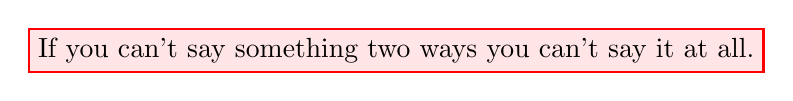
\begin{tikzpicture}
        \node[draw=red, fill=red!10, thick]
            {If you can't say something two ways you can't say it at all.};
    \end{tikzpicture}
\end{center}

This credo may seem odd to linguists, who usually take a strongly realist stance according to which the grammar formalism fully specifies the grammar, even down to notation.
For example, privative (= single-valued) and binary features are regarded as vastly different objects that make very different claims about phonology.
Yet we will see at a later point that they are but two definitions of the same computational object.
That does not rule out that one of the two is a more useful way of thinking about phonology, but that is a matter of epistemology rather than ontology.

\begin{definition}[Bigrams]
    Given a string $w$ over alphabet $\Sigma$, its \emph{augmented} counterpart $\augmented{w} \is \LeftEdge \stringcat w \stringcat \RightEdge$ is obtained by adding the left and right edge markers $\LeftEdge$ and $\RightEdge$ to $w$, where $\LeftEdge$ and $\RightEdge$ are distinguished symbols not contained in $\Sigma$.
    Furthermore, 
    \(
    \Bigrams(w) \is
        \setof{
            \ngram{ab} \mid \exists u,v \in \Sigma^* \text{ s.t.\ }
                u \stringcat \ngram{ab} \stringcat v = \augmented{w}
        }
    \)
    denotes the set of \emph{bigrams} over $\augmented{w}$, i.e.\ the smallest set that contains all substrings of $\augmented{w}$ that consist of exactly $2$ symbols.
\end{definition}

\begin{definition}[Bigram Grammar]
    A \emph{bigram grammar} $G$ over alphabet $\Sigma$ is a finite set of bigrams over $\Sigma \cup \setof{\LeftEdge, \RightEdge}$.
    If $G$ is a \emph{positive bigram grammar} (denoted $\posG{G}$), then it generates the language
    \(
        L(G) \is \setof{
            w \mid \Bigrams(w) \subseteq G
        }
    \).
    If $G$ is a \emph{negative bigram grammar} (denoted $\negG{G}$), then it generates the language
    \(
        L(G) \is \setof{
            w \mid \Bigrams(w) \cap G = \emptyset
        }
    \).
\end{definition}

With all these definitions under our belt, we can finally move on to producing a new insight: positive and negative bigram grammars are equally powerful.
That is to say, if some language is generated by a positive bigram grammar, then it can also be generated by some negative bigram grammar, and the other way round.

\begin{theorem}
    The class of languages that are generated by positive bigram grammars is exactly the class of languages that are generated by negative bigram grammars.
    \label{thm:SL_PosNegEquivalence}
\end{theorem}
%
In order to show that this theorem is indeed correct, we establish two simpler propositions --- called lemmata --- which jointly imply the theorem.

\begin{lemma}
    For every positive bigram grammar there is a negative bigram grammar that generates the same language.
    \label{lem:SL_Pos2Neg}
\end{lemma}
%
\begin{proof}
    Let $\posG{G}$ be a positive bigram grammar. 
    We show that $\negG{\complementof{G}}$ defines the same language as $\posG{G}$, where $\complementof{G}$ consists of all bigrams over $\Sigma \cup \setof{\LeftEdge, \RightEdge}$ that are not contained by $G$.

    Pick some arbitrary string $w \in L(\posG{G})$. 
    By definition, every bigram of $w$ is a member of $G$, which immediately implies that no element of $\Bigrams(w)$ is contained in $\complementof{G}$.
    But if none of the bigrams of $w$ belong to $\complementof{G}$, then $\Bigrams(w) \cap \complementof{G} = \emptyset$, wherefore $w \in L(\negG{\complementof{G}})$.
    Since $w$ was arbitrary, this result holds for every string generated by $\posG{G}$, establishing $L(\posG{G}) \subseteq L(\negG{\complementof{G}})$.

    The same argument can be applied in the other direction to show $L(\posG{G}) \supseteq L(\negG{\complementof{G}})$, wherefore $L(\posG{G}) = L(\negG{\complementof{G}})$.
\end{proof}
%
This is a so-called \emph{constructive} proof: we do not just show that an equivalent negative bigram grammar exists, we also explain how this grammar can be constructed from the positive bigram grammar.
Constructive proofs are the most useful kind of proof because they provide procedures and strategies that can be implemented and run automatically.

In the case at hand, all we have to do in order to construct an equivalent negative bigram grammar is to take the set-theoretic complement of the positive bigram grammar.
After all, the set of all bigrams over $\Sigma$ is given by $\Sigma \times \Sigma$, and the positive bigram grammar $\posG(G)$ is some subset thereof (\emph{modulo} edge markers, which are treated as part of $\Sigma$ here to avoid notational clutter).
Bigrams that belong to $G$ may occur in a string, bigrams that do not must not.
So the bigrams not belonging to $G$ are the illicit bigrams, which means those are exactly the bigrams the equivalent negative bigram grammar must contain.
In one sentence: taking the complement of $G$ is like taking its negation, and the switch from a positive grammar to a negative one undoes this negation.

So now we know that the negative bigram grammars are at least as powerful as the positive bigram grammars since the latter can be translated into the former.
It only remains for us to show that the same holds in the other direction.

\begin{lemma}
    For every negative bigram grammar there is a positive bigram grammar that generates the same language.
\end{lemma}
%
\begin{proof}
    Left as an exercise to the reader.
\end{proof}

\subsection{The How and Why of Proofs}

Proofs are a difficult art at every level of expertise.
For the beginner, the biggest challenge is often to sort out their train of thought and present it in a clear manner: where do I start, and how do I proceed from there step by step to reach the conclusion?

There are no clear-cut rules here, but it is often helpful to break up the problem into smaller ones, as we did with Thm.~\ref{thm:SL_PosNegEquivalence}.
If two sets $A$ and $B$ need to be shown to be equivalent, one can first prove $A \subseteq B$ and then $B \subseteq A$.
And a statement of the form ``$\phi$ iff $\psi$'' can be broken up into ``$\phi$ entails $\psi$'' and ``$\psi$ entails $\phi$''.
We will encounter several basic proof techniques throughout the course (proof by induction, indirect proofs), but don't worry too much about specific techniques for now.
Instead, make sure to work through the proofs we discuss multiple times until you understand how they work.
Always try to answer the following questions for yourself:

\begin{itemize}
    \item Why is the initial assumption valid?
    \item How does each conclusion follow from the previous one?
    \item Why does the final conclusion show that the theorem\slash lemma is correct?
\end{itemize}

You may wonder why we need proofs in the first place.
Linguists don't work with proofs yet they have discovered a lot of interesting things about language.
Programmers don't have much use for proofs either.
There's several answers, the simplest one being that some questions can only be addressed conclusively via proofs.
Consider the following alternative to the proof of Lem.~\ref{lem:SL_Pos2Neg}: we could have implemented the translation procedure from positive to negative grammars and then tested it on a large sample of positive bigram grammars (at least several thousand).
Eventually the program would have told us that the negative grammars generate the same string languages as their positive counterparts.
So if the conversion works correctly on every single one of thousands of positive bigram grammars, isn't that enough to posit that positive and negative bigram grammars are interchangeable?

The answer is No.
First of all, checking that two grammars generate the same language is hardly trivial if both languages are infinite (we can't just compare all their respective members).
More importantly, though, the thousands of test grammars may accidentally share a special property that is essential for the correctness of the conversion.
This is a real risk if all those test grammars were automatically generated by a script because true randomness is very hard to achieve with computers, if not impossible.
While experiments and simulations have their place --- they are a valid last resort where proofs are hard to come by --- a proof is always the preferred solution where possible.

Proofs are preferred not only because they are safe from the pitfalls of simulations, but also because they provide genuine insight.
In fact, proofs are often more important and enlightening than the theorems they establish.
Testing the correctness of the bigram conversion via automated experiments could at best show us whether the procedure is correct (if there's only finitely many cases to test), but it does not tell us \textbf{why}.
A proof is an explicit record of how certain properties entail others.
In the case at hand, it is the close connection between set-theoretic complementation and the switch from positive to negative grammars that does all the work.
Notice all the properties of bigram grammars that the proof does not depend on: that bigrams are strings, that bigrams consist of exactly two symbols, and that bigram grammars are finite. 
Yet these properties necessarily hold during any test procedure, so we would not be able to tell which one of them is a prerequisite for the correctness of the conversion.
Thanks to the proof, we know which properties matter, which in turn might come in handy in the study of other formalisms.

In a few lines, a proof can establish unassailable truths, show us why they hold, but also save us hours of work compared to running simulations.
So even though you may initially find them hard and time consuming, proofs are actually the tool of choice for the lazy scientist.


\section{Linguistic Evaluation}
The bigram grammar model improves on the list phonology model in various respects.
Variation across languages is now much more restricted because phonology is just a collection of highly local constraints (negative bigram grammars) or permissions (positive bigram grammars).
Bigram grammars also account for linguistic creativity, i.e.\ that speakers can form new words according to the rules of their own language, and that they recognize whether nonce words are well-formed.
As a consequence, they do not predict that the lexicon is finite, either.
Whether the lexicon is finite or infinite is immaterial for bigram grammars since they determine well-formedness in a compositional manner.
As long as each word is finite, its grammaticality can easily be determined via a bigram scanner.

Bigram grammars do still exhibit isolationism and egalitarianism.
Since a grammar is a list of bigrams, all these bigrams should have the same status and there should be no distictions between easy and difficult processes.
And processes still cannot apply across words: for \emph{phone bill}, the phonological representation is presumably something like \LeftEdge\textipa{foUn}\RightEdge\LeftEdge\textipa{bIl}\RightEdge.
Since \textipa{n} and \textipa{b} are not adjacent, a negative bigram grammar with \ngram{nb} does not have the desired result.
This could be fixed with a bigger search domain, though, which also seems to be necessary for slightly less local processes like intervocalic voicing, where we want to block a voiceless sound only if it occurs between two vowels.

Overall bigram grammars are doing very well on a conceptual level and are easy to implement, but they are not expressive enough for English.
Next time we will see how we can keep all their attractive properties while increasing their power to a more adequate level.

%hw: does this model have smaller memory usage? By how much?

\chapter{Extending Bigram Grammars}
\label{cha:SLMath}

Bigram grammars are a step in the right direction from the initial list phonology model.
Every grammar is still just a list of items, but now we use this list to determine the well-formedness of a word in a compositional manner.
The problem of bigram grammars is that they are not powerful enough to capture certain phonological processes like intervocalic voicing --- in linguistic parlance, the size of the grammars' locality domain is limited to two adjacent symbols, so bigger contexts cannot be represented correctly.
The obvious solution is to extend the size of the scanner window so that the grammar uses trigrams, 4-grams, or maybe even something bigger.
We will see today that this generalization is a natural one in the sense that it preserves the essential properties of bigram grammars while increasing their empirical coverage.

\section{Generalization to Strictly Local Grammars}

Lifting the notion of bigrams to arbitrary $k$-grams works almost exactly as one would suspect.
The set of trigrams of the string $\String{abcd}$, for example, includes $\String{\LeftEdge a b}$, $\String{abc}$, $\String{bcd}$, and $\String{cd\RightEdge}$.
However, it also includes $\String{\LeftEdge \LeftEdge a}$ and $\String{d \RightEdge \RightEdge}$.
Why the extra trigrams with multiple edge markers?
For one thing, we still want to directly express basic facts like ``a word may start with $a$'', while the trigram $\String{\LeftEdge a b}$ encodes ``a word may start with $a$ followed by $b$''.
More importantly, as the length of $k$-grams increase, more and more words won't have a single $k$-gram unless we pad them with $k-1$ edge markers.
For example, the augmented version of the empty string would just be $\LeftEdge \RightEdge$, which is too short for a trigram.
Similarly, the string $\String{ab}$ would be $\String{\LeftEdge ab \RightEdge}$, which is too short any $k$-gram with $k > 4$.
The simplest solution is to simply add $k-1$ edge markers instead of just a single one.
For bigrams, the number of edge markers does not change since $2 - 1 = 1$.

On the formal side, the generalization from bigrams to $k$-grams requires but a few minor modifications in our original definition.
We also use this opportunity to slightly change our terminology: instead of \emph{$k$-gram grammar} and \emph{$k$-gram languages}, we will speak of \emph{strictly $k$-local grammars} and \emph{strictly $k$-local languages}.
This will make it easier later on to distinguish this formalism from a related one that also operates with $k$-grams but interprets them differently.

\begin{definition}[$k$-grams]
    Let $k$ be some natural number.
    A \emph{$k$-gram}, or \emph{$k$-factor}, over alphabet $\Sigma$ is an element of $(\Sigma \cup \setof{\LeftEdge, \RightEdge})^k$.
    Given a string $w$ over $\Sigma$, its \emph{$k$-augmented} counterpart $\augmented{w}_k \is \LeftEdge^{k-1} \stringcat w \stringcat \RightEdge^{k-1}$ consists of $w$ with $k-1$ left edge markers and $k-1$ right edge markers, and its set of $k$-grams is given by
    \(
        \Bigrams[k](w) \is
            \setof{
                s \in (\Sigma \cup \setof{\LeftEdge, \RightEdge})^k
                \mid
                \exists u,v \in \Sigma^* \text{ s.t. }
                u \stringcat s \stringcat v = \augmented{w}
            }
    \).
\end{definition}
%
You can see that this definition of $k$-gram is a natural extension of the concept of bigrams for if we replace $k$ by $2$ in the definition, we get exactly the original definition of bigrams.
The concept of bigram languages is generalized in the same fashion to $k$-gram languages, which jointly form the class of \emph{strictly local languages}.
%
\Note{%
    Notice that the definition of strictly $k$-local also allows for $k = 0$.
    Can you list all strictly $0$-local languages?
    \emph{Hint}: There's only two of them.
}
%
\begin{definition}[Strictly Local Languages]
    A finite set of $k$-grams is called a \emph{strictly $k$-local grammar}.
    A positive strictly $k$-local grammar $G$ generates the language
    \(
        L(G) \is
            \setof{ w \mid \Bigrams[k](w) \subseteq G }
    \).
    A negative strictly $k$-local grammar $G$ generates the language
    \(
        L(G) \is
            \setof{ w \mid \Bigrams[k](w) \cap G = \emptyset }
    \).
    A language $L$ is \emph{strictly $k$-local} iff it is generated by some strictly $k$-local grammar.
    The class of \emph{strictly local languages} is given by
    \(
        \bigcup_{k \geq 1} \setof{ L \mid L \text{ is strictly $k$-local} }
    \).
\end{definition}
%
Intuitively, a language is strictly local iff all its well-formedness conditions are restricted to a locality domain of finitely bounded size.
\Note{At first glance it seems that the grammars in Fig.~\ref{fig:SL_Scanner} and~\ref{fig:SLMath_Scanner} generate the same language, but that is not the case.
What is the difference between the respective languages?}
This also means that every strictly local language can be recognized by a scanner that can adapt the size of its search window to any finite size depending on the grammar the scanner operates with.
Figure~\ref{fig:SLMath_Scanner} shows such a scanner working with a positive strictly $4$-local grammar.
%
\begin{figure}[tbph]
\centering
\begin{tikzpicture}
    \begin{scope}[spy using outlines={rectangle, size = 5em}]
        % input string    
        \foreach \Name/\Symbol in { 0/$\LeftEdgeSymbol$,
                                    1/$\LeftEdgeSymbol$,
                                    2/$\LeftEdgeSymbol$,
                                    3/$a$,
                                    4/$b$,
                                    5/$a$,
                                    6/$b$,
                                    7/$a$,
                                    8/$b$,
                                    9/$a$,
                                    10/$b$,
                                    11/$a$,
                                    12/$b$,
                                    13/$b$,
                                    14/$\RightEdgeSymbol$,
                                    15/$\RightEdgeSymbol$,
                                    16/$\RightEdgeSymbol$
                                  }
            \node[text height=.75em] (\Name) at ($(\Name*1.5em,0)$) {\Symbol};

        % arrow for scanner direction
        \draw[blue,->] (5.north) to (9.north);

        % list of bigrams
        \node (bigrams) at (7.south)
            [
            yshift=-18em,
            minimum width=7em,
            minimum height=7.5em,
            fill=red!5,
            draw=red,
            thick,
            rounded corners
            ]
            {%
                \begin{tabular}{l}
                    \\[-.5em]
                    $\LeftEdge \LeftEdge \LeftEdge a$\\
                    $\LeftEdge \LeftEdge a b$\\
                    $\LeftEdge a b a$\\
                    $a b a b$\\
                    $b a b a$\\
                    $b a b \RightEdge$\\
                    $a b \RightEdge \RightEdge$\\
                    $b \RightEdge \RightEdge \RightEdge$\\
                \end{tabular}%
            };

        % name of list of bigrams
        \node (G) at (bigrams.north)
            [
            minimum width=7em,
            fill=red,
            draw=red,
            thick,
            rounded corners
            ]
            {\color{white}\textbf{Grammar}};

        % frame for looking up first scanned bigram 
        \draw[thick,gray,fill=gray!50,opacity=.3] ($(bigrams.west)+(1em,3.35em)$) rectangle ($(bigrams.east)+(-1em,2.35em)$);

        % frame for failed looked up of second scanned bigram
        \node[xshift=3em,yshift=-2em, thick,draw=gray,fill=gray!50,opacity=.3,align=center] (failed) at (bigrams.east) {\phantom{error}};
        \node at (failed) {error};

        % first scanner window
        %---------------------
        % create center coordinate for zoom target
        \coordinate (zoomcenter-good) at ($(1.east) !.5! (4.west)$);

        % spy on zoom target, create node (zoom) below
        \spy[magnification=2,
             blue,
             width = 11em,
             spy connection path={
                \draw[dashed] (tikzspyonnode.north west) -- (tikzspyinnode.north west);
                \draw[dashed] (tikzspyonnode.north east) -- (tikzspyinnode.north east);
                \draw[dashed] (tikzspyonnode.south west) -- (tikzspyinnode.south west);
                \draw[dashed] (tikzspyonnode.south east) -- (tikzspyinnode.south east);
                \draw[dashed,gray] (tikzspyinnode.south) ..
                                            controls +(245:8em) and +(170:3em) ..
                                                ($(bigrams.west)+(1em,2.85em)$);
            }]
            on (zoomcenter-good) in node [fill=blue!5] (zoom-good) at ($(zoomcenter-good) - (0,8em)$);


        % second scanner window
        %----------------------
        % create center coordinate for zoom target
        \coordinate (zoomcenter-bad) at ($(10.east) !.5! (13.west)$);

        % spy on zoom target, create node (zoom) below
        \spy[magnification=2,
             blue,
             width = 11em,
             spy connection path={
                \draw[dashed] (tikzspyonnode.north west) -- (tikzspyinnode.north west);
                \draw[dashed] (tikzspyonnode.north east) -- (tikzspyinnode.north east);
                \draw[dashed] (tikzspyonnode.south west) -- (tikzspyinnode.south west);
                \draw[dashed] (tikzspyonnode.south east) -- (tikzspyinnode.south east);
                \draw[dashed,gray] (tikzspyinnode.south) ..
                                            controls +(300:6em) and +(30:6em) ..
                                                (failed.east);
            }]
            on (zoomcenter-bad) in node [fill=blue!5] (zoom-bad) at ($(zoomcenter-bad) - (0,8em)$);

    \end{scope}
\end{tikzpicture}

\caption{Scanner for a positive strictly $4$-local grammar}
\label{fig:SLMath_Scanner}
\end{figure}
%
\begin{examplebox}[A Strictly $3$-Local Grammar for $(\String{aba})^+$]
    Consider the language $(\String{aba})^+$, which consists of the strings $\String{aba}$, $\String{abaaba}$, $\String{abaabaaba}$, and so on.
    This language is not strictly $2$-local, because any positive strictly $2$-local grammar that generates the string $\String{abaaba}$ must contain the bigram $\String{aa}$ and thus would also generate any string of the form $\String{abaa^+ba}$.
    But there is a positive strictly $3$-local grammar that generates the language:
    %
    \begin{center}
        \begin{tabular}{lll}
            $\LeftEdge \LeftEdge a$
            &
            \String{aba}
            &
            \String{ba \RightEdge}
            \\
            \String{\LeftEdge a b }
            &
            \String{baa}
            &
            $a \RightEdge \RightEdge$
            \\
            &
            \String{aab}
        \end{tabular}
    \end{center}
    %
    Substituting C for $a$ and V for $b$, we can conclude from this example that natural languages with a CVC syllable template require a locality domain of at least $3$.
\end{examplebox}
\Note{The example only shows that no \emph{positive} strictly $2$-local grammar generates $\String{(aba)^+}$, but this implies that no negative strictly $2$-local grammar can generate it either.
If this is not immediately apparent to you, reread chapter~\ref{cha:SL}.}

The phonological processes we have looked at so far --- word-final devoicing, nasal assimilation, and intervocalic devoicing --- are all strictly local.
The first two are strictly 2-local, the third one strictly 3-local.
%
\begin{examplebox}[Intervocalic Voicing is Strictly 3-Local]
    It is easy to see that intervocalic voicing cannot be captured with strictly $2$-local grammars.
    Suppose the language under investigation contains the words \textipa{bIsta} and \textipa{bItsa}.
    Any positive strictly $2$-local grammar generating these two strings contains at least the bigrams \LeftEdge\textipa{b}, \textipa{bI}, \textipa{Is}, \textipa{sa}, and \textipa{a\RightEdge}.
    Consequently, whatever language it generates must contain the string \textipa{bIsa}, which violates intervocalic voicing.

    A negative strictly $3$-local grammar, on the other hand, can easily enforce intervocalic voicing.
    It only needs to contain all trigrams of the form $\String{UsV}$, where $U$ and $V$ are vowels and $s$ is some voiceless consonant.
\end{examplebox}
%
It is also readily apparent that constraints on syllable structure are strictly local.
Take some language that only allows for syllables of the form V, VC, CV, and CVC, but not CCV, VCC, CVCC, or CCVCC\@.
In other words, a well-formed word cannot contain more than two consecutive consonants, and these consonants cannot occur at the beginning or the end of the word, where they would necessarily be part of the same syllable.
The set of illicit substrings, then, consists of \LeftEdge CC, CCC, and CC \RightEdge.
This can be compiled out into a set of illicit sequences of phones by substituting for each C the phones that are specified for [+cons].
So this example of a restricted syllable template does note exceed the power of a negative strictly $3$-local grammar.

If desired, the negative strictly local grammar can be converted into a positive one using our standard procedure.
\Note{Why does equivalence of positive and negative grammars break down for strictly $0$-local grammars?}
Go back to the proof of our theorem that positive and negative bigram grammars are equivalent, and you will see that it does not rely on the length of the $k$-grams being $2$.
Therefore the theorem can be trivially generalized to all strictly $k$-local grammars ($k \geq 1$).

We could spend much more time designing strictly local grammars for other local processes in phonology, e.g.\ assimilation across word boundaries, vowel harmony, umlaut, or spirantization.
As long as these processes describe surface true generalizations --- that is to say, they do not make reference to an underlying form and can be stated purely in terms of which output forms are licit --- writing down the grammars might require quite a bit of ink, but very little genuine thought.
Notice that these processes must be local but can nonetheless be globally unbounded.
Vowel harmony, for instance, may apply throughout an entire word via a sequence of local vowel harmony steps.
%
\begin{examplebox}[Strictly $4$-Local Vowel Harmony]
    Suppose language $L$ has an alphabet with two vowels, $i$ and $u$, and two consonants $p$ and $l$.
    All words match the syllable template (CVC)$^+$.
    In addition, $i$ triggers progressive vowel harmony that turns each $u$ following an $i$ into $i$.
    Consequently, no surface form may contain an $i$ followed by a $u$.
    Assuming that no other processes or constraints apply in $L$, the language is strictly $4$-local.

    We first construct a positive strictly $4$-local grammar $\posG{S}$ for the syllable template.
    This grammar contains all $4$-grams, and only those, that can be obtained from the entries below by substituting $i$ and $u$ for occurrences of V and $p$ and $l$ for occurrences of C (which yield a total of 76 $4$-grams).
    %
    \begin{center}
        \begin{tabular}{lll}
            \LeftEdge\LeftEdge\LeftEdge C
            &
            C V C C
            &
            C V C \RightEdge
            \\
            \LeftEdge\LeftEdge C V
            &
            V C C V
            &
            V C \RightEdge\RightEdge
            \\
            \LeftEdge C V C
            &
            C C V C
            &
            C \RightEdge\RightEdge\RightEdge
        \end{tabular}
    \end{center}
    %
    Vowel harmony is enforced by the negative strictly $4$-local grammar $\negG{V}$ with the $4$-grams $\String{ilpu}$ and $\String{iplu}$.
    We then convert $\posG{S}$ into an equivalent negative grammar and take their union.
    A brief moment of reflection reveals that $L(\negG{\complementof{S}} \cup \negG{V}) = L$.
\end{examplebox}
%
\Note{Give a rough approximation of the size of $\negG{\complementof{S}}$ and compare it to $\negG{V}$.
    Does the size difference match your intuition about the complexity of the respective phonotactic constraints encoded by these grammars?
}
%
Locally bounded processes giving rise to locally unbounded dependencies is exactly what we expect given how strictly local grammars operate: the $k$-grams only regulate the shape of local domains, but the well-formedness of the word is evaluated by moving through the word and checking each local domain.
So not only are strictly local grammars powerful enough to capture local well-formedness conditions in phonology, the way they enforce them mirrors linguists' intuitions about how local processes can produce global patterns.

The connection between strictly local grammars and local processes in phonology allows us to study the latter through the former.
Since strictly local grammars generate strictly local languages, this implies that the properties of strictly local languages can tell us something about local processes in phonology.
Let us repeat this for emphasis:
%
\begin{center}
    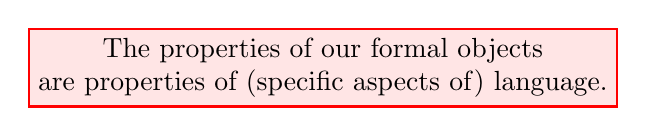
\begin{tikzpicture}
        \node[draw=red, fill=red!10, thick, align=center]
            {The properties of our formal objects\\ are properties of (specific aspects of) language.};
    \end{tikzpicture}
\end{center}
%
The theoretical task of proving formal properties of strictly local languages has suddenly morphed into an empirically minded investigation of phonology.

\section{Exploring Strictly Local Languages}

\subsection{A Proper Hierarchy of Strictly Local Languages}
The examples discussed so far suggest that the power of strictly local grammars increases with the size of the locality domain.
This is indeed the case, but is best proved by recourse to the strictly local languages.
If we order the strictly local languages by the size of their locality domain, we get a proper hierarchy: one level properly subsumes the next.
Denoting the class of strictly $k$-local languages by $\SL_k$, we have $\SL_k \subsetneq \SL_{k-1}$ for all $k \geq 0$.

This is a complex claim, as it asserts that each strictly $k$-local language is strictly $k+1$-local, but that the opposite does not hold for some languages.
Following our standard strategy, we establish lemmata for these weaker claims and then combine them into the original theorem.
%
\begin{lemma}
    It holds for every $k \geq 0$ that if language $L$ is strictly $k$-local, then $L$ is also $k+1$-local.
\end{lemma}
%
The proof for this lemma is slightly more complicated than anything we have seen so far, but behind the notation lies a very simple idea:
the size of the locality domain can be increased from $k$ to $k+1$ by padding the edge markers and by combining two overlapping $k$-grams into a single $k+1$-gram.
Consequently, for every strictly $k$-local grammar there is an equivalent strictly $k+1$-local one.
%
\begin{proof}
    If $L$ is strictly $k$-local then it is generated by some positive strictly $k$-local grammar $G$ over some alphabet $\Sigma$.
    Let $G'$ be the smallest set such that for all $k$-grams $g_1, g_2 \in G$
    %
    \begin{itemize*}
        \item if $g_1$ starts with $\LeftEdge$, then $\LeftEdge g_1 \in G'$,
        \item if $g_1$ ends with $\RightEdge$, then $g_1 \RightEdge \in G'$,
        \item if $g_1 \is a_1 a_2 \cdots a_{k}$ and $g_2 \is a_2 \cdots a_k a_{k+1}$, then $a_1 a_2 \cdots a_k a_{k+1} \in G'$.
    \end{itemize*}
    %
    Clearly $G'$ is finite and can therefore be interpreted as a positive $k+1$-local grammar.
    We show that $L = L(G')$, thus establishing that $L$ is $k+1$-local.
    
    If $w \in L(G')$, then $\Bigrams[k+1](w)$ is a subset of $G'$.
    All $k+1$-grams with multiple edge markers have a corresponding $k$-gram with one edge marker less, which is contained in $G$.
    All other $k+1$-grams are split into two $k$-grams by removing the first or the last symbol.
    Each $k$-gram is once again contained in $G$, so $\Bigrams[k](w) \subseteq G$ and hence $w \in L(G) = L$.
    Since $w$ was arbitrary we have $L(G') \subseteq L$.

    If $w \in L$, then $\Bigrams[k](w)$ is a subset of $G$.
    Assume towards a contradiction that $\Bigrams[k+1](w)$ is not a subset of $G'$.
    Then $w$ contains some $k+1$-gram $g_3$ that is not a member of $G$.
    If $g_3$ starts or ends with two edge markers, then the corresponding $k$-gram with only one of the two markers cannot have been part of $G$, contradicting our initial assumption.
    In all other cases, $g_3$ is built from two overlapping $k$-grams $g_1$ and $g_2$, at least one of which is not contained in $G$.
    But then $\Bigrams[k](w)$ is not a subset of $G$, contradicting once more our initial assumption.
    It follows, then, that $\Bigrams[k+1](w)$ is a subset of $G'$ after all, wherefore $L \subseteq L(G')$.
\end{proof}
%
\begin{examplebox}[Converting Bigrams Into Trigrams]
    Consider the strictly $2$-local language $(\String{ab})^+$ and its positive strictly $2$-local grammar $G$ with the bigrams $\LeftEdge a$, $\String{ab}$, $\String{ba}$, and $b\RightEdge$.
    In order to construct an equivalent strictly $3$-local grammar, we have to pad out the edge markers and combine overlapping bigrams.
    So $\LeftEdge a$ and $b \RightEdge$ become $\LeftEdge\LeftEdge a$ and $\RightEdge\RightEdge b$, respectively.
    We also see that $\LeftEdge a$ overlaps with $\String{ab}$, so we can combine them into $\String{\LeftEdge a b}$.
    The same procedure produces $\String{ab \RightEdge}$ from $\String{ab}$ and $b \RightEdge$.
    Finally, $\String{ab}$ and $\String{ba}$ overlap in two ways depending on which one is put in front of the other, so that we obtain two trigrams from them: $\String{aba}$ and $\String{bab}$.
    This exhausts the number of possible combinations. 
    The strictly $3$-local grammar is shown below:
    %
    \begin{center}
        \begin{tabular}{lll}
            \String{\LeftEdge\LeftEdge a}
            &
            \String{aba}
            &
            \String{b \RightEdge\RightEdge}
            \\
            \String{\LeftEdge a b}
            &
            \String{bab}
            &
            \String{a b \RightEdge} 
        \end{tabular}
    \end{center}
    %
    This grammar generates all strings of $(\String{ab})^+$, and only those.
\end{examplebox}

\begin{lemma}
    For every $k$ there is some strictly $k+1$-local language that is not strictly $k$-local.
    \label{lem:SLMath_SL-HierarchyProper}
\end{lemma}
%
\begin{proof}
\Note{%
    This proof uses a finite language, but the lemma holds even if we only consider infinite languages.
    Try to generalize the proof along these lines.
}
    Consider the finite language $L$ that contains only the string $a^k$, i.e.\ the string with $k$ consecutive $a$s.
    It is generated by the strictly $k+1$-local grammar $\setof{\LeftEdge a^k, a^k \RightEdge}$.
    However, $\Bigrams[k](a^k) = \setof{\LeftEdge a^{k-1}, a^k, a^{k-1} \RightEdge} = \Bigrams[k](a^n)$ for every $n \geq k$, so a strictly $k$-local grammar that generates $a^k$ also generates all these $a^n$ and thus a proper superset of $L$.
\end{proof}
%
\begin{theorem}
    For all $k \geq 0$, $\SL_k \subsetneq \SL_{k+1}$.    
\end{theorem}

Now we know for sure that the size of the locality domain has a direct effect on generative capacity.
This is hardly surprising, but still far from trivial --- in Chapter~\ref{cha:REG} we will encounter a very similar formalism for which all $k \geq 2$ have exactly the same power.


\subsection{Relation to Finite Languages}

Remember that the list phonology model of Lecture~\ref{cha:ListPhonology} was restricted to lists of finite length, so it could only generate finite languages.
This restriction is empirically inadequate as it conflicts with the assumption that the list of phonological words in a given natural language is infinite and fails to handle nonce words and linguistic creativity in general.
But not only is the list phonology model restricted to finite languages, it adds insult to injury with its ability to generate all finite languages.
Every finite language is a viable natural language phonology according to the list model, and we have already seen why this is typologically untenable.
The class of finite languages is the class that is least likely to provide an insightful or empirically adequate model of language, so we should strive to work with formalisms that cannot generate this class.

The strictly local languages are a marked improvement over the list phonology model in this respect, but only if one adopts the right perspective.
First, it is obvious that strictly local languages can be infinite, so not every strictly local language is finite.
Let us make this claim fully explicit via a proof.
We already know that every strictly $k$-local language is strictly $k+1$-local, so all we need is an example of a language that is both infinite and strictly $1$-local language.

\Note{%
Further reflection reveals that almost every $1$-local language is infinite.
In fact, there are only two $1$-local languages that are finite.
Can you define them?
\emph{Hint}: One of them is strictly $0$-local.
}
%
\begin{lemma}
    There is a strictly $1$-local language that is infinite.
\end{lemma}
%
\begin{proof}
    Let $\posG{G} \is \setof{\LeftEdge, a, \RightEdge}$.
    Then $L(\posG{G}) = \setof{\emptystring, a, \String{aa}, \String{aaa}, \ldots} = a^*$, which is infinite.
\end{proof}
%
\begin{corollary}
    For every $k \geq 1$, $\SL_k$ contains an infinite language.
\end{corollary}
%
This is a welcome result because it shows that no matter what size of locality domain we pick, we are never restricted to just finite languages.
An even more appealing property of strictly local languages is that for every level of the infinite hierarchy there are some finite languages that cannot be defined.
Consequently, strictly local grammars improve on the list phonology model in that they cannot define just about any arbitrary phonological systems.
%
\begin{theorem}
    For every $k \geq 1$, there is some finite language that is not contained in $\SL_k$. 
\end{theorem}
%
\begin{proof}
    Pick an infinite language that is generated by some strictly $k$-local grammar $G$ over alphabet $\Sigma$.
    Discard from $G$ all $k$-grams that start with $\LeftEdge$ or end in $\RightEdge$.
    The resulting set is a finite language $L$.
    We show that $L$ is not strictly $k$-local.

    Since $G$ generates an infinite set, it must contain (not necessarily distinct) $k$-grams $a \stringcat u$ and $u \stringcat b$, where $a,b \in \Sigma$ and $u \in \Sigma^{k-1}$.
    Note that both $a \stringcat u$ and $u \stringcat b$ belong to $L$, whereas $a \stringcat u \stringcat b$ does not.
    But $\Bigrams[k](a \stringcat u) \cup \Bigrams[k](u \stringcat b) = \Bigrams[k](a \stringcat u \stringcat b)$, and consequently every strictly $k$-local grammar that generates $a \stringcat u$ and $u \stringcat b$ also generates $a \stringcat u \stringcat b$.
    Hence $L$ is not strictly $k$-local.
\end{proof}
%
The proof above is rather sneaky.
It exploits the fact that every strictly $k$-local grammar is a finite set of strings of length $k$, but this very set can also be viewed as a finite language.
This is an interesting perspective: a strictly $k$-local grammar $G$ is a finite language $L_G$ coupled with a specific algorithm $A$ for creating a new language from $L_G$.
If we try to generate $L_G$ via a second strictly $k$-local grammar, this grammar automatically uses the algorithm $A$, so for certain choices of $L_G$ the grammar generates additional strings via $A$ that do not belong to $L_G$.

Viewing grammars as languages will seem odd to many linguists, who think of the grammar as the knowledge the speaker has acquired about their language, whereas the language is the output produced from this knowledge.
But that is an ontological distinction.
It is a useful distinction to make when outlining the research program of linguistics, its goals, problems, and promises.
It highlights that modern linguistics is about human cognition rather than merely describing individual languages as abstract systems of structures and rules that exist independent of the speaker's cognitive ability to use them.
The latter view dates back to Structuralism, and there are good reasons why it was abandoned.
As useful as the ontological mandate may be, though, it has no say over what mathematical tricks we may avail ourselves of.
Equating grammars with languages can be useful in some cases.
Here it furnishes a proof about the limits of strictly local languages, and in Ch.~\ref{cha:Derivations} it will open up completely new methods of constructing syntactic grammars.

If you still find all of this horribly confusing, do not despair:
there is a much simpler proof that does not blur the distinction between grammars and languages and instead uses the same trick that we already encountered in the proof of Lem.~\ref{lem:SLMath_SL-HierarchyProper}.
%
\begin{proof}
    Consider the finite language that consists only of the string $a^k$.
    Note that $\Bigrams[k](a^k) = \setof{\LeftEdge a^{k-1}, a^k, a^{k-1} \RightEdge} = \Bigrams[k](a^{k+1})$.
    Thus every strictly $k$-local grammar that generates $a^k$ also generates $a^{k+1}$.
    This entails that no strictly $k$-local grammar generates the finite language $\setof{a^k}$.
\end{proof}
%
Why would anyone ever want to use the more complicated proof if there is a much simpler one?
In poetic terms: because the journey is the destination.
Proofs aren't just about establishing results, they tell us why a specific result holds and hence provide us with deeper insights.
The simpler proof does not highlight that each strictly local grammar it itself a finite language, an obvious yet nonetheless surprising fact.
New perspective like this are always useful.
Remember the Keenan-Moss credo:
%
\begin{center}
    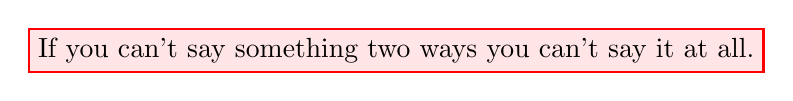
\begin{tikzpicture}
        \node[draw=red, fill=red!10, thick]
            {If you can't say something two ways you can't say it at all.};
    \end{tikzpicture}
\end{center}
%
This isn't restricted to definitions, it also extends to proofs.
The more routes take us towards a specific result, the better.

One important point that both proofs share is that they presuppose that the size of the locality domain is fixed to some $k$.
Hence they do not apply if we consider the whole class of strictly local languages, which turns out to properly subsume the class of finite languages.
%
\begin{theorem}
    Every finite language is strictly local.
\end{theorem}
%
\begin{proof}
    Suppose that $L$ is a finite language, the longest string of which has length $k - 1$, $k \geq 1$.
    We define a $k$-local grammar $G$ that consists of the $k$-grams $\LeftEdge^i \stringcat w \stringcat \RightEdge^j$, where $w \in L$, $w$ has length $l < k$, and $i + j + l = k$.
    Since every $k$-gram starts with $\LeftEdge$ or ends in $\RightEdge$, $L(G) = L$, wherefore $L$ is strictly $k$-local.
\end{proof}
%
We see that the relation between strictly local languages and finite languages is more involved than one would expect.
Without restrictions on the size of the locality domain, the strictly local languages include all finite languages.
However, the class of strictly $k$-local languages and the class of finite languages are incomparable --- they have a non-empty intersection, but neither subsumes the other (cf.\ Fig.~\ref{fig:SLMath_SL-Fin}).
So assuming that $k$ is fixed for natural language phonology, e.g.\ as part of Universal Grammar, strictly local grammars are a good approximation of local processes in phonology.
They can handle infinity and do not incorrectly predict languages to vary freely across all dimensions.
In particular, they naturally give rise to iterated local processes such as progressive vowel harmony.
%
\begin{figure}[htpb]
    \centering
    \begin{tikzpicture}[
    lang/.style = {rounded corners, thick, fill, fill opacity=.5}
    ]
    \node (sl0) at (0,0) {$\SL_0$};
    \node (sl1) at (4em,0) {$\SL_1$};
    \node (sln) at (10em,0) {$\SL_n$};
    \node (sl) at (16em,0) {$\SL$};
    
    \node (fin) at (-6em,0) {$\FIN$};

    \node (dots1) at ($(sl1) !.5! (sln)$) {\ $\cdots$};
    \node (dots1) at ($(sln) !.5! (sl)$) {\ $\cdots$};

    % rectangles for language classes
    \begin{pgfonlayer}{background}
        % SL 
        \draw[lang,blue!45] ($(fin.north west)+(-1.5em,2.5em)$) rectangle ($(sl.south east)+(1.5em,-2.5em)$);

        % SL_n
        \draw[lang,blue!15] ($(sl0.north west)+(-2em,1.25em)$) rectangle ($(sln.south east)+(.5em,-1.25em)$);

        % SL_1
        \draw[lang,blue!10] ($(sl0.north west)+(-1em,.5em)$) rectangle ($(sl1.south east)+(.5em,-.5em)$);
        
        % SL_0
        \draw[lang,blue!5] ($(sl0.north west)+(-.5em,.25em)$) rectangle ($(sl0.south east)+(.5em,-.25em)$);

        % Fin
        \draw[lang,red!35] ($(fin.north west)+(-1em,2em)$) rectangle ($(fin.south east)+(4em,-2em)$);
    \end{pgfonlayer}
\end{tikzpicture}

    \caption{Relation between strictly local and finite languages}
    \label{fig:SLMath_SL-Fin}
\end{figure}

\subsection{Substring Substitution Closure}
\label{sub:SLMath_SubstitutionClosure}

In several of the preceding proofs we have used the fact that a strictly local grammar sometimes ``overshoots the target''.
A finite language $L$ may not be in $\SL_k$ because a strictly $k$-local grammar that tries to generate $L$ will also end up generating other strings outside of $L$.
But a strictly $k+1$-local grammar may be able to do a point landing and generate all and only those strings that are members of $L$.
What this shows is that a strictly $k$-local grammar only has perfect precision within its locality domain of size $k$, beyond that it has to generalize.
This generalization step is what allows strictly local grammars to generate infinite languages, making it the true source of their power.

Crucially, though, strictly local grammars don't just generalize randomly, quite to the contrary: all strictly local grammars generalize in the same fashion, irrespective of the size of their locality domain.
Their generalization strategy is already implicit in the definition of strictly local languages, which categorizes strings as well-formed or ill-formed according to their set of $k$-grams.
If two strings have exactly the same set of $k$-grams, then either both are well-formed or both are ill-formed.

But it is quite hard to tell what this condition implies for the overall shape of the string languages.
Given a string language $L$, how can we tell whether $L$ is strictly local?
Fortunately strictly local languages are uniquely characterized by a property called \emph{substring substitution closure}.
%
\begin{definition}[Local Substring Substitution Closure]
    A language $L$ satisfies \emph{$k$-local substring substitution closure} iff there is some $k \geq 1$ such that if $L$ contains both $u \stringcat x \stringcat v$ and $u' \stringcat x \stringcat v'$, where $x$ has length $k - 1$, then $L$ also contains $u \stringcat x \stringcat v'$.
\end{definition}
%
\begin{theorem}
    A language is in $\SL_k$ iff it satisfies $k$-substring substitution closure.
\end{theorem}
%
Let us look at a couple of examples first before wading through the proof of the theorem.

\begin{examplebox}[A Substring Substitution Closed Language]
    We have already seen that the language $(\String{ab})^+$ is strictly $2$-local as it is generated by the grammar $\setof{\LeftEdge a, \ngram{ab}, \ngram{ba}, b \RightEdge}$.
    Now we can also verify this via substring substitution closure.
    For instance, we can line up $\String{abab}$ and $\String{abababab}$ to show that the language must also contain $\String{ababab}$.
    %
    \[
        \begin{array}{rcll}
                          & x &              & \\
            \String{ab}   & a & \String{b}   & \in L\\
            \String{abab} & a & \String{bab} & \in L\\\hline
            \String{ab}   & a & \String{bab} & \in L
        \end{array}
    \]
    %
    Notice how $x$ is a single symbol since its length must be $k-1 = 2 - 1 = 1$.
    Also, we could have established the membership of $\String{ababab}$ more succinctly using just $\String{abab}$ or $\String{abababab}$.
    \[
        \begin{array}{rcll}
                        & x &              & \\
            \String{ab} & a & \String{b}   & \in L\\
                        & a & \String{bab} & \in L\\\hline
            \String{ab} & a & \String{bab} & \in L
        \end{array}
        %
        \qquad
        %
        \begin{array}{rcll}
                          & x &                & \\
            \String{ab}   & a & \String{babab} & \in L\\
            \String{abab} & a & \String{bab}   & \in L\\\hline
            \String{ab}   & a & \String{bab}   & \in L
        \end{array}
    \]
\end{examplebox}
%
Since substring substitution closure fails if even a single string is missing from the set, it is usually not a good way of showing that a language is strictly local --- if the language in question is infinite, one cannot show via specific substitutions that it is suffix substitution closed.
However, suffix substitution closure is an excellent way of showing that a language is \textbf{not} strictly local by giving a single example of a missing string.
%
\begin{examplebox}[A Language that Fails Subtree Substitution Closure]
    Consider the language $(\String{aa})^+$, the variant of $(\String{ab})^+$ where all $b$s have been replaced by $a$s.
    This language is not strictly local as it fails $k$-local substring substitution closure for any choice of $k$.
    Suppose $k$ is an even number:
    %
    \[
        \begin{array}{rcll}
            & x & & \\
        a & a \cdots a & a & \in L \\
          & a \cdots a &   & \in L \\\hline
        a & a \cdots a &   & \notin L\\
        \end{array}
    \]
    %
    A minimally different pattern is used if $k$ is odd.
    No matter what the value of $k$, the language is not suffix substitution closed and thus not strictly local.
    You might find this surprising given that the only difference to $(\String{ab})^+$ is the replacement of $b$ by $a$.
    This highlights another property of strictly local languages: the alphabet plays a crucial role in what languages are definable.
\end{examplebox}
%
\begin{proof}
    We now show that a language $L$ is strictly $k$-local iff it is closed under $k$-local substring substitution.
    
    \paragraph{Left to right}
    Note first that substring substitution closure is trivially satisfied if $L$ contains no strings of length strictly greater than $k-1$, for then all strings take the form $\emptystring \stringcat x \stringcat \emptystring$ with respect to $k$-local substring substitution.
    Suppose, then, that $s_1$ and $s_2$ are strings of $L$ with length strictly greater than $k-1$ such that $s \is u_1 \stringcat x \stringcat v_1$ and $s_2 \is u_2 \stringcat x \stringcat v_2$.
    If $s_1 = s_2$, then $u_1 \stringcat x \stringcat v_2 = s_1 = s_2$, so substring substitution closure is not violated.
    If $s_1 \neq s_2$, then it must be the case that $\Bigrams[k](u_1 \stringcat x \stringcat v_2) \subseteq \Bigrams[k](s_1) \cup \Bigrams[k](s_2) \subseteq G$, where $G$ is a strictly $k$-local grammar with $L(G) = L$.
    It follows immediately that $s_1 \stringcat x \stringcat v_2$ is a member of $L(G)$ and thus a member of $L$. 
    This exhausts all possible cases, showing that $L$ is indeed closed under $k$-local substring substitution.

    \paragraph{Right to left}
    Suppose $L$ is closed under $k$-local substring substitution, and let $G \is \bigcup_{w \in L} \Bigrams[k](w)$ be a positive strictly $k$-local grammar.
    It suffices to establish $L(G) = L$, which entails that $L$ is strictly $k$-local.

    It is easy to see from the definition of $G$ that $L \subseteq L(G)$.
    Showing that $L(G) \subseteq L$ requires a fairly lengthy proof that is omitted here.
    The curious reader is referred to \citet[19--21]{Rogers07}.
\end{proof}

\subsection{Closure Properties}

Suffix substitution closure is --- as its name implies --- a \emph{closure property}.
One says that an object $o$ is closed under an operation iff applying this operation to elements of $o$ yields only elements of $o$.
In other words, the operation never takes us outside of $o$.
The natural numbers, for instance, are closed under addition since the sum of two natural numbers is yet again a natural numbers.
But they are not closed under subtraction because, say, $2-5$ yields $-3$, which is an integer but not a natural number.
Suffix substitution closure simply means that a language is closed under the operation of substituting suffixes in a specific way.

But of course there are many other operations that can be applied to a language, and it will be interesting to see whether strictly local languages are closed under them.
In particular the basic set-theoretic operations of intersection, union, and relative complement are of interest since they tell us how we can build strictly local languages from smaller ones.

Let us look at closure under intersection first.
This one is particularly important because of the close correspondence that negative strictly local grammars establish between constraints on the one hand and languages on the other.
If every $k$-gram corresponds to a well-formedness constraints, then one would expect that one can get the intersection of two languages by simply conjoining their respective well-formedness constraints.
That is indeed the case.
%
\begin{lemma}
    The class of strictly $k$-local languages is closed under intersection, $k \geq 0$.
\end{lemma}
%
\begin{proof}
    We prove that for any two strictly local languages generated by (positive) grammars $G_1$ and $G_2$, $L(G_1) \cap L(G_2) = L(G_1 \cap G_2)$.
\Note{Give an analogous proof using negative grammars.}
    We first show $L(G_1) \cap L(G_2) \subseteq L(G_1 \cap G_2)$.
    Let $w$ be an arbitrary string belonging to both $L(G_1)$ and $L(G_2)$, i.e.\ $w \in L(G_1) \cap L(G_2)$.
    Then every $k$-gram of $w$ is contained in both $G_1$ and $G_2$, so $w \in L(G_1 \cap G_2)$.
    Since $w$ is arbitrary, we have $L(G_1) \cap L(G_2) \subseteq L(G_1 \cap G_2)$.
    The same reasoning can be applied in the other direction, yielding $L(G_1 \cap G_2) \subseteq L(G_1) \cap L(G_2)$.
    These two facts jointly imply $L(G_1) \cap L(G_2) = L(G_1 \cap G_2)$.
\end{proof}
%
% fixme: hw: spell out the second subset relation
%
Closure under intersection, too, can be used to prove that a language is not strictly local.
Suppose we know that $L$ is strictly local, but we have a hard time showing that $L'$ is not strictly local.
Then we can instead try to show that $L \cap L'$ is not strictly local, as this immediately implies the non-locality of $L'$, too.
%
% fixme: example!

One might expect that closure under union holds too since one can simply take the union of the grammars, but this does not work as expected.
The union of two grammars $G_1$ and $G_2$ often generates a superset of the union of $L(G_1)$ and $L(G_2)$.
Do not even try to look for a smarter strategy to build a grammar for the union of two strictly local languages, there is none that works in all cases.
%
\begin{lemma}
    The class of strictly local languages is not closed under union. 
\end{lemma}
%
\begin{proof}
    We give an example of two bigram languages whose union is not a bigram language.
    The proof can easily be adapted for arbitrary values of $k$.

    Let $L_1 \is \setof{\mathit{ab}}$ and $L_2 \is \setof{\mathit{b}, \mathit{bb}, \mathit{bbb}, \ldots}$.
    \Note{``w.l.o.g.''\ is short for ``without loss of generality'' and is meant to indicate that the proof can easily be adapted to cases that are not covered by the assumption.}
    Assume w.l.o.g.\ that all bigram grammars are positive.
    Then any bigram grammar that generates $L_1$ must contain the bigrams $\LeftEdge a$, $\mathit{ab}$, and $b \RightEdge$.
    Similarly, a bigram grammar generating $L_2$ must contain the bigrams $\LeftEdge b$, $\mathit{bb}$, and $b \RightEdge$.
    Therefore a bigram grammar that generates all strings in $L_1 \cup L_2$ must contain at least these bigrams.
    But such a grammar also generates the string $\mathit{abb}$, which is not part of $L_1 \cup L_2$.
    Hence there is no bigram grammar that generates all the strings in $L_1 \cup L_2$ and nothing else, so $L_1 \cup L_2$ is not a bigram language.
\end{proof}
%
Abstract as it may be, this result is of immediate importance for our investigation of phonology.
If the union of two arbitrary strictly local languages were also strictly local, then we would expect that phonological processes can always apply disjunctively.
Consider the following example: some languages have sibilant harmony, while others have vowel harmony.
Each process can be equated with the set of strings that satisfy the respective harmony pattern.
If we take the union of these two sets, we get the set of strings that satisfy sibilant harmony or vowel harmony.
If that set were intersected with some natural language's phonology --- which is an abstract way of saying that we force the constraint represented by that set onto the language --- then words in that language are well-formed as long as they obey sibiliant harmony or vowel harmony, but they need not obey both.
This is extremely unnatural. If a language has two phonological processes, then words must usually obey both.
It is not the case that satisfying one constraint grants you \emph{carte blanche} to ignore the other.
The closure properties of strictly local languages can explain this fact: intersection (= constraint conjunction) always yields a potential natural language phonology, union (=constraint disjunction) may not.
The assumption that local phonological processes fit within the bounds of strictly local languages thus makes a typological prediction: if two constraints apply in a disjunctive fashion as indicated above, then these two constraints must be such that their union is also strictly local --- which rules out a great number of strictly local languages.
%
%fixme: hw: extend proof to case where both languages are infinite
%fixme: hw: extend proof to arbitrary k

The previous two lemmata also imply that closure under relative complement does not hold.
%
\begin{lemma}
    The class of strictly local languages is not closed under (relative) complement.
\end{lemma}
%
\begin{proof}
    By De Morgan's law $L_1 \cup L_2 = \complementof{\complementof{L_1} \cap \complementof{L_2}}$.
    If the class of strictly local languages were closed under both complement and intersection, it would thus be closed under union, too.
    Since closure under intersection holds while closure under union does not, closure under relative complement cannot hold, either.
\end{proof}
%
%fixme: hw: give a proof by example
You may find this result surprising because the complement of a strictly local grammar is a strictly local grammar.
But in general $\complementof{L(G)}$ differs from $L(\complementof{G})$, just like $L(G_1) \cup L(G_2)$ is not guaranteed to be $L(G_1 \cup G_2)$.
These differences illustrate why it is so important to distinguish between grammars and the languages they generate.

We finish with yet another missing closure property.
%
\begin{lemma}
    The class of strictly local languages is not closed under relabelings.
\end{lemma}
%
% fixme: define relabeling
%
\begin{proof}
    We have already seen that $(ab)^+$ is strictly 2-local whereas the relabeling $(aa)^+$ is not strictly local at all.
    But the former is the image of the latter under a relabeling that replaces all $b$s by $a$s.
\end{proof}
%
This is a very important result as it ties directly into the abstractness debate in generative phonology.
Suppose that we are allowed to have all kinds of hidden structure in our phonological representation, e.g.\ a basic syllable template or feet.
Then we could assume that the language $(aa)^+$ is underlyingly equipped with a CV-template, so that we should rather think of it as $(a_C a_V)^+$.
This language is strictly local (it is a notational variant of $(ab)^+$), so $(aa)^+$ is strictly local under a mapping that removes unpronounced structure.
In Chapter~\ref{cha:REG} we will see that this is a very dangerous route to take: hidden structure pushes strictly local languages to a level of power where all phonological processes are equally simple.
This eradicates all distinctions between processes and takes us back to the undesirable egalitarianism of the list phonology model.

\section{Implications for Phonology}
Our mathematical expedition has taught us a surprising amount about phonology.
First of all, all local phonological dependencies (including those spanning across word boundaries) can be handled by strictly local grammars, a very simple formalism with few cognitive requirements.
The model comes with a minimal memory burden as it only requires the speaker to keep track of a small number of $k$-factors.
It is also very fast: recognition via a scanner takes linear time and can be carried out in an incremental online fashion.
Lookup of $k$-factors in the grammar takes at most logarithmic time using binary search, and even faster search methods can be implemented.
With a hash table, lookup is instantaneous.

But strictly local grammars also capture essential properties of phonological competence.
They are analytic in nature and thus capable of generating infinite languages, which solves the problems the list phonology model had with linguistic creativity and nonce words.
The special relation between strictly $k$-local languages and finite languages also means that certain typological pitfalls are avoided.
Not every random collection of strings is predicted to be a valid phonological system, and grammars generating an infinite language generalize in a linguistically plausible fashion by determining the well-formedness of strings as a composite function of the local domains.

We have also seen that strictly local languages lack closure properties that do not hold of natural languages either.
The union or relative complement of a natural language's phonotactics is not guaranteed to be a valid phonological system for a natural language, just like the class of strictly local languages is not closed under these operations.
The increase of power brought about by relabelings also cautions us against using hidden structures and highly abstracted alphabets, an issue that has been discussed at length in phonology and that will occupy us at various points for the rest of the course.

%fixme: non-closure under composition
%       contrast with closure properties of FIN

%fixme:
%hw: complete proof of positive-negative equivalence
%hw: implement k to k+1 converter

\chapter{Strict Locality: Alternative Characterizations}
\label{cha:SLImplement}

The previous chapter was all about extending bigram grammars to strictly local grammars while changing as little about our perspective as possible.
This chapter does the exact opposite.
Following the Keenan-Moss credo of saying something in as many ways as possible, we take a look at several distinct characterizations of strict locality.
We start out simple by exploring different methods to represent and store strictly local grammars.
This reinforces the message of Ch.~\ref{cha:Formal} about Marr's levels of description: the further we move away from the computational level towards the algorithmic level, the more implementation details do we have to take care of that may have an effect on runtime behavior and overall performance but are ultimately immaterial for the computational properties we are interested in.
The second half of the chapter then moves on to characterizations of strict locality that are less directly tied to grammars: automata and a specific fragment of propositional logic. 

\section{Implementations of Strictly Local Grammars}

\subsection{Prefix Trees Revisited}

The discussion of the list phonology model in Ch.~\ref{cha:ListPhonology} spent quite some time on how such a list can be efficiently searched and stored.
Prefix trees turned out to be ideal for this purpose as they provide a more compact representation but can also be searched very quickly --- finding an item only requires following one specific branch for each sound in the word.
It doesn't take much ingenuity to realize that strictly local grammars, too, can be stored as prefix trees.
%
\begin{examplebox}[Prefix Tree for a Strictly 4-Local Grammar]
    Consider the strictly $4$-local grammar, which was also used in Fig~.\ref{fig:SLMath_Scanner}.
    \label{ex:SLImplement_PrefixTree}
    %
    \begin{center}
        \begin{tabular}{lll}
            $\LeftEdge \LeftEdge \LeftEdge a$
            &
            $a b a b$
            &
            $b a b \RightEdge$
            \\
            $\LeftEdge \LeftEdge a b$
            &
            $b a b a$
            &
            $a b \RightEdge \RightEdge$
            \\
            $\LeftEdge a b a$
            &
            &
            $b \RightEdge \RightEdge \RightEdge$
        \end{tabular}
    \end{center}
    %
    This set corresponds to the prefix tree below, where nodes are numbered for the sake of exposition.
    
    \begin{tikzpicture}[
        state/.style = {circle, fill=blue!15, inner sep = 0pt, minimum width = 2em},
        final/.style = {circle, fill=red!15, inner sep = 0pt, minimum width= 2em},
        keylabel/.style = {black},
        arc/.style = {->,gray!75}
        ]
        \node[state] (root) {0};
            \node[state] (L) [below left=of root] {1};
                \node[state] (LL) [below left=of  L] {2};
                    \node[state] (LLL) [below left=of LL] {3};
                        \node[final] (LLLa) [below=of LLL] {4};
                    \node[state] (LLa) [below=of LL] {5};
                        \node[final] (LLab) [below=of LLa] {6};
                \node[state] (La) [below=of L] {7};
                    \node[state] (Lab) [below=of La] {8};
                        \node[final] (Laba) [below=of Lab] {9};
            \node[state] (a) [below=of root] {10};
                \node[state] (ab) [below=of a] {11};
                    \node[state] (aba) [below=of ab] {12};
                        \node[final] (abab) [below=of aba] {13};
                    \node[state] (abR) [below right=of ab] {14};
                        \node[final] (abRR) [below=of abR] {15};
            \node[state] (b) [below right=of root] {16};
                \node[state] (ba) [below=of b] {17};
                    \node[state] (bab) [below right=of ba] {18};
                        \node[final] (baba) [below=of bab] {19};
                        \node[final] (babR) [below right=of bab] {20};
                \node[state] (bR) [below right=of b] {21};
                    \node[state] (bRR) [below right=of bR] {22};
                        \node[final] (bRRR) [below right=of bRR] {23};

        \foreach \Source/\Target/\Label in {%
            root/L/$\LeftEdge$,
            L/LL/$\LeftEdge$,
            LL/LLL/$\LeftEdge$,
            LLL/LLLa/a,
            LL/LLa/a,
            LLa/LLab/b,
            L/La/a,
            La/Lab/b,
            Lab/Laba/a,
            root/a/a,
            a/ab/b,
            ab/aba/a,
            aba/abab/b%
            }
            \draw[arc] (\Source) to node [left,keylabel] {\Label} (\Target);

        \foreach \Source/\Target/\Label in {%
            ab/abR/$\RightEdge$,
            abR/abRR/$\RightEdge$,
            root/b/b,
            b/ba/a,
            ba/bab/b,
            bab/baba/a,
            bab/babR/$\RightEdge$,
            b/bR/$\RightEdge$,
            bR/bRR/$\RightEdge$,
            bRR/bRRR/$\RightEdge$%
            }
            \draw[arc] (\Source) to node [right,keylabel] {\Label} (\Target);
    \end{tikzpicture}
    
    The prefix tree has lots of unary branches that can be compressed further to yield a radix tree.

    \begin{tikzpicture}[
        state/.style = {circle, fill=blue!15, inner sep = 0pt, minimum width = 2em},
        final/.style = {circle, fill=red!15, inner sep = 0pt, minimum width= 2em},
        keylabel/.style = {black},
        arc/.style = {->,gray!75}
        ]
        \node[state] (root) {0};
            \node[state] (L) [below left=4.5em of root] {1};
                \node[state] (LL) [below left=of  L] {2};
                    \node[final] (LLLa) [below left=of LL] {4};
                    \node[final] (LLab) [below=of LL] {6};
                \node[final] (Laba) [below=of L] {9};
                \node[state] (ab) [below=of root] {11};
                    \node[final] (abab) [below left=2em of ab] {13};
                    \node[final] (abRR) [below right=2em of ab] {15};
            \node[state] (b) [below right=4.5em of root] {16};
                \node[state] (bab) [below=of b] {18};
                        \node[final] (baba) [below=of bab] {19};
                        \node[final] (babR) [below right=of bab] {20};
                \node[final] (bRRR) [below right=of b] {23};

        \foreach \Source/\Target/\Label in {%
            root/L/$\LeftEdge$,
            L/LL/$\LeftEdge$,
            LL/LLLa/$\LeftEdge$a,
            LL/LLab/ab,
            L/Laba/aba,
            root/ab/ab,
            ab/abab/ab%
            }
            \draw[arc] (\Source) to node [left,keylabel] {\Label} (\Target);

        \foreach \Source/\Target/\Label in {%
            ab/abRR/$\RightEdge\RightEdge$,
            root/b/b,
            b/bab/ab,
            bab/baba/a,
            bab/babR/$\RightEdge$,
            b/bRRR/$\RightEdge\RightEdge\RightEdge$%
            }
            \draw[arc] (\Source) to node [right,keylabel] {\Label} (\Target);
    \end{tikzpicture}
\end{examplebox}

As you seen from the example above, the prefix\slash radix trees for strictly local grammars differ slightly from those for the list phonology model in that they have only leaf nodes as final states.
% fixme: was final state mentioned before?
So we do not need to encode the distinction between final and non-final states, saving us a tiny amount of memory (1 bit per node in the tree).

You might have also noticed that some branches are duplicated.
To give but one example, the nodes 11 and 21 in the prefix tree of example~\ref{ex:SLImplement_PrefixTree} share the same sub-branch \RightEdge-\RightEdge.
We can combine these branches by first merging the nodes 14 and 22, and then 15 and 23.
This does not change the grammar because the set of paths from a root to a leaf has not changed --- in particular, we have not lost the paths a-b-\RightEdge-\RightEdge and b-\RightEdge-\RightEdge-\RightEdge, and we have not gained any new paths.
If we had merged 14 and 23 instead just because they both are reached via a \RightEdge arc, then we would have lost the path a-b-\RightEdge-\RightEdge and gained the path a-b-\RightEdge.
This would have changed the grammar to an extent where it wouldn't even be strictly 4-local anymore according to our definition.
Nor is it licit to merge 7 and 17 because they both can be continued by the sub-path b-a.
If we did that, we would lose no paths, but suddenly \LeftEdge-a-b-\RightEdge would be a possible path and the grammar would be able to generate $\String{ab}$.
So it is important to verify that nodes are merged only if that does not affect the set of paths from the root to a leaf.
%
\begin{examplebox}[DAG for Strictly $4$-Local Grammar]
    The prefix tree from example~\ref{ex:SLImplement_PrefixTree} can be converted into the graph shown below.
    \label{ex:SLImplement_DAG}
    Note that nodes are no longer color-coded to distinguish final from non-final states since all leaf nodes are final, and only those.
    %
    \begin{center}
        \begin{tikzpicture}[
    state/.style = {circle, fill=blue!15, inner sep = 0pt, minimum width = 2em},
    final/.style = {circle, fill=red!15, inner sep = 0pt, minimum width= 2em},
    keylabel/.style = {black},
    arc/.style = {->,gray!75}
    ]
    \node[state] (root) {0};
        \node[state] (L) [below left=of root] {1};
            \node[state] (LL) [below=of  L] {2};
                \node[state] (LLL) [below left=of LL] {3};
                    \node[state] (LLLa) [below=of LLL] {\footnotesize 4,9,19};
                \node[state] (LLa) [below=of LL] {\footnotesize 5,12};
                    \node[state] (LLab) [below=of LLa] {\footnotesize 6,13};
            \node[state] (La) [below left=of L] {7};
                \node[state] (Lab) [below left=of La] {8};
        \node[state] (a) [below=of root] {10};
            \node[state] (ab) [below=of a] {11};
        \node[state] (b) [below right=of root] {16};
            \node[state] (ba) [below right=of b] {17};
                \node[state] (bab) [below right=of ba] {18};
            \node[state] (bR) [below=of b] {21};
                \node[state] (bRR) [below right=of bR] {\footnotesize 14,22};
                    \node[state] (bRRR) [below right=of bRR,align=center] {\footnotesize 15,20,\\\footnotesize23};

    \foreach \Source/\Target/\Label in {%
        root/L/$\LeftEdge$,
        L/LL/$\LeftEdge$,
        LL/LLL/$\LeftEdge$,
        LLL/LLLa/a,
        LL/LLa/a,
        LLa/LLab/b,
        L/La/a,
        La/Lab/b,
        Lab/LLLa/a,
        root/a/a,
        a/ab/b,
        ab/LLa/a%
        }
        \draw[arc] (\Source) to node [left,keylabel] {\Label} (\Target);

    \foreach \Source/\Target/\Label in {%
        ab/bRR/$\RightEdge$,
        root/b/b,
        b/ba/a,
        ba/bab/b,
        bab/bRRR/$\RightEdge$,
        b/bR/$\RightEdge$,
        bR/bRR/$\RightEdge$,
        bRR/bRRR/$\RightEdge$%
        }
        \draw[arc] (\Source) to node [right,keylabel] {\Label} (\Target);

    \draw[arc,bend left=8] (bab) to node [below,keylabel] {a} (LLLa);
\end{tikzpicture}

    \end{center}
    %
    This graph can be compacted even further by removing unary branching nodes in the same fashion that converts a prefix tree into a radix tree.
    %
    \begin{center}
        \begin{tikzpicture}[
    state/.style = {circle, fill=blue!15, inner sep = 0pt, minimum width = 2em},
    final/.style = {circle, fill=red!15, inner sep = 0pt, minimum width= 2em},
    keylabel/.style = {black},
    arc/.style = {->,gray!75}
    ]
    \node[state] (root) {0};
        \node[state] (L) [below left=of root] {1};
            \node[state] (LL) [below=of  L] {2};
                \node[state] (LLLa) [below left=of LL,yshift=-4em] {\footnotesize 4,9,19};
                \node[state] (LLa) [below=of LL] {\footnotesize 5,12};
                    \node[state] (LLab) [below=of LLa] {\footnotesize 6,13};
            \node[state] (Lab) [below left=8em of L] {8};
        \node[state] (ab) [below=8em of root] {11};
        \node[state] (b) [below right=of root] {16};
            \node[state] (bab) [below right=10em of b] {18};
            \node[state] (bRR) [below=7.5em of b] {\footnotesize 14,22};
                \node[state] (bRRR) [below right=of bRR,align=center] {\footnotesize 15,20,\\\footnotesize23};

    \foreach \Source/\Target/\Label in {%
        root/L/$\LeftEdge$,
        L/LL/$\LeftEdge$,
        LL/LLLa/$\LeftEdge$a,
        LL/LLa/a,
        LLa/LLab/b,
        L/Lab/ab,
        Lab/LLLa/a,
        root/ab/ab,
        ab/LLa/a%
        }
        \draw[arc] (\Source) to node [left,keylabel] {\Label} (\Target);

    \foreach \Source/\Target/\Label in {%
        ab/bRR/$\RightEdge$,
        root/b/b,
        b/bab/ab,
        bab/bRRR/$\RightEdge$,
        b/bRR/$\RightEdge\RightEdge$,
        bRR/bRRR/$\RightEdge$%
        }
        \draw[arc] (\Source) to node [right,keylabel] {\Label} (\Target);

    \draw[arc,bend left=8] (bab) to node [below,keylabel] {a} (LLLa);
\end{tikzpicture}

    \end{center}
    %
    Note that the graph differs from the one one would obtain from the radix tree in example~\ref{ex:SLImplement_PrefixTree} by merging nodes.
    In particular, the former has 12 nodes and the latter 13.
\end{examplebox}

Once we start merging trees, prefix trees are no longer trees because some nodes have more than one mother.
Linguists call such trees \emph{multi-dominance trees}.
This term ins unknown in computer science, and instead one speaks of \emph{directed acyclic graphs} (DAGs).
DAGs are slightly more general than multi-dominance trees because they can have multiple roots.
%
\begin{definition}[DAG]
    A \emph{graph} is a pair $\tuple{V,E}$ consisting of a set $V$ of \emph{vertices} and a set $E \subseteq V \times V $ of \emph{edges} connecting vertices.
    We also speak of \emph{nodes} and \emph{branches}, respectively.
    The reflexive, transitive closure of $E$ is denoted $E^*$.
    A \emph{directed acyclic graph} is a graph that satisfies the following axiom:
    %
    \begin{description}
        \item[No cycles] for all $u,v \in V$, $\tuple{u,v} \in E$ implies $\tuple{v,u} \notin E^*$.
    \end{description}
    %
    A graph\slash DAG is \emph{edge-labeled} iff it comes equipped with a function $\LabelFunc: E \rightarrow \Omega$ that assigns each edge $e \in E$ some symbol drawn from the alphabet $\Omega$ of edge labels.
\end{definition}
%
\begin{techinfo}[Closure of a Relation]
    In Cha.~\ref{cha:SLMath} we encountered the notion of \emph{closure} in the sense that a given object may be closed under some operation.
    A slightly different sense of \emph{closure} is commonly used to construct new relations from old ones.
    Suppose $R$ is some relation over set $S$, i.e.\ $R \subseteq S \times S$.
    Then for $P$ some property of relations, the $P$-closure of $R$ is the smallest relation $R'$ such that $R \subseteq R' \subseteq S \times S$ and $R'$ satisfies property $P$.
    Here are three common properties that are used in this connection:
    %
    \begin{description}
        \item[reflexive] $\tuple{u,u} \in R$ (for all $u \in S$)
        \item[symmetric] $\tuple{u,v} \in R$ implies $\tuple{v,u} \in R$ (for all $u,v \in S$)
        \item[transitive] $\tuple{u,v} \in R$ and $\tuple{v,w} \in R$ jointly imply $\tuple{u,w} \in R$ (for all $u,v,w \in S$)
    \end{description}
    %
    The linguistic notion of proper dominance in a tree, for example, is the transitive closure of the mother-of relation.
    Reflexive dominance, on the other hand, is the reflexive transitive closure of the mother-of relation.
\end{techinfo}

\subsection{Matrices}

While tree-based representations are very convenient for humans, it is far from obvious how one could implement them in some programming language.
There exist specialized libraries for Python (search for \emph{py-dag} and \emph{marisa-trie}), but in general it is prudent to keep the number of dependencies for a program as small as possible without sacrificing essential functionality.
In many cases, a simpler solution is to switch to a different representation format that is easier to use.
For graphs there already is a well-known strategy: reencode them as \emph{adjacency matrices}.
An adjacency matrix has a row and a column for each node, and the value in row $i$ and column $j$ is $x$ iff the graph contains an edge that spans from $i$ to $j$ and is labeled $x$.
%
\begin{examplebox}[Adjacency Matrix for a Radix Tree]
    The radix-like DAG from example~\ref{ex:SLImplement_DAG} corresponds to the adjacency matrix below.
    \label{ex:SLImplement_AdjacencyMatrix}
    %
    {
    \small
        \[
        \begin{blockarray}{rcccccccccccc}
            & 0 & 1 & 2 & 4,9,19 & 5,12 & 6,13 & 8 & 11 & 14,22 & 15,20,23 & 16 & 18\\ 
            \begin{block}{r(cccccccccccc)}
                0 & & \LeftEdge & & & & & & \String{ab} & & & \String{b}\\
                1 & & & \LeftEdge & & & & \String{ab}\\
                2 & & & & \String{\LeftEdge a} & \String{a}\\
                4,9,19 & \\
                5,12 & & & & & & \String{b}\\
                6,13 & \\
                8 & & & & \String{a}\\
                11 & & & & & \String{a} & & & & \String{\RightEdge}\\
                14,22 & & & & & & & & & & \String{\RightEdge}\\
                15,20,23 & \\
                16 & & & & & & & & & & & & \String{ab}\\
                18 & & & & & & & & & & \String{\RightEdge}\\
            \end{block}
        \end{blockarray}
        \]
    }
\end{examplebox}
%
While Python does not include matrices as a basic data type (in contrast to \emph{R}), a 2-dimensional matrix can be treated as a list of lists.
Listing~\ref{code:SLImplement_Graph2Matrix} gives a Python function for converting graphs into this format and gives an example of how such lists can be queried.
%
\begin{listing}[tbph]
\pythonfile[firstline=5]{./code/matrices/graph2matrix.py}

\medskip
\begin{pythoncode}
    >>> graph = {
    ...     ['A', 'B', 'C'],
    ...     [
    ...         ('A', 'B', 'e'),
    ...         ('A', 'C', 'f'),
    ...         ('B', 'B', 'g'),
    ...         ('C', 'A', 'h'),
    ...         ('C', 'C', 'i')
    ...     ]
    ... ]
    >>> graph2matrix(graph)
    [['', 'e', 'f'], ['', 'g', ''], ['h', '', 'i']]
    >>> graph2matrix(graph)[graph[0].index('A')][graph[0].index('B')]
    'e'
\end{pythoncode}
\caption{Python function for converting graphs to adjacency matrices}
\label{code:SLImplement_Graph2Matrix}
\end{listing}

While definitely useful, adjacency matrices make it very hard for humans to determine at a glance what grammar they encode.
It is far from obvious that the table in example~\ref{ex:SLImplement_AdjacencyMatrix} encodes the same information as the set of $4$-grams we started out with at the beginning of the chapter.
That's not surprising, as the matrix is the output of a long chain of information-preserving transformations: from a set of $4$-grams to a prefix tree to a DAG to a compacted DAG to an adjacency matrix.
%
\Note{%
    \begin{center}
        \includegraphics[width=.8\linewidth]{./img/pic/boole}

        \noindent
        \textbf{George Boole}
    \end{center}

    The term Boolean was coined in honor of \emph{George Boole}, one of the founding fathers of mathematical logic whose work is the theoretical foundation of the switching circuits used in computer hardware.
    Like many great thinkers, he died prematurely.
    Unlike most great thinkers, he has his wife to blame for that.
}
%
A slightly more intuitive route directly translates a strictly $k$-local grammar into a $k$-dimensional \emph{Boolean matrix}.
A Boolean matrix requires each cell to have the value True\slash 1 or False\slash 0.
The idea is that we can map each symbol of our alphabet to a unique natural number such that if the Boolean matrix has a 1 in cell $i_1, \ldots, i_k$, then the grammar contains a $k$-gram $s_1 \cdots s_k$ iff $i_j$ is the natural number assigned to symbol $s_j$ for all $1 \leq j \leq k$.
That is quite a mouthful, but hopefully a quick example will make things clearer.
%
\begin{examplebox}[Strictly $k$-Local Grammar as $k$-Dimensional Matrix]
    Suppose that our alphabet contains only the symbols $a$ and $b$, plus the two edge markers.
    We randomly assign all four symbols natural numbers.
    The assignment below will work just fine for our purposes:
    %
    \begin{center}
        \begin{tabular}{ccc}
            $\LeftEdge$  & $\mapsto$ & 0\\
            $a$          & $\mapsto$ & 1\\
            $b$          & $\mapsto$ & 2\\
            $\RightEdge$ & $\mapsto$ & 4
        \end{tabular}
    \end{center}
    %
    Now consider the familiar strictly $2$-local grammar $\setof{\String{\LeftEdge a}, \String{ab}, \String{ba}, \String{b \RightEdge}}$ for the string language $(\String{ab})^+$.
    We can represent this grammar as a $2$-dimensional Boolean matrix.
    %
    \[
        \begin{pmatrix}
            0 & 1 & 0 & 0\\
            0 & 0 & 1 & 0\\
            0 & 1 & 0 & 1\\
            0 & 0 & 0 & 0\\
        \end{pmatrix}
    \]
    %
    Here rows represent the first symbol of the bigrams, columns the second symbol.
    The first column is completely filled by 0s because no bigram in the grammar contains $\LeftEdge$ in the second position.
    The second column represents the possibility of $a$ occurring in second position.
    As it has the form $(1,0,1,0)$, $a$ may occur in second position only if the first position is filled by $\LeftEdge$ or $b$.
    The remaining two columns encode the possible combinations for $b$ and $\RightEdge$ in second position.

    Alternatively, we could have gone through the matrix row by row rather than column by column.
    In that case, the $i$-th row tells us whether the symbol mapped to index $i$ can occur in first position depending on the second symbol.
\end{examplebox}
%
Boolean matrices have several technical advantages which we will not discuss here.
Quite simply, they constitute a very restricted and well-understood type of matrix, and consequently there are many efficient algorithms for working with them.
For our purposes, this is yet another way of looking at strictly local grammars, but one that will gel exceptionally well with certain (probabilistic) extensions presented in Ch.~\ref{cha:PSL}.

\section{Automata}

Our initial discussion of strictly $2$-local grammars in Ch.~\ref{cha:SL} was quick to point out that a grammar by itself only defines the set of well-formed structures --- determining whether a specific input belongs to that set requires a recognizer.
We picked scanners as the recognizers for strictly local grammars.
But that does not mean that scanners are the only conceivable type of recognizer for these grammars.
If one combines our previous discussion of graphs with our knowledge of scanners, one quickly discovers another type of recognizer: \emph{automata}.

Automata can be viewed as yet another type of graph, one that is obtained by dropping the \textbf{No cycle} axiom for edge-labeled DAGs while adopting the prefix tree distinction between final and non-final nodes.
Strictly local grammars correspond to a very specific subtype of automata.
%
\begin{definition}[Strictly Local Automaton]
    A \emph{strictly $k$-local automaton} over alphabet $\Sigma$ is an edge-labeled graph $\tuple{V, F, E, \LabelFunc}$ such that
    \label{ex:SLImplement_Automaton}
    %
    \begin{itemize}
        \item $V \subseteq (\Sigma \cup \setof{\LeftEdge, \RightEdge})^k$,
        \item $F \subseteq V$ is the set of final nodes,
        \item $\LabelFunc$ assigns each edge some symbol in $\Sigma \cup \setof{\RightEdge}$,
        \item $\tuple{u,v} \in E$ iff $u = u_1 u_2 \cdots u_k$, $v = u_2 \cdots u_k \sigma$, and $\LabelFunc(\tuple{u,v}) = \sigma$,
        \item $u \in V$ is the root iff $u =  \LeftEdge^{k}$
        \item $u$ is a final node only if $u = \sigma \RightEdge^{k-1}$ and $\sigma \in \Sigma \cup \setof{\LeftEdge}$.
    \end{itemize}
    %
    A string $w$ is recognized by the automaton iff $\augmented{w}$ is identical to a path from a root of the automaton to some final node.
\end{definition}
%
This is arguably one of the longest definitions we have encountered so far, and it also distributes a very simple idea across several clauses.
Intuitively, the nodes of a strictly local automaton correspond to strings that a corresponding scanner might see in its search window.
An edge connects nodes $u$ and $v$ iff reading in the next symbol can change the content of the search window from $u$ to $v$.
We can take a strictly $k$-local scanner to always start out with a search window initialized to $k$ left edges before reading in the first symbol of the string.
Hence the root of automaton must have the very same shape.
And because the last content of a scanner window always consists of a symbol followed by $k-1$ right edge markers, all final nodes must follow this pattern, too.
Overall, then, an automaton is an abstract encoding of how the contents of the scanner window may change with each step while moving through the input strings from left to right.
%
\begin{examplebox}[A Strictly $2$-Local Automaton]
    The graph below shows a strictly $2$-local automaton that recognizes $(\String{ab})^+$.
    %
    \begin{center}
        \begin{tikzpicture}[
    state/.style = {circle, fill=blue!15, inner sep = 0pt, minimum width = 2em},
    final/.style = {circle, fill=red!15, inner sep = 0pt, minimum width= 2em},
    keylabel/.style = {black},
    arc/.style = {->,gray!75}
    ]
    \node[state] (LL) at (0,0) {$\String{\LeftEdge\LeftEdge}$};
    \node[state] (La) [right=of LL] {$\String{\LeftEdge a}$};
    \node[state] (ab) [right=of La] {$\String{ab}$};
    \node[state] (ba) [above right=of ab] {$\String{ba}$}; 
    \node[final] (bR) [below right=of ab] {$\String{b\RightEdge}$};

    \foreach \Source/\Target/\Label in {%
            LL/La/a,
            La/ab/b,
            ab/bR/\RightEdge}
        \draw[arc] (\Source) to node [keylabel,above] {$\String{\Label}$} (\Target);

    \draw[arc,bend left] (ab) to node [keylabel,above] {$\String{a}$} (ba);
    \draw[arc,bend left] (ba) to node [keylabel,right] {$\String{b}$} (ab);
\end{tikzpicture}

    \end{center}
    %
    The direct correspondence between the nodes of the automaton and our canonical positive strictly $2$-local grammar for $(\String{ab})^+$ is apparent.
    However, just like there are multiple strictly $2$-local grammars for this language, there are multiple strictly $2$-local automata that generate this language.
    And just like the additional grammars just add useless bigrams to the canonical grammar that can never occur in a well-formed string, these additional automata add nodes and branches that are never used in the recognition of a well-formed string.
    One of these automata is depicted here.
    %
    \begin{center}
        \begin{tikzpicture}[
    state/.style = {circle, fill=blue!15, inner sep = 0pt, minimum width = 2em},
    final/.style = {circle, fill=red!15, inner sep = 0pt, minimum width= 2em},
    keylabel/.style = {black},
    arc/.style = {->,gray!75}
    ]
    \node[state] (LL) at (0,0) {$\String{\LeftEdge\LeftEdge}$};
    \node[state] (La) [right=of LL] {$\String{\LeftEdge a}$};
    \node[state] (ab) [right=of La] {$\String{ab}$};
    \node[state] (ba) [above right=of ab] {$\String{ba}$}; 
    \node[final] (bR) [below right=of ab] {$\String{b\RightEdge}$};

    \node[state] (RL) [left=of bR] {$\String{\RightEdge\LeftEdge}$};

    \foreach \Source/\Target/\Label in {%
            LL/La/a,
            La/ab/b,
            ab/bR/\RightEdge}
        \draw[arc] (\Source) to node [keylabel,above] {$\String{\Label}$} (\Target);

    \draw[arc,bend left] (ab) to node [keylabel,above] {$\String{a}$} (ba);
    \draw[arc,bend left] (ba) to node [keylabel,right] {$\String{b}$} (ab);
\end{tikzpicture}

    \end{center}
\end{examplebox}
%
It is easy to infer that every positive strictly local grammar can be translated into a strictly local automaton that recognizes the same language.
The conversion in the other direction is a little trickier.
It is not enough to simply equate the nodes of the automaton with the set of $k$-grams for the grammar.
If we did this with the second automaton in example~\ref{ex:SLImplement_Automaton}, we would get a strictly $2$-local grammar that not only generates $(\String{ab}^+$ also generates the empty string (because of the bigram $\LeftEdge\RightEdge$) and all strings of $(\String{ab}^+\String{a}$ (because of the bigram $\String{a\RightEdge}$).
To avoid this, we must construct the \emph{minimal strictly local automaton} by removing all useless nodes.
These are exactly the nodes that cannot be reached from the root or from which one cannot reach a final state.
The full proof that every minimal strictly local automaton recognizes some strictly local language is omitted here as it is rather involved without teaching us much that isn't already obvious from the intuitive discussion.

In sum, strictly local automata provide yet another characterization of the strictly local languages.
At this point they seem to offer little advantage over positive strictly local grammars since they aren't more compact and we already have scanners as a recognition model that is easily implemented in Python.
Just like Boolean matrices, they will be useful at a later point (Ch.~\ref{cha:REG}) when we deal with a specific generalization of strictly local grammars.



\section{Logic}

    to be done

    clearly brings out complementarity of positive and negative grammars

\section{Equivalent Characterizations of Strict Locality}

\begin{theorem}
    Let $L$ be some string language over alphabet $\Sigma$.
    Then the following are equivalent:
    %
    \begin{itemize}
        \item $L$ is strictly $k$-local,
        \item $L$ is closed under $k$-local substring substitution closure,
        \item $L$ is generated by a positive strictly $k$-local language,
        \item $L$ is generated by a negative strictly $k$-local language,
        \item $L$ is recognized by a strictly $k$-local scanner,
        \item $L$ is recognized by a strictly $k$-local automaton,
        \item $L$ is the set of models for a disjunction of positive literals,
        \item $L$ is the set of models for a conjunction of negative literals.
    \end{itemize}
\end{theorem}

\chapter{Learning Local Dependencies}
\label{cha:LearnSL}

Strictly local grammars provide a model for local phonological processes that is sufficiently powerful (all local processes can be correctly described), cognitively plausible (low memory load, efficient runtime behavior), and captures some essential properties of natural language phonology (linguistic creativity, generalization from short strings to longer ones, some processes are more complex than others, constraints can apply conjunctively but not disjunctively).

Even in the best case, though, this is insufficient to attain full \emph{explanatory adequacy} in the terminology of \citet{Chomsky65}.
Recall the three levels of adequacy:
%
\begin{enumerate}
    \item \textbf{Observational Adequacy}\\
        The theory correctly accounts for all the observed data.
    \item \textbf{Descriptive Adequacy}\\
        The theory describes a native speaker's knowledge of their language.
        Hence it gives a full specification of their grammar and thus makes the right predictions even for unobserved data.
    \item \textbf{Explanatory Adequacy}\\
        The theory explains how a native speaker acquires their knowledge from the primary linguistic data.
\end{enumerate}
%
Strictly local grammars are certainly observationally adequate since they can handle every phonological process as long as its application domain is bounded in size.
Descriptive adequacy requires the formal model to mirror the speaker's internal grammar; a standard which is rather hard to evaluate.
At the very least strictly local grammars can generalize beyond finite data, make typological claims, and offer a rigorous definition for what grammars look like (they are finite sets of $n$-grams).
So they certainly go beyond observational adequacy and might even be descriptively adequate --- provided that phonology involves no mappings from underlying forms to surface forms, which is something these grammars do not handle.

Explanatory adequacy is all about the acquisition of the grammar.
\Note{%
    Linguists commonly use the term explanatory adequacy in a more general sense nowadays to describe any kind of account that explains a given phenomenon rather than just stipulating a grammar with a bunch of properties that correctly account for the data.
Chapter 1 of \citet{Chomsky65}, on the other hand, clearly ties it to matters of learnability.
}
Given a (possibly infinite) collection of grammars to choose from, how does a speaker arrive at a descriptively adequate grammar from a finite sample of input data?
This is an issue we haven't addressed at all yet. 
As we will see today, strictly local grammars can be learned rather easily given that a crucial piece of information is already specified via our genetic endowment (i.e.\ Universal Grammar in generative terminology).
So strictly local grammars do offer a nativist account of how local phonological processes can be acquired.

\section{Machine Learning versus Learnability}

The question of how grammars can be learned is also of great in computational linguistics and NLP\@.
On a purely practical level, it isn't feasible to hand-write grammars for all the languages in the world, not even if we only focus on their phonology.
And even if that were possible, hard-coded grammars cannot adapt to local dialects or ongoing changes in the speech community.
So it is preferable to have an algorithm that constructs and modifies grammars based on the input it gets.
The development, evaluation, and efficient deployment of such algorithms is the purview of \emph{machine learning}.

Unsuprisingly, learning algorithms that work well in real-world applications are very complex beasts that can be hard to understand and analyze.
So it is often more insightful to study a more abstract problem: given a possibly infinite space of languages, can we identify properties of this space that guarantee the existence of a learning algorithm provided certain types of input?
This question is studied in \emph{learnability}.

Just like the difference between computational linguistics and NLP, the difference between learnability and machine learning is often subtle.
The most important distinction, however, is that learnability is not about learning but rather about studying the structural properties of language classes and how one they facilitate generalization.

In a certain sense, learnability is linguistics as the level of languages rather than the objects these languages describe.
In linguistics, we identify structural generalizations for sentences and words, encoded via a grammar, that can be invoked to determine well-formedness and make typological predictions.
In learnability, we also identify structural generalizations, but we do not look at the objects within a language but rather at all languages within a given class.
More formally, linguistics looks at sets of objects, and learnability looks at sets of such sets.
This point of view highlights that learnability is not directly concerned with learning as such, although its result have important ramifications for learning (just like computational linguistics is not about processing language with computers but its results can be applied this way).

Machine learning, on the other hand, is about solving any kind of problem that involves a learning component.
This naturally makes it a much messier affair.
If you want to teach a computer to filter spam mails, that is a learning problem, but it is not obvious how one could formalize this learning problem or what it even means for the learner to work correctly --- although it is very easy to tell for the user when their spam filter screwed up.
At any rate the problem certainly isn't approached in terms of, say, a space of spam languages and how its properties can be exploited for learning.
That's not so say that such considerations never factor into the initial design of the learning algorithm, but they are not the central object of study.

There are also huge methodological differences between learnability and machine learning.
Learnability is all about mathematical theorems and proofs, whereas experiments and simulations are much more common in machine learning.
Just like with computational linguistics versus NLP, that is often a matter of necessity: the learning algorithms used in machine learning are so complex, and the problems so difficult to define in formal terms, that proofs simply aren't feasible.
And of course machine learning has a stronger focus on solving real-life problems, so pretty much anything goes as long as it gets the job done, even if nobody can tell why it gets the job done.

So which one of the two perspectives, learnability or machine learning, is more insightful for linguistics?
It depends on what kind of linguistics we have in mind.
Linguistic performance is a tricky problem with lots of noise, few clear-cut generalizations, and no clear success state for the learner, so a problem like, say, speakers' use of slang words and how it is contingent on the social setting is probably better off with machine learning.
Linguistic competence, on the other hand, is sufficiently abstracted that we can have rigorous mathematical definitions of the object of study and what it means to successfully solve a given learning problem.
And since mathematical proofs offer the highest standard of truth that we should strive for whenever possible, learnability is the better perspective for our purposes.

\section{A Closer Look at Learnability}

\subsection{General Remarks on Learning}

The definition of explanatory adequacy given at the beginning require the theory to explain how a native speaker acquires their grammatical knowledge.
But what exactly does that mean?
For the sake of simplicity, let's assume that ``explain'' here just means that we have a learning algorithm, or simply \emph{learner}.
Chomsky might have had a stronger condition in mind, e.g.\ that the learner must somehow be defined via the grammar formalism, but with highly abstract issues like this it is always more instructive to consider the simplest case first before piling on additional complicating factors.
Assuming then that any learner will do, what exactly is it the learner has to accomplish?
What does it mean to acquire grammatical knowledge, how can we translate that into a mathematical statement?

There are of course many perfectly valid answers to this, so we will have to choose between these alternatives according to what exactly it is we are interested in.
First of all, there are two ways of thinking about acquiring grammatical knowledge: learning a language, and learning the grammar for that language.
In the first case, a learner of phonology just has to arrive at a state where one can tell for every word whether it is well-formed.
In the second case, the learner must also use the right grammar.
This is usually how linguists think about acquisition, but it is a rather curious notion because many grammars generate exactly the same language.

For example, if $G$ is a strictly $2$-local grammar, and $G' \is G \cup \setof{\RightEdge \LeftEdge}$, then the two generate exactly the same language because $\RightEdge\LeftEdge$ is a useless bigram, it never occurs in any string.
So a learner that acquires $G'$ instead of $G$ is still learning the correct language, only the grammar is slightly larger than it needs to be.
Similarly, if strictly local grammars are actually formalized as lists rather than sets, then two grammars can be distinct despite containing exactly the same $n$-grams just because the order of $n$-grams differs.
So for every grammar $G$ there are $(\cardof{G}-1)!$ many alternative grammars that generate exactly the same language.
As a result there is no way to distinguish among these grammars based on well-formedness judgments.

The tacit assumption among linguists is that in such cases smaller grammars are to be preferred, and that differences in grammar can be detected with more sophisticated methods, e.g.\ psycholinguistic experiments.
But the first one is a stipulation at best and a category mistake at one: while it is true that as scientists we should strive to find the simplest solutions and thus the smallest grammar, it is far from obvious that this scientific principle should be a condition on the learner.
There are many cases where constructing a grammar for a formal language is possible yet one cannot determine whether there is a smaller grammar.
If grammar size is an important factor in distinguishing adequate from inadequate learners, explanatory adequacy is unattainable under such circumstances.
So if human language happens to be such a case, explanatory adequacy could never be achieved, which seems rather odd.
The natural conclusion, then, is that grammar size is not an essential criterion.

The second assumption is that grammars can be distinguished even if they generate exactly the same language.
Given a suitable linking theory between competence and performance, it is indeed conceivable that two grammars may make different predictions, e.g.\ in parsing, word recognition or possibly even the brain patterns on can observe.
But to date there is no consensus on what such a linking theory has to look like, and more importantly, we do not know that speakers all have the same grammar in this sense.
For example, whether a somebody is right-handed or left-handed has a profound difference on brain function, so we cannot rule out that right-handed people's grammars are different from that of left-handed people.
Similarly, a psycholinguistic experiment such as a reading tasks does not measure the grammar in isolation but rather the compound output of working memory load, attention span, and so on.
Unless there is a way to control for all these variables to a level of degree where one can detect even subtle differences in grammar, there is no evidence that speaker's learn the same grammar.
In fact, behavioral data suggests the opposite: even when speakers agree on all relevant data judgments for a given phenomenon, they can still have different preferences for certain structures, or they may be more likely to use one than the other.
Overall, then, there is no strong reason why ``acquiring grammatical knowledge'' must mean finding the right grammar rather than the right language.

Another important factor missing from the definition of explanatory adequacy are the parameters of learning, i.e.\ what kind of evidence the learner can draw from and how quickly learning must proceed.
If our main interest is modelling human learning, then those issues are first and foremost an empirical matter, and whatever is available to an infant learner should also be available to our formal learner.
The problem, though, is that it often unclear what evidence infants can draw from.
We know for sure that they get positive evidence by virtue of constantly being exposed to natural language input.
But they might also have access to negative evidence, for if you never hear a specific form or construction, that makes for strong probabilistic evidence that it is ill-formed.
Setting aside the question of what counts as input, we also do not know how much information is extracted from that input.
The actual surface forms --- sequences of sounds for phonology, sequences of words for syntax --- are definitely accessible, whereas it is much less clear how much syntactic structure can be inferred from prosody and semantics.
The only thing we know for sure, then, is that language acquisition involves at least collections of surface forms.
The best starting point, then, is to see what can or cannot be learned with such a restricted amount of information.


\subsection{The Gold Paradigm}

The learnability literature is full of different learning paradigms that make varying assumptions about the input available to the learner and the criteria that determine learning success.
One of the oldest and most influential is the \emph{Gold paradigm}, also known as \emph{learning in the limit} or \emph{learning in the limit from positive text}.
The Gold paradigm makes very minimal assumptions about the input while enforcing a very strict notion of learning success.
The learner is presented with strings from the target language, one after another.
After each string presentation the learner formulates a theory (represented by a grammar) as to what language that string was drawn from.
The learner is successful iff it guesses the right language after a finite number of steps and, crucially, does not change its guess at a later point.

Let us make these ideas more precise so that we know what exactly we are talking about before moving on.
%
\begin{definition}[Text]
    Given a language $L$, a \emph{(positive) text} over $L$ is a total mapping $T$ from the natural numbers onto $L \cup \setof{\Noise}$ (that is to say, it is an infinite string in which ever member of $L$ occurs at least once and random noise is represented by \Noise).
    We denote by $T(i)$ the $i+1$-th element in the text, whereas $T[i]$ represents the length $i$ prefix of $T$, i.e.\ $\tuple{T(0), T(1), \ldots, T(i-1)}$.
    For every sequence $s$, $\contentof(s)$ is the set of elements of $L$ that occur in $s$.
\end{definition}
%
\begin{definition}[Gold learning]
    A \emph{learner} is a (possibly partial) function $\Learner$ from sequences of expressions and \Noise\ to languages.
    The learner \emph{converges} on text $T$ iff there is some $i$ such that $\Learner(T[i]) = \Learner(T[j])$ for all $j \geq i$.
    The learner \emph{identifies} language $L$ iff it holds for every text $T$ over $L$ that \Learner\ converges on $T$ and guesses the correct language (that is to say $L(\Learner(T)) = \contentof(T)$).
    Similarly, \Learner\ identifies a class $\mathcal{L}$ of languages iff it identifies every language in that class.
    A class of languages is \emph{identifiable} or \emph{learnable (in the limit)} iff there is a learner that identifies it.
\end{definition}
%
\begin{examplebox}[Every Language is Learnable]
    Here is a quick example that shows all the terminology and concepts of Gold learning in action.
    It also illuminates a common source of confusion: learnability is a property of language classes, not individual languages.
    When considered in isolation, every language is learnable.

    Let $L$ be some language.
    We show that $\setof{L}$ is learnable in the limit by exhibiting a learner that identifies $\setof{L}$.
    This learner is the constant function \Learner\ such that for every expression $i$ $\Learner(i) \is L$.

    Since \Learner\ is a constant function it makes the same guess for every prefix of any text $T$ over $L$, so we have $\Learner(T[i]) = L$ for every $i \geq 0$.
    This immediately implies that the learner converges on $T$, and since $T$ is drawn from $L$ we also have that $L(\Learner(T)) = \contentof(T)$.
    This will be the case for every text $T$ over $L$, so \Learner\ identifies $L$, which means that it also identifies the class $\setof{L}$.
\end{examplebox}
%
The order of steps in the example is representative of learnability proofs in general.
%
\begin{enumerate}
    \item Give a learner.
    \item Show that the learner converges, that is to say, it does not alter its guess after a certain point.
    \item Show that after it converges, the learner correctly guesses the target language.
        In other words, it identifies the language.
    \item Show that the learner can do this for all languages in the class and all texts over them. 
\end{enumerate}

At this point you might already have a hunch that the Gold paradigm is not a fully realistic representation of language acquisition.
You would be right, many factors are omitted or simplified.
There are no constraints on how quickly a learner has to converge, so a learner that takes 300 years to find the target language is perfectly acceptable.
The learner also has perfect recall since its guess at position $i$ in the text is not just determined by the element at this position, which we denote $T(i)$, but by all the elements up to this position, which is represented by the minimally different $T[i]$.
These two factors simply the learning problem a lot.

At the same time, some factors probably make the Gold paradigm harder than the real life task.
In particular, the learner has to succeed on every text, no matter how defunct and degenerate that text is.
It is highly unlikely that a child could learn from input that consists predominantly of sentences from Wall Street Journal op-ed pieces --- child-directed input starts out easy with simple short sentences and increases gradually in complexity.
The Gold paradigm requires the learner to succeed even under highly adversarial circumstances.
And the restriction to strings that are completely stripped off prosody and semantics also heightens the difficulty of the task.

It is important to keep in mind though that these aren't so much issues of empirical inadequacy as they are consequences of mathematical abstraction.
By keeping the paradigm as simple as possible, we can get insight into why certain classes of languages are learnable and others are not, and these insights can be adapted to more adequate paradigms in subsequent work.
The process isn't all that different from what we are currently doing in our analysis of phonology: set out the bare essentials that need to be accomplished, see how one might go about this with the least amount of assumptions, and where necessary revise the model in a conservative fashion so that one can easily tell which properties are being preserved, and why.


\subsection{Most Classes of Languages are not Learnable}

One of the key insights of the Gold paradigm is that a surprisingly large number of language classes is not learnable.
More precisely, ever proper superset of the class of finite languages is not identifiable in the limit.
This is even more surprising because the class of finite languages is learnable.
%
\begin{theorem}
    The class $\FIN$ of finite languages is identifiable in the limit.
\end{theorem}
%
The key idea is that every finite language can be learned within a finite number of steps by simply memorizing all the forms encountered so far.
Remember that this was our original idea for the list phonology model, so this theorem tells us that list phonology is a learnable model of phonology.
%
\begin{proof}
    Let $\Learner$ be a function that, for every text $T$ and index $i$, maps $T[i]$ to $\contentof(T[i])$.
    For every finite language $L$ and text $T$ over $L$, there must be a smallest $i$ such that $\contentof(T[i]) = L$.
    Thus $\Learner(T[i]) = \Learner(T[j])$ for all $j \geq i$, wherefore the learner converges on $T$.
    But we also have $\Learner(T[i]) = \contentof(T[i]) = L$, and since $T$ was arbitrary $\Learner$ identifies $L$.
    But $L$, too, was arbitrary, showing that $\Learner$ identifies $\FIN$.
\end{proof}


The learner used in the proof is rather boring because it only memorizes forms without any kind of generalization --- one of the biggest qualms we had with list phonology model.
But generalization is risky as it involves formulating a hypothesis that goes beyond the mere data.
Depending on how the space of languages is structured, it may be more or less safe to generalize in certain ways.
In the worst case, safe generalization is impossible, and that is exactly the problem with any language class that properly includes all finite languages.
%
\begin{theorem}
    Every class of languages that properly subsumes $\FIN$ is not identifiable in the limit.
\end{theorem}
%
Note that every class of this type must include at least one infinite language.
So a learner that tries to learn this class must guess this infinite language after having seen only a finite amount of data --- that's the convergence criterion.
But there is no guarantee that this finite amount of data isn't actually sampled from a finite language that is included in the infinite one, in which case the learner would have accidentally overgeneralized.
Since there is no negative evidence in the Gold paradigm, the learner has no opportunity to revise its decision and makes the wrong guess.
%
\begin{proof}
    We show that $\mathcal{L} \is \FIN \cup \setof{L}$ is not identifiable, where $L$ is some infinite language.
    This immediately implies that no proper superset of $\FIN$ can be identified in the limit.

    Suppose that $\Learner$ identifies $\mathcal{L}$.
    Then $\Learner$ must identify every member of $\mathcal{L}$, including $L$.
    By definition, then, it must hold for every text $T$ over $L$ that there is some $i$ where $\Learner$ converges on $T$.
    Clearly $\contentof(T[i])$ is a finite language $F$.
    Let $T_F$ be a text over $F$ such that $T_F[i] = T[i]$.
    Then $\Learner$ must also converge on $T_F$ at index $i$, but since $\Learner$ identifies $L$ over $T$ it must be the case that $\Learner(T_F)$ is $L$ rather than $F$.
    So $\Learner$ does not identify $F$ over $T_F$, wherefore it does not identify $F$ or $\mathcal{L}$ either.
\end{proof}

The two theorems home in on the central problem of learning a given space of languages in the Gold paradigm: on the one hand the learner has to generalize from a finite amount of input to an infinite language, but on the other hand this generalization step needs to be conservative enough that the learner can avoid from overgeneralization.
Other learning paradigms usually give the learner some means of recovering from overgeneralization to some degree --- e.g.\ via probabilistic reasoning, negative evidence, or an all-knowing oracle that can be asked specific questions --- but the tension between finite data and infinite target languages remains.
This tension can be resolved correctly only if the space is structured in a specific way and the learner is aware of that structure.

There are some clear parallels to Universal Grammar (UG) in linguistics.
However, UG does not really talk about the structure of the language space but rather puts restrictions on what the elements of each language in that space look like.
By itself that is not enough to guarantee learnability.
Nonetheless UG considerations and learnability can be linked in intriguing ways, as we will see next in our look at the (non-)learnability of strictly local languages.

\section{Learning Strictly Local Languages}

\subsection{\texorpdfstring{$\SL_k$ is Learnable}{SLk is Learnable}}
%
Remember that the class of strictly local languages properly subsumes the class of all finite languages, so this immediately tells us that the full class is not Gold-learnable.
%
\begin{corollary}
    $\SL$ is not identifiable in the limit.
\end{corollary}

But the full class of strictly local languages isn't all that interesting for our purposes anyways.
By definition there is an upper bound $k$ on the domain of local phonological processes, otherwise they would be non-local processes.
It seems reasonable that the value of $k$ is part of UG so that human learners only entertain hypothesis that fall within the realm of strictly $k$-local languages (or maybe there is some language external factor that limits the class of hypothesis to $\SL_k$; at any rate there is some learning prior in place).
And in contrast to $\SL$, $\SL_k$ is learnable for every choice of $k$.
%
\begin{theorem}
    $\SL_k$ is identifiable in the limit for every $k \geq 0$.
\end{theorem}
%
By now you probably know already what the learner has to do: memory all $k$-grams of all strings seen so far.
%
\begin{proof}
    Let $\Learner_k$ be such that for every text $T$ of strictly $k$-local language $L$, $\Learner_k(T[i]) = L(G)$, where $G \is \bigcup_{w \in \contentof(T[i])} \Bigrams[k](w)$ is a positive strictly $k$-local grammar.
    Since there are only finitely many distinct $k$-grams, $\Learner_k$ is guaranteed to converge at some index $i$.
    At this point, $G$ contains all $k$-grams that occur in some string in $T$, and only those, so $L(G) = L$.
    Since $L$ and $T$ were arbitrary, $\Learner_k$ identifies $\SL_k$.
\end{proof}

While the result is stated in terms of learning, we can also view it as a description of the language space that $\Learner_k$ induces.
That is to say, given some finite input sample, $\Learner_k$ will generalize to a (possibly infinite) language, namely the smallest strictly $k$-local language that includes the input.
So if all phonological dependencies are strictly $k$-local, that might not necessarily be due to a restriction of the grammar.
Maybe phonological computations could work just as well with much larger values, or even the whole class of strictly local languages.
But the learner $\Learner_k$ only infers $\SL_k$-grammars.
No matter what input it is presented with, it will always generalize to a specific type of grammar.
This allows us to factor language as an empirical object into at least two distinct components: the class of languages that can be generated by the grammar formalism, and the class of languages that are identified by the learner.
Natural languages are the special type of language that belongs to both.
So you see, learnablity is not just tied to language acquisition, it can also be invoked to explain typological facts.


\subsection{Generalizing the Learner}
The proof that $\SL_k$ is identifiable in the limit is deceptively simple.
In just five lines it establishes the learnability result, but it does not quite home in on why this works, what aspects of strictly local languages are essential for the proof, and what exactly the explored space looks like.
These are important points; if we want to revise our formalism at some later point without losing the learnability property, we need to know what we can safely change.

Let's first think about the overall shape of $\SL_k$.
One useful trick is to identify each language with a grammar that generates it and think about that space of grammars instead.
After all, one is just a different representation of the other.
Suppose we are interested in the strictly $1$-local languages over $a$ and $b$.
There are 4 different 1-grams over this alphabet: $\LeftEdge$, $\RightEdge$, $a$, and $b$. 
Since every strictly $1$-local grammar is a set of these $1$-grams, the class of $\SL_1$ grammars over $a$ and $b$ is the powerset of the set of these $4$ bigrams.
This means that there are $2^4 = 16$ different $\SL_1$-grammars, and these grammars are partially ordered by the subset relation.
We can actually represent this space graphically as in Fig.~\ref{fig:LearnSL_SL1-Lattice}.
%
\begin{figure}[htpb]
    \centering
    \begin{tikzpicture}
    % Lattice of SL1-grammars over alphabet {a,b} with edge markers

    % atoms
    \node (a) at (0,0) {$\setof{a}$};
    \node (b) [right=of a] {$\setof{b}$};
    \node (L) [left=of a] {$\setof{\LeftEdge}$};
    \node (R) [right=of b] {$\setof{\RightEdge}$};

    % level 2
    \node(La) [above left=of L] {$\setof{\LeftEdge, a}$};
    \node(Lb) [above=of L] {$\setof{\LeftEdge, b}$};
    \node(LR) [above=of a] {$\setof{\LeftEdge, \RightEdge}$};
    \node(ab) [above=of b] {$\setof{a,b}$};
    \node(aR) [above=of R] {$\setof{a, \RightEdge}$};
    \node(bR) [above right=of R] {$\setof{b, \RightEdge}$};

    % level 3
    \node(Lab) [above=of Lb] {$\setof{\LeftEdge, a, b}$};
    \node(LaR) [above=of LR] {$\setof{\LeftEdge, a, \RightEdge}$};
    \node(LbR) [above=of ab] {$\setof{\LeftEdge, b, \RightEdge}$};
    \node(abR) [above=of aR] {$\setof{a, b, \RightEdge}$};

    % top and bottom
    \node[xshift=2.5em] (1) [above=of LaR] {$\setof{\LeftEdge, a, b, \RightEdge}$};
    \node[xshift=2.5em] (0) [below=of a] {$\setof{}$};

    % branches    
    % bottom level
    \foreach \Source in {a,b,L,R}
        \draw (\Source) to (0);

    % top level
    \foreach \Target in {Lab,LaR,LbR,abR}
        \draw (1) to (\Target);

    % level 2 via atoms
    \foreach \One/\Two in {L/a,L/b,L/R,a/b,a/R,b/R}
        {
        \draw (\One) to (\One\Two);
        \draw (\Two) to (\One\Two);
        }

    % level 3 (not as nicely abstracted as level 2)
    \foreach \Target in {La,ab,Lb}
        \draw (Lab) to (\Target);

    \foreach \Target in {La,aR,LR}
        \draw (LaR) to (\Target);

    \foreach \Target in {Lb,bR,LR}
        \draw (LbR) to (\Target);

    \foreach \Target in {ab,bR,aR}
        \draw (abR) to (\Target);
\end{tikzpicture}

    \caption{Lattice representation of the space of $\SL_1$-grammars over $a$ and $b$}
    \label{fig:LearnSL_SL1-Lattice}
\end{figure}

As you can see this space has a lot of structure.
First of all, there are unique bottom and top elements, which are $\setof{}$ and $\setof{\LeftEdge, a, b, \RightEdge}$ in this case.
It also holds that any two nodes have a unique greatest lower bound (\emph{infimum}) and a unique least upper bound (\emph{supremum}).
For example, $\setof{\LeftEdge,a}$ and $\setof{\LeftEdge,b}$ have the greatest lower bound $\setof{\LeftEdge}$ and the least upper bound $\setof{\LeftEdge,a,b,}$.
A partially ordered set where all nodes $x$ and $y$ have both an infimum and a supremum is called a \emph{lattice}, and if it also has unique bottom and top elements it is a \emph{bounded lattice}.

It is fairly easy to see that the class of $\SL_k$ grammars always forms a bounded lattice, the size of which depends on $k$ the number of symbols in the alphabet.
For example, there are $9$ distinct bigrams over $a,b$ (strictly speaking there are more, like $\RightEdge a$, but those can never occur in a string), so the corresponding lattice has $2^9 = 512$ distinct nodes, which is way too much to draw.
Still, they are all lattices.

The strategy used by $\Learner_k$ can be viewed as a particular way of moving through such a lattice.
The learner starts at the bottom of the lattice and the moves upwards whenever the current input cannot be accounted for by the grammar represented by the current node in the lattice.
In the specific case of $\SL_k$ learning, this means that the input string contains a $k$-gram that is not part of the current grammar.
Crucially, though, the learner can determine the shortest upward move that will take it to a grammar that can deal with all the input so far.
Suppose that $\Learner_1$ is currently at the node $\setof{\LeftEdge, a, \RightEdge}$ and is now presented with the input $b$.
That string is not generated by the grammar $\setof{\LeftEdge, a, \RightEdge}$, as its set of $1$-grams is $\setof{\LeftEdge, b, \RightEdge}$.
The learner infers from this that the grammar is $\setof{\LeftEdge, a, b, \RightEdge}$, but notice what is happening in the lattice:
the learner isn't just moving upwards, it's moving to the supremum of the nodes that correspond to these two grammars!

By moving to the supremum rather than just any random higher node, the learner generalizes in the most careful and conservative way possible that is consistent with the data, which avoids overgeneralizing.
If the supremum isn't the right grammar, then there will be more evidence further down the line and we can move to the next higher supremum, and so on.
If, on the other hand, the learner simply moved to some arbitrary higher node, there would be no evidence that it has the wrong grammar and no way for it to correct its mistake.

The lattice-based learning perspective is so appealing because it is both intuitive and general.
It doesn't really matter that the nodes in the lattice correspond to strictly local grammars, what matters is that the learner has a way to explore this space in a principled fashion without overgeneralizing.
This can be done as long as the learner can derive a second node from the input such that the supremum of that second node and the learner's current position corresponds to the most conservative revision of the learner's current hypothesis that can account for all the input so far.
So if a given class of languages can be shown to have a lattice structure, and if we can define a method for picking the right suprema, then we have a learner for that class of languages.

This is also highly appealing from a psycholinguistic perspective since one would assume that learning strategies do not differ significantly for, say, local and non-local phonological processes.
Once we move from local to non-local processes, we will see that this is indeed the case: both processes involve exactly the same lattice-based learning algorithms,  with the only difference being what each lattice represents.
%hw: construct corresponding lattice for SL1 languages; what is the mapping depending positive or negative grammar?

\chapter{Beyond Well-Formedness}
\label{cha:PSL}

\begin{itemize}
    \item probabilistic version: switch to different monoid (0,1,min; 0,1,*; [0,1],*)
    \item inferring probabilities
    \item smoothing techniques
\end{itemize}

\begin{align*}
    f(aba) & =
            f(\LeftEdge a)
            \times
            f(ab)
            \times
            f(ba)
            \times
            f(a\RightEdge)
            \\
            & =
            1
            \times
            1
            \times
            1
            \times
            0
            \\
            & =
            0
\end{align*}

\begin{center}
    \begin{minipage}{.35\linewidth}
        \begin{align*}
            f(aba)
            &= 1 \times (1 \times (1 \times 0)) \\
            &= 1 \times (1 \times 0) \\
            &= 1 \times 0\\
            &= 0
        \end{align*}
    \end{minipage}
    %
    \begin{minipage}{.2\linewidth}
        \begin{align*}
            &= 1 \mathrel{\text{min}} (1 \mathrel{\text{min}} (1 \mathrel{\text{min}} 0)) \\
            &= 1 \mathrel{\text{min}} (1 \mathrel{\text{min}} 0) \\
            &= 1 \mathrel{\text{min}} 0\\
            &= 0
        \end{align*}
    \end{minipage}
    %
    \begin{minipage}{.25\linewidth}
        \begin{align*}
            &= 1 \wedge (1 \wedge (1 \wedge 0)) \\
            &= 1 \wedge (1 \wedge 0) \\
            &= 1 \wedge 0\\
            &= 0
        \end{align*}
    \end{minipage}
\end{center}

What they have in common:
%
\begin{itemize}
    \item set is closed under operation
    \item operation is associative
    \item 1 is an identity element
\end{itemize}
%
They're \emph{monoids}.
Use \semimult\ as a general placeholder for operations that obey these properties.
%
\[
    f(a_1 \cdot a_2 \cdots a_{n-1} \cdot a_n) \is
        f(a_1 \cdot a_2) \semimult \cdots \semimult f(a_{n-1} \cdot a_n)
\]
%
\begin{itemize}
    \item 1 is the unique top element
    \item 0 is the unique bottom element
\end{itemize}
%
Other monoids:
%
\begin{itemize}
    \item set of all n-grams in string
    \item number of bigram tokens (no top element!)
\end{itemize}
%
Here 0 is the identity, so we use \semiadd\ instead.

\begin{center}
    \pythonfile[firstline=5]{./code/monoid_scanner/monoid_bigram_scanner.py}
\end{center}
%
In order to turn this into a standard recognizer, we have to supply two functions that, respectively, determine for each bigram whether it is licensed by the grammar and compute compound grammaticality values.
%
\begin{center}
    \pythonfile[firstline=5]{./code/monoid_scanner/ngram_boolean.py}
\end{center}
%
The set of all bigrams in the string, on the other hand, is computed by feeding the two functions below into the monoid scanner.
%
\begin{center}
    \pythonfile[firstline=5]{./code/monoid_scanner/ngram_set.py}
\end{center}
%
And if we want to know how many bigram tokens occur in the string, we switch to yet another pair of functions.
%
\begin{center}
    \pythonfile[firstline=5]{./code/monoid_scanner/ngram_token.py}
\end{center}

advantages: modularity (look at how small those functions are!), easy to maintain and debug, any optimization to monoid-scanner optimizes a variety of scanners

careful: it still pays off to construct scanner in a smart way.

\begin{center}
    \pythonfile[firstline=5]{./code/monoid_scanner/ngram_probabilistic.py}
\end{center}

%hw: generalize monoid_scanner to n-grams
%hw: use monoid parser to count number of tokens for each occurring n-gram

\chapter{Non-Local Dependencies}
\label{cha:SP}

Our project of devising a computational model of phonological processes has made great progress.
We started out with phonology as a list of well-formed surface forms, but quickly realized that this cannot account for essential properties like linguistic creativity or that there are strong constraints on what is a possible phonological system in natural language.
So we moved to a more abstract perspective where phonology is still a list, but rather than full surface forms we list the $n$-grams that may occur in a string.
A string's well-formedness is no longer an idiosyncratic property determined by a single list lookup --- it now is contingent on the well-formedness of its parts.

We saw that this perspective equates phonological systems with strictly local languages, which allows us to explore formal properties of phonology through the study of the class of strictly local languages.
This class seems to be a good approximation of local processes: every local phonological process is captured by some strictly local language, and the class exhibits closure properties that replicate very basic typological facts.
Given a UG-specified restriction on the size of locality domains, we even get a positive learnability result under highly adversarial circumstances.
And a natural algebraic generalization in terms of monoids revealed that many of these insights do not hinge on a categorical understanding of well-formedness, they also apply in a probabilistic setting.

But linguists have discovered a lot of evidence that there is more to phonology than just local processes.
If strictly local languages do not encompass all of phonology, then the properties we have discovered so far characterize only a subpart of phonology.
The question is whether there are indeed aspects of phonology that are not strictly local, and if so, how we could revise our model in an empirically adequate fashion while maintaining the majority of the insights that we have worked so hard for.

\section{Long-Distance Dependencies in Phonology}

\subsection{Navajo Sibilant Harmony is not Strictly Local}
While many phonological processes have clearly delineated application domains of bounded size --- e.g.\ two adjacent segments, within a syllable or across a single word boundary --- some processes seem to apply across arbitrary distances.
Navajo, for instance, exhibits \emph{sibilant harmony}, where all sibilants in a word must match the anteriority of the right-most one.
The sibilants in the Navajo phoneme inventory are specified for anteriority as follows \citep[9]{Martin05}:
%
\begin{center}
    \begin{tabular}{cc}
        $[{\color{blue}+} \text{anterior}]$ & $[{\color{red}-} \text{anterior}]$\\\midrule
        \textipa{s}           & \textesh\\
        \textipa{z}           & \textyogh\\
        \textipa{ts\super h}  & \textipa{t\textesh\super h}\\
        \textipa{ts}          & \textipa{t\textesh}\\
        \textipa{ts'}         & \textipa{t\textesh'}
    \end{tabular}
\end{center}
%
\Note{%
    The presentation here abstracts away from certain complicating factors.
    In particular, the likelihood of sibilant harmony decreases with distance, but crucially sibilant harmony never becomes ungrammatical.
}

Sibilant harmony applies in a variety of cases in Navajo, but it is most apparent in compounds (\citealp[10]{Martin05}; the data is presented using a mixture of Navaja orthography and IPA).
%
\begin{center}
    \begin{tabular}{ll}
        \textipa{xo{\color{red}\textesh}} & `cactus'\\
        \textipa{{\color{blue}ts}'óóz} & `slender'\\
        \textipa{xo{\color{blue}sts}'óóz} & a specific type of cactus
    \end{tabular}
    %
    \hspace{4em}
    %
    \begin{tabular}{ll}
        \textipa{{\color{red}t\textesh}aa} & `ear'\\
        \textipa{néé{\color{blue}z}} & `long'\\
        \textipa{{\color{blue}ts}aanéé{\color{blue}z}} & `mule'
    \end{tabular}
\end{center}
%
Since there is no upper bound on how many words a compound may consist of, and since the evidence suggests sibilant harmony can hold across an unbounded number of words within a compound, we are dealing with a truly unbounded process.
We can express this as a formal theorem.
%
\begin{theorem}
    Sibilant harmony is not strictly local.
\end{theorem}
%
\begin{proof}
    This could be proved by exhibiting a productive pattern of Navajo compounding such that two sibilants with distinct anteriority values can be arbitrarily far apart from each other.
    Instead, we first convert sibilant harmony into a more abstract string language, and we then show that this string language is not strictly $k$-local for any choice of $k$.

    Let $l$ be a relabeling that replaces anterior sibilants by $a$, non-anterior sibilants by $b$, and all other segments by $c$.
    Then sibilant harmony is satisfied in all strings over alphabet $\setof{a,b,c}$, and only those, that do not contain both $a$ and $b$.
    Let $L$ be the set of all such strings.
    Then $L$ contains strings $s_{a,i} \is \String{a c^i a}$ and $s_{b,i} \is \String{b c^i b}$.
    Suppose $L$ is strictly $k$-local.
    By $k$-local suffix substitution closure, $s_{a,k} \in L$ and $s_{b,k} \in L$ jointly imply $\String{a c^k b} \in L$.
    But this string violates sibilant harmony and thus cannot be a member of $L$, showing that $L$ is not strictly $k$-local.
    Since $k$ was arbitrary, $L$ is not strictly local.
\end{proof}

Note that the proof starts out with a relabeling.
At an earlier point we proved that strictly local languages are not closed under relabelings, so strictly speaking this proof cannot establish that sibilant harmony is not strictly local.
Rather, it shows that sibilant harmony is not strictly local if one assumes that segments that aren't sibilants contribute no useful information for determining well-formedness with respect to sibilant harmony.

From a linguistic perspective, this means that any tricks that might allow us to decompose the long-distance dependency into a local one are banned unless they have a visible effect on the surface form.
For example, we cannot use anything like ``invisible spreading'' where the right sibilant has some feature that invisibly spreads to the adjacent segment to the left, and from there to the next one, and so one, until it reaches another sibilant and changes the value of anteriority feature.
This is important to keep in mind: our claims about the complexity of various phonological processes are stated with the shared understanding that no hidden structure or distinctions can be invoked.
Such hidden structures might exist, of course, but positing them blurs important boundaries and ties our claims to a very specific theoretical interpretation of the data --- one that might easily be false.
Before we try to unify distinct phenomena by recourse to more elaborate structures, we should try to discern to which degree these phenomena are actually distinct.

\subsection{Strictly Piecewise Languages}

Now that we have encountered a process that is not strictly local, we have to start looking for a model that is sufficiently powerful but not too different from strictly local languages and grammars.
Let us take another gander at the proof above --- determining which property of strictly local languages was used to establish their inadequacy might give us an idea what needs to be changed.

Adopting for a moment the perspective of a strictly $k$-local scanner, we quickly see the problem.
In order to regulate the dependency between $a$ and $b$, both have to be within the scanner's search window, but that is impossible whenever the distance between the two exceeds the size of the search window.
But what if our search window wasn't in one solid piece, but could be broken up into smaller parts that move around independently?
That is to say, what if a strictly $k$-local scanner didn't have $1$ window of size $k$, but $k$ windows of size $1$ so that we could inspect the string not in contiguous blocks but rather \emph{piece by piece}?
%
\begin{figure}[tbph]
\centering
\begin{tikzpicture}
    \begin{scope}[spy using outlines={rectangle, size = 5em}]
        % input string    
        \foreach \Name/\Symbol in { 0/$\LeftEdgeSymbol$,
                                    1/$a$,
                                    2/$b$,
                                    3/$a$,
                                    4/$b$,
                                    5/$a$,
                                    6/$b$,
                                    7/$a$,
                                    8/$b$,
                                    9/$b$,
                                    10/$\RightEdgeSymbol$
                                  }
            \node[text height=.75em] (\Name) at ($(\Name*1.5em,0)$) {\Symbol};

        % list of bigrams
        \node (bigrams) at (5.south)
            [
            yshift=-12em,
            minimum width=7em,
            minimum height=7.5em,
            fill=red!5,
            draw=red,
            thick,
            rounded corners
            ]
            {%
                \begin{tabular}{l}
                    \\[-.5em]
                    $\LeftEdge a$\\
                    $\mathit{ab}$\\
                    $\mathit{ba}$\\
                    $b \RightEdge$
                \end{tabular}%
            };

        % name of list of bigrams
        \node (G) at (bigrams.north)
            [
            minimum width=7em,
            fill=red,
            draw=red,
            thick,
            rounded corners
            ]
            {\color{white}\textbf{Grammar}};

        % frame for looking up subsequence 
        \draw[thick,gray,fill=gray!50,opacity=.3] ($(bigrams.west)+(1em,.75em)$) rectangle ($(bigrams.east)+(-1em,-.25em)$);

        % first scanner window
        %---------------------
        % create center coordinate for zoom target
        \coordinate (zoomcenter-good) at (1);

        % spy on zoom target, create node (zoom) below
        \spy[magnification=2.5,
             blue,
             spy connection path={
                \draw[dashed] (tikzspyonnode.north west) -- (tikzspyinnode.north west);
                \draw[dashed] (tikzspyonnode.north east) -- (tikzspyinnode.north east);
                \draw[dashed] (tikzspyonnode.south west) -- (tikzspyinnode.south west);
                \draw[dashed] (tikzspyonnode.south east) -- (tikzspyinnode.south east);
                \draw[dashed,gray] (tikzspyinnode.south) ..
                                            controls +(245:8em) and +(170:3em) ..
                                                ($(bigrams.west)+(1em,.25em)$);
            }]
            on (zoomcenter-good) in node [fill=blue!5] (zoom-good) at ($(zoomcenter-good) - (0,5em)$);


        % second scanner window
        %----------------------
        % create center coordinate for zoom target
        \coordinate (zoomcenter-bad) at (8);

        % spy on zoom target, create node (zoom) below
        \spy[magnification=2.5,
             blue,
             spy connection path={
                \draw[dashed] (tikzspyonnode.north west) -- (tikzspyinnode.north west);
                \draw[dashed] (tikzspyonnode.north east) -- (tikzspyinnode.north east);
                \draw[dashed] (tikzspyonnode.south west) -- (tikzspyinnode.south west);
                \draw[dashed] (tikzspyonnode.south east) -- (tikzspyinnode.south east);
                \draw[dashed,gray] (tikzspyinnode.south) ..
                                            controls +(295:8em) and +(10:3em) ..
                                                ($(bigrams.east)+(-1em,.25em)$);
            }]
            on (zoomcenter-bad) in node [fill=blue!5] (zoom-bad) at ($(zoomcenter-bad) - (0,5em)$);

    \end{scope}
\end{tikzpicture}

\caption{A scanner with multiple search windows}
\label{fig:SP_Scanner}
\end{figure}

Suppose that we have such a scanner, with $2$ windows of size $1$.
Then a string satisfies sibilant harmony iff it can never be the case that one of the windows is on an anterior sibilant $a$ and the other window on a non-anterior sibilant $b$.
And this is the case iff the string contains no \emph{subsequence} $ab$.
%
\begin{definition}[Subsequence]
    Given strings $u$ and $v \is v_1 \cdots v_m$, $v$ is a \emph{subsequence} of $u$ iff every $v_i$ occurs in $u$ and for all $1 \leq i,j \leq m$, if $i < j$ then $v_i$ precedes $v_j$ in $u$ (but they need not be adjacent).
    If $v$ has length $k \geq 0$, it is a \emph{$k$-subsequence}.
    The set of all $k$-subsequences of $u$ is denoted $\Subsequences[k](u)$.
\end{definition}
%
\begin{examplebox}[Subsequences and Najavo Sibilant Harmony]
    The word \textipa{xo\textesh} has the subsequences \textipa{xo}, \textipa{o\textesh}, and \textipa{x\textesh}, as well as \textipa{x}, \textipa{o}, \textipa{\textesh}, and \textipa{xo\textesh}.
    Note that every substring is also a subsequence, but not the other way round.
    The 2-subsequences of \textipa{tsaanééz} are listed below:
    %
    \begin{center}
        \begin{tabular}{ccccc}
            \textipa{ts} & \textipa{sa} & \textipa{aa} & \textipa{né} & \textipa{éé} \\
            \textipa{ta} & \textipa{sn} & \textipa{an} & \textipa{nz} & \textipa{éz} \\
            \textipa{tn} & \textipa{sé} & \textipa{aé} &              & \\
            \textipa{té} & \textipa{sz} & \textipa{az} &              & \\
            \textipa{tz} &              &              &              & 
        \end{tabular}
    \end{center}
\end{examplebox}

Remember that strictly $k$-local grammars are defined in such a way that a string is well-formed iff every substring of length $k$ is contained in the grammar.
It seems that in order to account for long distance processes like Navajo sibiliant harmony, we have to look at subsequences instead.
So all we have to do is make a minor change to the definition of strictly local grammars.

\begin{definition}[Strictly Piecewise]
    A \emph{strictly $k$-piecewise grammar} is a finite set of $k$-grams.
    A positive strictly $k$-piecewise grammar $\posG{G}$ generates the language
    \(
        L(G) \is
            \setof{ w \mid \Subsequences[k](w) \subseteq G }
    \).
    A negative strictly $k$-piecewise grammar $\negG{G}$ generates the language
    \(
        L(G) \is
            \setof{ w \mid \Subsequences[k](w) \cap G = \emptyset }
    \).
    A language $L$ is \emph{strictly $k$-piecewise} iff it is generated by some strictly $k$-piecewise grammar.
    The class $\SP$ of \emph{strictly piecewise languages} is given by
    \(
        \bigcup_{k \geq 1} \setof{ L \mid L \text{ is strictly $k$-piecewise} }
    \).
\end{definition}
%
As you can see the definition for strictly piecewise is almost exactly the one for strictly local, except that the definition of the generated language use $\Subsequences[k](w)$ instead of $\Bigrams[k](w)$.
%
\begin{examplebox}[A Negative Strictly 2-Piecewise Grammar for Sibilant Harmony]
    Navajo sibilant harmony is violated whenever a string contains a 2-subsequence consisting of sibilants with opposite anteriority features.
    Since there's only finitely many sibilants, we can list all forbidden 2-subsequences (for the sake of brevity let's assume that affricates count as two segments rather than one).
    %
    \begin{center}
        \begin{tabular}{lll}
            \textipa{s\textesh} &
            \textipa{s\textyogh} &
            \textipa{s\textesh\super h}\\
            \textipa{z\textesh} &
            \textipa{z\textyogh} &
            \textipa{z\textesh\super h}\\
            \textipa{s\super h\textesh} &
            \textipa{s\super h\textyogh} &
            \textipa{s\super h\textesh\super h}
        \end{tabular}
        \hspace{4em}
        \begin{tabular}{lll}
            \textipa{\textesh s} &
            \textipa{\textyogh s} &
            \textipa{\textesh\super hs}\\
            \textipa{\textesh z} &
            \textipa{\textyogh z} &
            \textipa{\textesh\super hz}\\
            \textipa{\textesh s\super h} &
            \textipa{\textyogh s\super h} &
            \textipa{\textesh\super hs\super h}
        \end{tabular}
    \end{center}
    %
    A negative strictly 2-piecewise grammar with these 2-subsequences will never generate a string that violates sibilant harmony.
\end{examplebox}

\subsection{Monoid-Based Implementation}

In the previous chapter we generalized the bigram scanner for strictly 2-local languages to a monoid-based scanner that can carry out a variety of tasks besides acting as a recognizer.
The code is repeated here for your convenience:
%
\begin{center}
    \pythonfile[firstline=5]{./code/monoid_scanner/monoid_bigram_scanner.py}
\end{center}
%
With a little bit of ingenuity, the code can also be used to construct a bigram scanner for strictly piecewise languages.
The idea is that the base value function returns two values, a set with the currently read bigram and a boolean indicating whether this subsequence is licensed by the grammar.
The composition function then uses this information to construct a list of all seen subsequences and checks for each newly constructed subsequence that it is licensed by the grammar.
So in a sense we actually have two monoids operating in a synchronized fashion: one for computing sets of seen subsequences, and the other one for computing string well-formedness based on these sets.
The full code for strictly 2-piecewise languages is given in Listing~\vref{code:SP_MonoidFunctions}.
%
\begin{listing}[tbph]
\pythonfile[firstline=5]{./code/monoid_scanner/ngram_piecewise.py}
\caption{Monoid functions for a strictly piecewise scanner}
\label{code:SP_MonoidFunctions}
\end{listing}

\subsection{Properties of Strictly Piecewise Languages}

Since strictly piecewise languages are the result of coupling the format of strictly local grammars with a different method for determining string well-formedness --- precedence instead of adjacency --- all the proofs that rely only on the grammar format carry over without modifications.
This implies immediately that we can freely convert between positive and negative SP grammars, and that $\SP_k$ is learnable in the limit from positive text for every $k$.
Other properties require only a little bit of extra work.
The proof for closure under intersection is easily adopted, as is the proof for non-closure under union (and thus relative complement).
The argument that all finite languages are strictly local also establishes that they are strictly piecewise, which furthermore entails that $\SP$ is not learnable in the limit from positive text.

The strictly piecewise languages thus retain all essential properties of the strictly local languages, which isn't too surprising seeing how they are both $n$-gram formalisms.
Their properties line up very well with what we know about phonology --- they do not give a full characterization of phonology, but what they do claim seems to be along the right track.
It is very tempting to surmise that natural language phonology is somewhere in the union of $\SL_j$ and $\SP_k$ for some UG-specified values of $j$ and $k$.
In other words, phonology can be factored into a finite number of local and non-local processes that each correspond to some strictly local or strictly piecewise language (closure under intersection ensures that these can all be combined into two systems of local and non-local processes, respectively).

Jeffrey Heinz has advocated this position in a series of papers \citep{Heinz10,HeinzIdsardi11}, but only for segmental phonology.
Suprasegmental phenomena, in particular stress, are exempt from this claim.
\Note{
    \centering
    \includegraphics[width=2.75cm]{./img/pic/heinz_crop.png}

    \noindent
    \textbf{Jeffrey Heinz}
}
And this is a good thing since some suprasegmental phenomena fall outside the purview of $\SL$ and $\SP$.

\section{Suprasegmental Phonology}

\subsection{Unbounded Stress}
One phenomenon we haven't considered so far is stress assignment.
Every language comes with a fixed set of rules that determine which syllable in a word gets primary stress and is thus prosodically most prominent. 
Sometimes primary stress assignment can even resolve lexical ambiguities, such as in English with the noun \emph{\textipa{'}export} and verb \emph{ex\textipa{'}port}.

Most languages use rather simple stress assignment rules, such as \emph{stress the first syllable} (which we will call \textbf{[0]} following Python's indexation system) or \emph{stress the antepenultimate} (abbreviated \textbf{[-3]}).
These simple systems are strictly local.
Consider \textbf{[0]}, and assume that our alphabet consists of $s$ and $u$ for stressed and unstressed syllables, respectively.
Then the set of (non-empty) strings that are well-formed with respect to \textbf{[0]} is exactly the language of the positive strictly $2$-local grammar $\setof{\ngram{\LeftEdge s}, \ngram{su}, \ngram{uu}, \ngram{u\RightEdge}}$.
For \textbf{[-3]}, we need a strictly $4$-local grammar such that $\ngram{suu\RightEdge}$ is the only $4$-gram containing $\RightEdge$ and no other $4$-gram starts with $s$.
%
\Note{%
    The high values for $k$ might actually indicate that phonological structures have two levels, one for segmental phonology and one for suprasemental phonology, with local processes on each level limited to some low $k$.
    This would explain why stress patterns require a high $k$ over segmental structures while all other local segmental processes operate within considerably smaller domains.
}
Since there is an upper bound on the length of syllables (probably around 9, since some languages have very complex syllables like CCCVVCCCC) these grammars can be generalized to our standard string models where each segment represents a sound rather than a syllable.
The values for $k$ will be high ($18$ and $36$, respectively), but there is a finite upper bound that renders these stress patterns strictly local.

But there are some stress patterns where the position of primary stress is more flexible and varies with the structure of the word.
Kwakwala, for instance, exhibits what \citet{Hayes95} calls a \emph{Leftmost Heavy Otherwise Right} (LHOR) pattern:
%
\begin{description}
    \item[LHOR] Primary stress falls on the leftmost heavy syllable in a word, and if there are no heavy syllables, on the final syllable.
\end{description}
%
Suppose that this pattern were strictly 2-local, given an alphabet of H and L for unstressed heavy and non-heavy syllables, respectively, and \'{H} and \'{L} for their stressed counterparts.
Then the corresponding positive $\SL_2$ grammar must contain at least the bigrams \'{L}\RightEdge\ (stress falls on the final syllable) and \'{H}L (stress falls on a heavy syllable).
But this grammar will also accept strings where stress falls on a heavy syllable that is not leftmost.
Since there is no principled upper bound on the distance between two heavy syllables, or the distance between a heavy syllable and the left edge of a word, we cannot fix this issue by moving to an $\SL_k$ grammar.
So we need to bring in aspects of $\SP$.
To this end, we combine the positive $\SL_2$ grammar with a negative $\SP_2$ grammar that consists only of the bigram H\'{H}.
Now we correctly capture the fact that the only valid targets for primary stress are the final syllable and the leftmost heavy syllable.

But this is not enough to enforce LHOR\@:
The $\SL_2$ grammar and the $\SP_2$ grammar accept strings where primary stress falls on both the leftmost heavy syllable and the final syllable.
In order to rule out this case, we add the bigrams \'{H}\'{H} and \'{H}\'{L} to the $\SP_2$ grammar, so that a string can only contain one primary stress.
Unfortunately this is still insufficient, because both grammars will accept strings containing no stressed syllable at all.
Try as we might, there is no way around this due to how these grammars calculate well-formedness: if $w$ is well-formed, then so is every string $w'$ with $\Bigrams[k](w') \subseteq \Bigrams[k](w)$.
For any string $w$ with a stressed syllable, the grammars also accept every string $w'$ that can be built from those $k$-grams of $w$ that mention no stressed syllable.
So $\SL$ allows us to tie stress to absolute positions in the string, and $\SP$ can identify relative positions as well as put an upper bound on how many stressed syllables a word may contain, but neither can enforce a lower bound in the general case.
Our grammars can \emph{allow} specific configurations to occur in a string, but they cannot \emph{force} them to occur if a local alternative is available.

\subsection{Culminativity and Threshold Testability}

The problematic property of stress patterns like LHOR is that every string has to contain exactly one primary stress, which \citet{Heinz14} calls \emph{culminativity}.
The union of $\SL$ and $\SP$ can ensure the presence of at most one primary stress but fails to enforce the ``at least one'' half of the requirement.
What we need, then, is a way to enforce lower bounds like this.

The most obvious solution is to pair a grammar $G$ with a function $\ThreshFunc$ that associates with each $k$-gram $g$ a threshold $\ThreshFunc(g)$.
This threshold establishes the minimum number of times that a $k$-gram must appear in a string.
%
\begin{definition}[Strict Threshold Testability]
    A \emph{strictly $k$-local\slash piecewise $m$-threshold testable grammar} is a pair $\tuple{G,\ThreshFunc}$ such that
    %
    \begin{itemize}
        \item $G$ is a positive strictly $k$-local\slash $k$-piecewise grammar, and
        \item $\ThreshFunc: G \rightarrow [0,m]$ is a total function assigning to each $k$-gram of $G$ a \emph{threshold} less than $m$.
    \end{itemize}
    %
    Given a string $w$, $\StringOcc{g}{w}$ denotes the number of occurrences of $k$-gram $g$ in $w$.
    The language generated by $G$ is $L(G) \is \setof{ w \mid \StringOcc{g}{w} \geq \ThreshFunc(g) }$.
    % The class of all strictly $k$-local\slash piecewise $m$-threshold testable languages is denoted by $\SLTT{k}{m}/\SPTT{k}{m}$.
    % A language $L$ is \emph{strictly threshold testable} (\STT) iff it is $\SLTT{k}{m}$ or $\SPTT{k}{m}$ for some fixed $k$ and $m$.
    A language $L$ is \emph{strictly threshold testable} (\STT) iff it is strictly $k$-local\slash piecewise $m$-threshold testable for some fixed $k$ and $m$.
    % If $m = 1$, we just call $L$ \emph{strictly testable}.
\end{definition}
%
Assuming an abstract alphabet where we distinguish only stressed and unstressed syllables, culminativity is expressed by the strictly $1$-local $1$-threshold testable grammar $G \is \setof{\tuple{\String{s},1},\tuple{\String{u},0}}$ (this is a more compact representation that defines $G$ and $\ThreshFunc$ at the same time).
Since the 1-gram $\String{s}$ has threshold $1$, every string must contain at least one primary stress, whereas it need not contain any unstressed syllables.
The negative strictly piecewise grammar from the previous section blocks all strings with more than $1$ strings, so the intersection of the languages generated by these two grammars contains only strings with exactly one primary stress.
So culminativity can be factored into a strictly piecewise grammar and a $1$-local $1$-threshold testable grammar --- in other words, it requires merely the smallest conceivable extension of the strictly local and strictly piecewise languages.

A problem arises, though, if we want both grammars to use the same alphabet and thus distinguish between stressed and unstressed heavy and non-heavy syllables.
In this case $G$ needs to be expanded into
\(
    G \is \setof{
        \tuple{\String{\text{\'H}},1},
        \tuple{\String{\text{\'L}},1},
        \tuple{\String{\text{H}},0},
        \tuple{\String{\text{L}},0}
    }
\).
However, this grammar force every string to contain at least one stressed heavy syllable and at least one stressed non-heavy syllable.
This is clearly not what we want;
there isn't even a single string that can satisfy this requirement and at the same time be generated by the strictly piecewise grammar.
Culminativity thus is strictly threshold testable, but only over an impoverished alphabet.
This is, in a certain sense, the inverse of previous cases where certain languages turned out to be strictly local only if one uses a refined alphabet that provides hidden information.
Nonetheless it shows once more that the choice of alphabet is an important factor for determining the complexity of a process or constraint.

Another debatable assumption is that the application domain of phonology is a single word.
This is clearly not the case for segmental processes, which can apply across word boundaries.
The default assumption is that suprasegmental processes thus should not be limited to a single word, either.
But that means that the input may include, among other things, a sequence of two mono-syllabic words, both of which must carry primary stress.The string could thus contain, say, \LeftEdge \'H\RightEdge\LeftEdge \'L\RightEdge.
This is blocked by the $\SP_2$ grammar's bigram \'H\'L\@ but can be remedied by moving to a positive $\SP_4$ grammar whose $4$-grams may contain two stressed syllabes only if they are separated by \RightEdge\LeftEdge.
More problematically, the ill-formed \LeftEdge \'H\RightEdge\LeftEdge L\RightEdge is predicted to be grammatical --- neither the $\SP_4$ grammar nor the strictly threshold testable grammar block it.

Our approach to culminativity thus hinges on specific assumptions about the alphabet and the domain within which suprasegmental phonological processes apply.
Following our standard methodology of conservatively adding new mechanisms and testing their limits we could carefully map out a space of increasingly more powerful formalisms and see how culminativity fits into these classes depending on our assumptions.
This would reveal that culminativity over the expanded alphabet requires the power of so-called \emph{locally testable grammars} (a generalization of strictly local $1$-testable grammars), while extending the domain beyond words means moving to the much more powerful class of \emph{star-free grammars}.
Instead of exploring all these subtly different formalisms, we will turn our attention to a more principled investigation of the role of hidden structure as it is commonly entertained by phonologists.
In particular, how much power can we obtain by distinguishing identical phones via a hidden alphabet?

% hw: write monoid functions for extracting all n-sequences
% hw: adopt proofs

\chapter{\texorpdfstring{Hidden Alphabets \emph{or} The Horrors of Abstractness}{Hidden Alphabets or The Horrors of Abstractness}}
\label{cha:REG}

\section{Adding a Hidden Alphabet}

\subsection{Refined Strictly Local Grammars}

\begin{definition}[Run]
    Let $\Sigma$ and $Q$ be overt and \emph{hidden} alphabets, respectively.
    Each $q \in Q$ is called a \emph{state}.
    Given a string $w$ over $\Sigma$, a \emph{$(\Sigma,Q)$-run} over $w$ is a total function mapping each node $n$ of $w$ to some $q \in Q$.
    We also say that \emph{$q$ is assigned to $n$}, and we represent the set of all $(\Sigma,Q)$-runs over $w$ by $Q^w$.
    We may omit mention of $\Sigma$ and $Q$ if they are clear from the context.
    Overloading our terminology, we also use run to refer to the image of $w$ under a given run, or the string of pairs $p_1 \cdots p_n$, where each $p_i$ consists of the $i$-th node of $w$ and its image under some fixed $Q$-run.
\end{definition}
%
\begin{examplebox}[Runs Over a Short String]
    Suppose that $Q \is {p,q,r}$ and that $w \is \String{abbca}$.
    Then the set of $Q$-runs over $w$ includes, among others, $qpprq$, $pqrpq$, or even $ppppp$, but not $qppqs$ (because $s \notin Q$), $qpp$ (too few symbols), or $pqrpqr$ (too many symbols).
    If we view runs as strings of pairs, then the three runs and non-runs look as below:
    %
    \begin{center}
        \begin{tabular}{ccccc}
            $q$ & $p$ & $p$ & $r$ & $q$\\
            $a$ & $b$ & $b$ & $c$ & $a$
        \end{tabular}
        %
        \hspace{1em}
        %
        \begin{tabular}{ccccc}
            $p$ & $q$ & $r$ & $p$ & $q$\\
            $a$ & $b$ & $b$ & $c$ & $a$
        \end{tabular}
        %
        \hspace{1em}
        %
        \begin{tabular}{cccccc}
            $p$ & $p$ & $p$ & $p$ & $p$ & \phantom{$r$}\\
            $a$ & $b$ & $b$ & $c$ & $a$ &
        \end{tabular}
        
        \vspace{1em}

        \begin{tabular}{ccccc}
            $q$ & $p$ & $p$ & $q$ & $s$\\
            $a$ & $b$ & $b$ & $c$ & $a$
        \end{tabular}
        %
        \hspace{1em}
        %
        \begin{tabular}{ccccc}
            $q$ & $p$ & $p$ &     &\\
            $a$ & $b$ & $b$ & $c$ & $a$
        \end{tabular}
        %
        \hspace{1em}
        %
        \begin{tabular}{cccccc}
            $p$ & $p$ & $p$ & $p$ & $p$ & $r$\\
            $a$ & $b$ & $b$ & $c$ & $a$ &
        \end{tabular}
    \end{center}
\end{examplebox}

\begin{definition}[Refined Grammar]
    A refined strictly $k$-local grammar $G$ is a finite set of $k$-grams over alphabet $\Sigma \times Q$.
    Such a grammar generates the language $L(G) \is \setof{ w \mid \exists r \in Q^w, \Bigrams[k](r) \subseteq G}$.
    A language is refined strictly $k$-local iff it is generated by a refined strictly $k$-local grammar.
    The class of all refined strictly $k$-local languages is denoted $\SL_k^R$.
\end{definition}
%
\begin{examplebox}[A Refined Grammar for Even Counting]
    Recall that the language $(\String{aa})^+$, which contains all non-empty strings over $a$ whose length is even, is neither strictly local nor strictly piecewise.
    However, it can be generated by a refined strictly $2$-local grammar with only a handful of bigrams.
    %
    \begin{center}
        \begin{tabular}{cccc}
            \kState{eo}{\LeftEdge a} &
            \kState{oe}{a a} &
            \kState{eo}{a a} &
            \kState{ee}{a \RightEdge}
        \end{tabular}
    \end{center}
    %
    This grammar generates $\String{aaaa}$, for instance, because there is a run such that each bigram of that run is licensed by the grammar.
    In contrast, the slightly longer $\String{aaaaa}$ is not generated because every run contains at least one bigram that is not licensed by the grammar.
    We indicate this by not assigning a state to the node for which an irreconcilable conflict arises.
    %
    \begin{center}
        \begin{tabular}{cccccc}
            e & o & e & o & e & e\\
            \LeftEdge & a & a & a & a & \RightEdge
        \end{tabular}
        %
        \hspace{2em}
        %
        \begin{tabular}{ccccccc}
            e & o & e & o & e & o & \\
            \LeftEdge & a & a & a & a & a & \RightEdge
        \end{tabular}
    \end{center}

\end{examplebox}

\subsection{Generative Capacity}

Due to how refined strictly local grammars are defined, they trivially subsume the strictly local grammars as a special case where the hidden alphabet $Q$ contains only one state.
The fact that a refined strictly $2$-local grammar can generate $(\String{aa}^+)$ shows that the inclusion is proper --- refined strictly local grammars are strictly more powerful than strictly local grammars without a hidden alphabet of states.
But this result can be even strengthened: ever strictly local language is refined strictly $2$-local.
%
\begin{lemma}
    $\SL \subsetneq \SL_2^R$
\end{lemma}
%
To see this, just keep in mind that in order to determine the well-formedness of a string with respect to a strictly $k$-local grammar, it suffices to memorize all the $k$-grams in the string and see if all of them are licensed by the grammar.
This was exactly the way our first scanner implementation operated.
In a refined strictly local grammar, we can use the states to keep track of all the $k$-grams, and the only states that can be assigned to the right edge marker $\RightEdge$ are those that represent a subset of the strictly $k$-local grammar.
%
\begin{examplebox}[Emulating a Grammar via a Hidden Alphabet]
    Consider the language $(\String{aab})^+$, which is generated by the strictly $3$-local grammar
    \(
        G_3 \is \setof{
            \String{\LeftEdge \LeftEdge a},
            \String{\LeftEdge a a},
            \String{a a b},
            \String{a b a},
            \String{b a a},
            \String{a b \RightEdge},
            \String{b \RightEdge \RightEdge}
        }
    \).
    Then we can construct a refined strictly $2$-local grammar $G^R_2$ that uses its states to keep track of all trigrams seen so far, as well as the last two symbols preceding the current symbol (so that the three can be combined into a new trigram if necessary).

    The grammar is bound to be large, since merely keeping track of all seen $k$-grams already requires $2^{\cardof{G_3}} = 2^7 = 128$ distinct states.
    There are also $\cardof{\Sigma} \cdot (k -1) = 2 \cdot (3 - 1) = 4$ distinct $(k-1)$-grams, and since the grammar has to keep track of both the seen $k$-grams and the previous $(k-1)$-gram, it must use a hidden alphabet with $4 * 128 = 512$ distinct states (although not all of them occur in some bigram).

    Due to its sheer size, $G_2^R$ is not listed here, but its basic functioning can be gleaned from a few example runs.
    Note in particular how the second string below is rejected as ill-formed because $\RightEdge$ would receive the state $\tuple{\String{aa}, \setof{\LeftEdge \LeftEdge a, \LeftEdge a a, a a \RightEdge}}$, but since $\setof{\LeftEdge \LeftEdge a, \LeftEdge a a, a a \RightEdge}$ is not a subset of $G_3$, no bigram of $G_2^R$ uses this state.
    %
    \begin{center}
        \begin{tabular}{cccccccc}
            \(
                \begin{pmatrix}
                    \LeftEdge\LeftEdge\\
                    \emptyset
                \end{pmatrix}
            \)
            &
            \(
                \begin{pmatrix}
                    \String{\LeftEdge\LeftEdge}\\
                    \setof{\String{\LeftEdge \LeftEdge a}}
                \end{pmatrix}
            \)
            &
            \(
                \begin{pmatrix}
                    \String{\LeftEdge a}\\
                    \setof{\String{\LeftEdge \LeftEdge a, \LeftEdge a a}}
                \end{pmatrix}
            \)
            &
            \(
                \begin{pmatrix}
                    \String{a a}\\
                    \setof{\String{\LeftEdge \LeftEdge a, \LeftEdge a a, a a b}}
                \end{pmatrix}
            \)
            &
            \(
                \begin{pmatrix}
                    \String{a b}\\
                    \setof{\String{\LeftEdge \LeftEdge a, \LeftEdge a a, a a b, a b \RightEdge}}
                \end{pmatrix}
            \)
            \\
            $\LeftEdge$ & $a$ & $a$ & $b$ & $\RightEdge$
        \end{tabular}
        
        \begin{tabular}{ccccccc}
            \(
                \begin{pmatrix}
                    \LeftEdge\LeftEdge\\
                    \emptyset
                \end{pmatrix}
            \)
            &
            \(
                \begin{pmatrix}
                    \String{\LeftEdge\LeftEdge}\\
                    \setof{\String{\LeftEdge \LeftEdge a}}
                \end{pmatrix}
            \)
            &
            \(
                \begin{pmatrix}
                    \String{\LeftEdge a}\\
                    \setof{\String{\LeftEdge \LeftEdge a, \LeftEdge a a}}
                \end{pmatrix}
            \)
            &
            \\
            $\LeftEdge$ & $a$ & $a$ & $\RightEdge$
        \end{tabular}

        % Instead of $\tuple{\emptystring, \emptyset}$ as the state of $\LeftEdge$, one can also use $\tuple{\LeftEdge\LeftEdge, \setof{\LeftEdge\LeftEdge a}$, which 
    \end{center}
\end{examplebox}

\begin{proof}
    We already have $\SL_2^R \not\subseteq \SL$ thanks to the example of $(\String{aa})^+$, so it suffices to show $\SL \subseteq \SL_2^R$.
    Let $L \in SL_k$ be a language over alphabet $\Sigma$, and $G$ a positive strictly $k$-local grammar such that $L(G) = L$.
    The grammar $G_2^R$ is the largest subset of $(\Sigma \times Q)^2$ such that
    %
    \begin{itemize}
        \item $Q$ consists of pairs $\tuple{g,S}$, where $g$ is a $(k-1)$-gram over $\Sigma$ and $S$ a set of $k$-grams over $\Sigma$,
        \item $\kState{pq}{ab} \in G_2^R$ only if, for $p \is \tuple{g_p,S_p}$ and $q \is \tuple{g_q,S_q}$
            \begin{itemize}
                \item if $a = \LeftEdge$, then $p \is \tuple{\LeftEdge^{k-1}, \emptyset}$,
                \item $g_q \is u \cdot a$, where $u \in \Sigma^{k-2}$ and $g_p \is x \cdot u$,
                \item $S_q \is S_p \cup \setof{g_q \cdot b}$,
                \item $S_q \subseteq G$.
            \end{itemize}
    \end{itemize}
    
    Since $S_q$ must be a subset of $G$, it follows immediately that $L(G^R_2) \subseteq L(G)$. 
    In the other direction, suppose that some $w \in L(G)$ is not contained in $L(G^R_2)$.
    Then there is no $r \in Q^w$ for which $\Bigrams[k](r) \subseteq G^R_2$.
    However, $G^R_2$ is a maximal subset and thus contains every $\kState{pq}{ab}$ unless one of the conditions above is violated.
    But since $w \in L(G)$, $\Bigrams[k](w) \subseteq G$, so $g_p$, $g_q$ and $S_q$ are well-defined, and $S_q \subseteq G$.
\end{proof}

The strategy above can be modified to keep track of subsequences instead of substrings, which entails that every strictly piecewise language is refined strictly $2$-local.
And because $(\String{aa})^+$ is not strictly piecewise but refined strictly $2$-local, we get yet another proper subsumption relation.
%
\begin{lemma}
    $\SP \subsetneq \SL_2^R$
\end{lemma}
%
At this point it shouldn't come as a surprise that even the strict threshold testable languages are refined strictly $2$-local.
%
\begin{lemma}
    $\STT \subsetneq \SL_2^R$
\end{lemma}
%
\begin{proof}
    Left as an exercise to the reader.
\end{proof}

As you can see, the addition of a hidden alphabet has made our formalism much more powerful, to the extent where we can't even make any distinctions between local and non-local dependencies: they all belong to $\SL_2^R$.
And as we will see next, things are even worse insofar as locality plays no role at all in refined strictly local grammars.


\subsection{Reduction to 2-Locality}

The subsumption results established in the previous section are worrying.
By now we have seen a lot of evidence that $\SL_k$ and $\SP_k$ are feasible models for local and non-local phonological processes thanks to their curtailed yet sufficient expressivity, guaranteed learnability, low cognitive requirements, and closure properties that reflect specific typological properties of phonology.
Crucially, though, these properties did not fully extend to the full classes $\SL$ and $\SP$, which are not learnable in the limit from positive text and include all finite languages.
The addition of a hidden vocabulary pushes even $\SL_2$ to a level of power beyond even the \textbf{union} of $\SL$ and $\SP$.
Since the class of refined strictly $2$-local languages properly subsumes both $\SL$ and $\SP$, it inherits their shortcomings with respect to overgeneration and non-learnability --- all of sudden, we have lost many attractive properties of our formal model, and we cannot even make a principled distinction between local and non-local processes anymore because both are in $\SL_2^R$.

But things are even worse, because this loss of locality extends even to the full class of refined strictly local languages.
Once we have a hidden alphabet, the size of the $k$-grams becomes largely irrelevant.

\begin{theorem}
    If a language is generated by a refined strictly $k$-local grammar with hidden alphabet $Q$ ($k \geq 2$) then it is generated by a refined strictly $2$-local grammar with hidden alphabet $Q'$.
    \label{thm:REG_SL2}
\end{theorem}
%
The proof for this theorem is fairly cumbersome to read, but builds directly on the insights of the translation from $\SL_k$ to $\SL_2^R$: since a refined strictly $k$-local grammar has only a finite number of $k$-grams, we can emulate the computations of the whole grammar in the hidden alphabet of some refined strictly $2$-local grammar.
%
\begin{examplebox}[Emulating a Refined Grammar via a Hidden Alphabet]
    Let $L$ be the language of all strings over $\setof{a,b}$ such that consecutive substrings of $b$s must have even length and may only occur after at least three $a$s. 
    \label{ex:REG_HiddenTranslation}
    This language includes strings like $\String{aaa}$, $\String{aaabb}$, and $\String{aaabbbba}$, but not $\String{bbaaa}$ or $\String{aaab}$.
    This can be easily handled by a refined strictly $4$-local grammar where the hidden alphabet keeps track of the length requirement while the presence of three $a$s is enforced directly via the $4$-grams.
    The initial $4$-grams are very simple, since no $b$ can occur at the start of a string:
    %
    \[
        \begin{array}{cccc}
            \kState{eeee}{\LeftEdge \LeftEdge \LeftEdge a} &
            \kState{eeee}{\LeftEdge \LeftEdge a a} &
            \kState{eeee}{\LeftEdge a a a} &
        \end{array}
    \]
    %
    The final $4$-grams already have to take quite a bit of variation into account:
    %
    \[
        \begin{array}{cccc}
            \\[12pt]
            \kState{eeee}{a \RightEdge \RightEdge \RightEdge} &
            \kState{eeee}{a a \RightEdge \RightEdge} &
            \kState{eeee}{a a a\RightEdge} &
            \kState{eoee}{a b b\RightEdge}
            \\[12pt]
            \kState{eeee}{b \RightEdge \RightEdge \RightEdge} &
            \kState{eeee}{b a \RightEdge \RightEdge} &
            \kState{eeee}{b a a\RightEdge} &
            \\[12pt]
            \kState{oeee}{b b \RightEdge \RightEdge} &
            \kState{oeee}{b b a \RightEdge} &
            \\[12pt]
            \kState{eoee}{b b b \RightEdge}
        \end{array}
    \]
    %
    The non-initial, non-final $4$-grams are also much fewer than one might expect thanks to the restricted distribution of $b$s:
    %
    \[
        \begin{array}{ccccc}
            \kState{eeee}{aaaa} &
            \kState{eeeo}{aaab} &
            \kState{eeoe}{aabb} &
            \kState{eoee}{abba} &
            \kState{eoeo}{abbb}
            \\[12pt]
            \kState{eoeo}{bbbb} &
            \kState{oeoe}{bbbb} &
            \kState{eoee}{bbba} &
            \kState{oeee}{bbaa} &
            \kState{eeee}{baaa}
        \end{array}
    \]
    %
    Finally, we also add 4-grams to allow for the empty string:
    \[
        \begin{array}{ccc}
            \kState{eeee}{\LeftEdge \LeftEdge \LeftEdge \RightEdge} &
            \kState{eeee}{\LeftEdge \LeftEdge \RightEdge \RightEdge} &
            \kState{eeee}{\LeftEdge \RightEdge \RightEdge \RightEdge}
        \end{array}
    \]
    %
    Let's quickly verify that this grammar generates the string $\String{aaabb}$ but not $\String{aaabbabb}$ or $\String{aaabbaaab}$.
    %
    \[
        \begin{array}{ccccccccccc}
                e & e & e & e & e & e & o & e & e & e & e\\
                \LeftEdge & \LeftEdge & \LeftEdge & a & a & a & b & b & \RightEdge & \RightEdge & \RightEdge
        \end{array}
    \]
    \[ 
        \begin{array}{ccccccccccccccc}
                e & e & e & e & e & e & o & e & e & e & & & & &\\
                \LeftEdge & \LeftEdge & \LeftEdge & a & a & a & b & b & a & a & b & b &\RightEdge & \RightEdge & \RightEdge
        \end{array}
    \]
    \[ 
        \begin{array}{ccccccccccccccc}
                e & e & e & e & e & e & o & e & e & e & e & o & & &\\
                \LeftEdge & \LeftEdge & \LeftEdge & a & a & a & b & b & a & a & a & b &\RightEdge & \RightEdge & \RightEdge
        \end{array}
    \]
    
    We are now going to convert this grammar into a refined strictly $2$-local one.
    The operation is very simple to carry out: every $4$-gram is first split into two $3$-grams, one of which includes the first three positions, the other one the last three positions.
    We then use these two $3$-grams as the hidden symbols for the $2$-gram that consists of the last two positions of the $4$-gram.
    For example, $\kState{eoee}{abba}$ is turned into the bigram below.
    %
    \[
        \kState{
            \dfrac{eoe}{abb}
            \dfrac{oee}{bba}
            }
            {
            b\quad a
            }
    \]
    %
    The whole grammar consists of the following bigrams (the translation also produces a few refined bigrams for $\String{\RightEdge \RightEdge}$, but those are never useful in a strictly $2$-local grammar and can safely be discarded):
    \[
        \begin{array}{ccccc}
            \kState{
                \kState{eee}{\LeftEdge \LeftEdge \LeftEdge}
                \kState{eee}{\LeftEdge \LeftEdge a}
                }
                {
                \LeftEdge \quad a
                }
            &
            \kState{
                \kState{eee}{\LeftEdge \LeftEdge a}
                \kState{eee}{\LeftEdge a a}
                }
                {
                a \quad a
                }
            &
            \kState{
                \kState{eee}{\LeftEdge a a}
                \kState{eee}{a a a}
                }
                {
                a \quad a
                }
            &
            \kState{
                \kState{eee}{\LeftEdge \LeftEdge \LeftEdge}
                \kState{eee}{\LeftEdge \LeftEdge \RightEdge}
                }
                {
                    \LeftEdge \quad \RightEdge
                }
            \\[12pt]
            \kState{
                \kState{eee}{a a a}
                \kState{eee}{a a \RightEdge}
                }
                {
                a \quad \RightEdge
                }
            &
            \kState{
                \kState{eoe}{a b b}
                \kState{oee}{b b \RightEdge}
                }
                {
                b \quad \RightEdge
                }
            &
            \kState{
                \kState{eee}{b a a}
                \kState{eee}{a a \RightEdge}
                }
                {
                a \quad \RightEdge
                }
            &
            \kState{
                \kState{oee}{b b a}
                \kState{eee}{b a \RightEdge}
                }
                {
                a \quad \RightEdge
                }
            &
            \kState{
                \kState{eoe}{b b b}
                \kState{oee}{b b \RightEdge}
                }
                {
                b \quad \RightEdge
                }
            \\[12pt]
            \kState{
                \kState{eee}{a a a}
                \kState{eee}{a a a}
                }
                {
                a \quad a
                }
            &
            \kState{
                \kState{eee}{a a a}
                \kState{eeo}{a a b}
                }
                {
                a \quad b
                }
            &
            \kState{
                \kState{eeo}{a a b}
                \kState{eoe}{a b b}
                }
                {
                b \quad b
                }
            &
            \kState{
                \kState{eoe}{a b b}
                \kState{oee}{b b a}
                }
                {
                b \quad a
                }
            &
            \kState{
                \kState{eoe}{a b b}
                \kState{oeo}{b b b}
                }
                {
                b \quad b
                }
            \\[12pt]
            \kState{
                \kState{eoe}{b b b}
                \kState{oeo}{b b b}
                }
                {
                b \quad b
                }
            &
            \kState{
                \kState{oeo}{b b b}
                \kState{eoe}{b b b}
                }
                {
                b \quad b
                }
            &
            \kState{
                \kState{eoe}{b b b}
                \kState{oee}{b b a}
                }
                {
                b \quad a
                }
            &
            \kState{
                \kState{oee}{b b a}
                \kState{eee}{b a a}
                }
                {
                a \quad a
                }
            &
            \kState{
                \kState{eee}{b a a}
                \kState{eee}{a a a}
                }
                {
                a \quad a
                }
        \end{array}
    \]
    %
    When we use this grammar to determine the well-formedness of the previous three example strings, we once again see that only the first one has a run and is thus generated by the grammar.
    %
    \[
        \begin{array}{ccccccc}
                \ComplexState{eee}{\LeftEdge \LeftEdge \LeftEdge} &
                \ComplexState{eee}{\LeftEdge \LeftEdge a} &
                \ComplexState{eee}{\LeftEdge a a} &
                \ComplexState{eee}{a a a} &
                \ComplexState{eeo}{a a b} &
                \ComplexState{eoe}{a b b} &
                \ComplexState{oee}{b b \RightEdge}
                \\
                \LeftEdge & a & a & a & b & b & \RightEdge 
        \end{array}
    \]
    \[ 
        \begin{array}{ccccccccccc}
                \ComplexState{eee}{\LeftEdge \LeftEdge \LeftEdge} &
                \ComplexState{eee}{\LeftEdge \LeftEdge a} &
                \ComplexState{eee}{\LeftEdge a a} &
                \ComplexState{eee}{a a a} &
                \ComplexState{eeo}{a a b} &
                \ComplexState{eoe}{a b b} &
                \ComplexState{oee}{b b a} &
                \ComplexState{eee}{b a a} &
                \\
                \LeftEdge & a & a & a & b & b & a & a & b & b &\RightEdge
        \end{array}
    \]
    \[ 
        \begin{array}{ccccccccccc}
                \ComplexState{eee}{\LeftEdge \LeftEdge \LeftEdge} &
                \ComplexState{eee}{\LeftEdge \LeftEdge a} &
                \ComplexState{eee}{\LeftEdge a a} &
                \ComplexState{eee}{a a a} &
                \ComplexState{eeo}{a a b} &
                \ComplexState{eoe}{a b b} &
                \ComplexState{oee}{b b a} &
                \ComplexState{eee}{b a a} &
                \ComplexState{eee}{a a a} &
                \ComplexState{eeo}{a a b} &
                \\
                \LeftEdge & a & a & a & b & b & a & a & a & b &\RightEdge
        \end{array}
    \]
\end{examplebox}
%
As this example shows, we never need a search window bigger than $2$ because the hidden alphabet can keep track of all the extra information a bigger window would provide.
Turning this intuition into a proof is fairly straight-forward, but requires a loot of bookkeeping via indices.
%
\begin{proof}
    We show that every strictly $k$-local grammar $G_k$ with refined alphabet $\tuple{\Sigma_k,Q_k}$ can be converted into a strictly $2$-local grammar $G_2$ with refined alphabet $\tuple{\Sigma_k,(\Sigma_k \times Q_k)^{k-1}}$ such that $L(G_k) = L(G_2)$.
    Let $G_2$ be the smallest set of bigrams such that if $g \is \dfrac{q_1 \cdots q_k}{\sigma_1 \cdots \sigma_k}$ is a $k$-gram of $G_k$, then $G_2$ contains $g' \is \dfrac{\phi \rho}{\sigma_{k-1} \sigma_k}$, where $\phi \is \dfrac{q_1 \cdots q_{k-1}}{\sigma_1 \cdots \sigma_{k-1}}$ and $\rho \is \dfrac{q_2 \cdots q_k}{\sigma_2 \cdots \sigma_k} \in Q_k^{k-1}$.
    We give an inductive proof that $L(G_2) = L(G_k)$.

    Suppose $w \in L(G_k)$, and that $g_k \is \dfrac{q_1 \cdots q_k}{\sigma_1 \cdots \sigma_k}$ is the refined $k$-gram spanning from the $m$-th to the $(m+k-1)$-th symbol of the $k$-augmented counterpart $\augmented{w}_k$ of $w$.

    For the base case assume $m = 1$.
    Then the first $k-1$ symbols of $g_k$ are left edge markers: $\sigma_i = \LeftEdge$, $1 \leq i < k$, while the $2$-augmented counterpart $\augmented{w}_2$ lacks the first $k-2$ symbols of $\augmented{w}_k$.
    Given the construction above, $G_2$ contains the refined bigram
    \[
        g_2 \is 
        \dfrac{
            \dfrac{
                q_1 \cdots q_{k-1}}
                {\sigma_1 \cdots \sigma_{k-1}}
            \cdot
            \dfrac{
                q_2 \cdots q_k}
                {\sigma_2 \cdots \sigma_k}
            }
            {\LeftEdge\qquad \sigma_k},
    \]
    which can be assigned to the first two positions of $\augmented{w}_2$.
    In the other direction, if $g_2$ is assigned to the first $2$ positions of $\augmented{w}_2$, then $g_k$ can be assigned to the first $k$ positions of $\augmented{w}_k$.
    Since $g_2 \in G_2$ iff $g_k \in G_k$, the first $2$ positions of $\augmented{w}_2$ are well-formed wrt $G_2$ iff the first $k$ positions of $\augmented{w}_k$ are well-formed with respect to $G_k$.

    For arbitrary $m$, suppose that $g_k$ spans from the $m$-th to the $n$-th position of $\augmented{w}_k$, where $n = m + k - 1$.
    By our induction hypothesis, some bigram spans the positions in $\augmented{w}_2$ that correspond to $n - 2$ and $n - 1$ of $\augmented{w}_k$--- namely $n - (k - 2) - 2 = m - 1$ and $n - (k - 2) - 1 = m$, respectively.
    Moreover, the second component of this bigram is
    %
    \[
        \dfrac{
            \dfrac{
                q_1 \cdots q_{k-1}}
                {\sigma_1 \cdots \sigma_{k-1}}
            }
            {\sigma_{k-1}}
            .
    \]
    By our construction, then, there is a $g_2 \in G_2$ that spans from $m$ to $m+1$ and has the shape
    \[
        \dfrac{
            \dfrac{
                q_1 \cdots q_{k-1}}
                {\sigma_1 \cdots \sigma_{k-1}}
            \cdot
            \dfrac{
                q_2 \cdots q_k}
                {\sigma_2 \cdots \sigma_k}
            }
            {\sigma_{k-1}\qquad \sigma_k}
    \]
    iff $g_k \in G_k$.
\end{proof}

\section{Regular Languages and Finite-State Automata}

\subsection{From Bigrams to Automata}

Theorem~\ref{thm:REG_SL2} shows that every refined strictly local language is refined strictly $2$-local.
Rather than the infinite hierarchies of increasing complexity that we saw with the strictly local and strictly piecewise languages, the class of refined strictly local languages is flat, at least with respect to the size of $k$-grams.
To emphasize this flatness, we don't just drop the locality parameter --- which might be mistaken as referring to a more powerful class that is the union of all refined strictly $k$-local languages --- but coin a completely new term.
%
\begin{definition}[Regular Languages]
    A language is \emph{regular} iff it is generated by a refined strictly $2$-local grammar.
\end{definition}
%
Regular languages are one of the most important classes of string languages in computer science and have been defined in numerous equivalent ways.
It simply isn't feasible for us to look at all of them, but most are covered in every decent textbook on formal language theory such as \citet{Sipser05}, \citet{Kozen97}, or \citet{HopcroftUllman79} (listed in increasing order of difficulty).

At least one of these equivalent definitions of regular languages can be inferred rather easily from example~\ref{ex:REG_HiddenTranslation}, though.
There we saw that parts of a $k$-gram can be crammed into the hidden alphabet of a bigram.
But in principle we could do the same thing to the bigram and copy the overt symbols into the hidden alphabet, too.
In this case, we can infer the state of a node purely from the label of that node and the state of the preceding node; the label of the preceding state is no longer needed.
Consequently, every bigram $\kState{p q}{b a}$ satisfying this property can be represented by a directed graph.
%
\begin{center}
    \begin{tikzpicture}
    \node[state] (in) {p};
    \node[state] (out) [right=of in] {q};

    \path[->] (in) edge node [above] {a} (out);
\end{tikzpicture}

\end{center}
%
This graph has the \emph{vertices} $p$ and $q$, and a (directed) \emph{edge} from $p$ to $q$ that is labeled $a$.
We can think of the graph as a machine or \emph{automaton} that switches from state $p$ to $q$ if it reads in an $a$.

The whole grammar is an automaton that combines the mini-automata of all the bigrams (this combination is achieved via automata intersection, which is discussed in Sec.~\ref{sub:REG_AutomataOperations}).
For the language in example~\ref{ex:REG_HiddenTranslation}, the automaton is actually much easier to understand than the refined grammar we constructed. 
%
\begin{center}
    \begin{tikzpicture}
    \node[state,initial,accepting]     (0)                   {0};
    \node[state,accepting]   (1)    [right=of 0]   {1};
    \node[state,accepting]   (2)    [right=of 1]   {2};
    \node[state,accepting]   (3)    [right=of 2]   {3};
    \node[state]             (odd)  [below right=of 1]   {o};
    \node[state,accepting]   (even) [below=of odd] {e};

    \path[->]
        (0)    edge node [above] {a} (1)
        (1)    edge node [above] {a} (2)
        (2)    edge node [above] {a} (3)
        (3)    edge node [below] {b} (odd)
        (odd)  edge [bend left] node [right] {b} (even)
               edge node [below] {b} (0)
        (even) edge [bend left]  node [left] {b} (odd);
\end{tikzpicture}

\end{center}
%
The graph uses start to indicate which state(s) may be assigned to the first node (\emph{initial states}), whereas circled (\emph{final}) states are the only ones that may be assigned to the final node.
A string $w$ is well-formed iff there is path from an initial state to a final state such that the sequence of edge labels is identical to $w$.
This definition leaves open whether we should think of the automaton as a \emph{recognizer}, similar to the scanner we used for strictly local languages, or as a \emph{generator} that is run to produce strings.
The two perspectives have no impact on the formal properties of the automaton, so we will often switch between the two depending on the area of application.

As a recognizer, the automaton reads in a string and assigns each node a state.
So in contrast to the formally equivalent perspective via refined grammars, we do not start out with a run and check its well-formedness but rather try to build a successful run in a step-by-step fashion.
Once again, though, this has no repercussions for how we represent runs;
as you can see in the examples below, the only change is that there are no edge markers, so the initial state is left ``dangling''.
Also note that the states are different, but they still lead to the same conclusions.
%
\[
    \begin{array}{cccccc}
            0 & 1 & 2 & 3 & o & e\\
              & a & a & a & b & b 
    \end{array}
\]
\[ 
    \begin{array}{cccccccccc}
            0 & 1 & 2 & 3 & o & 0 & 1 & 2 & &\\
              & a & a & a & b & b & a & a & b & b 
    \end{array}
\]
\[ 
    \begin{array}{cccccccccc}
            0 & 1 & 2 & 3 & o & 0 & 1 & 2 & 3 & o\\
              & a & a & a & b & b & a & a & a & b 
    \end{array}
\]

While there are many different types of automata, we are only interested in those with a finite number of states.
After a few ancillary results have been established, we will be able to prove that these automata generate exactly the class of regular languages.
So they are indeed just a different way of specifying the kind of dependencies that are computed by refined strictly 2-local grammars.
%
\begin{definition}[Finite-State Automaton]
    A \emph{finite state automaton} (FSA) is a quintuple $A \is \tuple{\Sigma, Q, I, F, \Delta}$, where
    %
    \begin{itemize}
        \item $\Sigma$ is an alphabet,
        \item $Q$ is a finite set of states,
        \item $I \subseteq Q$ is the set of \emph{initial} states,
        \item $F \subseteq Q$ is the set of \emph{final} states,
        \item $\Delta \subseteq Q \times \Sigma \times Q$ is a finite set of transition rules.
    \end{itemize}
    %
    The FSA is \emph{deterministic} iff $I$ is a singleton set $\Delta$ contains no two $\tuple{p,a,q}$ and $\tuple{p,a,r}$ such that $q \neq r$ or $a = \emptystring$.
    Otherwise it is non-deterministic.
    For deterministic FSA, we also write $\delta(q,a) = q'$ instead of $\tuple{q,a,q'} \in \Delta$.
\end{definition}
%
In our graphical representation, determinism holds iff there is never a choice as to which outgoing branch the automaton should follow.
This is the case only if, first, all outgoing branches of a state have distinct labels, and second, no outgoing arc is labeled $\emptystring$. 
The example automaton above is non-deterministic because both branches leaving the state o are labeled $b$.
%fixme: add definition of generation, recognition

\subsection{Deterministic and Non-Deterministic Automata}

Determinism is an important property of FSAs.
A deterministic FSA never has to pick between multiple valid states for a given symbol, at any given node in the string the state is uniquely determined by the symbol of the current node and the state of the preceding node (if it exists).
Hence there is only one valid state assignment for each string.
If we think of automata as a more elaborate kind of scanner --- moving through the string from left to right and assigning each node a state --- this means that the well-formedness of a string can be established in a single left-to-right pass: if the automaton has not found a valid state assignment the first time around, the string must be ill-formed because there is no point at which the automaton might have made a wrong guess.
Formally, this means that an automaton can accept or reject a string in $O(n)$, i.e.\ in linear time.
That is identical to the time complexity of accepting a string of a strictly local language, since there, too, it suffices to run the scanner one time from left-to-right, with each symbol of the string adding a fixed number of steps to the computation.
So at least with respect to overall processing speed, the addition of a hidden alphabet does not have any negative effects as long as we can use a deterministics FSA\@.

But if the phonological process we are interested in is specified via a non-deterministic FSA, do we see a slow-down in this case?
Only if we use a very inefficient implementation.
When faced with problems that involve non-determinism, humans tend to use a serial strategy: at each point of non-determinism, make an educated guess about how to proceed, and if that doesn't work out go back to the start and try again with different choices.
For example, when asked to draw a line through a maze from the start to the exit, you may first sketch out a patch with your finger, following a specific path at each juncture and backtracking whenever you reach a dead end.
In the case at hand, such a strategy is not in $O(n)$ because the string might have to be processed as many times are there are distinct options, and this number does not grow linearly.
If there are $2$ decision points, each one corresponding to a binary decision, then there are $4$ options, whereas with $3$ decision points there are already $8$ options.
So in the former case determining well-formedness would take $4n$ steps, in the latter $8n$, an exponential increase with respect to the number of decision points.
Crucially, the number of decision points can increase with the length of the string.
Therefore a serial strategy simply isn't feasible due to how quickly the number of possible runs grows.

A parallel strategy is a viable alternative: the string is read only once from left to right, and all alternatives are explored at the same time.
Returning to the intuitive example of a maze, for instance, you can cut down quite a bit on backtracking if you use two fingers to follow two paths at the same time.
If you have a large number of fingers at your disposal (maybe a few friends are quite literally lending a hand?) you can explore all paths at the same time.
The same strategy can be applied to non-deterministic automata, so that rather than one run at a time, all possible runs are explored in parallel.
On a technical level, this amounts to constructing a deterministic automaton where each state represents all possible configurations of the non-deterministic automaton at a given point.
The downside is that just like your parallel maze search requires a lot more fingers, determinizing a non-deterministic automaton in this way can induce an exponential blow-up in the number of states.
The more states an automaton has, the more memory it consumes.
We are dealing with a \emph{space-time tradeoff}: we can construct a large, memory-intensive automaton that runs in linear time, or a small, memory-efficient one that runs in exponential time.
%
\begin{examplebox}[Determinizing The Non-Deterministic Example Automaton]
    Consider once more the non-deterministic automaton for example~\ref{ex:REG_HiddenTranslation}, repeated below for your convenience.
    %
    \begin{center}
        \begin{tikzpicture}
    \node[state,initial,accepting]     (0)                   {0};
    \node[state,accepting]   (1)    [right=of 0]   {1};
    \node[state,accepting]   (2)    [right=of 1]   {2};
    \node[state,accepting]   (3)    [right=of 2]   {3};
    \node[state]             (odd)  [below right=of 1]   {o};
    \node[state,accepting]   (even) [below=of odd] {e};

    \path[->]
        (0)    edge node [above] {a} (1)
        (1)    edge node [above] {a} (2)
        (2)    edge node [above] {a} (3)
        (3)    edge node [below] {b} (odd)
        (odd)  edge [bend left] node [right] {b} (even)
               edge node [below] {b} (0)
        (even) edge [bend left]  node [left] {b} (odd);
\end{tikzpicture}

    \end{center}
    %
    There is only one instance non-determinism, namely the two $b$-transitions out of state $o$.
    In order to make the automaton deterministic, we have to represent the two alternative routes that start at this point into one state.
    The states that can be reached from $o$ via $b$ are $0$ and $e$, so we create a new state $\setof{0,e}$ that is connected to $o$ via a $b$-transition.
    All other $b$-arcs out of $o$ are removed.
    Note that since $\setof{0,e}$ contains at least one final state of the non-deterministic automaton, it is itself a final state.
    %
    \begin{center}
        \begin{tikzpicture}
    \node[state,initial,accepting]     (0)                   {0};
    \node[state,accepting]   (1)    [right=of 0]   {1};
    \node[state,accepting]   (2)    [right=of 1]   {2};
    \node[state,accepting]   (3)    [right=of 2]   {3};
    \node[state]             (odd)  [below right=of 1]   {o};
    \node[state,accepting]   (even) [below=of odd] {e};
    \node[state,accepting]   (0e) [left=of odd] {$\{$0,e$\}$};

    \path[->]
        (0)    edge node [above] {a} (1)
        (1)    edge node [above] {a} (2)
        (2)    edge node [above] {a} (3)
        (3)    edge node [below] {b} (odd)
        (odd)  edge node [below] {b} (0e)
        (even) edge [bend left]  node [left] {b} (odd);
\end{tikzpicture}

    \end{center}
    
    In the next step, we have to add outgoing arcs to the newly created state.
    In the original automaton, one can move from $0$ to $1$ via $a$, so we add an $a$-edge from $\setof{0,e}$ to $1$.
    As one can also move from $e$ to $o$ via $b$, we also add a $b$-arc back to $o$.
    %
    \begin{center}
        \begin{tikzpicture}
    \node[state,initial,accepting]     (0)                   {0};
    \node[state,accepting]   (1)    [right=of 0]   {1};
    \node[state,accepting]   (2)    [right=of 1]   {2};
    \node[state,accepting]   (3)    [right=of 2]   {3};
    \node[state]             (odd)  [below right=of 1]   {o};
    \node[state,accepting]   (even) [below=of odd] {e};
    \node[state,accepting]   (0e) [left=of odd] {$\{$0,e$\}$};

    \path[->]
        (0)    edge node [above] {a} (1)
        (1)    edge node [above] {a} (2)
        (2)    edge node [above] {a} (3)
        (3)    edge node [below] {b} (odd)
        (odd)  edge node [below] {b} (0e)
        (0e)   edge node [left] {a} (1)
               edge [bend left] node [above] {b} (odd)
        (even) edge [bend left]  node [left] {b} (odd);
\end{tikzpicture}

    \end{center}
    
    We now have a fully deterministic automaton.
    Since the state $e$ no longer has any entering arcs and is thus unreachable we can safely remove it.
    The final deterministic automaton now looks almost exactly the same as the original one, we can even rename $\setof{o,e}$ back into $e$.
    This makes it clear that the only difference is in two transitions.
    %
    \begin{center}
        \begin{tikzpicture}
    \node[state,initial,accepting]     (0)                   {0};
    \node[state,accepting]   (1)    [right=of 0]   {1};
    \node[state,accepting]   (2)    [right=of 1]   {2};
    \node[state,accepting]   (3)    [right=of 2]   {3};
    \node[state]             (odd)  [below right=of 1]   {o};
    \node[state,accepting]   (0e) [left=of odd] {e};

    \path[->]
        (0)    edge node [above] {a} (1)
        (1)    edge node [above] {a} (2)
        (2)    edge node [above] {a} (3)
        (3)    edge node [below] {b} (odd)
        (odd)  edge node [below] {b} (0e)
        (0e)   edge node [left] {a} (1)
               edge [bend left] node [above] {b} (odd);
\end{tikzpicture}

    \end{center}
\end{examplebox}

The example above is a very special case in that the determinization does not need increase the number of states and can easily be carried out with intuitive reasoning alone.
In general, determinization is a more complex affair and best carried out via a specific conversion algorithm, known as the \emph{powerset construction}.

\begin{description}
    \item[Powerset Construction] 
        Given a non-deterministic FSA $A \is \tuple{\Sigma, Q, \Delta, I, F}$, its deterministic counterpart is $A_d \is \tuple{\Sigma, Q_d, \Delta_d, I_d, F_d}$, where
    %
        \begin{itemize}
            \item $Q_d$ is the powerset of $Q$,
            \item $q \in F_d$ iff $q \cap F \neq \emptyset$,
            \item $I_d$ contains only the state that is identical to $I$,
            \item for all $q_d \in Q_d$ and $a \in \Sigma$, $\delta_d(q_d,a) \is \setof{ q' \mid \tuple{q,a,q'} \in \Delta, q \in q_d}$.
        \end{itemize}
%
\end{description}
%
\begin{examplebox}[Determinization via Powerset Construction]
    The automaton below accepts every string over $0$ and $1$ where the antepenultimate symbol is $1$.
    %
    \begin{center}
        \begin{tikzpicture}
    \node[state,initial]    (A)                   {A};
    \node[state]            (B)    [right=of A]   {B};
    \node[state]            (C)    [right=of B]   {C};
    \node[state,accepting]  (D)    [right=of C]   {D};

    \path[->]
        (A)    edge node [above] {1} (B)
               edge [loop above] node {0,1} (A)
        (B)    edge node [above] {0,1} (C)
        (C)    edge node [above] {0,1} (D);
\end{tikzpicture}

    \end{center}
    %
    Once again we have only one case of non-determinism, where two arcs that leave A are both labeled $1$.
    This time, however, determinization doubles the size of the state set.
    First we construct a transition table according to the powerset algorithm.
    A symbol $s$ in row $r$ and column $c$ means that there is an $s$-arc from $c$ to $r$.
    %
    \begin{center}
        \footnotesize
        \begin{tabular}{rccccccccccccccc}
            & \textbf{A} & \textbf{B} & \textbf{C} & \textbf{D} & \textbf{AB} & \textbf{AC} & \textbf{AD} & \textbf{ABC} & \textbf{ABD} & \textbf{ACD} & \textbf{BC} & \textbf{BD} & \textbf{BCD} & \textbf{CD} & \textbf{ABCD}\\
            \textbf{A} & 0 & & & & 1\\
            \textbf{B} & & & 0,1\\
            \textbf{C} & & & & 0,1\\
            \textbf{AB} & & & & & & 0 & & 1\\
            \textbf{AC} & & & & & & & 0 & & 1\\
            \textbf{AD} & 0 & & & & 1\\ 
            \textbf{ABC} & & & & & & & & & & 0 & & & & & 1\\
            \textbf{ABD} & & & & & & 0 & & 1\\
            \textbf{ACD} & & & & & & & 0 & & 1\\
            \textbf{BC} & & & & & & & & & & & & & & 0,1\\
            \textbf{BD} & & & 0,1\\ 
            \textbf{BCD} & & & & & & & & & & & & & & 0,1\\
            \textbf{CD} & & & & 0,1\\
            \textbf{ABCD} & & & & & & & & & & 0 & & & & & 1\\
        \end{tabular}
    \end{center}
    %
    Next all empty columns and all rows that no longer have a matching column are removed from this table, and this procedure is repeated until no empty columns or rows remain:
    %
    \begin{center}
        \footnotesize
        \begin{tabular}{rccccccccccccccc}
            & \textbf{A} & \textbf{AB} & \textbf{AC} & \textbf{AD} & \textbf{ABC} & \textbf{ABD} & \textbf{ACD} & \textbf{ABCD}\\
            \textbf{A} & 0 & 1\\
            \textbf{AB} & & & 0 & & 1\\
            \textbf{AC} & & & & 0 & & 1\\
            \textbf{AD} & 0 & 1\\ 
            \textbf{ABC} & & & & & & & 0 & 1\\
            \textbf{ABD} & & & 0 & & 1\\
            \textbf{ACD} & & & & 0 & & 1\\
            \textbf{ABCD} & & & & & & & 0 & 1\\
        \end{tabular}
    \end{center}
    %
    This table fully describes the deterministic automaton below, which 8 states instead of the original 4.
    \begin{center}
        \begin{tikzpicture}
    \node[state,initial]    (A)                   {A};
    \node[state]            (AB)     [below=of A]   {AB};
    \node[state]            (AC)     [left=of AB]   {AC};
    \node[state]            (ABC)    [below right=of AB]   {ABC};
    \node[state,accepting]  (AD)     [left=of AC]   {AD};
    \node[state,accepting]  (ABD)    [left=of ABC]   {ABD};
    \node[state,accepting]  (ABCD)   [below right=of ABC]   {ABCD};
    \node[state,accepting]  (ACD)    [left=of ABCD]   {ACD};

    \path[->]
        (A)    edge node [right] {1} (AB)
               edge [loop above] node {0} (A)
        (AB)   edge node [above] {0} (AC)
               edge node [above] {1} (ABC)
        (AC)   edge node [above] {0} (AD)
               edge [bend left] node [above] {1} (ABD)
        (AD.north east)  edge [bend left=15] node [above] {0} (A.south west)
        (AD)   edge [bend left] node [above] {1} (AB)
        (ABC)  edge node [left] {0} (ACD)
               edge node [right] {1} (ABCD)
        (ABD)  edge [bend left] node [left] {0} (AC)
               edge node [above] {1} (ABC)
        (ACD)  edge [bend left] node [below] {0} (AD)
               edge node [above] {1} (ABD)
        (ABCD) edge node [above] {0} (ACD)
               edge [loop right] node {1} (ABCD)
        ;
\end{tikzpicture}

    \end{center}
\end{examplebox}

For real-world applications, one usually uses small non-deterministic automata to define the desired behavior or process, and then uses an algorithm to construct a large deterministic automaton that can be run efficiently.
From a scientific perspective, it is a lot less clear what kind of automaton may be more adequate for various aspects of human cognition.
On the one hand, human working memory seems to be very limited, yet at the same time most computations are carried out at remarkable speed.
Things are complicated even more by the existence of a third alternative known as \emph{hyper minimization}.
This is an extension of minimization, a long-known method for converting an FSA into the smallest deterministic FSA that recognizes the same language.
Hyper minimization takes this one step further and converts an FSA into the smallest deterministic FSA that recognizes almost exactly the same language.
A hyperminimized FSA thus makes a certain number of mistakes, but it is also much smaller than the original automaton.
So maybe those areas of human cognition that need the power of FSAs use hyperminimized FSAs, thus combining speed with manageable memory usage and adequate empirical coverage.

These psychological issues have not been explored much in the literature, and for our purposes the only important thing is that non-deterministic FSAs can be made deterministic (even if it comes at the expense of greater memory usage).
This shows that the two types of FSAs have exactly the same generative capacity, so whenever we talk about arbitrary FSAs we may assume that they are deterministic.

\subsection{Operations on Automata}
\label{sub:REG_AutomataOperations}

FSAs can be combined in a variety of ways.
In particular, the class of FSAs is closed under the boolean operations intersection, union, and (relative) complementation.
That is to say, given two automata we can automatically construct a new automaton that computes the intersection, union, or (relative) complement of the languages defined by these automata.
This section describes the relevant construction, but proofs of their correctness are omitted.
%
\paragraph{Intersection}
Suppose that $A_1 \is \tuple{\Sigma,Q_1,\delta_1,q_1,F_1}$ and $A_2 \is \tuple{\Sigma,Q_2,\delta_2,q_2,F_2}$ are deterministic FSAs that accept the languages $L_1$ and $L_2$, respectively (remember that deterministic FSAs have only one initial state, which is listed here explicitly).
Then clearly a string is in the intersection of $L_1$ and $L_2$ iff it is recognized by both $A_1$ and $A_2$.
If we can construct an automaton that somehow executes both $A_1$ and $A_2$ in parallel, then this automaton will recognize exactly the intersection of $L_1$ and $L_2$.
The powerset construction in the previous section has already shown us how we can use complex states to represent multiple runs of the same automaton.
Intersection is a modification of this idea where the state set encodes the run of each automaton.
States are now pairs, with the first component keeping track of the current state of $A_1$, while the second one tracks $A_2$.
A string is well-formed iff the components of last state of the run are both final states.
More precisely, $A_1 \cap A_2 \is \tuple{\Sigma,Q,\delta,q_0,F}$ where
%
\begin{itemize}
    \item $Q \is Q_1 \times Q_2$,
    \item $q_0 \is \tuple{q_1,q_2}$,
    \item $F \is \setof{\tuple{p,q} \mid p \in F_1 \text{ and } q \in F_2}$
    \item $\delta(\tuple{p,q},a) = \tuple{p',q'}$ such that $\delta_1(p,a) = p'$ and $\delta_2(q,a) = q'$.
\end{itemize}

\paragraph{Complement}
The complement of $L$ contains no string of $L$ and all strings that are not in $L$.
If we no longer want an automaton to recognize any strings of $L$, we have to convert all final states into non-final ones.
Similarly, every string not in $L$ will be recognized is all non-final states are made final.
So the complement of an automaton is obtained by switching the status of final and non-final states.
The relative complement $L_1 \setminus L_2$ of two languages $L_1$ and $L_2$ is the result of intersecting $L_1$ with the complement of $L_2$ and thus can be obtained by a sequence of two automata constructions: complementation followed by intersection.

\paragraph{Union}
By De Morgan's law, $L_1 \cup L_2 = \complementof{\complementof{L_1} \cap \complementof{L_2}}$, so the union of two automata is the complement of the intersection of their complements.
But there are also more insightful ways of obtaining the union of two automata.
First, one can simply take the intersection automaton and extend the set of final states such that $F \is \setof{\tuple{p,q} \mid p \in F_1 \text{ or } q \in F_2}$.
This new automaton accepts a string as long as it would be recognized by at least one of the two original automata, which is exactly what union amounts to.
The major advantage of this method is that it takes fewer steps than the De Morgan translation (all three complementation steps are avoided) and preserves determinism.

Alternatively, we can simply take the two automata and view them as one non-deterministic automaton with two initial states.
Depending on which initial state one starts in, either the first or the second automaton is used to determine well-formedness.
More formally (assuming that $Q_1$ $Q_2$ are disjoint, which can always be achieved by renaming states as necessary):
%
\begin{itemize}
    \item $Q \is Q_1 \cup Q_2$,
    \item $I \is I_1 \cup I_2$,
    \item $F \is F_1 \cup F_2$,
    \item $\Delta \is \delta_1 \cup \delta_2$.
\end{itemize}


\section{Properties of Regular Languages}

\subsection{Equivalence of Refined Grammars and Finite-State Automata}

While the connection between refined strictly $2$-local grammar and FSAs is rather obvious, we haven't given a formal proof yet that the two define exactly the same class of languages.
%
\begin{lemma}
    For every FSA there is a refined strictly $2$-local grammar that generates the same language.
\end{lemma}
%
\begin{proof}
    W.l.o.g.\ let $A \is \tuple{\Sigma, Q, \Delta, q_0, F}$ be a deterministic FSA with at least one transition rule (which may be an $\emptystring$-transition).
    Let $G$ be a refined strictly $2$-local grammar over alphabet $(\Sigma \cup \setof{\LeftEdge, \RightEdge}) \times Q$.
    For every $\tuple{p,a,q} \in \Delta$,
    %
    \begin{itemize}
        \item $\kState{pq}{\sigma a} \in G$ for every $\sigma \in \Sigma$,
        \item if $p$ is an initial state, $G$ also contains $\kState{pq}{\LeftEdge a}$,
        \item if $q$ is a final state, $G$ also contains $\kState{qq}{a \RightEdge}$.
    \end{itemize}
    %
    No other bigrams are contained by $G$.
    It is easy to see that $A$ and $G$ assign the same states to all nodes in a given string.
\end{proof}
%
\begin{lemma}
    For every refined strictly $2$-local grammar there is an FSA that generates the same language.
\end{lemma}
%
\begin{proof}
    For $G$ a refined strictly $2$-local grammar over alphabet $\Sigma$, let $A \is \tuple{\Sigma, G, \Delta, I, F}$, where
    %
    \begin{itemize}
        \item $I \is \setof{ \kState{pq}{\LeftEdge a} \in G }$,
        \item $F \is \setof{ \kState{pq}{a\RightEdge} \in G }$,
        \item $\tuple{u,a,v} \in \Delta$ for $u \is \kState{pq}{x a}$ and $v \is \kState{qr}{a y}$ ($x,y \in \Sigma$),
    \end{itemize}
    %
    As the states replicate exactly the grammar, a string is well-formed with respect to $A$ iff it is well-formed with respect to $G$.
\end{proof}

The two lemmata establish a close connection between refined grammars and automata, but we can broaden this perspective by also formalizing the intuition that the languages generated by a refined grammar are essentially strictly $2$-local languages over a hidden alphabet.
In linguistic terms, we have a richly annotated, strictly $2$-local language of underlying forms that is mapped to a language of surface forms via a simple relabeling that removes the extra annotation.
%
\begin{definition}[Projection]
    Let $\Sigma$ and $\Omega$ be two alphabets such that $\cardof{\Sigma} \geq \cardof{\Omega}$.
    A \emph{projection} $\pi$ is a total function from $\Sigma$ onto $\Omega$.
    We extend this to a function over strings in a piecewise fashion such that $\pi(a_1 \cdots a_n) = \pi(a_1) \cdots \pi(a_n)$.
    Given two languages $L_\Sigma$ and $L_\Omega$, $L_\Omega$ is a projection of $L_\Sigma$ iff there is a projection $\pi$ with $L_\Omega \is \setof{ \pi(w) \mid w \in L_\Sigma }$.
    In this case we also say that $L_\Sigma$ is a \emph{cylindrifaction} of $L_\Omega$.
\end{definition}
%
\begin{lemma}
    Every projection of every strictly $2$-local language $L$ is recognized by some FSA\@.
\end{lemma}
%
\begin{proof}
    Suppose $L$ is a strictly $2$-local language generated by grammar $G$ over alphabet $\Sigma \cup \setof{\LeftEdge, \RightEdge}$ and $\pi: \Sigma \rightarrow \Omega$ a projection.
    We construct an automaton that recognizes the image $L_\pi$ of $L$ under the projection $\pi$.
    
    First, $\invof{\pi}$ identifies with every $\omega \in \Omega$ the set $\setof{ \sigma \mid \pi(\sigma) = \omega }$.
    Now let $A \is \tuple{\Omega, Q, \Delta, q_0, F}$ be such that
    %
    \begin{itemize}
        \item $Q \is \wp(\Sigma) \cup \setof{ \LeftEdge }$,
        \item $q_0 = \setof{ \LeftEdge }$,
        \item $F \is \setof{ \invof{\pi}(\pi(a)) \mid \String{a \RightEdge} \in G }$,
        \item $\delta(p,a) = \setof{ a_\Sigma \in \invof{\pi}(a) \mid b a_\Sigma \in G, b \in p}$. 
    \end{itemize}
    %
    The automaton uses its states to assign every node with label $l$ a set of symbols that might be a projection of $l$ and can according to $G$, follow one of the symbols in the set of the preceding node.
\end{proof}

All of this shows that the power of regular languages stems from the ability to abstract away from the surface string and keep track of information that cannot be inferred from the output alphabet itself.
It does not matter whether we think of this abstraction as bigram refinement, states of an automaton, or simply a mapping from rich underlying alphabets to surface alphabets.
While they appear to be very different perspectives, they all grant us the same amount of power and hence define exactly the same class of languages.
%
\begin{theorem}
    Let $L$ be a string language.
    Then the following claims are equivalent:
    %
    \begin{enumerate}
        \item $L$ is a projection of a strictly $2$-local language,
        \item $L$ is recognized by a finite-state automaton,
        \item $L$ is generated by a refined strictly $2$-local grammar,
        \item $L$ is regular.
    \end{enumerate}
\end{theorem}
%
\begin{proof}
    Statement 3) and 4) mutually imply each other by definition.
    Hence it suffices to show for 1), 2), 3) that each statement implies the next one.
    That 1) implies 2) and 2) implies 3) follows immediately from the previous lemmata, so it only remains to show that 3) implies 1).
    But this is obvious, since every refined strictly $2$-local grammar $G_R$ can be viewed as normal strictly $2$-local grammar $G$ over alphabet $\Sigma \times Q$ such that $L(G_R) \is \pi(L(G))$ where $\pi$ maps each $\tuple{\sigma,q}$ to $\sigma$.
\end{proof}

\begin{corollary}
    The class of regular languages is closed under intersection, union, and relative complement.
\end{corollary}
%
\begin{proof}
    This follows from the analogous closure properties of the class of FSAs.    
\end{proof}

\subsection{Is Phonology Regular?}

Regular languages are much more powerful than anything we have seen so far.
They properly include all strictly local, strictly piecewise, and strictly threshold testable languages, and they can easily enforce complex conditions like the LHOR stress pattern, which we could only model over the alphabet $\setof{S,U}$ for stressed and unstressed syllables.
This raises two questions:
%
\begin{enumerate}
    \item Do we need the extra power?
    \item Do we need even more power?
\end{enumerate}
%
The second question will be answered in the next lecture, so let's focus on the first one for now.

As mentioned last time, it looks like segmental phonology belongs to the union of $\SL_k$ and $\SP_j$ for some fixed $j$ and $k$.
Suprasegmental phonology is more demanding, but seems to fall into the same class if one assumes that \textsc{i}) cumulativity is factored out, \textsc{ii}) cumulativity is computed with respect to the alphabet $\setof{S,U}$, and \textsc{iii}) the application domain of phonology is words, rather than strings of words.
These are very specific assumptions that might easily be wrong.
One might suspect that the power of regular languages becomes indispensable once one of them is them dropped, but this is not the case.
While dropping each one of these assumptions does increase the power demands, we never hit the level of regular languages.

If cumulativity needs to be stated for a more elaborate alphabet such as $\{$\'{H},\'{L},H,L$\}$, one has to move from strictly locally threshold testable languages to \emph{locally threshold testable} languages.
These make it possible to state conditions like ``at least 1 \'{H} or at least 1 \'{L}'', which is exactly what is needed for cumulativity (the subclass where the threshold is always 1 is also called locally testable).
If one drops the assumption that the domain of phonological processes is automatically restricted to a single word, then long distance dependencies and stress patterns are no longer strictly piecewise even if cumulativity is already accounted for.
That's because constraints and processes that apply within a single word now must be explicitly restricted to this domain, which is not trivial.
The \emph{star-free} languages can do this, as they enrich the locally threshold testable languages with non-local dependencies and the option to state interval conditions such as ``exactly one primary stress between the smallest interval spanning from a left edge marker to a right edge marker (i.e.\ within a single word)''.
But the star-free languages are still a proper subclass of the regular languages.
Are there any phonological phenomena that are regular but not star-free?

The main difference between regular and star-free languages is that the latter may exhibit mathematical restrictions on the number of symbols in a string.
In particular, regular languages may involve \emph{modulo} counting, requiring that the number of symbols is, say, a multiple of $2$ or $3$.
We have already encountered an example of that, namely $(aa)^+$.
This language is regular, but not star-free.
It is unclear whether phonology involves any dependencies of this kind.
It has been argued that primary stress assignment in Creek and Cairene Arabic involve modulo counting as under very specific conditions primary stress goes on the rightmost syllable that is an even number of syllables away from the left edge of the word \citep{Graf10PLC33,Graf10thesis}.
\Note{My personal hunch is that the generalization in the literature is wrong and that the observed stress patterns follow a simpler rule.}
But the data is rather dubious and so far there have been no attempts to replicate it under carefully controlled conditions.
At this point, then, there is no conclusive evidence that the regular languages are a more appropriate model of phonology than the star-free ones, or, given a suitable factorization of the workload, the union of $\SL$ and $\SP$.

% relabeling closure

% closure under reversal

% Myhill-Nerode characterization

% closure under finite-state transductions

% projection as 1-state transduction

%hw: TT as RSL, some piecewise language as RSL
%what's the automaton for the LHOR pattern?

\chapter{The Power of SPE and OT}
\label{cha:SPE}

We have come a long way since we took our first look at phonology.
Starting from a very naive perspective that deliberately ignored most linguistic assumptions and only considered only surface-true generalizations, we kept tweaking our computational model and arrived at the conclusion that most phonological patterns fall within the very weak classes of strictly local and strictly piecewise languages.
Suprasegmental patterns required factoring out via culminativity, which can be expressed with $1$-threshold testable grammars given a suitable alphabet.
The dependence on specific alphabets was worrying though, so that we took a closer look at how much power alphabet refinement can grant us.
The answer was rather shocking, as even the strictly $2$-local languages see an immense increase in expressivity when they are supplemented with a hidden alphabet.
We saw that a hidden alphabet pushes our model all the way up to the regular languages, with no strong empirical evidence that this enormous power is ever needed in phonology.

These findings are particularly troubling because alphabet refinement amounts to positing a more abstract underlying structure, which is an ubiquitous strategy in phonology.
This suggests that the standard theories of phonology might actually be too powerful.
This claim is difficult to evaluate with our current tools, however, because linguistic theories of phonology do not simply distinguish between well-formed and ill-formed strings, but rather specify a mapping from underlying forms to surface forms.
So rather than jumping to conclusions, we should try to give faithful formalizations of these theories.
If generative capacity still turns out to be problematic, some reflecting is in order as to why linguists may feel the need for this extra power.

\section{Formalizing Rewrite Rules}

\subsection{Rewrite Rules in SPE}

For many decades the dominant theory of phonology was SPE \citep{ChomskyHalle68}.
According to SPE, phonology is a set of rewrite rules that map underlying representations to surface forms.
A rewrite rule takes the form
\[
    \alpha \rewrite \beta \mid \gamma \_ \delta,
\]
which means that a substring $\alpha$ that occurs between $\gamma$ and $\delta$ is rewritten as $\beta$.
For instance, $\String{aa} \rewrite \emptystring \mid b \_ \String{bb}$ rewrites all instances of $\String{baabb}$ as $\String{bbb}$.
The part before the vertical bar --- $\alpha \rewrite \beta$ --- is the actual rewriting step, whereas $\gamma \_ \delta$ is the context specification.
A rule can apply from left-to-right, right-to-left, or in parallel to all licit target sites.
%
\begin{examplebox}[Directionality of Rule Application]
    Consider the rule $a \rewrite b \mid \String{ab} \_ \String{ba}$, which turns $a$ into $b$ whenever it occurs between $\String{ab}$ and $\String{ba}$ (this is an abstracted version of the process of full, local assimilation).
    Depending on how this rule is applied, the string $\String{abababababa}$ is mapped to different output strings.
    %
    \begin{center}
        \begin{tabular}{cc}
            \toprule
            \textbf{directionality} & \textbf{output string}\\
            \midrule
            left-to-right & \String{abbbabbbaba}\\
            right-to-left & \String{ababbbabbba}\\
            parallel      & \String{abbbbbbbbba}
            \\
            \bottomrule
        \end{tabular}
    \end{center}
\end{examplebox}
%
Multiple rules can be conflated into a single rule using round and curly brackets to indicate optionality and non-determinism, respectively.
For example, $a \rewrite \setof{b,c} \mid c(d)c \_$ rewrites $a$ as $b$ or $c$ iff it is preceded by $cc$ or $cdc$.
Finally, the collection of conflated rules is linearly ordered, determining in the sequence of rule applications.

As you can see, SPE features a dazzling array of technical tools, and that is actually just the tip of the iceberg.
Segments are actually formalized as matrices of binary features, and sets of segments are represented via underspecified matrices.
Many of the rewrite rules use this format to indicate the rewriting of segments as the change of feature values, and there is a lot of ancillary notation like $\alpha$-values to keep rules as short as possible.
Finally, segments and strings in the context specification can be subscripted with $^+$ such that $w^+$ stands for every string in the language $w^+$. 
It should be fairly obvious that we do not have the right tools to formalize all of these concepts.
Let us start with the most basic notion, then: string rewriting.

\subsection{Finite State Transducers}

In the previous chapter we encountered finite state automata (FSAs) as another formalism for talking about strictly $2$-local grammars with hidden alphabets.
Just like these grammars, an automaton only decides the well-formedness of strings, it is not a mechanism for rewriting a string as another one.
However, automata can easily be turned into such a mechanism.

Suppose that we want to map every string of the language $(\String{ab})^*$ to its counterpart where the order of $a$s and $b$s has been switched.
The automaton for $(\String{ab})^*$ is given below.
%
\begin{center}
    \begin{tikzpicture}
    \node[state,initial,accepting] (0) {0};
    \node[state] [right=of 0] (1) {1};

    \path[->] (0) edge [bend left] node [above] {$a$} (1)
              (1) edge [bend left] node [below] {$b$} (0);
\end{tikzpicture}

\end{center}
%
We want this automaton to also establish a connection between each $(\String{ab})^n$ and $(\String{ba})^n$.
An easy way of doing this is to extend the automaton so that it operates on two strings at the same time.
Each arc now gets a label $\sigma:\omega$, with the first component indicating the symbol in the first string, and the second component the symbol in the second string.
For the current example, we extend $a$ to $a:b$ and $b$ to $b:a$.
%
\begin{center}
    \begin{tikzpicture}
    \node[state,initial,accepting] (0) {0};
    \node[state] [right=of 0] (1) {1};

    \path[->] (0) edge [bend left] node [above] {$a:b$} (1)
              (1) edge [bend left] node [below] {$b:a$} (0);
\end{tikzpicture}

\end{center}

Such an extended automaton is called a \emph{finite state transducer} (FST).
We can view a transducer as 
%
\begin{itemize}
    \item verifying whether two strings are related (do both strings take the same path through the transducer?),
    \item building two strings in parallel (follow some path from an initial state to a final one and keep track of the first\slash second label of each arc), or
    \item rewriting the first string as the second one (follow the arcs through transducer that yield the first string and build the second string that is described by these arcs).
\end{itemize}
%
Obviously it is this third perspective that is of particular interest to us.
%
\begin{examplebox}[Three Views of Finite State Transducers]
    Let us take a quick glance at the behavior of the FST above for the strings $\String{abab}$ and $\String{baba}$.
    When viewed as a recognizer for a relation between strings, the transducer has to be able to find an identical state assignment for both strings.
    This is indeed the case.
    %
    \begin{center}
        \begin{tabular}{ccccc}
            $0$ & $1$ & $0$ & $1$ & $0$\\
                & $a$ & $b$ & $a$ & $b$\\
                & $b$ & $a$ & $b$ & $a$\\
        \end{tabular}
    \end{center}
    %
    But $\String{abab}$ is not related to $\String{babb}$.
    %
    \begin{center}
        \begin{tabular}{ccccc}
            $0$ & $1$ & $0$ & $1$ & !\\
                & $a$ & $b$ & $a$ & $b$\\
                & $b$ & $a$ & $b$ & $b$\\
        \end{tabular}
    \end{center}
    
    Similarly, the transducer can build $\String{abab}$ and $\String{baba}$ in parallel via the sequence of transitions $\tuple{0,a:b,1}$, $\tuple{1,b:a,0}$, $\tuple{0,a:b,1}$, $\tuple{1,b:a,0}$.
    And we can combine both views by first determining that $\String{abab}$ is recognized via the sequence $\tuple{0,a:b,1}$, $\tuple{1,b:a,0}$, $\tuple{0,a:b,1}$, $\tuple{1,b:a,0}$, and that the string jointly described by the second components of the transitions is $\String{baba}$.
\end{examplebox}

Formally, a FST is an FSA that has been extended with an output alphabet.
%
\begin{definition}[Finite State Transducer]
    A \emph{finite state transducer} (FST) is a 6-tuple $A \is \tuple{\Sigma, \Omega, Q, I, F, \Delta}$, where
    %
    \begin{itemize}
        \item $\Sigma$ is the input alphabet,
        \item $\Omega$ is the output alphabet,
        \item $Q$ is a finite set of states,
        \item $I \subseteq Q$ is the set of \emph{initial} states,
        \item $F \subseteq Q$ is the set of \emph{final} states,
        \item $\Delta \subseteq Q \times \Sigma \times \Omega \times Q$ is a finite set of transition rules.
    \end{itemize}
    %
    The FST is \emph{deterministic} iff $I$ is a singleton set and $\Delta$ contains no two $\tuple{p,a,b,q}$ and $\tuple{p,a,c,r}$ with $q \neq r$ or $b \neq c$.
    Otherwise it is non-deterministic.
    % For deterministic FSA, we also write $\delta(q,a) = q'$ instead of $\tuple{q,a,q'} \in \Delta$.
\end{definition}
%
An FST does not generate a language, i.e.\ a set of strings, but a binary relation, i.e.\ pairs of strings.
Such a binary relation between strings is also called a \emph{transduction}, and a transduction that can be computed by an FST is called a \emph{finite state transduction} or a \emph{rational relation}.
Note that if we only consider the first component of each pair in the transduction we get the input language, whereas restricting our attention to the second component yields the output language.

So now we have a mechanism for rewriting strings.
We do not know yet if it can handle the full range of SPE rewrite rules, but it does provide us with a formal basis that we can explore with our computational techniques.

\subsection{Properties of Finite State Transducers}

If we are to use FSTs as models of SPE rewrite rules, we will have to be able to combine FSTs, just like SPE combines multiple rewrite rules into a grammar.
For SPE, this means in particular being able to use the output of one rewrite rule as the input of the next rewrite rule.
So if rule $R$ rewrites the string $u$ as $v$, and then $R'$ rewrites $v$ as $w$, then a grammar consisting of those two rules rewrites $u$ as $v$ (assuming $R$ applies before $R'$).

We can do do something very similar with FSTs by constructing their \emph{composition}.
Given two FSTs that compute the relations $R$ and $R'$, respectively, their composition computes the relation $R \circ R' \is \setof{\tuple{u,w} \mid \tuple{u,v} \in R \text{ and } \tuple{v,w} \in R'}$.
The construction is very similar to the intersection of FSAs.
Both automata are run in parallel, but whenever the first automaton takes an arc that is labeled $a:b$, the second automaton must take an arc whose first component is $b$.

\paragraph{Composition}
Let $A \is \tuple{Q_A, \Sigma, \Gamma, I_A, F_A, \Delta_A}$ and $B \is \tuple{Q_B, \Gamma, \Omega, I_B, F_B, \Delta_B}$ be two FSTs.
Their composition is $A \circ B \is \tuple{Q_A \times Q_B, \Sigma, \Omega, I_A \times I_B, F_A \times F_B, \Delta}$, where $\Delta$ is the smallest set containing all $\tuple{(q_a,q_b),\sigma,\omega,(q_a',q_b')}$ such that $\tuple{q_a,\sigma,\gamma,q_a'} \in \Delta_A$ and $\tuple{q_b,\gamma,\omega,q_b'} \in \Delta_B$.

\begin{examplebox}[Transducer Composition]
    Suppose that we want to combine our first example transducer with another transducer that replaces every second $b$ by a $c$.
    So if both transducer are run in sequence, the string $\String{abab}$ is no longer mapped to $\String{baba}$ but rather $\String{baca}$.
    Each transducer is shown below.
    %
    \begin{center}
        \begin{tikzpicture}
    \node[state,initial,accepting] (0) {0};
    \node[state] [right=of 0] (1) {1};

    \path[->] (0) edge [bend left] node [above] {$a:b$} (1)
              (1) edge [bend left] node [below] {$b:a$} (0);
\end{tikzpicture}

        \begin{tikzpicture}
    \node[state,initial,accepting] (0) {0};
    \node[state,accepting] [right=of 0] (1) {1};
    \node[state,accepting] [right=of 1] (2) {2};

    \path[->] (0) edge [loop above] node {$a:a$} (0)
                  edge node [above] {$b:b$} (1)
              (1) edge [loop above] node {$a:a$} (1)
                  edge [bend left] node [above] {$b:c$} (2)
              (2) edge [bend left=40] node [above] {$a:a$} (0)
                  edge [bend left] node [above] {$b:b$} (1)
              ;
\end{tikzpicture}

    \end{center}
    %
    Following the procedure above, we obtain a transducer with 4 useful states.
    %
    \begin{center}
        \begin{tikzpicture}
    \node[state,initial,accepting] (00) {00};
    \node[state] (11) [right=of 00] {11};
    \node[state,accepting] (01) [right=of 11] {01};
    \node[state] (12) [right=of 01] {12};

    \path[->] (00) edge node [above] {$a:b$} (11)
              (11) edge node [above] {$b:a$} (01)
              (01) edge node [above] {$a:c$} (12)
              (12) edge [bend left] node [above] {$b:a$} (00)
              ;
\end{tikzpicture}

    \end{center}
    %
    It is easy to see that this transducer rewrites $\String{abab}$ as $\String{baca}$. 
\end{examplebox}
%
Closure under composition entails another important property: the image of a regular language $L$ under an FST $T$ is always regular.
This is implied by a few simple observations.
%
\begin{enumerate}
    \item If we drop the first component from each arc of the FST $T$, we get an FSA that defines a regular output language.
    \item Every language $L$ can be lifted to a transduction by looking at its identity function $\idfunc(L) \is \setof{\tuple{w,w} \mid w \in L}$.
        If $L$ is regular, this transduction is obtained by taking an FSA for $L$ (which must exist thanks to $L$ being regular) and expanding each arc label $a$ to $a:a$.
    \item Since the class of FSTs is closed under composition, $\idfunc(L) \circ T$ is an FST\@.
        Notice that the image of $\Sigma^*$ under $\idfunc(L) \circ T$ is exactly the image of $L$ under $T$.
    \item If $\Sigma^*$ is the input language for an FST, then the output language consists of all strings that can be derived from some path through the FST\@.
        In other words, the output language is exactly the language of the FSA that is obtained by dropping the first component of each arc label.
    \item It follows that $T(L) = \idfunc(L) \circ T(\Sigma^*)$ is a regular language.
\end{enumerate}
%
\Note{Why do we need FST composition for this result?
    That is to say, why isn't it enough to observe that every FST can be turned into an FSA by dropping the first component of every arc label?
}

Besides composition, it is also of interest to look at the Boolean closure properties.
%
\paragraph{Union}
We can just use the automaton construction that adds a single initial state from which $\emptystring$-transitions take us to the initial states of the transducers.
That is to say, $A \cup B \is \tuple{Q_A \cup Q_B \cup \setof{q_0}, \Sigma \cup \Gamma, \Gamma \cup \Omega, q_0, F_A \cup F_B, \Delta}$, where
\(
    \Delta \is \Delta_A \cup \Delta_B \cup
        \setof{
            \tuple{q_0, \emptystring, \emptystring, i} \mid i \in I_A \cup I_B
        }
\).
Keep in mind that the states of $Q_A$ and $Q_B$ must be renamed if the two sets are not disjoint.
%
\begin{examplebox}[Transducer Union]
    The union of the two FSTs from the previous example is given below.
    %
    \begin{center}
        \begin{tikzpicture}
    \node[state,initial] (q0) {$q_0$};

    \node[state,accepting] [above right=of q0] (0-A) {0$_A$};
    \node[state] [right=of 0-A] (1-A) {1$_A$};

    \path[->] (0-A) edge [bend left] node [above] {$a:b$} (1-A)
              (1-A) edge [bend left] node [below] {$b:a$} (0-A);

    \node[state,accepting] [below right=of q0] (0-B) {0$_B$};
    \node[state,accepting] [right=of 0-B] (1-B) {1$_B$};
    \node[state,accepting] [right=of 1-B] (2-B) {2$_B$};

    \path[->] (0-B) edge [loop above] node {$a:a$} (0-B)
                  edge node [above] {$b:b$} (1-B)
              (1-B) edge [loop above] node {$a:a$} (1-B)
                  edge [bend left] node [above] {$b:c$} (2-B)
              (2-B) edge [bend left=40] node [above] {$a:a$} (0-B)
                  edge [bend left] node [above] {$b:b$} (1-B)
              ;

    \path[->] (q0) edge node [left] {$\emptystring:\emptystring$} (0-A)
                   edge node [left] {$\emptystring:\emptystring$} (0-B);
\end{tikzpicture}

    \end{center}
\end{examplebox}

\paragraph{Intersection}
Given two transducers, we can construct their intersection using the exact algorithm for intersection of automata.
However, it is not guaranteed that the transduction computed by this new FST is the intersection of the transductions computed by the original two FSTs.
This is witnessed by the following counterexample: let $R$ and $R'$ be the regular relations $\setof{\tuple{a^n, b^n c^*} \mid n \geq 1}$ and $\setof{\tuple{a^n, b^* c^n} \mid n \geq 1}$, respectively.
Their intersection is $R \cap R' \is \setof{ \tuple{a^n, b^n c^n} \mid n \geq 1}$.
It is well-known that $b^n c^n$ is not regular (a fact we cannot prove yet), but since the output language of an FST is always regular, $R \cap R'$ cannot be a finite state transduction.

\paragraph{(Relative) Complement}
Non-closure under intersection and closure under union jointly imply non-closure under (relative) complement via De Morgan's law $A \cap B = \complementof{\complementof{A} \cup \complementof{B}}$.

\begin{theorem}
    The class of finite state transductions is closed under composition and union, but not intersection or (relative) complement.
    The class of regular language is closed under finite state transductions.
\end{theorem}

Closure under intersection does hold for a proper subclass of finite state transductions, though, namely those that are computed by \emph{$\emptystring$-free} FSTs: no arc label has $\emptystring$ as its first component (``do not insert new nodes'') or as its second component (``do not delete any nodes'').
Such transductions only relate strings of equal length, which is why they're called \emph{equal length relations}.
An equal length relation can be viewed not just as binary relation, i.e.\ a set over pairs of strings, but also as sets of strings of pairs of symbols.
That is to say, the pair $\tuple{\String{abba},\String{baab}}$ can be viewed as the string $\tuple{a,b}\tuple{b,a}\tuple{b,a}\tuple{a,b}$ instead.
It is fairly easy to prove that equal length relations are regular languages and thus inherit all their closure properties, including closure under intersection and (relative) complement.


\section{The Power of SPE}

\subsection{SPE Generates All Regular Languages}

We already know that every regular language is a projection of some strictly $2$-local language.
A projection simply replaces every element in the input alphabet $\Sigma$ by some element of $\Omega$, irrespective of its surrounding.
As $\Sigma$ and $\Omega$ are finite, we can view a projection as a single-state FST with a loop labeled $a:b$ iff the projection maps $a$ to $b$.
%
\begin{center}
    \begin{tikzpicture}
    \node[state,initial,accepting] (0) {\phantom{0}};

    \path[->] (0) edge [loop above] node {$a:b$} (0)
                  edge [loop right] node {$c:d$} (0)
                  edge [loop below] node {$e:b$} (0);
\end{tikzpicture}
    
\end{center}
%
But this is just the intersection of three $\emptystring$-free transducers.
%
\begin{center}
    \begin{tikzpicture}
    \node[state,initial,accepting] (0) {\phantom{0}};

    \path[->] (0) edge [loop above] node {$a:b$} (0);
\end{tikzpicture}
    
    \hspace{2em}
    \begin{tikzpicture}
    \node[state,initial,accepting] (0) {\phantom{0}};

    \path[->] (0) edge [loop right] node {$c:d$} (0);
\end{tikzpicture}
    
    \hspace{2em}
    \begin{tikzpicture}
    \node[state,initial,accepting] (0) {\phantom{0}};

    \path[->] (0) edge [loop below] node {$e:b$} (0);
\end{tikzpicture}
    
\end{center}
%
Each one of these transducers corresponds to a rewrite rule $a \rewrite b$, so an SPE grammar that consists only of the three rewrite rules for the respective FSTs above computes the original projection (careful: we have to ensure $\Sigma$ and $\Omega$ are disjoint, otherwise a rewrite rule may accidentally rewrite some of the output symbols of one of the previous rewrite rules).
%
\begin{examplebox}[Rewrite Rules for a Projection]
    Suppose we have a projection $\pi$ between $\Sigma \is \setof{a,b,c}$ and $\Omega \is \setof{c,d}$ that is given by the following table:
    %
    \begin{center}
        \begin{tabular}{cc}
            \toprule
            \textbf{input} & \textbf{output}\\
            \midrule
            a & c\\
            b & c\\
            c & d\\
            \bottomrule
        \end{tabular}
    \end{center}
    %
    This projection maps the string $\String{abbacc}$ to $\String{ccccdd}$.
    
    When converting this projection into an SPE grammar, we first have to make the two alphabets disjoint.
    This is accomplished by a rewrite rule that rewrite every $\sigma \in \Sigma$ by $\sigma_i$.
    %
    \[
        \sigma \rewrite \sigma_i
    \]
    %
    Now all we have to do is write a rewrite rule for every row in the table.
    %
    \begin{align*}
        a_i &\rewrite c\\
        b_i &\rewrite c\\
        c_i &\rewrite d
    \end{align*}
    %
    The table below shows how $\String{abbacc}$ is rewritten as $\String{ccccdd}$ by running one rule after another.
    %
    \begin{center}
        \begin{tabular}{cc}
            \toprule
            \textbf{rule} & \textbf{output}\\
            \midrule
            input & $\String{abbacc}$\\
            $\sigma \rewrite \sigma_i$ & $\String{a_i b_i b_i a_i c_i c_i}$\\
            $a_i \rewrite c$ & $\String{c b_i b_i c c_i c_i}$\\
            $b_i \rewrite c$ & $\String{c c c c c_i c_i}$\\
            $c_i \rewrite d$ & $\String{c c c c d d}$\\
            \bottomrule
        \end{tabular}
    \end{center}
    %
    If we hadn't rendered the two alphabets disjoint, the output string would have looked very different.
    %
    \begin{center}
        \begin{tabular}{cc}
            \toprule
            \textbf{rule} & \textbf{output}\\
            \midrule
            input & $\String{abbacc}$\\
            $a \rewrite c$ & $\String{c b b c c c}$\\
            $b \rewrite c$ & $\String{c c c c c c}$\\
            $c \rewrite d$ & $\String{d d d d d d}$\\
            \bottomrule
        \end{tabular}
    \end{center}
\end{examplebox}

This procedure works for every projection over arbitrary alphabets $\Sigma$ and $\Omega$, which means that SPE, coupled with a strictly $2$-local language of underlying forms, generates all regular languages.
%
\begin{lemma}
    SPE can compute every projection between two arbitrary alphabets.
\end{lemma}
%
Some phonologists might object, though, that using a strictly $2$-local language for the set of underlying representations is rather generous and that this set is not as restricted.
\Note{It should be noted, though, that richness of the base is an invention of OT and was never entertained during the reign of SPE.}
The \emph{richness of the base} assumption, for instance, contends that every element of $\Sigma^*$ is a well-formed underlying representation.
But this objection is moot since SPE can generate all regular languages even with a rich base.

Recall that every language can be turned into a transduction by looking at its identity function, so the strictly $2$-local language $L$ itself is just a finite state transduction $\idfunc(L)$. 
Therefore we can assume that the set of underlying forms includes every element of $\Sigma^*$, which is then restricted to $L$ via the transduction $\idfunc(L)$.
As long as $\idfunc(L)$ can be translated into a rewrite rule, SPE can restrict the set of underlying forms to this language and then compute its projection, yielding a regular output language. 
%
\begin{lemma}
    For every strictly $2$-local language $L$ over $\Sigma$, there is a sequence of SPE rewrite rules that generates the image of $\Sigma^*$ under $\idfunc(L)$.
\end{lemma}
%
\begin{proof}
    The basic idea is that the rewrite rule completely ignores the input string and instead produces strings of $L$ in a non-deterministic fashion.
    The first rewrite rule deletes all segments of the input string:
    %
    \[
        \sigma \rewrite \emptystring \text{, where } \sigma \in \Sigma
    \]
    %
    This is followed by a rewrite rule that inserts a single left edge marker.
    %
    \[
        \emptystring \rewrite \LeftEdge
    \]
    %
    Then the grammar applies a collection of rewrite rules of the form
    %
    \[
        a \rewrite
            a
            \left \{
                \begin{matrix}
                    b_1\\
                    \vdots\\
                    b_n
                \end{matrix}
            \right \}
    \]
    %
    such that for all $1 \leq i \leq n$, $\String{ab_n} \in \Bigrams(\augmented{w})$ for some $w \in L$.
    %
    The last two rewrite rules remove the edge markers.
    %
    \begin{align*}
        \LeftEdge &\rewrite \emptystring\\
        \RightEdge &\rewrite \emptystring
    \end{align*}
    %
    An SPE grammar that applies these rules from left to right is guaranteed to generate all members of $L$, and only those.
\end{proof}
%
\begin{corollary}
    Every regular language is generated by some SPE grammar.
\end{corollary}


\subsection{SPE Generates Only Regular Languages}

We just proved that SPE can generate every regular language, but can it generate even more complex languages, languages that are not regular?
There are two answers to this question.
If we go by the definition of what an SPE grammar looks like, then SPE is shockingly powerful: every recursively enumerable ($\approx$ computable) language is generated by some SPE grammar.
That is about as powerful as it gets, and it is due to SPE using both context-sensitive rewriting and deletion of input segments.
If every such SPE grammar where a possible natural language phonology, phonological dependencies could involve center embedding, crossing dependences, arbitrary copying, and restrictions that hold only if a word encodes a theorem of first-order logic.
So from this perspective, SPE overgenerates to a ludicrous degree and utterly fails to make distinctions between natural and unnatural dependencies.

This view of SPE is at odds with how phonologists think of SPE\@.
While it is true that SPE is considered too powerful, it is commonly assumed to be mostly in the right ballpark.
And if we look at the analyses in the literature, it seems unlikely that any of them could be used to generate any of the patterns listed above.
This is an important insight that was first pointed out by \citet{Johnson72} and later formalized by \citet{KaplanKay94}: SPE \emph{as used by linguists} generates only regular languages.

The restriction that phonologists follow without even being aware of it is that the material rewritten by a rule may not be operated on by the very same rule.
More precisely, suppose that we have a rewrite rule $R$ that rewrites the substrings $w_{i,j}$ spanning from position $i$ to $j$ in $R$'s input string $w$.
Let $w^R_{i,j}$ be the substring of the output of $R$ that corresponds to $w_{i,j}$.
Then $R$ may not rewrite any material of $w^R_{i,j}$.

Intuitively, Johnson simply realized that we may think of a rewrite rule as a scanner window that moves through the string from left to right and rewrites material.
If the window rewrites $w_{i,j}$ as $w^R_{i,j}$, then $w^R_{i,j}$ winds up immediately to the left of the window and thus cannot be operated on again.
%
\begin{examplebox}[Recursive and Non-Recursive Rewrite Rule Application]
    Consider the rewrite rule $\emptystring \rewrite \String{ab} | \_ b$, which inserts $\String{ab}$ in front of $b$.
    With Johnson's restriction, this rule rewrites the string $\String{ab}$ as $\String{a(ab)^+b}$.
    Without it, on the other hand, it also produces strings of the form $a^n b^n$, among others.
    See the table for an illustration, with the application domain highlighted in \rewritten{red}.
    %
    \begin{center}
        \begin{tabular}{cc}
            \toprule
            \textbf{recursive}        & \textbf{non-recursive}\\
            \midrule
            \String{a\rewritten{b}}       & \String{a\rewritten{b}}\\
            \String{aa\rewritten{b}b}     & \String{aab\rewritten{b}}\\
            \String{aaa\rewritten{b}bb}   & \String{aabab\rewritten{b}}\\
            \String{aaaa\rewritten{b}bbb} & \String{aababab\rewritten{b}}\\
            \bottomrule
        \end{tabular}
    \end{center}
\end{examplebox}

A rule that rewrites a single symbol and applies in parallel at all possible rewriting sites is fairly easy to translate into an FST\@.
Suppose the rewrite rule in question is $a \rewrite b \mid c \_ d$.
Then this rule can be thought of as a transducer that rewrites every symbol by itself except for $a$s that are preceded by a $c$ and followed by a $d$.
The FST is depicted below, where $\complementof{\sigma}$ is a placeholder for every $\sigma \in \Sigma \setminus \setof{\sigma}$.
%
\begin{center}
    \begin{tikzpicture}
    \node[state,initial,accepting] (0) {0};
    \node[state,accepting] [right=5em of 0] (1) {1};
    \node[state] [below=5em of 0] (2) {2};
    \node[state,accepting] [below=5em of 1] (3) {3};

    \path[->] (0) edge [loop above] node {$\complementof{c}:\complementof{c}$} (0)
                  edge node [below] {$c:c$} (1)
              (1) edge [bend right] node [above] {
                                                  \begin{tabular}{c}
                                                      $b:b$\\
                                                      $d:d$
                                                  \end{tabular}
                                                } (0)
                  edge [loop above] node {$c:c$} (1)
                  edge node [right,pos=.85] {$a:b$} (2)
                  edge node [right] {$a:a$} (3)
              (2) edge node [left] {$d:d$} (0)
              (3) edge node [right,pos=.8] {$\complementof{d}:\complementof{d}$} (0)
              ;
\end{tikzpicture}

\end{center}
%
More sophisticated parallel rules are generalizations of this template, whereas left-to-right and right-to-left application of rules requires special diacritic symbols and is a lot more complicated.
Nonetheless \citet{KaplanKay94} showed successfully that all three types of rule application can be modeled with FSTs.
The transduction carried out by a given SPE grammar with ordered rules $R_1 \cdots R_n$ thus is the composition of the FSTs corresponding to these rules.
As FSTs are closed under composition, every SPE grammar can be represented by a single FST\@. 
And since FSTs generate regular languages, it follows that SPE generates only regular languages.
%
\begin{theorem}
    SPE generates exactly the class of regular languages.
\end{theorem}

\section{Comparing SPE and OT}

\chapter{Beyond Phonology}
\label{cha:Morph}

At the very beginning of this course, we split language into the subareas phonetics, phonology, morphology, syntax, semantics, and pragmatics.
Now that we have concluded our investigation of phonology, it is time to move on to a new area.
We will start with morphology, which is very similar to phonology on a computational level, before moving on syntax, which will occupy us for the rest of the course.

\section{Morphology}

\subsection{Morphology in Natural Language}

Morphology is concerned with word formation, which can be further divided into two distinct subsystems.
\emph{Inflectional} morphology regulates the overt marking of agreement with other words in a sentence.
For example, English has a very limited form of person and number agreement between the subject and the finite verb of a sentence.
%
\begin{exe}
    \ex
    \begin{xlist}
        \ex[] {The man like\textbf{s} the children.}
        \ex[*] {The man like the children.}
        \ex[] {The men like the children.}
        \ex[*] {The men like\textbf{s} the children.}
    \end{xlist}
\end{exe}
%
Other languages have a much richer system of inflectional morphology.
In Icelandic, for example, adjectives agree with the noun they modify in number, gender, and case.
In addition, they also agree in definiteness with the determiner.
And Icelandic is still relatively tame from a typological perspective, thanks to its restriction to only two numbers, three person, three genders, and four cases.
Other languages have over ten distinct genders, three numbers (singular-dual\slash paucal-plural), possibly four distinct persons, and a myriad of cases.

\emph{Derivational} morphology consists of the rules for deriving new words from existing ones.
\Note{The term \emph{to sea lion} was coined in 2014 following a popular Wondermark comic strip: \href{http://wondermark.com/1k62/}{http://wondermark.com/1k62/}.}
This includes compounding --- the adjective \emph{smart} and the noun \emph{phone} combine into the compound \emph{smartphone}, which didn't exist until a few years ago --- as well as changes in POS, such as turning the noun \emph{sea lion} into the verb \emph{to sea lion} (another neologism that refers to polite yet intrusive attempts to engage somebody in a debate).
Derivational morphology thus provides a system for dynamically extending the lexicon of a language.

Note that the distinction between inflectional and derivational morphology has nothing to say about how these processes are marked.
Number agreement in German, for instance, can be indicated via a suffix (\emph{Frau} `woman', \emph{Frauen} `women'), via a sound change (\emph{Laden} `store' and \emph{Läden} `stores'), a suffix and a sound change (\emph{Haus} `house', \emph{Häuser} `houses'), or neither (\emph{Schlüssel} `key' and `keys').
Other languages may use prefixes, circumfixes, or infixes instead.
The same goes for derivational morphology.
English often uses a suffix (\emph{quick} and \emph{quickly}, \emph{the haste} and \emph{to hasten}), sometimes a shift in stress (\emph{the export} and \emph{to export}), and sometimes no marker at all (\emph{the anger} and \emph{to anger}).
In addition, compounding has no overt marking in many languages beyond the adjacency of the words, while many languages use \emph{reduplication} to create new words (Marshallese \emph{kagir} `belt' and \emph{kagirgir} `to wear a belt').
In sum, morphological processes can be realized overtly via affixation, compounding, reduplication, or some phonological process.

The interaction of morphology and phonology is symmetric, though, in the sense that morphological structure can also suspend or trigger phonological constrains and processes.
For instance, consonant clusters can have greater complexity if they span a morpheme boundary.
This can be seen in German, where /tstpR/ cannot occur in any monomorphemic word but is perfectly acceptable in the compound \emph{Arztpraxis} `doctor's office'.
The interaction of morphology and phonology is also known as \emph{morphophonology} or, slightly shortened, \emph{morphonology}.
The close interaction of those two domains, with morphology sometimes relying phonological processes and phonology being sensitive to morphological information, means that the two are often treated by one and the same mechanism in real-life applications.
%
\begin{table}
\centering
    \begin{tabular}{llll}
        \toprule
        \textbf{Marker} & \textbf{Process type} & \textbf{Example}                                                       & \textbf{Language}\\
        \midrule
        no marking      & derivational          & \emph{the anger} --- \emph{to anger} & \\
                        & inflectional          & \emph{I eat} --- \emph{you eat} & \\
                        &                       & \emph{this sheep} --- \emph{these sheep} & \\
        \midrule
        prefix          & derivational          & \emph{do} --- \emph{undo} & \\
                        & inflectional          & \emph{i-ausipu} (\textsc{3sg}-put.down)                                & Nuaulu\\
        \midrule
        suffix          & derivational          & \emph{do} --- \emph{doable} & \\
                        &                       & \emph{quick} --- \emph{quickly} & \\
                        & inflectional          & \emph{I eat} --- \emph{he eats} & \\
                        &                       & \emph{dog} --- \emph{dogs} & \\
        \midrule
        infix           & derivational          & \emph{unbelievable} --- \emph{un-fucking-believable} & English (marginal)\\
                        &                       & \emph{Óscar} --- \emph{Osquítar} (diminutive of `Oscar')               & Nicaraguan Spanish\\
                        & inflectional          & \emph{hafal} `celebrate' --- \emph{h-t-afal} `celebrated'& Arabic\\
                        &                       & (person and gender affixes omitted) & \\
        \midrule
        circumfix       & derivational          & \emph{adil} `fair' --- \emph{ke-adil-an} `fairness'                    & Malay\\
                        & inflectional          & \emph{kauf-en} `to buy' --- \emph{ge-kauf-t} `bought.\textsc{PstPart}' & German\\
        \midrule
        sound change    & derivational          & \emph{biegen} `to bend' --- \emph{Bogen} `bow, arch' & German (not productive)\\
                        & inflectional          & \emph{Laden} `store' --- \emph{Läden} `stores'                         & German\\
                        &                       & \emph{woman} --- \emph{women} & English (not productive)\\
        \midrule
        prosodic change & derivational          & \emph{the export} --- \emph{to export} & \\
                        & inflectional          & \emph{standen} `stand.\textsc{Pst}' --- \emph{stünden} `stand.\textsc{Subj}' & German\\
        \midrule
        reduplication   & derivational          & \emph{to like} --- \emph{to like-like} `love' &\\
                        &                       & \emph{``Rules, schmules!''} & American English\\
                        &                       & \emph{kagir} `belt' --- \emph{kagir-gir} `to wear a belt' & Marshallese\\
                        & inflectional          & \emph{kanak} `child' --- \emph{kanak kanak} `children' & Indonesian \\
        \bottomrule
    \end{tabular}
\caption{Overview of morphological marking strategies}    
\label{tab:Morph_MarkerOverview}
\end{table}

\subsection{Two-Level Morphology}

Just like phonology, morphology has been analyzed in terms of rewrite rules for the largest part of recent history.
\Note{Why is this a better strategy than simply listing every word with all its inflected forms?}
To the best of my knowledge, morphologists instinctively followed the same ban against a rule rewriting its own output that guaranteed the regularity of phonology.
This makes it very likely that morphology, or at least a large part of it, is regular, too.
So the finite state methods we used for phonology can be used just as well for morphology, which makes it possible to have one big rewrite grammar that intersperses phonological and morphological rewriting to capture the interaction of the two.
This collection of rewrite rules can then be converted into a single FST thanks to the closure of finite state transductions under composition.

Contrary to what one might expect, though, this is not quite the approach taken in most industrial applications.
This is mostly for historical reasons.
Composing a large number of transducers, many of which may have dozens of states, simply wasn't computationally feasible before the 90s.
In addition, people had not figured out yet how such a transducer can be used efficiently for morphological analysis, rather than generation.

Suppose you have a phonological surface form $s$ for a word that sounds like \emph{wipeboard}.
Then $s$ could be simply a compound of \emph{wipe} and \emph{board}, or a compound of \emph{white} and \emph{board} where /t/ was replaced by /p/ due to the following /b/.
Now if you take the FST for your rewrite grammar and construct its inverse, which maps surface forms to underlying forms, it can return either option as a possible underlying form (since the FST is non-deterministic, even getting this set of all possible underlying forms is not trivial).
In order to determine the correct underlying form, you then have to lookup each form in the lexicon, where you will eventually find an entry for \emph{white board} but none for \emph{wipe board}.
Keep in mind that a lexicon can contain hundreds of thousands of entries, so this search may take a long time unless one uses a hashtable, which wasn't feasible back then due to memory limitations.

Nowadays the solution is obvious: take the identity function over the lexicon and compose it with the FST for the grammar.
If this composed FST is run in reverse, it only outputs items in the lexicon, so that no search is needed.
But this simple trick wasn't worked out until the mid 90s, and instead \emph{two-level morphology} was developed as a more practical tool for morphological analysis \citep{Koskenniemi83}.

From a formal perspective, two-level morphology is a very simple modification of the rewrite paradigm.
Rather than applying rewrite rules sequentially, one after another, they are all applied in parallel.
Consequently, the grammar isn't a cascade of FSTs but runs all FSTs in parallel instead.
The overall transduction is the intersection of these FSTs.
Recall that the intersection of arbitrary FSTs is not guaranteed to be an FST\@.
However, the class of $\emptystring$-free FSTs is closed under intersection, and two-level morphology exploits this fact by using a special symbol $0$ to indicate unpronounced nodes.
That way, deletion of a symbol $\sigma$ amounts to relabeling it as $0$, and insertion of $\sigma$ is emulated by relabeling $0$ as $\sigma$.

The process of pluralizing \emph{index} to \emph{indices}, for instance, is modeled as first composing the stem \emph{index} and the plural marker +00, and this string \emph{index}+00 is rewritten as \emph{indic}0\emph{es}, which is pronounced \emph{indices}.
Formally, the transduction contains the pair $\tuple{\text{\emph{index}}+00,\text{\emph{indic}}0\text{\emph{es}}}$, and since both strings have the same length, we are dealing with an equal length relation, which instead can be viewed as a string of pair symbols
\[
    \begin{pmatrix}
        i\\i
    \end{pmatrix}
    \begin{pmatrix}
        n\\n
    \end{pmatrix}
    \begin{pmatrix}
        d\\d
    \end{pmatrix}
    \begin{pmatrix}
        e\\i
    \end{pmatrix}
    \begin{pmatrix}
        x\\c
    \end{pmatrix}
    \begin{pmatrix}
        +\\0
    \end{pmatrix}
    \begin{pmatrix}
        0\\e
    \end{pmatrix}
    \begin{pmatrix}
        0\\s
    \end{pmatrix}
\]
This shift in perspective turns the relation into a regular language, and closure under intersection holds.
A rather inelegant trick, but it gets the job done.

As is implied by the name, two-level morphology posits only two levels, one for underlying forms, one for surface forms.
The two forms are padded with zeros if necessary to ensure they have the same length, wherefore they can always be analyzed as a single string of pair symbols as above.
The rewrite rules operate over such pair symbols $u:s$, where $u$ is the underlying segment and $s$ the surface segment.
The rewrite rules are of the form $u:s \diamond \alpha \_ \beta$, where $\alpha$ and $\beta$ are strings over pair symbols (and may also include SPE-style notation like brackets for optionality and $+$ for iteration).
The symbol $\diamond$ is a placeholder for two different types of rewrite arrows: $\Rightarrow$ and $\Leftarrow$.
If $\diamond$ is replaced by $\Rightarrow$, then the rule states $u:s$ can occur only in the specified context.
This requirement is weakened with $\Leftarrow$, which states that if both $u:s$ occurs in the specified context and the surface form has an $s$, then the underlying form must have $u$.
This is also called \emph{surface coercion}.
Sometimes $\Leftrightarrow$ is used as a combination of the two to express that $u:s$ occurs only in the given context and no distinct form $u':s$ may occur there.

With a little bit of ingenuity, each rewrite rules can be converted into a regular language of pair symbols, and the whole grammar is simply the intersection of these regular languages.
Analyzing a surface form is tantamount to finding a pair string whose second component matches the surface form, whereas generation instead looks for a pair string whose first component matches the desired surface form.
Since a language of pair strings can be converted into an $\emptystring$-free FST, this search is simply a matter of running the FST over the underlying form, or its reverse over the surface form.

In sum, two-level morphology may look very different from SPE or OT, yet it is just another way of defining finite state transductions.
While it can generate all regular languages, just like SPE and OT, it is weaker than those two in the sense that it cannot handle deletion and insertion in an elegant way and must instead rely on padding out strings via the special symbol $0$.

\subsection{Complexity of Morphology}

Two-level morphology has been successfully applied to a variety of typologically diverse languages, including English, Finnish, Turkish, and Japanese.
Just like the overwhelming descriptive success of SPE is strong evidence that phonology is at most regular, the wide usage of two-level morphology suggests that morphology is regular, too.

This is actually not all that surprising, considering the local and finitely bounded nature of most morphological processes.
In almost all cases it is sufficient to know the modified stem and which morphological process took place most recently.
In addition, some morphemes can only be instantiated exactly once.
All of these things fall under the purview of regular languages.

Only two aspects of morphology might be problematic.
First, circumfixion requires the presence of both a prefix and a suffix of a specific type.
This is illustrated by the German past participle, which consists of the stem of the verb and the circumfix \emph{ge- -t} as in \emph{ge-kauf-t} `bought'.
If this process were unbounded, then German would contain words of the form \emph{ge$^n$-kauf-t$^n$}, but not, say, \emph{ge-ge-kauft-t-t-t}.
In our discussion of the complexity of syntax later on we will see that such a pattern is not regular.
Intuitively, that's because an FST generating this pattern would have to first inserts $n$ instances of \emph{ge-}, followed by $n$ instances of \emph{-t}, but since the FST has only a finite number of states it can't keep track of the exact number $n$ past a certain threshold and may end up inserting too few or too many suffixes.
As you might expect, though, German past participle formation is not an unbounded process (probably because additional circumfixes would serve no function).
To the best of my knowledge, unbounded circumfixion is universally unattested, lending strong support to the hypothesis that morphology is regular and thus incapable of generating such patterns.

The only remaining challenge to the regularity hypothesis is reduplication.
If there is no upper bound on the size of the reduplicant, we run into a similar memory problem for the FST as above: with $n$ states, the FST can memorize only a fixed amount of information, so if the material that should be reduplicated is so long that it does not fully fit in the state memory, the FST cannot insert an exact copy.
Reduplication data has proven very difficult to analyze, and at this point it is not clear whether there are any cases of unbounded reduplication where the reduplicant must be an exact copy.
In the cases where reduplication seems to be unbounded, it usually interacts with phonology in various ways that make it difficult to discern what the morphological well-formedness criterion is.
Putting aside reduplication, though, all of known morphology seems to fall within the class of finite state transductions.
And just like in phonology, the overwhelming majority of processes do not come close to exploiting the full power FSTs.

\section{Syntax}

\subsection{A Weak Argument That Syntax is Not Regular}
Syntax regulates the well-formedness of sentences, which includes basic factors like word-order but also much more arcane properties such as the distribution of so-called negative polarity items (\emph{ever}) and anaphors (\emph{himself}, \emph{herself}, \emph{itself}).
It is usually believed to be more complex than phonology and morphology.
For example, the basic data structure is assumed to be trees rather than strings, so that a simple sentence like \emph{John likes Mary} actually involves a lot of hidden structure:
%
\begin{center}
    \begin{forest}
        [S
            [NP
                [N [John] ]
            ]
            [VP
                [V [likes] ]
                [NP
                    [Det [the] ]
                    [N [girl] ]
                ]
            ]
        ]
\end{forest}

\end{center}
%
Trees of this form are generated by phrase structure grammars, which are finite sets of rewrite rules without context specifications.
The tree above is generated by the grammar below:
%
\begin{center}
    \begin{tabular}{rcl}
        S  & \rewrite & NP VP\\
        NP & \rewrite & (Det) N\\
        VP & \rewrite & V NP
    \end{tabular}
    %
    \hspace{2em}
    %
    \begin{tabular}{rcl}
        Det & \rewrite & the\\
        N   & \rewrite & John | girl\\
        V   & \rewrite & likes
    \end{tabular}
\end{center}

At first sight it seems that this shift to trees --- if it is indeed called for --- renders our current tools useless because they generate strings, not trees.
But this is not quite correct.
Consider the transition $\tuple{p,a,q}$ some FSA\@.
We can represent this as a tree with $p$ as the root and $a$ and $q$ as left and right sibling, respectively.
%
\begin{center}
    \begin{forest}
    [$p$
        [$a$] [$q$]
    ]
\end{forest}

\end{center}
%
And every such tree corresponds to a rewrite rule $p$ \rewrite $a$ $q$.
So every FSA corresponds to a phrase structure grammar where every node has exactly two daughters, the first of which is a symbol from the alphabet whereas the second one is a state symbol.
That is not enough to produce the tree above, but it allows us to generate a very similar version (the dot indicates the final state).
%
\begin{center}
    \begin{forest}
    [S
        [John]
        [VP
            [likes]
            [NP
                [the]
                [N
                    [girl]
                    [.]
                ]
            ]
        ]
    ]
\end{forest}

\end{center}
%
\Note{Every FSA can also be converted into a grammar that generates strictly left-branching trees.
    What does this translation look like?
}
Such a tree is called \emph{strictly right-branching}, and its mirror image would be \emph{strictly left-branching}.
This terminology also applies to phrase structure grammars that only generate trees of this kind.

An argument that FSAs are insufficient for syntax cannot simply invoke the fact that syntax uses trees.
Every FSA can be converted into a grammar that generates trees, albeit strictly right-\slash left-branching ones.
Consequently, a tree-based argument has to show that these types of trees are unsuitable for natural language.
That is a lot more difficult than one would expect.

For example, one may object that both the strictly right-branching and the strictly left-branching tree do not represent the true structure of \emph{The girl likes the girl}.
%
\begin{center}
    \begin{forest}
    [S
        [the]
        [N
            [girl]
            [VP
                [likes]
                [NP
                    [the]
                    [N
                        [girl]
                        [.]
                    ]
                ]
            ]
        ]
    ]
\end{forest}

    \hspace{2em}
    \begin{forest}
    [S
        [Det
            [VP
                [NP
                    [Det
                        [.]
                        [the]
                    ]
                    [girl]
                ]
                [likes]
            ]
        [the]
        ]
    [girl]
    ]
\end{forest}

\end{center}
%
But how does one determine what the true structure should be?
In contrast to phonology, where we could check the generated strings against the observed surface forms, we have no direct access to the tree structure of a sentence, assuming it even exists.
All we have is indirect evidence.
In the case at hand, the two instances of \emph{the girl} have different structures but seem to exhibit very similar behavior.
For example, both can be coordinated with another noun phrase.
%
\begin{exe}
    \ex
    \begin{xlist}
        \ex The girl likes the girl.
        \ex The girl and the boy like the girl.
        \ex The girl likes the girl and the boy.
        \ex The girl and the boy like the girl and the boy.
    \end{xlist}
\end{exe}
%
Linguists have an enormous battery of tests to probe the \emph{constituency} of a sentence, i.e.\ how words combine into subtrees.
It is important to keep in mind, though, that these tests are theory-laden, starting with the very basic assumption that if two substrings show similar behavior, this is indicative of a structural similarity between the subtrees.
Often it is also implicitly assumed that constituency tests identify the \emph{unique} structure of a substring, rather than one of several varieties.
\Note{For example, many debates about English possessive constructions focus on whether the possessor or the possessee is a sibling of the possessive marker \emph{'s}, when the simplest account is simply that both options are licit.}
There are licit scientific assumptions, but they invariably weaken any results obtained this way --- if the assumptions are rejected or shown faulty, then the array of findings that build on them, no matter how impressive, is at risk of collapsing like a house of cards.
A proof that does not rely on any of these assumptions is more reliable and general and insightful, and thus to preferred.

Instead of focussing on how well regular methods may describe the tree structure of sentences, it is a lot simpler to verify whether the string languages are even regular.
If the set of well-formed English sentences, understood as strings of words, is not regular, then obviously no FSA can generate this set and it follows immediately that FSAs cannot produce the necessary tree structures, either.

\subsection{A String-Based Proof that Syntax is Not Regular}
In our discussion of morphology it was mentioned that a pattern like \emph{ge$^n$-kauft-t$^n$}, where $n$ instances of \emph{ge} must be followed by $n$ instances of \emph{t}, is not regular.
While it is unclear that such a pattern is ever instantiated in morphology, it is actually fairly easy to construct for syntax.
%
\begin{exe}
    \ex
    \begin{xlist}
        \ex That John surprised me annoyed me.
        \ex That that John surprised me surprised me annoyed me.\\
        $\vdots$
        \ex That$^n$ John (surprised me)$^n$ annoyed me.
    \end{xlist}
\end{exe}
%
The pattern above relies on the fact that each \emph{that} introduces a sentential subject, and since each one of them must have its finite verb, the number of occurrences of \emph{that} must be exactly the number of finite verbs, \emph{modulo} the finite verb in the highest clause.
The sentence is fairly unnatural, but the basic idea can easily be generalized to other constructions.
%
\begin{exe}
    \ex
    \begin{xlist}
        \ex The cheese was rotten.
        \ex The cheese that the mouse ate was rotten.
        \ex The cheese that the mouse that the cat chased ate was rotten.
        \ex The cheese that the mouse that the cat that the dog dislikes chased ate was rotten.\\
        $\vdots$
        \ex The cheese (that the \emph{noun})$^n$ (\emph{transitive verb})$^n$ was rotten.
    \end{xlist}
\end{exe}
%
Quite generally, any kind of \emph{center embedding construction} will give rise to to these kinds of number matching conditions $a^n b^n$.

We still have to proof, though, that $a^n b^n$ and related languages are not regular.
The intuition that FSAs do not have enough memory homes in on the essential problem, but it does not constitute a proof.
We will flash it out via a so-called \emph{pumping lemma}.
First, suppose that $A$ is an FSA with $k$ states that generates an infinite language $L(A)$.
Then for any $w \in L(A)$ with $\cardof{w} > k$ it must be the case that two nodes $m$ and $n$ of $w$ are assigned the same state $q$ by $A$.
But then $A$ must contain a loop that leads from $q$ back to $q$.
More precisely, let $w[m:n]$ be the substring of $w$ that spans from $m$ to $n$.
Then $w[m:n]$ describes a path through $A$ from $q$ to $q$.
Clearly this path can be taken multiple times.
Each instance of following this loop is called a \emph{pump} $p$.
Hence if $w \is x \cdot w[m:n] \cdot y$ belongs to $L(A)$, so does every \emph{pumped string} $x \cdot w[m:n]^p \cdot y$ for all $p \geq 1$.
%
\begin{theorem}[Regular Pumping Lemma]
    If a language $L$ is regular, then there exists an integer $k \geq 1$ such that every $w \in L$ of length at least $k$ has a decomposition $w \is x \cdot z \cdot y$, where
    %
    \begin{itemize}
        \item $\cardof{z} \geq 1$,
        \item $\cardof{x} + \cardof{y} < k$,
        \item $x z^p y \in L$, $p \geq 1$.
    \end{itemize}
\end{theorem}
%
\begin{proof}
    If $L$ is finite, the claim is trivial.
    For $L$ infinite, it follows from the representation via FSAs as discussed above.
\end{proof}
%
Note that the pumping lemma is a necessary condition for a language to be regular, but not a sufficient one.
That is to say, there are non-regular languages that satisfy the pumping lemma.
Consequently, the pumping lemma cannot be used to prove that a language is regular, but failure of the pumping lemma does prove non-regularity.

With the pumping lemma, it is fairly easy to show that $a^n b^n$ is not regular.
All we have to do is consider all the possible decompositions of $a^k b^k$ into $xzy$ and show that we never end up with the right kind of pump, irrespective of the value for $k$.
First, if $x$ contains at least one $b$, then $z$ can only contain $b$s and thus pumping $z$ introduces new $b$s but not new $a$s, so we got from $a^k b^k$ to $a^k b^m$, $m > n$, which is not in $a^n b^n$.
An analogous argument holds if $y$ contains at least one $a$.
So $z$ must be some string of the form $a^i b^j$.
But then $z^2 = a^i b^j a^i b^j$, and no string with $z^2$ as a substring can be contained in $a^n b^n$.
It follows that $a^n b^n$ is not regular.

Showing that $a^n b^n$ is not regular is not enough to demonstrate that English is not regular, though.
We have to translate the English patterns into the formal language $a^n b^n$.
To this end, we let $\transduction$ be a finite state transduction that deletes the first two words \emph{the cheese}, maps each instance of \emph{that the noun} to $a$, each instance of a transitive verb to $b$, and deletes the last two words \emph{was rotten}.
This turns the language \emph{the cheese (that the noun)$^n$ (transitive verb)$^n$ was rotten} into $a^n b^n$.
As regular languages are closed under finite-state transductions, $a^n b^n$ is regular if the fragment of English is regular.
Since the former is not, the latter is not either.

It is tempting to stop at this point and conclude that English is not regular, but this would be a grave (and unfortunately very common) mistake.
Showing that a fragment of a language has a certain complexity does not imply that the whole language is of the same complexity.
For example, $\Sigma^*$ is strictly $1$-local even though it contains the fragment $(aa)^+$, which is regular.
The whole language can be much simpler than a given fragment. 
In the case at hand, English may actually be regular if we can also have sentences of the form \emph{the cheese that the mouse was rotten} or \emph{the cheese that the mouse chased ate was rotten}, where the number of NPs and transitive verbs no longer match.
The crucial property --- which is implicit in our claim that English center embedding is captured by the pattern $a^n b^n$ --- is that all strings that deviate from this pattern in a specific way are ungrammatical (obviously there are strings that deviate in some other way yet are well-formed, e.g.\ \emph{John likes Mary}).
Directly defining this set of related yet ungrammatical strings is tricky, so often it is more efficient to use closure properties to extend the proof to the entire language.

In the case at hand, we construct a fragment of English that contains all relevant center embedding constructions via regular intersection.
Evidently the language given by the pattern \emph{the cheese (that the noun)$^*$ (transitive verb)$^*$ was rotten} is regular, and its intersection with English is the language \emph{the cheese (that the noun)$^n$ (transitive verb)$^n$ was rotten}.
But we already know that this language is not regular and as regular languages are closed under intersection, it follows that English cannot be regular.
And since English is a natural language, we can finally conclude that natural language syntax is not adequately modeled by FSAs and FSTs.

\subsection{Myhill-Nerode Characterization of Regular Languages}

The pumping lemma has the disadvantage that it may yield false positives in the sense that some non-regular languages may satisfy it.
A much stronger result is the \emph{Myhill-Nerode theorem}, which gives a full characterization of the regular languages.

Suppose that $A$ is a deterministic FSA with state set $Q$ that recognizes $L$.
Then we can identify with every state $q \in Q$ a set $\tails{q}$ of \emph{good tails} $t$ such that $t$ describes a path from $q$ to a final state of $A$.
In the same vein, we can identify the set $\heads{q}$ of \emph{good heads} that describe a path from the initial state of $A$ to $q$.
Concatenating a good head of $q$ with one of its good tails produces a string of $L$.
In fact, $L$ is exactly $\bigcup_{q \in Q} \heads{q} \cdot \tails{q}$.
The Myhill-Nerode theorem generalizes this idea so that it can be stated over strings without referencing automata or states.

Given two strings $u$ and $v$, we write $u \equiv_L v$ iff $u$ and $v$ have the same good tails in $L$:
\[
    u \equiv_L v \Leftrightarrow \setof{ x \mid u \cdot x \in L } = \setof{ x \mid v \cdot x \in L}
\]
It is easy to see that $\equiv_L$ is an equivalence relation.
%
\begin{techinfo}[Equivalence relation]
    An equivalence relation is a binary relation $R$ over a set $S$ that satisfies three conditions:
    %
    \begin{description}
        \item[reflexive] for all $x \in S$, $\binrel{R}{x}{x}$
        \item[symmetry] for all $x, y \in S$, $\binrel{R}{x}{y}$ implies $\binrel{R}{y}{x}$, 
        \item[transitivity] for all $x, y, z \in S$, $\binrel{R}{x}{y}$ and $\binrel{R}{y}{z}$ jointly imply $\binrel{R}{x}{z}$.
    \end{description}
\end{techinfo}
%
The equivalence relation partitions $L$ into equivalence classes of strings that have the same good tails.
But if these strings all have the same good tails, we can paraphrase this in FSA-terms: they all lead to the same state. 
So each equivalence class is the (possibly infinite) set of paths that lead to a state $q$.
This basic insight is enough to show that a language is regular iff $\equiv_L$ induces a finite number of equivalence classes.
One also says that $\equiv_L$ has \emph{finite index}.
%
\begin{definition}[Index]
    Let $R$ be an equivalence relation over set $S$, and let $\eclass{a} = \setof{ b \mid \binrel{R}{a}{b} }$.
    The \emph{index} of $R$ is $\cardof{\setof{ \eclass{a} \mid a \in S}}$.
\end{definition}
%
\begin{theorem}[Myhill-Nerode]
    A string language $L$ is regular iff the corresponding equivalence relation $\equiv_L$ has finite index.
\end{theorem}
%
\begin{proof}
    If $L$ is regular, then we have $u \equiv_L v$ if they lead to the same state in some deterministic FSA $A$.
    Hence, if $A$ has $k$ states, the index of $\equiv_L$ must be less than $k$ and thus finite.

    In the other direction, we use $\equiv_L$ to construct a deterministic FSA $A$.
    First, pick one string $w$ from each equivalence class of $\equiv_L$.
    The state set of $A$ contains $q_w$ for every such $w$.
    We mark $q_w$ as final iff $w \in L$, and $q_w$ is initial iff $\eclass{w}$ contains $\emptystring$.
    Finally, $\delta(q_w,a) = q_z$ iff there are $u \in \eclass{w}$ and $v \in \eclass{z}$ such that $v = u \cdot a$.
    Verifying that $A$ is deterministic and recognizes $L$ is left as an exercise to the reader.
\end{proof}
%
% fixme: add figure with partitioned language and how one constructs the automaton

The Myhill-Nerode theorem furnishes another way of showing that $a^n b^n$ is not regular, one that is much closer to the original intuition that an FSA does not have enough memory for this pattern.
For every string $a^n$, its set of good tails is given by $\setof{a^i b^j \mid i \leq 0, j = n+i}$.
Hence we have $a^m \equiv_L a^n$ iff $m = n$, i.e.\ each substring of $a$s has its own equivalence class.
Consequently, $\equiv_L$ cannot be of finite index.

So now we have yet another characterization of regular languages, but this one is particularly noteworthy because it completely abstracts away from grammars, automata and such devices to instead gives a direct characterization of regular languages. 
In that respect, it is very similar to our characterization of the strictly local languages via substring substitution closure.
%
\begin{corollary}
    Let $L$ be a string language.
    Then the following claims are equivalent:
    %
    \begin{enumerate}
        \item $L$ is generated by a refined strictly $2$-local grammar,
        \item $L$ is a projection of a strictly $2$-local language,
        \item $L$ is recognized by a finite-state automaton,
        \item $L$ is the output language of a finite-state transducer,
        \item $L$ is generated by a strictly right-\slash left-branching grammar,
        \item $\equiv_L$ has finite index,
        \item $L$ is regular.
    \end{enumerate}
\end{corollary}

% to add:
%    time space tradeoff with transduction (cf. intersection)
%    less space usage with parallel transductions (addition instead of multiplication)
%    lexicon as transduction
%    usage of trees in two-level morphology
%    non-closure under FST intersection
%    blow-up in practice much less --> what does that imply for language?

\chapter{Moving From Strings to Trees}
\label{cha:Trees}

We have been able to show that English is not a regular language due to the structural complexity of center embedding.
This leaves us with two choices: we may either stick with finite-state models and claim that center embedding does not pose a challenge in practice, or we can once again move to a more expressive model.
The first choice is a valid option in a variety of applications but requires some major sacrifices.
We will see that these sacrifices cannot be reconciled with our project of exploring the properties of language from a computational perspective, and thus we will take a hint from linguists and expand our model by moving from strings to trees.

\section{Finite-State Methods and the Role of Unboundedness}

As mentioned last time, the reason that center-embedding patterns --- abstractly represented as $a^n b^n$ --- are beyond the capabilities of finite-state methods is that there is no upper bound on the depth of embedding.
An FSA has to memorize the exact number of $a$s in order to ensure that the same number of $b$s follow, but since an FSA has a fixed number $k$ of states, it can only partition strings into $k+1$ distinct equivalence classes (one equivalence class for each state, plus one for strings for which there is no defined transition).
Hence some strings with distinct numbers of $a$s must wind up in the same equivalence class and thus can be followed by the same number of $b$s according to the automaton, which is clearly not the case for the language $a^n b^n$.

This argument is mathematically flawless, but it faces a major empirical challenge: center-embedding is \textbf{not} unbounded in the data we have access to.
No speaker spontaneously produces a sentence with ten levels of center-embedding, and even if we found a speaker with a propensity for convoluted center embedding constructions and convinced that person to spend the rest of their life uttering a single sentence full of center embeddings, that person could only produce a fixed number of embeddings before they die of old age.
Even if we somehow could found a tradition of center-embedding performance art, where one speaker starts a sentence with center embeddings that are then continued by another speaker, and then another, on and on until the end of time, we could only reach a final level of embeddings before the universe collapses in on itself.
We live in a finitistic universe, wherefore unboundedness is not an empirically verifiable property.

A slightly different, more application-oriented argument posits that even if humans might be theoretically capable of unbounded center-embedding, there is little reason to incorporate this property into our model if they never make use of it.
Why make your model more powerful if that power is never needed?
This is indeed a valid concern for industrial-grade applications, where time equals money and programs should run as quickly as possible.
But even there this issue is not cut and dry.
After all, ``time equals money'' also means that programs should be easy to extend, modify and maintain, since the manhours spent on these tasks do not come for free.
When given a choice between an efficient but complicated tool on the one hand or a slower yet elegant tool on the other, the latter might be the better solution.
%
\Note{
    The ideal solution would be an elegant tool that can be automatically translated into an efficient one if necessary, but that is not always feasible.
}
In addition, the elegant tool might actually be the faster one in practice --- just because it can theoretically perform much worse does not entail that is does so for the specific task at hand.
As you can see, the unboundedness questions does not have a clear cut answer, it all depends on what your goals are.

Our inquiry is driven by scientific curiosity, so questions of efficiency affect us only to the extent that the resource usage of our model has to be reconcilable with what we know about human cognition.
And even this restriction does not outweigh our desire to state insightful generalizations.
That is why we put such a high premium on abstraction: by deliberately excluding certain factors we can home in on broad, appealing generalizations.
These generalizations still hold in a more detailed model that is closer to the wetware, but they are much harder to discern due to all the complicating factors that come with a more faithful model.

For our purposes, unboundedness is an essential assumption because boundedness acts as a great equalizer that pushes everything with the bounds of finite-state machinery.
Recall that we assumed in our discussion of phonology that some long-distance processes are unbounded even though for all practical purposes the length of words is bounded in the same way as the number of center embeddings.
We did this because it allowed us to formalize important differences between local and non-local processes without losing track of their commonalities.
Similarly, assuming that center embedding is unbounded brings out an important difference between this non-regular kind of embedding and right embedding, which is still regular.
This contrast is even reflected in human processing, where right embeddings are much easier to parse than center embeddings.
Distinguishing bounded center embedding from bounded right embedding would be more involved. 
%fixme: FSA for center embedding and right embedding here

A brief glance at an FSA for bounded center embedding also reveals that redundancy of this account.
Each level of embedding corresponds to a specific subgraph of the automaton, but all these subgraphs look exactly the same.
So we have a big number of states that all do exactly the same work, the only difference is that one is used in embedding level $2$ and another one in level $5$.
This also raises the question why natural language grammars treat all those levels exactly the same --- if the automaton distinguishes level $2$ from level $3$, why can't $3$ use the opposite word order of $2$?
This level-sensitive automaton would have exactly the same number of states as the one that treats all levels of embedding the same.
If we assume that center embedding is unbounded, though, then it might be possible to show that level-sensitive formalisms are more complicated than those that treat all levels the same.

To sum up, unboundedness is not an undisputable fact, first and foremost it is yet another abstraction in the service of exploring specific questions.
However, what we find may serve as indirect evidence for unboundedness when embedded in a system of ancillary assumptions.
For example, the enormous size of FSAs with bounded center embedding and the lack of level-sensitive embeddings in natural language suggest that unboundedness is cognitively real, at least if one assumes that small, succinct grammars are preferred for some reason.
With other constructions, there may be less of a reason to assume that they are unbounded (for instance multiple wh-movement), so we will always have to weigh carefully what the benefits of unboundedness may be on a case-by-case basis.

\section{Tree Languages}

\subsection{Context-Free Grammars}

While unbounded center embedding exceeds the limits of finite-state methods, it is easily accounted for with phrase structure rules.
The language $a^n b^n$, $n \geq 1$, is generated by two rules, which can even be conflated into a single one with some syntactic sugar:
%
\begin{center}
    \begin{tabular}{rcl}
        S & \rewrite & ab | aSb
    \end{tabular}    
\end{center}
%
We can interpret this rule as a mechanism for rewriting strings, where we start with S and then apply rules until no more rewriting steps are possible.
%
\begin{center}
    \begin{tabular}{lc}
        \toprule
        \textbf{Rule}  & \textbf{String}\\
        \midrule
        start          & S\\
        S \rewrite aSb & aSb\\
        S \rewrite aSb & aaSbb\\
        S \rewrite aSb & aaaSbbb\\
        S \rewrite ab  & aaaabbbb\\
        \bottomrule
    \end{tabular}
\end{center}
%
Linguists are more familiar with the tree-based representation of rule application.
%
\begin{center}
    \begin{forest}
    [S
        [a]
        [S
            [a]
            [S
                [a]
                [S
                    [a]
                    [b]
                ]
                [b]
            ]
            [b]
        ]
        [b]
    ]
\end{forest}

\end{center}

Phrase structure grammars are also known as \emph{context-free grammars} (CFGs).
The latter term focuses on the rule format, which must be of the form $A \rewrite \alpha$, where $\alpha$ is a string of symbols.
These rules lack the context specification used by SPE, among others, so they are indeed context-free.
The term phrase structure grammar instead focuses on what the grammar is meant to describe, namely the phrase structure of sentences.
Obviously CFGs can be used to describe other kinds of structures.
For instance, the sentence \emph{John really likes the girl} could be assigned the tree below, which represents the functional relations between words (this tree is inspired by Dependency Grammar, which we will discuss at a later point).
%
\begin{center}
    \begin{forest}
    [LIKES
        [Subject
            [John]
        ]
        [Modifier
            [really]
        ]
        [Head
            [likes]
        ]
        [Object
            [GIRL
                [Modifier
                    [the]
                ]
                [Head
                    [girl]
                ]
            ]
        ]
    ]
\end{forest}

\end{center}
%
As you can see, the term context-free grammars is slightly more general even though it refers to exactly the same kind of mathematical object.
Fans of generality that we are, we will henceforth speak of CFGs rather than phrase structure grammars.
%
\begin{definition}[CFG]
    A \emph{context-free grammar} is a triple $G \is \tuple{\Sigma,S,R}$, where
    %
    \begin{itemize}
        \item $\Sigma$ is an alphabet,
        \item $S \in \Sigma$ is the \emph{start symbol},
        \item $R$ is finite set of rules $A \rewrite \alpha$ such that $A \in \Sigma$ and $\alpha \in \Sigma^*$.
    \end{itemize}
    %
    A symbol $a \in \Sigma$ is \emph{terminal} iff $R$ contains no rule of the form $a \rewrite \alpha$.
    Otherwise $a$ is \emph{non-terminal}.
    The corresponding subsets of $\Sigma$ are denoted $T_\Sigma$ and $N_\Sigma$.
    We always require $S \in N_\Sigma$.
    The language $L(G)$ generated by $G$ is the smallest set containing all strings that \textsc{i}) can be obtained from $S$ by finitely many applications of rules in $R$, and \textsc{ii}) contain no non-terminal.
\end{definition}

Since CFGs can handle center embedding and are equivalent to the familiar linguistic formalism of phrase structure rules, they are a promising starting point for a formal model of syntax.
We will soon see that they are indeed very closely related to a model that we have explored in great detail.

\subsection{Trees and Tree Languages}

Before we move on, it will be useful to formalize trees.
This can be done in a plethora of ways, but we will opt for the definition in terms of \emph{Gorn domains} \citep{Gorn67} because it couples each node with an address that directly represents its location in the tree.
Intuitively, a Gorn domain is a set of addresses of the form $m \cdot l$, where $m$ is the address of the node's mother and $l$ the number of left siblings it has.
So the tree for \emph{John really likes the girl} that was given in the previous section would be associated with node addresses as shown below:
%
\begin{center}
    \begin{forest}
    [$\emptystring$
        [0
            [00]
        ]
        [1
            [10]
        ]
        [2
            [20]
        ]
        [3
            [30]
        ]
        [4
            [40
                [400
                    [4000]
                ]
                [401
                    [4010]
                ]
            ]
        ]
    ]
\end{forest}

\end{center}
%
The address for the root is $\emptystring$ since it has neither a mother nor a left sibling.
For all other nodes, the formula $m \cdot l$ applies as described.

Notice that an entry like $40$ is read ``four-zero'' since it is the leftmost daughter of the fifth daughter of the root, whereas $40$ ``forty'' would refer to the $41$st daughter of the node.
This ambiguity is due to the decimal system being incapable of representing the difference between $4 \cdot 0$ and $40$.
Strictly speaking, an address like $401$ should actually be written as $4-0-1$ to distinguish it from $40-1$ and $401$, but this creates clutter that is best avoided when possible.
%
\begin{definition}[Gorn domain]
    A \emph{Gorn domain} $D$ is a subset of $\NatNum^*$ such that
    %
    \begin{description}
        \item[dominance closure] $ui \in D$ implies $u \in D$,
        \item[left sibling closure] $ui \in D$ implies $uj \in D$ for all $0 \leq j < i$.
    \end{description}
    %
    We call $u \in D$ a \emph{leaf} iff there is no $i \in \NatNum$ such that $ui \in D$.
    Given some subset $S$ of $D$, $ui$ is a \emph{root} of $S$ iff $u \notin S$.
\end{definition}

A tree is a Gorn domain that maps each node address to a node label.
%
\begin{definition}[Tree]
    A (finite) \emph{$\Sigma$-tree} is a pair $t \is \tuple{D,\LabelFunc}$, where
    %
    \begin{itemize}
        \item $D$ is a (finite) Gorn Domain,
        \item $\LabelFunc: D \rightarrow \Sigma$ is a total function.
    \end{itemize}
    %
    The \emph{string yield} $\Yield(t)$ of $t$ is the longest string $s_1 \cdots s_n$ such that
    %
    \begin{itemize}
        \item $s_i$ is a leaf of $D$ ($0 \leq i \leq n$),
        \item for  $s_i \is mu$ and $s_j \is nv$ ($m,n \in \NatNum$, $u,v \in \NatNum^*$), $i < j$ iff $m < n$.
    \end{itemize}
    %
    The \emph{depth} of subtree $t$ with root $u$ is the length of the longest $i$ such that $ui \in D$.
\end{definition}
%
Unless indicated otherwise, all trees are assumed to be finite.

Since we now have both strings and trees as mathematical objects, it makes sense to distinguish between \emph{string languages} and \emph{tree languages}.
The former are sets of strings, the latter sets of trees.
All the languages we have seen so far were string languages.
%
\begin{definition}[Tree Language]
    A \emph{tree language} $L$ over $\Sigma$ is a set of $\Sigma$-trees.
    Its string yield is the string language $\Yield(L) \is \setof{ \Yield(t) \mid t \in L }$.
\end{definition}


\subsection{Tree Languages of Context-Free Grammars}

Our definition of CFGs defines the string language generated by the grammar, but not the tree language even though we saw that sequences of rewriting steps can be represented as trees.
The intuition for going from rewriting rules to trees is simple enough:
%
\begin{enumerate}
    \item Draw a node with label $S$.
    \item If $A$ is rewritten as $\alpha \is a_1 \cdots a_n$, add $a_1$, $\ldots$, $a_n$ as daughters of the corresponding node (in the same left-to-right order).
\end{enumerate}
%
This way a CFG can be treated as a mechanism for building trees rather than just strings.
But what exactly is the tree language generated by some random CFG?

Let us first think about whether certain trees are generated by a specific grammar, and why this is the case.
Below you have several trees.
The left one is generated by the CFG $\tuple{\setof{S,a,b}, \setof{S \rewrite aSb, S \rewrite ab}}$, the others are not.
%
\begin{center}
    \begin{forest}
    [S
        [a]
        [S
            [a]
            [S
                [a]
                [S
                    [a]
                    [b]
                ]
                [b]
            ]
            [b]
        ]
        [b]
    ]
\end{forest}

    %
    \hspace{2em}
    %
    \begin{forest}
    [S
        [a]
        [S
            [a]
            [S
                [S
                    [a]
                    [b]
                ]
                [a]
                [b]
            ]
            [b]
        ]
        [b]
    ]
\end{forest}

    %
    \hspace{2em}
    %
    \begin{forest}
    [S
        [a]
        [S
            [a]
            [S
                [a]
                [S
                    [a]
                    [c]
                    [b]
                ]
                [b]
            ]
            [b]
        ]
        [b]
    ]
\end{forest}

\end{center}
%
The left one satisfies all the conditions the rewrite rules establish with respect to the mother-of and the left-sibling relation.
The tree in the middle contains a subtree where $S$ is a left sibling of $a$, which can never happen with the specified rewrite rules.
The third tree contains $c$ as a daughter of $S$, which is also impossible.
Notice that all these violations can be verified in a local fashion: we only have to look at a node and its daughters to find ill-formed subtrees.
So we can postulate the following:
%
\begin{definition}[CFG Tree Language]
    A CFG $G$ generates a tree $t$ iff
    %
    \begin{itemize}
        \item the root of $t$ is the start symbol, and
        \item all leaves of $t$ are terminal, and
        \item for every subtree $s$ of $t$ such that $s$ is of the form $[_A\ A_1 \cdots A_n]$, $G$ contains a rule $A \rewrite A_1 \cdots A_n$.
    \end{itemize}
    %
    The tree language of $G$ is the set of all trees that are generated by $G$.
\end{definition}

This is a definition, not a theorem.
We are simply describing what kind of trees are built via the translation procedure used by linguists.
But we can show that this definition is sensible in the sense that the tree language yields the same string language as the grammar.
%
\begin{theorem}
    Let $G$ be a CFG\@ that generates string language $L$ and tree language $T$.
    Then $L = \Yield(T)$.
\end{theorem}
%
\begin{proof}
    To see that $L \subseteq \Yield(T)$, take any string $w \in L$.
    By definition, $w$ was obtained from $S$ via a finite number of applications of rewrite rules of $G$.
    The standard translation from such rule applications to trees yields a tree that is generated by $G$ and has $w$ as its string yield.

    In the other direction $\Yield(T) \subseteq L$ follows from the fact that if $t$ is generated by $G$, then each subtree $[_A\ A_1 \cdots A_n]$ is matched by a rewrite rule of $G$.
    Hence there is a sequences of rewrite rules that produces the string yield of $t$. 
    Since $t$'s string yield consists only of terminal symbols, and $t$'s root is $S$, $\Yield(t)$ is generated by $G$.
\end{proof}

\subsection{Strictly Local Tree Languages}

The condition that every subtree of depth $1$ must be matched by a rewrite rule could be simplified by converting each rewrite rule into a tree of depth $1$.
Instead of a finite set of rewrite rules, one would then have a finite set of subtrees of depth $1$, and a tree is generated by the grammar iff all its subtrees of depth $1$ are included in this set.
This idea should sound awfully familiar to you: it is the tree analogue of strictly local grammars.
%
\begin{definition}[$k$-trees]
    A \emph{$k$-tree} over alphabet $\Sigma$ is a tree of depth $k-1$.
    A \emph{$k$-augment} is a unary branching tree of depth $k-1$ where every node is labeled $\LeftEdge$.
    Given a $\Sigma$-tree $t$, its \emph{$k$-augmented} counterpart $\augmented{t}_k$ is the result of adding a $k$-augment above the root and below each leaf.
    The set of $k$-trees of a tree $t$ is given by $\ktrees(t) \is \setof{ s \mid s \text{ is a subtree of } t \text{ with depth } k-1}$.
\end{definition}
%
\begin{definition}[Strictly Local Tree Language]
    A finite set of $k$-trees is called a \emph{strictly $k$-local tree grammar}.
    A positive strictly $k$-local tree grammar $G$ generates the tree language $L(G) \is \setof{ t \mid \ktrees[k](t) \subseteq G}$.
    A negative strictly $k$-local tree grammar $G$ generates the tree language $L(G) \is \setof{ t \mid \ktrees[k](t) \cap G = \emptyset}$.
    A tree language $L$ is strictly $k$-local iff it is generated by some strictly $k$-local tree grammar.
    The class of strictly $k$-local tree languages is denoted $\SLT[k]$, and the class of all \emph{strictly local tree languages} is given by $\SLT \is \bigcup_{k \geq 1} \SLT[k]$.
\end{definition}
%
Many of the theorems that we established for strictly local string languages can easily be lifted to strictly local tree languages.
Before we do that, though, let us verify that strictly local tree languages are indeed closely related to the tree languages generated by context-free grammars.

\begin{theorem}
    The class of tree languages generated by CFGs is properly included in the class of strictly $2$-local tree languages.
\end{theorem}
%
\begin{proof}
    For every CFG $G$ one can construct an equivalent strictly $2$-local tree grammar $G_2$.
    For every rewrite rule $A \rewrite A_1 \cdots A_n$ of $G$, $G_2$ contains the $2$-tree $[_A\ A_1 \cdots A_n]$.
    For every terminal symbol $a$, we add $[_a \LeftEdge ]$.
    Finally, $G$ also contains $[_\LeftEdge S]$.
    It is easy to see that $G_2$ generates exactly the same tree language.

    Inclusion is proper because a symbol can be both terminal and non-terminal in a strictly $2$-local tree language.
    Consider for instance the grammar $\setof{[_\LeftEdge S], [_S \LeftEdge]}$, which generates only the tree $S$.
\end{proof}

\subsection{Properties of Strictly Local Tree Languages}

Just as we did with for strictly local string languages, we first show that it does not matter whether a grammar is positive or negative.
That way, we can freely choose between the two in all other proofs.
%
\begin{lemma}
    Let $T(\Sigma,n)$ be the set of $\Sigma$ trees that are at most $n$-ary branching (i.e.\ every node has at most $n$ daughters).
    For every positive strictly $k$-local grammar ($k \geq 1$) that generates some tree language $L$ over $\Sigma$, there is a negative strictly $k$-local grammar that generates a tree language $L'$ over $\Sigma$ such that $L \cap T(\Sigma,n) = L' \cap T(\Sigma,n')$.
\end{lemma}
%
\begin{proof}
    Since there is only a finite number of at most $n$-ary branching $k$-trees over $\Sigma$, we can adopt the strategy we used in the string case: the negative grammar is defined as the set of all these $k$-trees that are not contained by the positive grammar.
    When restricted to $T(\Sigma,n)$, both grammars generate the same set of trees.
\end{proof}
%
The equivalence of positive and negative grammars is no longer as strong as in the string case because it now hinges on a restriction on the allowed maximum branching factor.
If the branching factor is not fixed, then the two grammar formats diverge significantly: a positive grammar can only generate trees with a fixed branching factor (namely the maximum branching factor of all $k$-trees in the grammar), whereas a negative grammar has no such upper bound (if all its $k$-trees are binary branching, than all trees that are not binary branching are automatically well-formed).
This was not an issue for strings, which are essentially unary branching trees.
%
\Note{
    One exception is ``flat'' analyses of coordination, where each conjunct adds a new branch.
    There is plenty of evidence, though, that such an analysis is incorrect.
}
It won't affect us much either, as most theories of syntax assume that branching is binary, or at least less than $4$-ary, and we will henceforth assume that the branching factor is restricted to some suitable number.

All other properties of strictly local string languages also carry over with some minor adjustments.
%
\begin{theorem}
    For all $k \geq 1$, $\SLT[k-1] \subsetneq \SLT[k]$.
\end{theorem}
%
\begin{proof}
    We use the fact that every string $w \is a_1 a_2 \cdots a_{n-1} a_n$ can be viewed as a unary branching tree $t(w) \is [_{a_1} [_{a_2} [ \cdots [_{a_{n-1}} a_n ] \cdots ] ] ]$.
    Just like the singleton string language $L^S_n \is \setof{ a^n }$ is strictly $n+1$-local but not strictly $n$-local, the singleton tree language $L^T_n \is \setof {t(a^n)}$ is in $\SLT[n+1]$ but not in $\SLT[n]$.
\end{proof}
%
By viewing strings as unary branching trees, several non-closure results also carry over immediately.
%
\begin{theorem}
    The class of strictly local tree languages is not closed under union, relative complement, or relabeling.
\end{theorem}
%
\begin{proof}
    Remember that the union of $\setof{\String{a^k b^k}} \in \SL_{k+1}$ and $\setof{b^+} \in SL_2$ is not strictly local.
    Since each string can be viewed as a unary branching tree, this also establishes non-closure under union for strictly local tree languages.

    For relative complement, consider the tree analogue $T$ of the language $\setof{\String{ab^*a}}$, which is in $\SLT[2]$.
    Yet $T(\Sigma,n) \setminus T$ is not strictly local. 

    Non-closure under relabeling is once again witnessed by the languages $(\String{ab})^+$ and $(\String{aa})^+$, lifted from strings to unary branching trees.
    The former is in $\SLT[2]$, whereas the latter is not strictly local.
    Yet the latter is a relabeling of the former.
\end{proof}

\begin{theorem}
    For every $k \geq 0$, $\SLT[k]$ is closed under intersection.
\end{theorem}
%
\begin{proof}
    The strategy is once again to show that $L(G_1) \cap L(G_2) = L(G_1 \cap G_2)$, where $G_1$ and $G_2$ are positive strictly $k$-local tree grammars.
    This is left as an exercise to the reader.
\end{proof}

\subsection{Local Subtree Substitution}

Strictly local string languages are fully characterized by local subtree substitution closure, as was discussed in Sec.~\ref{sub:SLMath_SubstitutionClosure}.
Intuitively, it is fairly obvious that a similar property holds for strictly local tree languages.
%
\begin{examplebox}[Context-Free Grammars and Subtree Substitution]
    Suppose we have a context-free grammar that generates the tree below.
    \begin{center}
        \begin{forest}
            [S
                [NP
                    [John]
                ]
                [VP
                    [likes]
                    [NP
                        [Mary]
                    ]
                ]
            ]
        \end{forest}
    \end{center}
    %
    Then the grammar must generate at least three more trees:
    %
    \begin{center}
        \begin{forest}
            [S
                [NP
                    [John]
                ]
                [VP
                    [likes]
                    [NP
                        [John]
                    ]
                ]
            ]
        \end{forest}
        %
        \hspace{2em}
        %
        \begin{forest}
            [S
                [NP
                    [Mary]
                ]
                [VP
                    [likes]
                    [NP
                        [John]
                    ]
                ]
            ]
        \end{forest}
        %
        \hspace{2em}
        %
        \begin{forest}
            [S
                [NP
                    [Mary]
                ]
                [VP
                    [likes]
                    [NP
                        [Mary]
                    ]
                ]
            ]
        \end{forest}
    \end{center}
    %
    This follows immediately from the fact that these three trees only use $k$-trees that also occur in the first one.
    If we furthermore know that the left tree below is generated by the grammar, then we know that it also generates the right one.
    In this case, there is no previous tree that contains all $k$-trees of the right tree, but its $k$-trees are a subset of the union of the $k$-trees of some trees that are already known to be grammatical.
    %
    \begin{center}
        \begin{forest}
            [S
                [NP
                    [John]
                ]
                [VP
                    [left]
                ]
            ]
        \end{forest}
        %
        \hspace{2em}
        %
        \begin{forest}
            [S
                [NP
                    [Mary]
                ]
                [VP
                    [left]
                ]
            ]
        \end{forest}
    \end{center}
\end{examplebox}

For strictly $2$-local tree languages, all trees with identical root labels can be freely substituted for one another.
Note that these are exactly the subtrees that are identical up to depth $0$.
As the locality domain increases, so does the amount of material that two trees must have in common before they can be exchanged.
For example, in a $4$-local tree language we can substitute subtree $t$ for $u$ iff $t$ and $u$ are identical up to and including depth $2$.
We use the notation $s[u \leftarrow t]$ for the tree that is obtained from tree $s$ by replacing the subtree of $s$ rooted in address $u$ by the tree $t$.
So if $s$ the tree [\tsb{S} [\tsb{NP} John] [\tsb{VP} left]], then $s[00 \leftarrow \text{Mary}]$ is [\tsb{S} [\tsb{NP} Mary] [\tsb{VP} left]].
The notation can also be nested:
%
\[
    s[00 \leftarrow \text{Mary}[\emptystring \leftarrow \text{John}]]
    =
    s[00 \leftarrow \text{John}]
    =
    s
\]
%
And several substitutions can be carried out at once as long as no address is a prefix of another (that is to say, the nodes at which we substitute do not stand in the dominance relation).
For example, $s[00 \leftarrow \text{Mary}, 10 \leftarrow \text{laughed}] = \text{[\tsb{S} [\tsb{NP} Mary] [\tsb{VP} laughed]]}$.
%
\begin{definition}[Subtree Substitution]
    Let $s \is \tuple{D_s,\LabelFunc_s}$ and $t \is \tuple{D_t, \LabelFunc_t}$ be $\Sigma$-trees and $u \in D_s$.
    Then $s[u \leftarrow t]$ is the unique tree $\tuple{D,\LabelFunc}$ s.t.\
    %
    \begin{itemize}
        \item $D \is (D_s \setminus \setof{ a \mid a = ui, i \in \NatNum^* }) \cup \setof{ a \mid a = ui, i \in D_t}$,
        \item if $a \in \setof{ a \mid a = ui, i \in D_t}$, then $\LabelFunc(a) = \LabelFunc_t(a)$,
        \item otherwise $\LabelFunc(a) = \LabelFunc_s(a)$.
    \end{itemize}
    %
    Suppose $u_1, \ldots, u_n$ are elements of $D_s$ such that no $u_i$ is a prefix of some distinct $u_j$.
    Then
    \[
        s[u_1 \leftarrow t_1, u_2 \leftarrow t_2, \ldots, u_n \leftarrow t_n]
        \is
        ( \ldots ((s[u_1 \leftarrow t_1])[u_2 \leftarrow t_2]) \ldots )[u_n \leftarrow t_n]
    \]
\end{definition}
%
% fixme: illustrate with figure

With that little bit of notation out of the way, we can finally characterize strictly local tree languages in terms of local subtree substitution closure.
%
\begin{definition}[Local Subtree Substitution Closure]
    A tree language $L^T$ satisfies \emph{local subtree substitution closure} iff there is some $k \geq 1$ such that if
    %
    \begin{itemize}
        \item $L^T$ contains $s[u \leftarrow x[x_1 \leftarrow v_1, \ldots, x_n \leftarrow v_n]]$, and
        \item $L^T$ contains $t[u' \leftarrow x[x_1 \leftarrow v'_1, \ldots, x_n \leftarrow v'_n]]$, and 
        \item $x$ is a tree of depth $k-1$,
    \end{itemize}
    %
    then $L$ also contains $s[u \leftarrow x[x_1 \leftarrow v'_1, \ldots, x_n \leftarrow v'_n]]$.
\end{definition}
%
%
% fixme: illustrate with another figure
%
As in the string case, we omit the proof here, which is rather lengthy.
The interested reader is referred to \citet{Rogers97}.
%
\begin{examplebox}[Some Non-Local Tree Languages]
    The simplest application of local subtree substitution shows that the language $L$ of unary branching trees over the alphabet $\setof{a}$ that contain an even number of $a$s is not strictly local.
    The counterexample is exactly the one we already know from the string case.
    Suppose $k \geq 2$ is even.
    Then for $s$ we pick [\tsb{a} a ] and for $t$ just a; $x$ is the tree $[\tsb{a} \cdots [\tsb{a} a ] \cdots ]$ with $k-1$ instances of $a$ (an odd number).
    Finally, $v = t$ and $v' = s$.
    Then we have $s[0 \leftarrow x[0^{k-2} \leftarrow v]] \in L$, $t[\emptystring \leftarrow x[0^{k-2} \leftarrow v']] \in L$, yet $s[0 \leftarrow x[0^{k-2} \leftarrow v']] \notin L$.
    Let us quickly verify this for $k = 4$:
    %
    \begin{center}
        \begin{tabular}{rll}
            $x[0^{k-2} \leftarrow v]$ &= [\tsb{a} [\tsb{a} a ]]$[00 \leftarrow \text{a}]$ &= [\tsb{a} [\tsb{a} a ]]\\
            $s[0 \leftarrow x[0^{k-2} \leftarrow v]]$ &= [\tsb{a} a ]$[0 \leftarrow \text{[\tsb{a} [\tsb{a} a ]]}]$ &= [\tsb{a} [\tsb{a} [\tsb{a} a ]]] $\in L$\\
            %
            \hline
            %
            $x[0^{k-2} \leftarrow v']$ &= [\tsb{a} [\tsb{a} a ]]$[00 \leftarrow \text{[\tsb{a} a]}]$ &= [\tsb{a} [\tsb{a} [\tsb{a} a ]]]\\
            $t[\emptystring \leftarrow x[0^{k-2} \leftarrow v']]$ &= a$[\emptystring \leftarrow \text{[\tsb{a} [\tsb{a} [\tsb{a} a ]]]}]$ &= [\tsb{a} [\tsb{a} [\tsb{a} a ]]] $\in L$\\
            %
            \hline
            \hline
            %
            $s[0 \leftarrow x[0^{k-2} \leftarrow v']]$ &= [\tsb{a} a]$[0 \leftarrow \text{[\tsb{a} [\tsb{a} [\tsb{a} a ]]]}]$ &= [\tsb{a} [\tsb{a} [\tsb{a} [\tsb{a} a ]]]] $\notin L$\\
        \end{tabular}
    \end{center}

    While the reasoning is simple, the notation makes it very hard to follow, so in general it is advisable to use a tree-based representation instead, as we shall do for our next example.
    Let $L_{b = 1}$ be the language of all strictly binary branching trees over $\setof{a,b}$ that contain exactly one instance of $b$.
    This language contains at least the following tree, where the dashed branch spans a subtree of depth $k-1$.
    %
    \begin{center}
        \begin{forest}
            [a
                [a
                    [a,edge=dotted
                        [a]
                        [a]
                    ]
                    [a]
                ]
                [a
                    [a,edge=dotted
                        [a]
                        [b]
                    ]
                    [a]
                ]
            ]
        \end{forest}
    \end{center}
    %
    Then we can carve up the tree in a way so that we can assemble the parts into an illicit tree via local subtree substitution.
    %
    \begin{center}
        \begin{forest}
            [a,name=root, s sep=5em
                [a,name=u
                    [a,name=ubot,edge=dotted
                        [a,name=leftedge]
                        [a]
                    ]
                    [a]
                ]
                [a,name=v
                    [a,name=vbot,edge=dotted
                        [a,name=rightedge]
                        [b]
                    ]
                    [a]
                ]
            ]
            %
            \node[xshift=-.5em] at (u.west) {$u$};
            \node[xshift=.5em] at (v.east) {$u'$};
            %
            % create coordinate at left bottom subtree
            \node (leftbot) at ($(leftedge)-(1em,0)$) {};
            %
            % create coordinate at right bottom subtree
            \node (rightbot) at ($(rightedge)-(1em,0)$) {};
            %
            % interval for x
            \draw (ubot.north -| leftbot) -- ++(-.25em,0) |- (u -| leftbot);
            \node at ($(ubot) !.5! (u) - (3.5em,0)$) {$x$};
            %
            % interval for v
            \draw (leftbot.south) -- ++(-.25em,0) |- (ubot -| leftbot);
            \node at ($(ubot) !.5! (leftbot) - (2em,0)$) {$v$};
            %
            % interval for v'
            \draw (rightbot.south) -- ++(-.25em,0) |- (vbot -| rightbot);
            \node at ($(vbot) !.5! (rightbot) - (2em,0)$) {$v'$};
        \end{forest}
    \end{center}
    %
    The whole tree is chosen for both $s$ and $t$.
    Then we have $s[u \leftarrow x[0^{k-2} \leftarrow v]] = t[u' \leftarrow x[0^{k-2} \leftarrow v']] = s \in L_{b=1}$.
    But $s[u \leftarrow x[0^{k-2} \leftarrow v']]$ is not in $L_{b=1}$.
    %
    \begin{center}
        \begin{forest}
            [a,name=root, s sep=5em
                [a,name=u
                    [a,name=ubot,edge=dotted
                        [a,name=leftedge]
                        [b]
                    ]
                    [a]
                ]
                [a,name=v
                    [a,name=vbot,edge=dotted
                        [a,name=rightedge]
                        [b]
                    ]
                    [a]
                ]
            ]
            %
            \node[xshift=-.5em] at (u.west) {$u$};
            %
            % create coordinate at left bottom subtree
            \node (leftbot) at ($(leftedge)-(1em,0)$) {};
            %
            % create coordinate at right bottom subtree
            \node (rightbot) at ($(rightedge)-(1em,0)$) {};
            %
            % interval for x
            \draw (ubot.north -| leftbot) -- ++(-.25em,0) |- (u -| leftbot);
            \node at ($(ubot) !.5! (u) - (3.5em,0)$) {$x$};
            %
            % interval for v
            \draw (leftbot.south) -- ++(-.25em,0) |- (ubot -| leftbot);
            \node at ($(ubot) !.5! (leftbot) - (2em,0)$) {$v'$};
        \end{forest}
    \end{center}
\end{examplebox}

\chapter{Notions of Generative Capacity}
\label{cha:GenCap}

Last time we saw that even though syntax does not define regular string languages due to center embedding (and possibly other constructions we have not considered yet), context-free grammars are powerful enough to handle center embedding.
And in an unexpected turn of events we quickly realized that context-free grammars can be viewed as a mechanism for generating strictly $2$-local tree languages.
So if this is on the right track, syntax does not look all that different from phonology: where a significant fragment of phonology is strictly local over strings, syntax may be strictly local over trees.
But as you remember, not all of phonology turned out to be strictly local, so we should not be too eager to claim that syntax is strictly local, either.
And as we will see today, this issue is a lot trickier to resolve for syntax.


\section{Weak and Strong Generative Capacity}
A strictly local tree grammar produces two distinct outputs --- a tree language and the corresponding string language.
These two notions are not in perfect alignment.
Failure to produce the right string language necessarily implies failure to produce the right tree language, but the opposite does not hold.
Moreover, a formalism that does not produce the right string language may still be closer to the correct tree language than one that gets the string language right but does so at the expense of ludicrous tree structures.
So if we assume that trees are indeed an integral part of syntax --- rather than just a convenient device for us to represent certain dependencies over strings --- then we have to make sure that strictly local grammars are sufficiently powerful to capture syntax at both the string level and the tree level.
In more technical terms, we have to ensure that they have adequate \emph{weak and strong generative capacity}.
%
\begin{description}
    \item[Weak Generative Capacity] the class of string languages that are generated by the formalism
    \item[Strong Generative Capacity] the class of tree languages that are generated by the formalism
\end{description}

Weak and strong generative capacity do not exhaust the full spectrum of levels of generative capacity.
One could also posit \emph{derivational capacity} as a metric for how succinctly a formalism produces a given tree, or \emph{relational capacity} as a metric for the string-meaning pairings that can be computed.
These notions are very little understood, though, so they play no big role at this point in the categorization of formalisms.
Even strong generative capacity is still severely understudied, though a lot of progress has been made in recent years.
This is partially due to theoretical computational linguistics undergoing a shift in interest from string languages to tree languages.
Another driving factor, however, is that more and more application areas build on tree languages.
XML, for example, is essentially a standard for dynamically specifying tree languages, which grants it an enormous amount of flexibility and makes it an ideal tool for APIs, among other things.
So this is yet another case where theoretical and applied interests converge, leading towards a new focus on understudied concepts --- in the case at hand, tree languages.

\section{Generative Capacity of Tree-Based Grammar Formalisms}

\subsection{Strictly Local Tree Grammars}

We already proved that $\SLT[k-1] \subsetneq \SLT[k]$ for all $k$, so the strong generative capacity of strictly local tree grammars increases with the size of their locality domain.
In addition, the tree languages generated by CFGs are a proper subclass of $\SLT[2]$ due to CFG's strict distinction between terminal and non-terminal nodes.
With respect to strong generative capacity, we thus obtain a strict hierarchy $\mathrm{CFG} \subsetneq \SLT[2] \subsetneq \SLT[3] \subsetneq \cdots$.
The strong generative capacity of CFGs and strictly $1$-local tree grammars is incomparable.
%
\Note{What does a CFG for the empty tree language look like? And what is the corresponding strictly $1$-local tree grammar?}
In fact, the two classes have only one tree language in common, and that is the empty language.
With the exception of these slightly deviant cases, though, we get a nice proper hierarchy that mirrors exactly the expressive hierarchy for strictly local string languages.

The fact that strong generative capacity increases with the size of the locality domain suggests that weak generative capacity does too.
After all, that's what we saw with strictly local string languages.
Surprisingly, though, this is not the case: weak generative capacity stays the same after $\SLT[2]$.
%
\begin{theorem}
    For all $k \geq 2$, $\Yield(\SLT[k])$ is the class of context-free languages.
\end{theorem}
%
We do not give a proof at this point since the theorem will fall out as a corollary of an even more general result later on.
Instead, let us look at some of the surprising repercussions of this fact.
A first important observation is that the string languages generated by strictly local tree grammars have very different closure properties compared to their tree languages.
%
\begin{lemma}
    The class of context-free languages is closed under union.
\end{lemma}
%
\begin{proof}
    It suffices to show that for any two CFGs $G_1 \is \tuple{\Sigma_1,S,R_1}$ and $G_2 \is \tuple{\Sigma_2,S,R_2}$ there is a CFG $G_3$ that generates $L(G_1) \cup L(G_2)$.
    One can construct $G_3$ in a manner that is similar to the union of automata:
    %
    \begin{itemize}
        \item for every rewrite rule $A \rewrite A_1 \cdots A_n$ in $R_i$ ($i \in \setof{1,2}$), $G_3$ contains the rewrite rule $A^i \rightarrow A_1^i \cdots A_1^i$,
        \item for every terminal symbol $a$ of $G_i$ ($i \in \setof{1,2}$), $G_3$ contains the rewrite rule $a^i \rewrite a$,
        \item the start symbol $S$ of $G_3$ only occurs in the rewrite rules $S \rightarrow S^1$ and $S \rightarrow S^2$.
    \end{itemize}
    %
    It is easy to see that $G_3$ generates every string that is a member of $L(G_1)$ or $L(G_2)$, and nothing else.
\end{proof}
%
\begin{examplebox}[Constructing the Union of Two CFGs]
    Suppose $m > n \geq 1$.
    Then $a^m b^n$ and $a^n b^m$ are both context-free languages generated by the respective set of rewrite rules below:
    %
    \begin{center}
        \begin{tabular}{rcl}
            $S$ & \rewrite & $aS$\\
            $S$ & \rewrite & $aT$\\
            $T$ & \rewrite & $aTb$\\
            $T$ & \rewrite & $ab$
        \end{tabular}
        %
        \hspace{2em}
        %
        \begin{tabular}{rcl}
            $S$ & \rewrite & $Sb$\\
            $S$ & \rewrite & $Tb$\\
            $T$ & \rewrite & $aTb$\\
            $T$ & \rewrite & $ab$
        \end{tabular}
    \end{center}
    %
    The trees for $\String{aaaabb}$ and $\String{aabbbb}$ are shown below.
    %
    \begin{center}
        \begin{forest}
            [S
                [a]
                [S
                    [a]
                    [T
                        [a]
                        [T
                            [a]
                            [b]
                        ]
                        [b]
                    ]
                ]
            ]
        \end{forest}
        %
        \hspace{2em}
        %
        \begin{forest}
            [S
                [S
                    [T
                        [a]
                        [T
                            [a]
                            [b]
                        ]
                        [b]
                    ]
                    [b]
                ]
                [b]
            ]
        \end{forest}
    \end{center}
    %
    The union of $a^m b^n$ and $a^n b^m$ is $a^+b^+ \setminus a^n b^n$.

    We now build a CFG $G_3$ for this language, meticulously following the steps in the proof.
    The first step collects all rewrite rules and adds a superscript to every symbol in the rule.
    %
    \begin{center}
        \begin{tabular}{rcl}
            $S^1$ & \rewrite & $a^1 S^1$\\
            $S^1$ & \rewrite & $a^1 T^1$\\
            $T^1$ & \rewrite & $a^1 T^1 b^1$\\
            $T^1$ & \rewrite & $a^1 b^1$
        \end{tabular}
        %
        \hspace{2em}
        %
        \begin{tabular}{rcl}
            $S^2$ & \rewrite & $S^2 b^2 $\\
            $S^2$ & \rewrite & $T^2 b^2 $\\
            $T^2$ & \rewrite & $a^2 T^2 b^2$\\
            $T^2$ & \rewrite & $a^2 b^2 $
        \end{tabular}
    \end{center}
    %
    Next we have to add a rewrite rule for every non-terminal that we superscripted.
    %
    \begin{center}
        \begin{tabular}{rcl}
            $a^1$ & \rewrite & a\\
            $a^2$ & \rewrite & a\\
            $b^1$ & \rewrite & b\\
            $b^2$ & \rewrite & b
        \end{tabular}
    \end{center}
    %
    Finally, we add the rules $S \rewrite S_1$ and $S \rewrite S_2$.
    After the initial rewrite step of $S$, this grammar behaves almost exactly like $G_1$ or $G_2$, depending on what $S$ was rewritten as.
    %
    \begin{center}
        \begin{forest}
            [S
                [S$^1$
                    [a$^1$ [a]]
                    [S$^1$
                        [a$^1$ [a]]
                        [T$^1$
                            [a$^1$ [a]]
                            [T$^1$
                                [a$^1$ [a]]
                                [b$^1$ [b]]
                            ]
                            [b$^1$ [b]]
                        ]
                    ]
                ]
            ]
        \end{forest}
        %
        \hspace{2em}
        %
        \begin{forest}
            [S
                [S$^2$
                    [S$^2$
                        [T$^2$
                            [a$^2$ [a]]
                            [T$^2$
                                [a$^2$ [a]]
                                [b$^2$ [b]]
                            ]
                            [b$^2$ [b]]
                        ]
                        [b$^2$ [b]]
                    ]
                    [b$^2$ [b]]
                ]
            ]
        \end{forest}
    \end{center}
\end{examplebox}

Closure under union is surprising, but even more so is non-closure under intersection.
%
\begin{lemma}
    The class of context-free languages is not closed under intersection.
\end{lemma}
%
\begin{proof}
    We are not in a position to fully prove this yet.
    The basic idea is as follows: $a^+ b^n c^n$ and $a^n b^n c^+$ are both context-free languages, but their intersection is $a^n b^n c^n$, which is not context-free.
    This can be shown via a pumping lemma, which we will encounter later on.
    %fixme: add reference to section
\end{proof}

How is it possible that the strictly local tree languages are closed under intersection but not union, while the very opposite holds for their string yields?
Shouldn't closure under intersection for tree languages imply closure under intersection for the string yields, too?
The answer is no, because the two intersection operations produce very different outputs.
Consider the tree languages $L_1$ and $L_2$ that only contain the trees [\tsb{S} [\tsb{A} a ]] and [\tsb{S} [\tsb{B} a ]], respectively.
Then $\Yield(L_1) = \Yield(L_2) = \setof{a}$, so the intersection of their string languages is also $\setof{a}$.
But if we directly intersect $L_1$ and $L_2$, we get the empty set instead because they have not a single tree in common.
And the string yield of the empty set is also the empty set, which definitely is not the same thing as $\setof{a}$.
So $\Yield(L_1) \cap \Yield(L_2) = \setof{a} \neq \emptyset = \Yield(L_1 \cap L_2)$.
It is this misalignment between intersecting tree languages and intersection their string yields that leads to the skewed closure property.

A similar problem arises with union.
Union of strictly local tree languages does not necessarily preserve their strict locality because we might be able to build completely new trees from the union of the $k$-trees.
But for union of the string yields, we can freely alter the tree structure, including relabeling interior nodes to keep the $k$-grams distinct.
So once again $\Yield(L_1) \cup \Yield(L_2)$ is not necessarily the same as $\Yield(L_1 \cup L_2)$, and closure under union for string languages cannot be lifted to the level of tree languages.

Keeping all of this mind, you should not be too surprised anymore that context-free languages are also closed under relabelings even though the strictly local tree languages are not.
%
\begin{lemma}
    The class of context-free languages is closed under relabelings.
\end{lemma}
%
\begin{proof}
    Suppose $L$ is generated by CFG $G \is \tuple{\Sigma,S,R} $ and the relabeling $\transduction$ is specified as a finite set of pairs $\tuple{a,b}$ such that $a \in \Sigma_T$.
    Then the image of $L$ under $\transduction$ is generated by the grammar $G'$ with $R' \is R \cup \setof{ a \rewrite b \mid \tuple{a,b} \in \transduction}$.
\end{proof}

\begin{theorem}
    The class of context-free languages is closed under union and relabelings.
    It is not closed under intersection and relative complement.
\end{theorem}

The difference in closure properties is both a strength and a weakness.
On the one hand, it makes things a lot trickier, and one always has to pay attention what kind of objects are being manipulated, tree languages or string languages.
On the other hand, it solves a problem we would be facing otherwise: if syntax defines context-free string languages, shouldn't we expect the union of two natural languages to be a natural language?
In our discussion of phonology we already pointed out that closure under union is not a property of natural languages because it allows constraints to apply disjunctively.
For syntax, the fact that some languages only enforce person agreement between the subject and the verb and some only number agreement would predict via closure under union that there is a language where the subject has to agree in person or number, but not both.
This seems unlikely, and it is readily accounted for if we take syntax to generate tree languages, where closure under union does not hold.
%fixme: find better example

\subsection{Refined Strictly Local Tree Grammars}

Now that we have a tree analogue for strictly local grammars, it makes sense to define an analogue for refined strictly local grammars and ask how their generative capacity compares to that of standard strictly local tree grammars.
%
\begin{definition}[Refined Tree Grammar]
    A \emph{refined strictly $k$-local tree grammar} $G$ is a finite set of $k$-trees over alphabet $\Sigma \times Q$.
    Such a grammar generates the tree language $L^T(G) \is \setof{ t \mid \exists r \in Q^{\augmented{t}}, \ktrees[k](r) \subseteq G }$.
    Its string language is $L^S(G) = \Yield(L^T(G))$.
    A tree language is refined strictly $k$-local (in $\SLTR$) iff it is generated by a refined strictly $k$-local tree grammar.
    The class of all refined strictly $k$-local tree languages is $\SLTR \is \bigcup_{k \geq 0} \SLTR[k]$.
\end{definition}
%
\begin{examplebox}[Two Refined Strictly $2$-Local Tree Languages]
    In lecture~\ref{cha:Trees}, we saw example of two tree languages that are not strictly local.
    The first one was the set of unary branching trees over alphabet $\setof{a}$ that contain an even number of nodes.
    This language is refined strictly $2$-local, though, as the construction for the string case can be lifted directly to unary branching trees.
    Let us look at a slight generalization instead, the set of all at most binary branching trees over alphabet $\setof{a}$ with an even number of nodes.
    This language contains the leftmost tree but not the other two.
    %
    \begin{center}
        \begin{forest}
            [a
                [a
                    [a]
                    [a]
                ]
                [a
                    [a]
                ]
            ]
        \end{forest}
        %
        \hspace{2em}
        %
        \begin{forest}
            [a
                [a
                    [a]
                    [a]
                ]
                [a]
            ]
        \end{forest}
        %
        \hspace{2em}
        %
        \begin{forest}
            [a
                [a
                    [a]
                    [a]
                ]
                [a
                    [a
                        [a]
                    ]
                ]
            ]
        \end{forest}
    \end{center}
    %
    In order to generate this tree language, one needs the refined $2$-trees below:
    %
    \begin{center}
        \begin{tabular}{cccc}
            \begin{forest}
                [\kState{o}{a}
                    [\kState{o}{\RightEdge}]
                ]
            \end{forest}
            &
            \begin{forest}
                [\kState{e}{a}
                    [\kState{o}{a}]
                ]
            \end{forest}
            &
            \begin{forest}
                [\kState{o}{a}
                    [\kState{e}{a}]
                ]
            \end{forest}
            &
            \begin{forest}
                [\kState{e}{\LeftEdge}
                    [\kState{e}{a}]
                ]
            \end{forest}
            \\
            \begin{forest}
                [\kState{o}{a}
                    [\kState{e}{a}]
                    [\kState{e}{a}]
                ]
            \end{forest}
            &
            \begin{forest}
                [\kState{e}{a}
                    [\kState{o}{a}]
                    [\kState{e}{a}]
                ]
            \end{forest}
            &
            \begin{forest}
                [\kState{e}{a}
                    [\kState{e}{a}]
                    [\kState{o}{a}]
                ]
            \end{forest}
            &
            \begin{forest}
                [\kState{e}{a}
                    [\kState{o}{a}]
                    [\kState{o}{a}]
                ]
            \end{forest}
        \end{tabular}
    \end{center}
    %
    The state assignments for the three trees above now show that only the leftmost is generated by the grammar.
    %
    \begin{center}
        \begin{forest}
            [\kState{e}{a}
                [\kState{e}{a}
                    [\kState{o}{a}]
                    [\kState{o}{a}]
                ]
                [\kState{e}{a}
                    [\kState{o}{a}]
                ]
            ]
        \end{forest}
        %
        \hspace{2em}
        %
        \begin{forest}
            [\kState{o}{a}
                [\kState{e}{a}
                    [\kState{o}{a}]
                    [\kState{o}{a}]
                ]
                [\kState{o}{a}
                ]
            ]
        \end{forest}
        %
        \hspace{2em}
        %
        \begin{forest}
            [\kState{o}{a}
                [\kState{e}{a}
                    [\kState{o}{a}]
                    [\kState{o}{a}]
                ]
                [\kState{o}{a}
                    [\kState{e}{a}
                        [\kState{o}{a}]
                    ]
                ]
            ]
        \end{forest}
    \end{center}

    The other language we looked at was $L_{b=1}$, the set of all strictly binary branching trees over $\setof{a,b}$ that contain exactly one instance of $b$.
    In this case, the states simply keep track of whether a $b$ has been seen yet.
    %
    \begin{center}
        \begin{tabular}{cccc}
            \begin{forest}
                [\kState{0}{a}
                    [\kState{0}{\RightEdge}]
                ]
            \end{forest}
            &
            \begin{forest}
                [\kState{1}{b}
                    [\kState{1}{\RightEdge}]
                ]
            \end{forest}
            &
            \begin{forest}
                [\kState{1}{\LeftEdge}
                    [\kState{1}{a}]
                ]
            \end{forest}
            &
            \begin{forest}
                [\kState{1}{\LeftEdge}
                    [\kState{1}{b}]
                ]
            \end{forest}
            \\
            \begin{forest}
                [\kState{0}{a}
                    [\kState{0}{a}]
                    [\kState{0}{a}]
                ]
            \end{forest}
            &
            \begin{forest}
                [\kState{1}{a}
                    [\kState{0}{a}]
                    [\kState{1}{a}]
                ]
            \end{forest}
            &
            \begin{forest}
                [\kState{1}{a}
                    [\kState{1}{a}]
                    [\kState{0}{a}]
                ]
            \end{forest}
            \\
            \begin{forest}
                [\kState{1}{a}
                    [\kState{0}{a}]
                    [\kState{1}{b}]
                ]
            \end{forest}
            &
            \begin{forest}
                [\kState{1}{a}
                    [\kState{1}{b}]
                    [\kState{0}{a}]
                ]
            \end{forest}
            &
            \begin{forest}
                [\kState{1}{b}
                    [\kState{0}{a}]
                    [\kState{0}{a}]
                ]
            \end{forest}
        \end{tabular}
    \end{center}
    %
    The state assignment once again shows the distinction between well-formed and ill-formed trees.
    %
    \begin{center}
        \begin{forest}
            [\kState{1}{a}
                [\kState{0}{a}
                    [\kState{0}{a}
                        [\kState{0}{a}]
                        [\kState{0}{a}]
                    ]
                    [\kState{0}{a}]
                ]
                [\kState{1}{a}
                    [\kState{1}{a}
                        [\kState{0}{a}]
                        [\kState{1}{b}]
                    ]
                    [\kState{0}{a}]
                ]
            ]
        \end{forest}
        %
        \hspace{2em}
        %
        \begin{forest}
            [\kState{0}{a}
                [\kState{0}{a}
                    [\kState{0}{a}
                        [\kState{0}{a}]
                        [\kState{0}{a}]
                    ]
                    [\kState{0}{a}]
                ]
                [\kState{0}{a}
                    [\kState{0}{a}
                        [\kState{0}{a}]
                        [\kState{0}{a}]
                    ]
                    [\kState{0}{a}]
                ]
            ]
        \end{forest}
        %
        \hspace{2em}
        %
        \begin{forest}
            [\kState{}{a}
                [\kState{1}{a}
                    [\kState{1}{a}
                        [\kState{0}{a}]
                        [\kState{1}{b}]
                    ]
                    [\kState{0}{a}]
                ]
                [\kState{1}{a}
                    [\kState{1}{a}
                        [\kState{0}{a}]
                        [\kState{1}{b}]
                    ]
                    [\kState{0}{a}]
                ]
            ]
        \end{forest}
    \end{center}
\end{examplebox}

During our investigation of refined strictly local string languages, we saw that $\SL^R_k = \SL^R_{k+1}$ for all $k \geq 2$, which implies $\SL^R_2 = \SL^R$.
The equivalence holds because the extra information that is afforded by the increased locality domain can be encoded in the hidden alphabet layer.
For the very same reason, every strictly local language turns out to be refined strictly $2$-local.
Adapting the constructions used in the proof from strings to trees is straight-forward, and consequently we find the same relations among refined strictly local tree languages.
%
\begin{theorem}
    $\SLT \subsetneq \SLTR[2] = \SLTR$
\end{theorem}
%
These relations will allow us to prove rather elegantly that all $\SLT[k]$ have the same weak generative capacity.
For this is just a corollary of the fact that the class of context-free languages is exactly $\Yield(\SLTR[2])$.
%
\begin{theorem}[\citealt{Thatcher67}]
    CFGs are weakly equivalent to $\SLTR$.
\end{theorem}
%
\begin{proof}
    Since every CFG defines a strictly $2$-local tree language and $\SLT \subsetneq \SLTR[2]$, every context-free language is included in $\Yield(\SLTR[2])$.
    In the other direction, let $L \in \SLTR$.
    Then there is some refined strictly $2$-local tree grammar $G_2$ with $L^T(G_2) = L$.
    We construct a CFG $G_C$ such that $L^S(G_2) = L^S(G_C)$.

    Let $k \in G_2$.
    %
    \begin{itemize}
        \item If $k$ is of the form $[_{\kState{q}{\LeftEdge}} \kState{q_1}{A_1}]$, then $G_C$ contains the rewrite rule $S \rewrite \tuple{A_1,q_1}$.
        \item If $k$ is of the form $[_{\kState{q}{A}} \kState{q_1}{\RightEdge}]$, then $G_C$ contains the rewrite rule $\tuple{A,q} \rewrite A$.
        \item In all other cases, $k$ is of the form $[_{\kState{q}{A}} \kState{q_1}{A_1} \cdots \kState{q_n}{A_n}]$ ($n \geq 1$) and $G_C$ contains the rewrite rule $\tuple{A,q} \rewrite \tuple{A_1,q_1} \cdots \tuple{A_n,q_n}$.
    \end{itemize}

    Let $\transduction$ be the projection that maps every non-terminal symbol $\tuple{A,q}$ to $A$.
    Furthermore, $t[l \leftarrow l^2]$ is the tree that is obtained from $t$ by replacing every leaf $a$ with the tree $[_a a]$.
    Note that $\Yield(t) = \Yield(t[ \leftarrow l^2])$.
    Close inspection of the translation above reveals that $s \in L^T(G_2)$ iff there is a tree $t \in L^T(G_C)$ such that $\transduction(t) = [_S s[l \leftarrow l^2]]$.
    It follows that $\Yield(s) = \Yield(t)$, and by extension $L^S(G_2) = L^S(G_C)$. 
\end{proof}

\begin{examplebox}[Translating a Refined Tree Grammar Into a CFG]
    The previous example gave a refined strictly $2$-local grammar for $L_{b=1}$, the set of all strictly binary branching trees over $\setof{a,b}$ that contain exactly one instance of $b$.
    We consider a minor variant where only leafs can be labeled $b$.
    To this end we have to remove only one $2$-tree from the original grammar.
    %
    \begin{center}
        \begin{tabular}{ccccc}
            \begin{forest}
                [\kState{0}{a}
                    [\kState{0}{\RightEdge}]
                ]
            \end{forest}
            &
            \begin{forest}
                [\kState{1}{b}
                    [\kState{1}{\RightEdge}]
                ]
            \end{forest}
            &
            \begin{forest}
                [\kState{1}{\LeftEdge}
                    [\kState{1}{a}]
                ]
            \end{forest}
            &
            \begin{forest}
                [\kState{1}{\LeftEdge}
                    [\kState{1}{b}]
                ]
            \end{forest}
            \\
            \begin{forest}
                [\kState{0}{a}
                    [\kState{0}{a}]
                    [\kState{0}{a}]
                ]
            \end{forest}
            &
            \begin{forest}
                [\kState{1}{a}
                    [\kState{0}{a}]
                    [\kState{1}{a}]
                ]
            \end{forest}
            &
            \begin{forest}
                [\kState{1}{a}
                    [\kState{1}{a}]
                    [\kState{0}{a}]
                ]
            \end{forest}
            &
            \begin{forest}
                [\kState{1}{a}
                    [\kState{0}{a}]
                    [\kState{1}{b}]
                ]
            \end{forest}
            &
            \begin{forest}
                [\kState{1}{a}
                    [\kState{1}{b}]
                    [\kState{0}{a}]
                ]
            \end{forest}
        \end{tabular}
    \end{center}
    %
    The procedure described in the proof translates these nine $k$-grams into nine rewrite rules.
    %
    \begin{center}
        \begin{tabular}{rcl}
            $\tuple{a,0}$ & \rewrite & $a$\\
            $\tuple{b,1}$ & \rewrite & $b$\\
        \end{tabular}
        %
        \hspace{2em}
        %
        \begin{tabular}{rcl}
            $S$           & \rewrite & $\tuple{a,1}$\\
            $S$           & \rewrite & $\tuple{b,1}$
        \end{tabular}
        %
        \hspace{2em}
        %
        \begin{tabular}{rcl}
            $\tuple{a,0}$ & \rewrite & $\tuple{a,0}$ $\tuple{a,0}$\\
            $\tuple{a,1}$ & \rewrite & $\tuple{a,0}$ $\tuple{a,1}$\\
            $\tuple{a,1}$ & \rewrite & $\tuple{a,1}$ $\tuple{a,0}$\\
            $\tuple{a,1}$ & \rewrite & $\tuple{a,0}$ $\tuple{b,1}$\\
            $\tuple{a,1}$ & \rewrite & $\tuple{b,1}$ $\tuple{a,0}$
        \end{tabular}
    \end{center}
    %
    The well-formed tree from the previous example now has the left tree as its correspondent, while the right tree shows the image under $\transduction$.
    %
    \begin{center}
        \begin{forest}
            [S
                [\tuple{a,1}
                    [\tuple{a,0}
                        [\tuple{a,0}
                            [\tuple{a,0}
                                [a]
                            ]
                            [\tuple{a,0}
                                [a]
                            ]
                        ]
                        [\tuple{a,0}
                            [a]
                        ]
                    ]
                    [\tuple{a,1}
                        [\tuple{a,1}
                            [\tuple{a,0}
                                [a]
                            ]
                            [\tuple{b,1}
                                [b]
                            ]
                        ]
                        [\tuple{a,0}
                            [a]
                        ]
                    ]
                ]
            ]
        \end{forest}
        %
        \hspace{2em}
        %
        \begin{forest}
            [S
                [a
                    [a
                        [a
                            [a
                                [a]
                            ]
                            [a
                                [a]
                            ]
                        ]
                        [a]
                    ]
                    [a
                        [a
                            [a
                                [a]
                            ]
                            [b
                                [b]
                            ]
                        ]
                        [a]
                    ]
                ]
            ]
        \end{forest}
    \end{center}
\end{examplebox}

We now have a very intriguing result: CFGs, strictly local tree grammars, and refined strictly local tree grammars all have the same weak generative capacity.
The choice between them thus cannot be motivated by well-formedness data since the well-formedness of a sentence in, say, English only tells us that it belongs to the string language defined by English, and all these formalisms define exactly the same string languages.
If we want to make an informed choice between these formalisms, it will have to be in terms of the tree languages they can define.
That is a much more subtle issue that requires a lot of linguistic finesse.
But more on that next time.

\begin{literature}
add more info
\end{literature}

\chapter{Syntactic Dependencies Over Trees}
\label{cha:Syntax}

We found out that CFGs, strictly local tree grammars, and refined strictly local tree grammars all have the same weak generative capacity but differ in their strong generative capacity such that $\mathrm{CFG} \subsetneq \SLT[2] \subsetneq \SLT[3] \subsetneq \cdots \subsetneq \SLTR[2] = \SLTR$.
This leaves us with the question which one of them is adequately powerful to express syntactic dependencies over trees.
Although this issue involves barely any mathematics, it turns out to be a lot harder to answer than anything we have looked at so far.

\section{The Complexity of Syntactic Dependencies}

\subsection{Headedness and Projection}

Both CFGs and strictly local tree languages are egalitarian in the sense that all nodes are on equal footing without one enjoying a special status.
For example, a rewrite rule like AP \rewrite B C is no less natural than AP \rewrite A C\@.
This contrasts with one of the important findings of 20th century linguistics: sentences don't just have tree structures, these structures are the result of combining phrases, and each phrase is projected by a head.

These ideas were formalized in terms of X$'$-theory, where each lexical item X is the head of a phrase XP\@ \citep{Jackendoff77} as shown below.
%
\begin{center}
    \begin{forest}
        [XP
            [ZP,edge=dashed]
            [X$'$
                [X]
                [YP,edge=dashed]
            ]
        ]
    \end{forest}
\end{center}
%
Note that every phrase is at most unary branching. 
X$'$-theory has been subjected to extensive criticism over the years \citep{KornaiPullum90, Chomsky93} and is no longer entertained in its canonical form, with current models positing that \textsc{i}) all phrases are strictly binary branching, ruling out unary branching nodes, and \textsc{ii}) nodes are labeled in a less elaborate manner.
The basic idea that trees are combinations of headed phrases, however, is still upheld across a variety of formalisms.

X$'$-theory can be defined as a restriction on the shape of rewrite rules, so it does not fall outside the purview of strictly $2$-local tree languages.
%
\begin{description}
    \item[X$'$-template] Every rewrite rule $A \rewrite A_1 \cdots A_n$ must satisfy the following rules:
        %
        \begin{itemize}
            \item $n \leq 2$,
            \item if $A = \String{XP}$ for some $X$, then either $A_1 = X'$ and $n = 1$, or $A_2 = X'$ and $A_1 = \String{YP}$ for some $Y$.
            \item if $A = X'$ for some $X$, then $A_1 = X$ and either $n = 1$ or $A_2 = \String{YP}$ for some $Y$.
            \item if $A = X$, then $n = 1$ and $A_1$ must be a lexical item.
        \end{itemize}
\end{description}
%
Note that every CFG can be rewritten to comply with the X$'$-template if one adopts the standard assumption that the empty string can be the head of a phrase.
Therefore X$'$-structure has no effect on weak generative capacity.

\subsection{Subcategorization, Argument Structure, and Lexicalization}

Even though X$'$-theory revolves around the notion of heads and how they regulate structure building, X$'$-theory by itself is not enough to capture another essential property of language, namely that heads can allow or block the presence of other phrases.
More precisely, the head X in an XP controls whether YP and ZP are allowed to be present, and if so, what they must look like.
For example, the intransitive verb \emph{left} allows neither ZP nor YP, whereas transitive \emph{kissed} allows YP to be realized as an NP but not as an AP\@.
This property is also known as \emph{subcategorization}, and linguists sometimes speak of a word's \emph{subcategorization frame}.
%
\begin{center}
    \begin{forest}
        [TP
            [NP
                [N$'$
                    [N [John]]
                ]
            ]
            [T$'$
                [T [\textsc{past}]]
                [VP
                    [V$'$
                        [V [left]]
                    ]
                ]
            ]
        ]
    \end{forest}
    %
    \hspace{1em}
    %
    \begin{forest}
        [TP
            [NP
                [N$'$
                    [N [John]]
                ]
            ]
            [T$'$
                [T [\textsc{past}]]
                [VP
                    [V$'$
                        [V [kissed]]
                        [NP
                            [N [Mary]]
                        ]
                    ]
                ]
            ]
        ]
    \end{forest}
    %
    \hspace{1em}
    %
    \begin{forest}
        [TP
            [NP
                [N$'$
                    [N [John]]
                ]
            ]
            [T$'$
                [T [\textsc{past}]]
                [VP
                    [V$'$
                        [V [kissed]]
                        [AP
                            [A [old]]
                        ]
                    ]
                ]
            ]
        ]
    \end{forest}
\end{center}
%
Sometimes it is not enough to know the general type of YP or ZP and one must also look at the heads of those phrases, as is the case in the following example.
\Note{
    This is a rather sloppy statement, and under its most literal interpretation it is actually false: long-distance dependencies can indeed prompt behavior where it looks like a head rejects a YP based on what other phrases it contains.
    A more careful generalization would have to factor out these aspects, which seem to be independent of subcategorization.
}
Crucially, though, there seem to be no cases in natural language where XP allows a YP depending on what other phrases are contained by the YP\@.

%
\begin{center}
    \begin{forest}
        [TP
            [NP
                [N$'$
                    [N [John]]
                ]
            ]
            [T$'$
                [T [\textsc{past}]]
                [VP
                    [V$'$
                        [V [proposed]]
                        [PP
                            [P$'$
                                [P [to]]
                                [NP
                                    [N'
                                        [N [Mary]]
                                    ]
                                ]
                            ]
                        ]
                    ]
                ]
            ]
        ]
    \end{forest}
    %
    \hspace{1em}
    %
    \begin{forest}
        [TP
            [NP
                [N$'$
                    [N [John]]
                ]
            ]
            [T$'$
                [T [\textsc{past}]]
                [VP
                    [V$'$
                        [V [proposed]]
                        [PP
                            [P$'$
                                [P [at]]
                                [NP
                                    [N'
                                        [N [Mary]]
                                    ]
                                ]
                            ]
                        ]
                    ]
                ]
            ]
        ]
    \end{forest}
\end{center}

With the labeling mechanism of X$'$-theory, subcategorization is strictly $k$-local only if the distance between the root of an XP and its head is fixed.
This should be the case given everything we have seen so far, where a subtree of depth 3 can always span from XP to the head.
A strictly $6$-local grammar thus suffices to encode subcategorization --- the highest point is XP, the lowest point is the head of YP, and the smallest subtree containing these two nodes has depth $5$.

Of course we can also handle subcategorization in CFGs by moving to more elaborate labels.
One of the earliest strategies is the slashed category mechanism of \emph{Categorial Grammar} (CG).
Instead of simply treating \emph{left} as a verb, it is instead assigned the type $\String{VP}$ to indicate that it forms a VP all by itself.
The transitive verb \emph{kissed}, on the other hand, has the type $\String{VP}/\String{NP}$, which encodes that it must take an NP to its right in order to form a VP\@.
And the past tense head T has the type $(\String{NP}\backslash \String{TP})/\String{NP}$, so that when it is combined with an NP to the right it reduces to $\String{NP}\backslash \String{TP}$, which returns a TP after it has taken an NP as its left argument.

The CG approach has the advantage that it grounds context-free rewriting in an explicit type system.
As a result one need not specify a whole rewrite grammar, a general type reduction scheme is enough:
%
\[
    (\sigma / \tau) \circ \tau = \tau \circ (\tau \backslash \sigma) = \sigma
\]
%
\Note{%
    The term \emph{lexicalized grammar} also has a different usage where it refers to a restriction on the distribution of empty heads.
    We will look at this usage more carefully at a later point.
}%
The language generated by the grammar is thus fully described by the lexicon, which is a list of words and their corresponding types.
The CG approach thus \emph{lexicalizes} the grammar.
This can be seen as an improvement on X$'$-theory in the sense that the basic phrasal template is much simpler and the lexicon acts as a centralized storage for all relevant information.

In addition, the use of a type system makes it easy to read the semantics of a sentence directly off its tree structure.
For example, the sentence \emph{Every student speaks two languages} has two readings.
In the narrow scope reading, it is the case that every student speaks two languages, although these languages may differ between students.
In the wide scope reading, there are two specific languages that are spoken by every student, e.g.\ Quenya and Klingon.
This difference is represented by two trees that share the same geometry but differ in their type assignment.
%
\begin{center}
    \begin{forest}
        [TP
            [DP
                [DP$/$NP [every]]
                [NP [student]]
            ]
            [DP$\backslash$TP
                [(DP$\backslash$TP)$/$DP [knows]]
                [DP
                    [DP$/$NP [two]]
                    [NP [languages]]
                ]
            ]
        ]
    \end{forest}
    %
    \hspace{1em}
    %
    \begin{forest}
        [TP
            [DP
                [DP$/$NP [every]]
                [NP [student]]
            ]
            [DP$\backslash$TP
                [(DP$\backslash$TP)$/$DP [knows]]
                [DP
                    [(%
                        (%
                            (%
                                DP$\backslash$TP%
                            )$/$DP%
                        )%
                        $\backslash$%
                        (%
                            DP%
                            $\backslash$%
                            TP%
                        )%
                    )%
                    $/$%
                    NP
                        [two]
                    ]
                    [NP [languages]]
                ]
            ]
        ]
    \end{forest}
\end{center}
%
This higher-order type can either be assigned manually in the lexicon, or the grammar can be equipped with an additional rule to perform type shifts of this kind.
As long as the number of types that can be generated this way is finitely bounded, CGs are weakly equivalent to CFGs.

\subsection{Features and Agreement}
A downside of the CG approach is that the type system must be very fine-grained in order to express the fact that \emph{propose} occurs with PPs headed by \emph{to} but not PPs that are headed by \emph{at}.
A natural evolution of the CG system is to modularize the types$/$non-terminal symbols by turning them into feature bundles, also known as \emph{attribute value matrices} (AVMs).

For example, the lexical item \textsc{past} could be associated with a category feature $\Cat \mathrm{V}$ and the subcategorization features $\Subcat1$ and $\Subcat2$, whose respective values are $\tuple{\mathrm{DP},r}$ and $\tuple{\mathrm{DP},l}$ to indicate that the first argument is a DP to the right of the head and the second one a DP to the left of the head.
This information can then be passed around in a local fashion via very general rewrite rules like the ones below (in $M \rewrite M[\alpha]$, $M$ is the result of removing $\alpha$ from the feature matrix):
%
\begin{align*}
    M & \rewrite l & \text{where $M$ is the feature matrix of lexical item $l$}\\
    M & \rewrite M[\Subcat1 \tuple{\mathit{XP},r}]\ \mathit{XP}\\
    M & \rewrite \mathit{XP}\ M[\Subcat2 \tuple{\mathit{XP},l}]
\end{align*}
%
Note that these are no longer rewrite rules, but rather meta-rules that encode finite sets of rewrite rules.
Only by plugging in the appropriate values for $M$, $l$, and $\mathit{XP}$ do we eventually end up with a finite set of context-free rewrite rules.
The primary purpose of the meta-rules is to link each feature to syntactic well-formedness conditions.

Since features can be added as needed, this system is incredibly flexible and can easily be adapted for various phenomena besides subcategorization.
In English, for instance, the finite verb agrees with the subject in person and number.
We can capture this by assigning nouns and verbs person and number features whose values must match.
This match is enforced by expanding the subcategorization features of the T-head so that they can reference the feature make-up of the arguments.
Rather than writing multiple entries for T that differ only in the values of the arguments' person and number features, we may use feature variables.
%
\[
    \left [
        \begin{array}{ll}
            \Phon & \emptyhead\\
            \Cat & \text{T}\\
            \Subcat1 & 
                \left \langle
                    \left [
                        \begin{array}{ll}
                            \Cat & \text{V}\\
                            \Num & \alpha\\
                            \Pers & \beta\\
                        \end{array}
                    \right ]
                    ,
                    r
                \right \rangle
                \\
            \Subcat2 & 
                \left \langle
                    \left [
                        \begin{array}{ll}
                            \Cat & \text{N}\\
                            \Num & \alpha\\
                            \Pers & \beta\\
                        \end{array}
                    \right ]
                    ,
                    l
                \right \rangle
        \end{array}
    \right ]
\]
%
Other common features include tense, gender, animacy, definiteness, finiteness, and \Type\, which distinguishes subtypes of common categories, e.g.\ mass and count nouns.
In NLP, it is also useful to add semantic and pragmatic information like instrument, human, that allows for more accurate automatic analysis of sentences like \emph{John hit the man with the black eye} versus \emph{John hit the nail with the hammer}.

In an AVM-based system, the interior nodes of trees are no longer simple labels but complex feature matrices that keep track of all relevant information.
This allows them to stay within the boundaries of CFGs, but also introduces a lot of redundancy to the tree structures --- for a human, it suffices to know the feature specifications of the heads, this information need not be repeated for every node of the projected phrase.
But as already discussed before, the distance between a head and the head of one of its arguments is finitely bounded, so we can omit the AVMs on all interior nodes and simply move from CFGs to some strictly $k$-local grammar.
In fact, all interior node labels are redundant for strictly $k$-local grammars since every lexical item can be implicitly associated with an AVM (which might involve non-deterministic guessing in case a word has multiple entries in the lexicon), and the AVM fully determines the syntactic behavior of the word.

So strictly $k$-local grammars provide a more minimal labeling algorithm than X$'$-theory (or any of its recent revisions) while doing a lot more work since they also implicitly handle subcategorization and feature matching.
%
\begin{center}
    \begin{forest}
        [TP
            [NP
                [N$'$
                    [N [John]]
                ]
            ]
            [T$'$
                [T [\textsc{past}]]
                [VP
                    [V$'$
                        [V [kissed]]
                        [NP
                            [N [Mary]]
                        ]
                    ]
                ]
            ]
        ]
    \end{forest}
    %
    \hspace{1em}
    %
    \begin{forest}
        [\MergeSym
            [\MergeSym
                [\MergeSym
                    [\MergeSym [John]]
                ]
            ]
            [\MergeSym
                [\MergeSym [\textsc{past}]]
                [\MergeSym
                    [\MergeSym
                        [\MergeSym [kissed]]
                        [\MergeSym
                            [\MergeSym [Mary]]
                        ]
                    ]
                ]
            ]
        ]
    \end{forest}
\end{center}

\subsection{Adjunction}

So far we have seen that three central linguistic properties --- headedness, subcategorization, and feature matching --- can be enforced by strictly $k$-local grammars without refining the labels (quite the opposite, interior node labels can be completely omitted). 
But a crucial assumption we made is that these relations are restricted to heads and their arguments, and that the size of a phrase is finitely bounded.
At least the former, though, is likely to be wrong due to the unbounded nature of \emph{adjunction}.

Adjuncts are elements that attach to a phrase without being explicitly licensed by the head of the phrase.
They are usually optional and iterable.
Adjectives are prototypical NP-adjuncts, while adverbs are adjuncts of verbs, adjectives, and other adverbs.
In X$'$-theory, adjuncts occupy positions where their mother and their sibling have the same label.
%
\begin{center}
    \begin{forest}
        [XP
            [adjunct $l_n$]
            [XP,edge=dotted
                [adjunct $l_1$]
                [XP,edge=dotted
                    [ZP,edge=dashed]
                    [X$'$
                        [X$'$,edge=dotted
                            [X$'$,edge=dotted
                                [X]
                                [YP,edge=dashed]
                            ]
                            [adjunct $r_1$]
                        ]
                        [adjunct $r_n$]
                    ]
                ]
            ]
        ]
    \end{forest}
\end{center}
%
An alternative analysis, which originated in CG, treats adjuncts as category-preserving heads.
Under this view an adjunct is a phrase of category X that selects a phrase of category X\@.
In CG terms, it is of type $\sigma/\sigma$ or $\sigma\backslash \sigma$.

For our purposes it doesn't really matter which analysis one adopts, as the problems for strictly local grammars stay the same.
Suppose that head $h$ can select an argument XP with head $h_a$, but not with head $h_a'$.
Then we can add XP-adjuncts to XP until the distance between $h$ and $h_a \backslash h_a'$ exceeds $k$.
Unless the adjuncts provide sufficient information to deduce whether the head of XP is $h$ or $h_a$, the grammar either allows both or neither.
In both cases the grammar no longer generates the intended tree language.

This brief argument already makes it clear that adjuncts pose no challenge if we use elaborate AVMs as interior node labels, or equivalently, if we use a refined strictly local grammar to keep track of non-local information via states.
But in the absence of such local coding mechanisms, they invariably render local syntactic dependencies non-local.


\subsection{Displacement}

Slash feature percolation from GPSG \citep{Gazdar.etal85}

Movement dependencies

The fallacious argument for punctuated paths \citep{Abels03}


\section{Against Tree Language Dogmatism}

The choice of tree structures is one of the most contentious issues in syntactic theory.
Debates along these lines tend to revolve around two independent factors that unfortunately are often conflated.
One pertains to what one might call the macro-constituency of the sentence, i.e.\ how the major phrases are positioned with respect to each other.
This is the domain of constituency tests, locality effects, and so on.
The other one focuses on how the macro-constituency is encoded in the tree, and it is dominated by the discussion of branching factors, labels, features, and other highly technical topics with much more abstract evaluation criteria.
While syntactic formalisms mostly agree on the former (although tests are sometimes called into doubt and locality effects may be attributed to extra-grammatical factors), there is tremendous variation regarding the latter.
The preceding discussion sheds some light on why that is the case.

CFGs, strictly local tree grammars and refined tree grammars define exactly the same tree languages \emph{modulo} relabelings.
Node labels can be altered as needed to fit a tree language into the desired level of expressivity.
At the same time, there are no syntactic tests to determine the label of a node --- whatever test one may concoct, the behavior of formalism A under such a test can also be emulated with formalism B\@.
The observed behavior might appear more natural or plausible under formalism A, but this is not conclusive proof as it may indicate not so much a shortcoming of formalism B as a gap in our understanding of its internals\@.
The same goes for psycholinguistic and neurolinguistic experiments.
The alternatives under discussion are so close to being notational variants that a unique winner will arguably never be determined.

This is no reason for despair though --- quite the opposite.
Rather than trying to discern a unique correct formalism for tree languages, we should take advantage of the fact that it is so easy to translate between the different formats.
Just like it causes us little concern that the computational object of a set has multiple algorithmic instantiations in Python in the form of sets, lists, and dictionaries, each one of them serving a specific purpose, we should embrace the diversity of tree languages and continuously switch between these different perspectives to further our goals.

Questions of computational complexity are best addressed by focusing on tree languages without interior node labels, where the differences between local and unbounded dependencies surface most clearly.
Strictly 2-local representations with rich interior labels do away with this distinction and thus are best suited for areas where directly handling non-local dependencies is likely to create a lot of extra work with little foreseeable pay-off.
Depending on one's goals, parsing is one such area, as we will see next.

\begin{literature}
add more info
\end{literature}

\chapter{Syntactic Parsing}
\label{cha:Parsing}

In the previous section we concluded that the choice for or against a specific type of tree language cannot be made a vacuum.
Since regular tree languages can always be translated into strictly local ones, and \emph{vice versa}, we cannot proclaim one of them to be more cognitively real than the other without putting a very elaborate scaffolding of additional assumptions in place.
At this point, we do not know enough about cognition to pick a specific set of assumptions over another, and odds are that in order to distinguish between regular and strictly local tree languages, we would need assumptions that are so specific and fine-grained that they could never be fully backed up via empirical evidence.

A more fruitful strategy is to accept this indeterminacy and make good use of it.
This can take a negative form by no longer expanding time and resources on fruitless efforts to settle this issue, but also a positive one where we switch between these types of tree languages depending on which one serves our purposes best.
Today we will see how strictly local tree languages provide a simple format for designing parsers.


\section{Intersection Parsing}

On a computational level (in Marr's sense), a parser is device that infers the tree structures that a grammar assigns to a given string.
We can make this more precise via the function $\Yield$, which maps every tree to its string yield: a parser is device that takes a grammar $G$ and a string $s \in \Sigma^*$ as input and computes $\invof{\Yield}(s)$ with respect to $G$.
Formally, this amounts to computing $\invof{\Yield}(\setof{s} \cap L^s(G))$.

Conceptualizing parsing in terms of intersection is very elegant as it reduces parsing to basic operations on languages that we are already familiar with.
In particular, if one can construct a grammar $G'$ whose string language is just $s$, and that assigns exactly the same trees to $s$ as $G$, then $\invof{\Yield}(\setof{s} \cap L^s(G))$ is just the tree language generated by $G'$.
For CFG, such a $G'$ is guaranteed to exist because singleton languages are regular, and CFLs are closed under intersection with regular languages.
%
\begin{theorem}
    Let $L_C$ and $L_R$ be a context-free and a regular string language, respectively.
    Then $L_C \cap L_R$ is context-free.
\end{theorem}
%
\begin{proof}
    Our proof relies on three insights:
    %
    \begin{itemize}
        \item $L_C$ is generated by some CFG $G \is \setof{\Sigma_G,S,R}$.
        \item $L_R$ can be represented by a deterministic FSA $A \is \setof{\Sigma_A,Q,q_0,F,\Delta}$.
        \item The states of $A$ can be incorporated into the alphabet of $G$, yielding a grammar $G_A$ that executes both $G$ and $A$ simultaneously.
    \end{itemize}
    %
    The construction proceeds by prefixing every non-terminal $N$ with the state that $A$ assigns to the leftmost symbol in its substring, and similarly suffixing $N$ by the state of the rightmost symbol.
    For the sake of simplicity we assume that $G$ is strictly binary branching and $\emptystring$-free (which does not decrease generative capacity), but the proof is easily adapted to the more general case.

    We first add a rule $S \rewrite\  _{q_0}S_{q_f}$ to $G_A$ for every $q_f$ that is the final state of some accepting run of $A$ over some $s \in L_R$.
    Given a rewrite rule $X \rewrite Y\ Z$ and some other rule with $_p X _q$ on the righthand side, we add $_p X _q \rewrite \ _p Y _u\ _u Z_q$ to $G_A$, where $u$ is some state such that for some run over a string spanned by $X$ that starts with $p$ and ends in $q$ \textsc{i}) the last symbol of the substring spanned by $Y$ ends in $u$, and \textsc{ii}) the first symbol of the substring spanned by $Z$ starts with $u$.
    We do the same if $B$ or $C$ are terminal symbols instead, except that they are not prefixed and suffixed with states.

    Showing the correctness of the procedure is left as an exercise to the reader.
\end{proof}

\begin{examplebox}
    Let $G$ be the CFG with the rewrite rule $S \rewrite A a | SB$, $A \rewrite aa$, $B \rewrite bbb$ and $s$ the string $aaabbb$, which is recognized by the deterministic automaton $A$ below.
    %
    \begin{center}
        \begin{tikzpicture}
    \node[state,initial]   (0) at (0,0) {0};
    \node[state]           (1) [right=of 0] {1};
    \node[state]           (2) [right=of 1] {2};
    \node[state]           (3) [right=of 2] {3};
    \node[state]           (4) [right=of 3] {4};
    \node[state]           (5) [right=of 4] {5};
    \node[state,accepting] (6) [right=of 5] {6};

    \path[->] (0) edge node [above] {a} (1)
              (1) edge node [above] {a} (2)
              (2) edge node [above] {a} (3)
              (3) edge node [above] {b} (4)
              (4) edge node [above] {b} (5)
              (5) edge node [above] {b} (6);
\end{tikzpicture}

    \end{center}
    %
    In order to determine what trees $G$ assigns to $s$, we construct a refined CFG $G_A$ according to the instructions above.

    First, we add the rewrite rule $S \rewrite \ _0 S _6$, as $6$ is the only final state that $A$ assigns to $aaabbb$ and there are no other strings to consider.
    Since we now have a refined symbol $_0 S _6$ we have to take care of all the rewrite rules with $S$ on the left hand side.
    We add the rule $_0 S _6 \rewrite \ _0 S _3\ _3 B _6$ since $B$ spans a substring $bbb$, which only occurs between the states $3$ and $6$ in $A$'s run over $s$.
    We cannot find any valid state subscripts for $A$ in $_0 S _6 \rewrite A a$ since no string in $L(a)$ allows us to reach state $6$ via an $a$-transition.
    Consequently, we cannot add a refined rule in this case and move on to the rules for $_0 S _3$.
    In this case, the only valid refinement is $_0 S _3 \rewrite \ _0 A _2 a$.

    The full set of rewrite rules is given below.
    %
    \begin{center}
        \begin{tabular}{rcl}
            $_0 S _6$ & \rewrite & $_0 S _3\ _3 B _6$\\
            $_0 S _3$ & \rewrite & $_0 A _2 a$\\
            $_0 A _2$ & \rewrite & $aa$\\
            $_3 B _6$ & \rewrite & $bbb$
        \end{tabular}
    \end{center}
    %
    It is easy to see that $G_A$ generates only $s$ and assigns it the same tree as $G$, \emph{modulo} subscripts.
    %
    \begin{center}
        \begin{forest}
            [$_0 S _6$
                [$_0 S _3$
                    [$_0 A _2$
                        [a]
                        [a]
                    ]
                    [a]
                ]
                [$_3 B _6$
                    [b]
                    [b]
                    [b]
                ]
            ]
        \end{forest}
    \end{center}
\end{examplebox}
%
\Note{What properties must hold of a CFG so that it only assigns a finite number of trees to a string?}
As long as the refined grammar assigns only a finite number of trees to $s$ (which can be guaranteed via two simple restrictions), this set can be generated by simply applying all rewrite rules in all possible orders.
So our intersection approach has indeed succeeded at reducing parsing to generation with a refined grammar.

The procedure is stated for CFGs, but of course we can extend it to regular tree languages.
First we make the hidden alphabet part of the visible alphabet, which turns the refined strictly $2$-local tree grammar into a CFG (we might have to change a few labels to establish a clear distinction between terminal and non-terminal symbols).
This CFG is then refined, and once the set of trees for the input string has been determined, it is lifted back into a regular tree language via a projection that removes the subscripts and those parts of the label that were originally part of the hidden alphabet.
For strictly $k$-local tree languages, we simply construct the corresponding strictly $2$-local tree grammar and proceed as before.
The fact that we can freely translate between these types of tree languages and use CFGs as a baseline for the refinement construction is what makes intersection parsing applicable across the board.

\section{Top-Down Parsing}

\subsection{Definition}
Elegant as intersection parsing may be from a mathematical perspective, it is not a realistic model of human sentence processing.
Its major shortcoming is that the full input string must be known before one can even get started on the grammar refinement.
Human parsing does not work like this, listeners begin inferring structures as soon as they hear the first word, and there is plenty of evidence that they even build structure before the corresponding part of the string has been encountered.
These are two essential properties of human parsing: it is \emph{incremental} and \emph{predictive}.

We need a more procedural model in order to capture these properties.
One of the simplest and best-known models is top-down parsing.
In fact, it is so intuitive that syntax students, for example, have a tendency to automatically use this algorithm when asked to determine if a grammar generates a given sentence.
That's because top-down parsing is still very close to the idea of CFGs as top-down generators.

Suppose you are given the following CFG.
%
\begin{center}
    \begin{tabular}{rrlp{3em}rrl}
        1)  & S   & \rewrite\ NP VP               &  & 
        6)  & Det & \rewrite\ a | the
        \\
        2)  & NP  & \rewrite\ PN                  &  & 
        7)  & N   & \rewrite\ car | truck | anvil
        \\
        3)  & NP  & \rewrite\ Det N               &  & 
        8)  & PN  & \rewrite\ Bugs | Daffy
        \\
        4)  & VP  & \rewrite\ Vi                  &  & 
        9)  & Vi  & \rewrite\ fell over
        \\
        5)  & VP  & \rewrite\ Vt NP               &  & 
        10) & Vt  & \rewrite\ hit
        \\
    \end{tabular}
\end{center}
%
When asked to show that this grammar generates the sentence \emph{The anvil hit Daffy}, you might draw a tree.
But a different method is to provide a tabular depiction of the rewrite process.
%
\begin{center}
    \begin{tabular}{r|l}
        \textbf{string} & \textbf{rule}\\
        S                   & start\\
        NP VP               & S \rewrite\ NP VP\\
        Det N VP            & NP \rewrite\ Det N\\
        the N VP            & Det \rewrite\ the\\
        the anvil VP        & N \rewrite\ anvil\\
        the anvil Vt NP     & VP \rewrite\ Vt NP\\
        the anvil hit NP    & Vt \rewrite\ hit\\
        the anvil hit PN    & NP \rewrite\ PN\\
        the anvil hit Daffy & PN \rewrite Daffy
    \end{tabular}
\end{center}
%
Of course the rewrite rules could also be applied in other orders.
%
\begin{center}
    \begin{tabular}{r|l}
        \textbf{string}     & \textbf{rule}\\
        S                   & start\\
        NP VP               & S \rewrite\ NP VP\\
        NP Vt NP            & VP \rewrite\ Vt NP\\
        NP Vt PN            & NP \rewrite\ PN\\
        NP Vt Daffy         & PN \rewrite Daffy\\
        NP hit Daffy        & Vt \rewrite\ hit\\
        Det N hit Daffy     & NP \rewrite\ Det N\\
        Det anvil hit Daffy & N \rewrite\ anvil\\
        the anvil hit Daffy & Det \rewrite\ the
    \end{tabular}
    %
    \hspace{1em}
    %
    \begin{tabular}{r|l}
        \textbf{string}     & \textbf{rule}\\
        S                   & start\\
        NP VP               & S \rewrite\ NP VP\\
        Det N VP            & NP \rewrite\ Det N\\
        Det N Vt NP         & VP \rewrite\ Vt NP\\
        the N Vt NP         & Det \rewrite\ the\\
        the anvil Vt NP     & N \rewrite\ anvil\\
        the anvil hit NP    & Vt \rewrite\ hit\\
        the anvil hit  PN   & NP \rewrite\ PN\\
        the anvil hit Daffy & PN \rewrite Daffy
    \end{tabular}
\end{center}
%
In all three cases we proceed top-down: non-terminals are replaced by a string of terminals and\slash or non-terminals.
From the perspective of phrase structure trees, the trees are growing from the root towards the leafs.
The difference between the three tables is the order in which non-terminals are rewritten.
%
\begin{itemize}
    \item Table 1: depth-first, left-to-right
    \item Table 2: depth-first, right-to-left
    \item Table 3: breadth-first, left-to-right
\end{itemize}
%
\begin{description}
    \item[depth-first] rewrite some symbol that was introduced during the previous rewriting step
    \item[breadth-first] before rewriting a symbol introduced during rewriting step $j$, all symbols that were introduced at rewriting step $i$ must have been rewritten, for every $i < j$
    \item[left-to-right] if several symbols are eligible to be rewritten, rewrite the leftmost one
    \item[right-to-left] if several symbols are eligible to be rewritten, rewrite the rightmost one
\end{description}

We can visualize the differences between these strategies by annotating phrase structure trees with indices to indicate when a symbol is first introduced (prefix) and when it is rewritten (suffix).
For terminal symbols, which are never rewritten, we stipulate that the suffix is one higher than the prefix.
%
\begin{center}
    \begin{forest}
            [\Lab{S}{1}{2}    
                [\Lab{NP}{2}{3}
                    [\Lab{Det}{3}{4}
                        [\Lab{the}{4}{5}]
                    ]
                    [\Lab{N}{3}{6}
                        [\Lab{anvil}{6}{7}]
                    ]
                ]
                [\Lab{VP}{2}{8}
                    [\Lab{Vt}{8}{9}
                        [\Lab{hit}{9}{10}]
                    ]
                    [\Lab{NP}{8}{11}
                        [\Lab{PN}{11}{12}
                            [\Lab{Daffy}{12}{13}]
                        ]
                    ]
                ]
            ]
    \end{forest}

    \begin{forest}
            [\Lab{S}{1}{2}    
                [\Lab{NP}{2}{9}
                    [\Lab{Det}{9}{12}
                        [\Lab{the}{12}{13}]
                    ]
                    [\Lab{N}{9}{10}
                        [\Lab{anvil}{10}{11}]
                    ]
                ]
                [\Lab{VP}{2}{3}
                    [\Lab{Vt}{3}{7}
                        [\Lab{hit}{7}{8}]
                    ]
                    [\Lab{NP}{3}{4}
                        [\Lab{PN}{4}{5}
                            [\Lab{Daffy}{5}{6}]
                        ]
                    ]
                ]
            ]
    \end{forest}
    %
    \hspace{1em}
    %
    \begin{forest}
            [\Lab{S}{1}{2}    
                [\Lab{NP}{2}{3}
                    [\Lab{Det}{3}{5}
                        [\Lab{the}{5}{6}]
                    ]
                    [\Lab{N}{3}{7}
                        [\Lab{anvil}{7}{8}]
                    ]
                ]
                [\Lab{VP}{2}{4}
                    [\Lab{Vt}{4}{9}
                        [\Lab{hit}{9}{10}]
                    ]
                    [\Lab{NP}{4}{11}
                        [\Lab{PN}{11}{12}
                            [\Lab{Daffy}{12}{13}]
                        ]
                    ]
                ]
            ]
    \end{forest}
\end{center}

The prototypical top-down parser operates depth-first and left-to-right, and is also known as a \emph{recursive descent parser}.
It's behavior can be stated very succinctly in terms of logical inference rules.
This idea was originally called \emph{parsing as deduction} \citep{PereiraWarren83, Shieber.etal95} and was later refined by \citet{Sikkel97}.
Parsing as deduction made it possible to abstract away from implementation-heavy concepts like data structures and memory management in order to state the basic parsing procedure as clearly as possible.
It is also the foundation of \emph{semiring parsing} \citep{Goodman99}, which provides an abstract perspective that unifies various parsers similar to how our monoid perspective in chapter~\ref{cha:PSL} unified a variety of scanners (in fact, a semiring is an algebraic object that combines two monoids in a particular fashion).

The logical inference rules take the form of \emph{parse items} $[i,\beta]$, where
%
\begin{itemize}
    \item $\beta \in \Sigma^*$ is a string of terminal and\slash or non-terminal symbols, and
    \item  $i$ is a position in the string. 
\end{itemize}
%
The parser always starts with the \emph{axiom} $[0,S]$, which represents the assumption that the input string can be obtained by rewriting the start symbol $S$.
The parser accepts a string iff it can use its inference rules from the axiom to the \emph{goal} item $[n,]$, where $n$ is the end of the input string.
The inference rules are as follows:
%
\begin{prooftree}
    \AxiomC{$[i, a \beta]$}
    \LeftLabel{\textbf{Scan}\qquad}
    \RightLabel{$a = w_i$}
    \UnaryInfC{$[i+1, \beta]$}
\end{prooftree}
%
\begin{prooftree}
    \AxiomC{$[i,N \beta]$}
    \LeftLabel{\textbf{Predict}\qquad}
    \RightLabel{$N \rewrite \gamma \in R$}
    \UnaryInfC{$[i, \gamma \beta]$}
\end{prooftree}
%
The scan rule removes a terminal symbol from a parse item if it matches the symbol in the input at the corresponding position.
The predict rule expands non-terminal nodes according to the grammar.
%
\begin{examplebox}[Top-down parse of \emph{The anvil hit Daffy}]
    Let $G$ be the grammar at the beginning of the handout.
    Then a depth-first, left-to-right parse of \emph{The anvil hit Daffy} will proceed as follows, where predict($n$) denotes a prediction step using rule $n$.
    %
    \begin{center}
        \begin{tabular}{r|l}
            \textbf{parse item} & \textbf{inference rule}\\
            $\lbrack$0,S] & axiom\\
            $\lbrack$0,NP VP] & predict(1)\\
            $\lbrack$0,Det N VP] & predict(3)\\
            $\lbrack$0,the N VP] & predict(6)\\
            $\lbrack$1,N VP] & scan\\
            $\lbrack$1,truck VP] & predict(7)\\
            $\lbrack$2,VP] & scan\\
            $\lbrack$2,Vt NP] & predict(5)\\
            $\lbrack$2,hit NP] & predict(10)\\
            $\lbrack$3,NP] & scan\\
            $\lbrack$3,PN] & predict(2)\\
            $\lbrack$3,Daffy] & predict(8)\\
            $\lbrack$4,] & scan
        \end{tabular}
    \end{center}
    %
    Note that the table above only shows the prediction steps leading to a successful parse.
    The parser, on the other hand, applies every possible prediction step.
    So from [0,NP VP,4], for instance, the parser not only predicts [0,Det N VP,4] via rule 3 but also [0,PN VP,4] via rule 2 since both can be applied to NP\@.
\end{examplebox}
%
Without some kind of additional memory, the parser does not actually keep track of the tree structure and merely acts as a recognizer.
But it is fairly simple to assemble the correct tree from the table above as all the needed information is contained in the application of the predict steps.

\subsection{Psycholinguistic Predictions}
The recursive descent parser is clearly incremental, as it can start parsing before we have seen a single input symbol.
This also shows that it is predictive.
In fact, there is no such thing as an non-predictive top-down parser seeing how the parser must build a subtree before it can even start scanning the leafs of the subtree.
But with a few ancillary assumptions, the recursive descent parser can also explain certain shortcomings of human sentence processing such as garden-path effects and center-embedding.
Let us take a closer look at the former.

Garden path effects were one of the first phenomena to be discussed in the psycholinguistic literature.
They arise with sentences that are grammatically well-formed but nonetheless difficult to parse \citep{Frazier79, FrazierRayner82}.
More precisely, a garden path sentence is a sentence $w$ that up to some $w_i$ has a strongly preferred analysis that must be discarded at $w_{i+1}$. 
Here's a list of examples: 
%
\begin{exe}
    \ex \emph{Structural ambiguity}
    \begin{xlist}
        \ex The horse raced past the barn fell.
        \ex The raft floated down the river sank.
        \ex The player tossed a Frisbee smiled.
        \ex The doctor sent for the patient arrived.
        \ex The cotton clothing is made of grows in Mississippi.
        \ex Fat people eat accumulates.
        \ex I convinced her children are noisy.
    \end{xlist}
    %
    \ex \emph{Lexical ambiguity}
    \begin{xlist}
        \ex The old train the young.
        \ex The old man the boat.
        \ex Until the police arrest the drug dealers control the street.
        \ex The dog that I had really loved bones.
        \ex The man who hunts ducks out on weekends.
    \end{xlist}
\end{exe}

\citet{Frazier79} proposes to treat garden path effects as a result of reanalysis: the parser is forced to abandon its current set of hypotheses, backtrack to an earlier point, and build a new structure from there.
If for some reason this process proves too difficult, the parser gets stuck and assigns no structure at all.
Let's try to make \possciteauthor{Frazier79} account precise.

First, we will use prefix trees to represent the parse history, i.e.\ a record of how the parser built a parse table, rejected it at some point, and moved on to the next one.

\begin{examplebox}[Parse Tables as Trees]
Suppose we are once more using the grammar above to parse \emph{the anvil hit Daffy} with a recursive descent parser.
Our parse table starts with [0,S] as usual, from which we can only predict [0,NP VP].
This can be represented as the tree below.
%
\begin{center}
    \begin{forest}
            [{[0,S]}
                [{[0,NP VP]$_{2,3}$}]
            ]
    \end{forest}
\end{center}
%
The node [0, NP VP] has subscripts $2$ and $3$ to indicate that we can use rules 2 and 3 of our CFG to predict new parse items.
Suppose the parser uses predict(3) to create the item [0, Det N VP].
Then this item is added as a daughter of [0, NP VP] to the previous tree, and the subscript 3 is also removed from [0, NP VP].
We do not need to add a subscript to [0, Det N VP] since it is a leaf.
%
\begin{center}
    \begin{forest}
            [{[0, S]}
                [{[0, NP VP]$_{2}$}
                    [{[0, Det N VP]}]
                ]
            ]
    \end{forest}
\end{center}
%
The next step of the parser now depends on how distinct parses are prioritized.
We can either expand the table that ends in [0, Det N VP], or go back to the one ending in [0, NP VP] and apply predict(2).
Suppose we do the latter, so that [0, PN VP] is added as the second daughter of [0, NP VP], which thus loses its last subscript.
%
\begin{center}
    \begin{forest}
            [{[0, S]}
                [{[0, NP VP]}
                    [{[0, Det N VP]}]
                    [{[0, PN VP]}]
                ]
            ]
    \end{forest}
\end{center}
%
Now let's expand [0, Det N VP] again to obtain [0,  the N VP] and then apply a scan step, yielding [1,  N VP].
%
\begin{center}
    \begin{forest}
            [{[0,S]}
                [{[0,NP VP]}
                    [{[0,Det N VP]}
                        [{[0,the N VP]}
                            [{[1,N VP]}]
                        ]
                    ]
                    [{[0,PN VP]}]
                ]
            ]
    \end{forest}
\end{center}
%
If our parser is really smart, it will be able to infer at this point that the scanned word \emph{the} can never be obtained from [0,PN VP] (technically this is achieved by associating every parse item $p$ with a regular expression that describes the possible left edges of the strings that can be derived from $p$).
So the parser can remove [0,PN VP] from the tree, which is tantamount to discarding the parse table where NP was rewritten as PN\@.
%
\begin{center}
    \begin{forest}
            [{[0,S]}
                [{[0,NP VP]}
                    [{[0,Det N VP]}
                        [{[0,the N VP]}
                            [{[1,N VP]}]
                        ]
                    ]
                ]
            ]
    \end{forest}
\end{center}
\end{examplebox}

What makes the prefix tree representation of parse tables appealing is that the construction and prioritization of parse tables can be reduced to strategies for tree building.
The kind of serial parsing envisioned by \citeauthor{Frazier79} corresponds to a depth-first strategy where the parser always builds a single complete parse history rather than multiple partial ones.
If the parse history cannot be expanded anymore, the parser either stops (successful parse) or backtracks to the last choice point in the parse history and tries a different choice instead.
With such a strategy, garden path effects are readily explained by the amount of attempts it takes to find a successful parse.
%
\begin{examplebox}[Backtracking in \emph{the horse raced past the barn fell}]
    Assume we have the following (massively simplified) grammar:
    %
    \begin{center}
        \begin{tabular}{rrlp{2em}rrl}
            1)  & S   & \rewrite NP VP
                & & 
            8)  & Det & \rewrite the
            \\
            2)  & NP  & \rewrite Det N
                & &
            9)  & N   & \rewrite barn
            \\
            3)  & NP  & \rewrite Det N VP$_\mathit{rel}$
                & & 
            10) & N   & \rewrite horse 
            \\
            4)  & VP  & \rewrite V
                & & 
            11) & P   & \rewrite past
            \\
            5)  & VP  & \rewrite V PP
                & & 
            12) & V   & \rewrite fell 
            \\
            6)  & VP$_\mathit{rel}$  & \rewrite V$_\mathit{rel}$ PP
                & & 
            13) & V   & \rewrite raced
            \\
            7)  & PP  & \rewrite P NP
                & & 
            14) & V$_\mathit{rel}$   & \rewrite raced
        \end{tabular}
    \end{center}
    %
    Here's the resulting phrase structure tree for our garden path sentence.
    %
    \begin{center}
        \footnotesize
        \begin{forest}
                [S
                    [NP
                        [Det [the] ]
                        [N [horse] ]
                        [VP$_\mathit{rel}$
                            [V$_\mathit{rel}$ [raced] ]
                            [PP
                                [P [past] ]
                                [NP
                                    [Det [the] ]
                                    [N [barn] ]
                                ]
                            ]
                        ]
                    ]
                    [VP
                        [V [fell] ]
                    ]
                ]
        \end{forest}
    \end{center}
    %
    If the parser prefers NP \rewrite\ Det N over NP \rewrite Det N VP\tsb{\emph{rel}} and operates in a recursive descent fashion, the construction of the first parse table results in the prefix tree below.
    %
    \begin{center}
        \footnotesize
        \begin{forest}
                [{[0, S]}
                [{[0, NP VP]$_3$}
                [{[0, Det N VP]}
                [{[0,the N VP]}
                [{[1, N VP]$_9$}
                [{[1, horse VP]}
                [{[2, VP]$_4$}
                [{[2, V PP]$_{12}$}
                [{[2, raced PP]}
                [{[3, PP]}
                [{[3, P NP]}
                [{[3, past NP]}
                [{[4, NP]$_3$}
                [{[4, Det N]}
                [{[4, the N]}
                [{[5, N]$_{10}$}
                [{[5, barn]}
                [{[6,]}
                ]]]]]]]]]]]]]]]]]]
        \end{forest}
    \end{center}
    %
    Since this parse does not succeed, the parser needs to backtrack.
    The closest choice point is [5,N]$_{10}$, which obviously does not fix the problem of integrating \emph{fell} into the structure, as can be verified after a single scan step.
    The next choice point is [4,NP]$_3$.
    Here the parser still has the option of replacing NP by Det N CP, which won't help much either, but it takes quite a while to realize this because the tree for the parse table obtained by following this option involves a choice point, too.
    %
    \begin{center}
        \footnotesize
        \begin{forest}
                [{[4, NP]}
                    [{[4, Det N VP$_\mathit{rel}$]}
                        [{[4, the N VP$_\mathit{rel}$]}
                            [{[5, N VP$_\mathit{rel}$]}
                                [{[5, barn VP$_\mathit{rel}$]}
                                    [{[6, VP$_\mathit{rel}$]}
                                        [{[6, V$_\mathit{rel}$ PP]}
                                            [{[6, fell PP]}]
                                        ]
                                    ]
                                ]
                                [{[5, horse VP$_\mathit{rel}$]}]
                            ]
                        ]
                    ]
                ]
        \end{forest}
    \end{center}
    %
    Since this venue didn't yield a successful parse either, the parse backtracks to [2,V PP]$_{12}$, and after this fails, to [2,VP]$_4$.
    Once again it is not successful, and the same holds once it expands [1,N VP].
    %
    \begin{center}
        \footnotesize
        \begin{forest}
                [{[2, V PP]}
                    [{[2, fell PP]}]
                ]
        \end{forest}
        %
        \hspace{1em}
        %
        \begin{forest}
            [{[2, VP]}
                [{[2, V]}
                    [{[2, fell]}]
                    [{[2, raced]}]
                ]
            ]
        \end{forest}
        %
        \hspace{1em}
        %
        \begin{forest}
            [{[1, N VP]}
                [{[1, barn VP]}]
            ]
        \end{forest}
    \end{center}
    %
    Only if the parser backtracks all the way to [0, NP VP]$_3$, essentially undoing all its work so far, can it find a working parse.
    %
    \begin{center}
        \footnotesize
        \begin{forest}
                [{[0, NP VP]}
                    [{[0, Det N VP$_\mathit{rel}$ VP]}
                        [{[0, the N VP$_\mathit{rel}$ VP]}
                            [{[1, N VP$_\mathit{rel}$ VP]}
                                {[1, barn VP$_\mathit{rel}$ VP]}
                                [{[1, horse VP$_\mathit{rel}$ VP]}
                                    [{[2, VP$_\mathit{rel}$ VP]}
                                        [{[2, V$_\mathit{rel}$ PP VP]}
                                            [{[3, raced PP VP]}
                                                [{[4, PP VP]}
                                                    [{[4, P NP VP]}
                                                        [{[4, past NP VP]}
                                                            [{[5, NP VP]}
                                                                [{[5, Det N VP]}
                                                                    [{[5, the N VP]}
                                                                        [{[6, N VP]$_{10}$}
                                                                            [{[6, barn VP]}
                                                                                [{[7, VP]}
                                                                                    [{[7, V]$_{13}$}
                                                                                        [{[7, fell]}
                                                                                            [{[7,]}]
                                                                                        ]
                                                                                    ]
                                                                                ]
                                                                            ]
                                                                        ]
                                                                    ]
                                                                ]
                                                            ]
                                                        ]
                                                    ]
                                                ]
                                            ]
                                        ]
                                    ]
                                ]
                            ]
                        ]
                    ]
                ]
        \end{forest}
    \end{center}
    %
    The prefix tree for all the parse histories built by the parser before it encounters a successful parse it much bigger than the simple phrase structure tree for the sentence.
    %
    \begin{center}
        \footnotesize
        \begin{forest}
                [{[0, S]}
                    [{[0, NP VP]}
                        [{[0, Det N VP]}
                            [{[0,  the N VP]}
                                [{[1, N VP]}
                                    [{[1, horse VP]}
                                        [{[2, VP]}
                                            [{[2, V PP]}
                                                [{[2, raced PP]}
                                                    [{[3, PP]}
                                                        [{[3, P NP]}
                                                            [{[3, past NP]}
                                                                [{[4, NP]}
                                                                    [{[4, Det N]}
                                                                        [{[4, the N]}
                                                                            [{[5, N]}
                                                                                [{[5, barn]}
                                                                                    [{[6,]}]
                                                                                ]
                                                                                [{[5, horse]}]
                                                                            ]
                                                                        ]
                                                                    ]
                                                                    [{[4, Det N VP$_\mathit{rel}$]}
                                                                        [{[4, the N VP$_\mathit{rel}$]}
                                                                            [{[5, N VP$_\mathit{rel}$]}
                                                                                [{[5, barn VP$_\mathit{rel}$]}
                                                                                    [{[6, VP$_\mathit{rel}$]}
                                                                                        [{[6, V$_\mathit{rel}$ PP]}
                                                                                            [{[6, fell PP]}]
                                                                                        ]
                                                                                    ]
                                                                                ]
                                                                                [{[5, horse VP$_\mathit{rel}$]}]
                                                                            ]
                                                                        ]
                                                                    ]
                                                                ]
                                                            ]
                                                        ]
                                                    ]
                                                ]
                                                [{[2, fell PP]}]
                                            ]
                                            [{[2, V]}
                                                [{[2, raced]}]
                                                [{[2, fell]}]
                                            ]
                                        ]
                                    ]
                                [{[1, barn VP]}]
                                ]
                            ]
                        ]
                        [{[0, Det N VP$_\mathit{rel}$ VP]}
                            [{[0, the N VP$_\mathit{rel}$ VP]}
                                [{[1, N VP$_\mathit{rel}$ VP]}
                                    {[1, barn VP$_\mathit{rel}$ VP]}
                                    [{[1, horse VP$_\mathit{rel}$ VP]}
                                        [{[2, VP$_\mathit{rel}$ VP]}
                                            [{[2, V$_\mathit{rel}$ PP VP]}
                                                [{[3, raced PP VP]}
                                                    [{[4, PP VP]}
                                                        [{[4, P NP VP]}
                                                            [{[4, past NP VP]}
                                                                [{[5, NP VP]}
                                                                    [{[5, Det N VP]}
                                                                        [{[5, the N VP]}
                                                                            [{[6, N VP]$_{10}$}
                                                                                [{[6, barn VP]}
                                                                                    [{[7, VP]}
                                                                                        [{[7, V]$_{13}$}
                                                                                            [{[7, fell]}
                                                                                                [{[7,]}]
                                                                                            ]
                                                                                        ]
                                                                                    ]
                                                                                ]
                                                                            ]
                                                                        ]
                                                                    ]
                                                                ]
                                                            ]
                                                        ]
                                                    ]
                                                ]
                                            ]
                                        ]
                                    ]
                                ]
                            ]
                        ]
                    ]
                ]
        \end{forest}
    \end{center}
\end{examplebox}

\begin{literature}
add more info
\end{literature}

\chapter{Syntax as First-Order Logic}
\label{cha:FO}

We are now operating under the assumption that syntax can be adequately described in terms of regular tree languages.
They are sufficiently expressive to capture advanced linguistic concepts like headedness, projection, subcategorization, agreement, adjunction, and instances of displacement like wh-movement and topicalization in English.
At the same time, they can be automatically converted into CFGs, which makes them suitable for a variety of well-understood parsing techniques.
Today we will look once more at what can and cannot be done with regular tree languages, and we will see that, puzzlingly, syntax is both within and outside this class, depending on what kind of object we take syntax to define.

\section{Syntactic Constraints}

\subsection{A General Template for Constraints}
The syntactic literature is full of an enormous number of constraints.
Some examples include:
%
\begin{itemize}
    \item the Empty Category Principle (ECP), which restricts the possible landing sites of movement,
    \item Binding theory, which restricts the distribution of pronouns (\emph{him}, \emph{her}) and reflexives (\emph{himself}, \emph{herself}),
    \item the Person Case Constraint (PCC), which blocks certain combinations of pronouns in a sentence,
    \item the Shortest Derivation Principle (SDP), which favors shorter derivations over longer ones.
\end{itemize}
%
This is obviously not a complete list, and linguists keep coming up with new constraints or modify old ones to better fit the data.
How could we possibly say that all constraints in natural language syntax fall within the class of regular tree languages?

As with any other empirical science, there is of course the possibility that a new discovery completely contradicts our current theories and requires new, more powerful machinery.
But with any new piece of data we discover that matches current proposals, this scenario becomes less and less likely.
After 50 years of generative linguistics with many competing formalisms, an abstract template for the formulation of constraints has crystallized.
Constraints that are stated with respect to a single tree usually involves four components:
%
\begin{itemize}
    \item a finite number of nodes between which the dependency holds (e.g.\ the target site and the source of a moving phrase),
    \item a tree-geometric relation that picks out these nodes (e.g.\ c-command)
    \item a locality domain within which the dependency must be satisfied,
    \item a logical control mechanism that triggers the dependency (e.g.\ ``if X is in position Y, then Z must be satisfied'')
\end{itemize}
%
Comparative constraints like the SDP, where the well-formedness of a tree cannot be decided without looking at other trees, do not obviously fit this template, and we will not discuss them here.
However, \citet{Graf13Thesis} shows that they, too, can be broken down into templates of this form (using ideas we encountered in the proof that certain variants of OT generate regular string languages).

The existence of such a template for constraints is crucial because if all four factors stay within the realm of regular tree languages, then all constraints that obey this template are regular, too.
In the early 90s it was realized that constraints obeying the template can be easily expressed as statements of a formal description language that can be automatically translated into refined strictly $2$-local tree grammars, thereby establishing their regularity.
This insight forms the backbone of what is now known as \emph{model-theoretic syntax} \citep{Blackburn.etal93,Backofen.etal95,Kracht97,Rogers98,PottsPullum02,Pullum07}.

\subsection{Constraints, Logics, and Model Theory}

If one abstracts away from all matters of implementation, a constraint $c$ over trees is simply a method for defining the largest set of trees that satisfy $c$, or equivalently, do not violate $c$.
So we can equate every constraint with a (possibly infinite) set of trees.

Something remarkably similar can be found in mathematical logic.
There are many different logics, e.g.\ propositional logic, first-order logic, or modal logic.
What makes each one of them a logic is that they are formal systems with a well-defined syntax, which defines what strings are well-formed formulas of the logic, and a semantics that assigns a specific interpretation to each formula.

For first-order logic, the syntax can be defined in a way that's very close to a context-free grammar.
First, we have to fix a vocabulary, also called a \emph{signature}.
It includes a finite number of relational symbols $R_i^n$ of arity $n$, and a set $O$ of logical operands:
%
\begin{center}
    \begin{tabular}{cc}
        $\wedge$ & and\\
        $\vee$ & or\\
        $\rightarrow$ & implies\\
        $\leftrightarrow$ & if and only if\\
        $\neg$ & not\\
        $\forall$ & for every\\
        $\exists$ & there exists
    \end{tabular}
\end{center}
%
In addition, there is an infinite set of variables $x_1, \ldots, x_n, \ldots$, and the bracketing symbols ``('' and ``)''.
The set of well-formed formulas is given by the following rules:
%
\begin{center}
    \begin{tabular}{rcl}
        $S$ & \rewrite & $(S \wedge S)$\\
        $S$ & \rewrite & $(S \vee S)$\\
        $S$ & \rewrite & $(S \rightarrow S)$\\
        $S$ & \rewrite & $(S \leftrightarrow S)$\\
        $S$ & \rewrite & $(\neg S)$\\
        $S$ & \rewrite & $(\forall x_i\ S)$\\
        $S$ & \rewrite & $(\exists x_i\ S)$\\
        $S$ & \rewrite & $R_i^n(x_1,\ldots,x_n)$
    \end{tabular}
\end{center}
%
Assuming that our only relational symbols are binary $\idom$ and unary $\mathrm{CP}$, the rules above tell us that the following is a well-formed formula:
%
\[
    (\forall x (
        (\neg (\exists y (\idom(y,x))))
            \rightarrow
        \mathrm{CP}(x)
        )
\]
%
Assuming certain standard conventions about operator scope switching to infix notation for binary relations, we can drop some of the brackets and simplify the formula to
%
\(
    \forall x (
        \neg \exists y (y \idom x)
            \rightarrow
        \mathrm{CP}(x)
        )
\), and we can also represent it in terms of a tree (the left format shows the phrase structure, the right one the dependency structure).
% fixme: if we had discussed dependency structure earlier on, this would be more natural, and we would already have the notion of a more complex yield function because dependency trees do not directly encode string yield
%
\begin{center}
    \begin{forest}
        [S
            [$\forall x$]
            [S
                [S
                    [$\neg$]
                    [S
                        [$\exists y$]
                        [S
                            [$y \idom x$]
                        ]
                    ]
                ]
                [$\rightarrow$]
                [S
                    [$\mathrm{CP}(x)$]
                ]
            ]
        ]
    \end{forest}
    %
    \hspace{2em}
    %
    \begin{forest}
        [$\forall x$
            [$\rightarrow$
                [$\neg$
                    [$\exists y$
                        [$y \idom x$]
                    ]
                ]
                [$\mathrm{CP}(x)$]
            ]
        ]
    \end{forest}
\end{center}

Defining the set of well-formed formulas gives us only one half of a logic, the much more important half is to endow each well-formed formula with a specific meaning.
This is achieved by the notion of a \emph{model}.
A mathematical structure $M$ is a model of formula $\phi$ (written $M \models \phi$) iff $\phi$ holds in $M$ under a fixed interpretation.
This interpretation is defined in a piece-wise fashion, where $\phi[x \leftarrow u]$ is the result of replacing every free instance of $x$ (= not c-commanded\slash dominated by $\forall x$ or $\exists x$ in the phrase structure\slash dependency tree) in $\phi$ by $u$.
%fixme: explain free variable notion via c-command
%
\begin{center}
    \begin{tabular}{ll}
        $M \models \phi \wedge \psi$          & iff both $M \models \phi$ and $M \models \psi$\\
        $M \models \phi \vee \psi$            & iff $M \models \phi$ or $M \models \psi$\\
        $M \models \phi \rightarrow \psi$     & iff $M \models \phi$ implies $M \models \psi$\\
        $M \models \phi \leftrightarrow \psi$ & iff $M \models \phi$ implies $M \models \psi$ and the other way round\\
        $M \models \neg \phi$                 & iff $M \models \phi$ does not hold\\
        $M \models \forall x \phi$            & iff $M \models \phi[x \leftarrow u]$ for all $u$ of $M$\\
        $M \models \exists x \phi$            & iff $M \models \phi[x \leftarrow u]$ for some $u$ of $M$\\
    \end{tabular}
\end{center}
%
In addition, one must also define an interpretation for all relational symbols.
For example, if we assume that our class of models is the set of all trees, we may take $\idom$ to denote the mother-of relation, whereas $\mathrm{CP}(x)$ means that node $x$ has the label CP\@.
In that case, the formula above holds of all trees whose root is labeled CP\@.
Or the other way round, every tree whose root is labeled CP is a model for this formula.

Just like every constraint can be identified with the set of trees that satisfy it, every formula can be identified with its set of models.
But this means that we can actually think of constraints in terms of logical formulas: a constraint $c$ is a logical formula $\phi$ such that the set of structures obeying $c$ is exactly the set of models of $\phi$.
%
\begin{examplebox}[A Formula for Trace Licensing]
    The ECP states that every trace must be c-commanded by the moving phrase that left behind this trace.
    We will formalize a simplified variant that ensures the presence of a c-commanding phrase that could be the original mover.
    To this end, we use first-order logic with a signature that contains $\pdom$ for proper dominance, $\approx$ for equivalence, and a unary predicate for every label in our intended tree alphabet.
    Note that we do not have to add the mother-of relation to the signature because it can be defined in terms of proper dominance:
    %
    \[
        x \idom y \iff
            x \pdom y
            \wedge
            \neg \exists z
                [x \pdom z \wedge z \pdom y]
    \]
    % 
    The same is true of c-command: 
    %
    \[
        \text{c-com}(x,y) \iff
            \neg (x \rdom y)
            \wedge
            \neg (y \rdom x)
            \wedge
            \forall z [z \pdom x \rightarrow z \pdom y] 
    \]
    %
    Here $\rdom$ denotes reflexive dominance, which is also definable from proper dominance and equivalence.
    %
    \[
        x \rdom y \iff
            x \approx y
            \vee
            x \pdom y
    \]
    %
    So now we have all the predicates we need to talk about the tree geometric configuration between traces and movers, but we still need a way to identify potential movers.

    Clearly a phrase is a mover if it occupies a position where it cannot have been selected as an argument.
    According to the standard theory of movement, movers can only occur in specifiers, which are usually reserved for the second argument of a head.
    So it suffices to look at the head of the phrase and check whether it selects a second argument (for the sake of simplicity, we will assume that no head has an optional second argument, that phrases obey a strict X$'$-template where every phrase has at most one specifier, and we also ignore adjuncts, which would be identified as potential movers with this approach).

    \clearpage
    First we need to define a predicate that identifies whether a node is a specifier.
    A phrase is a specifier iff it is the sibling of a node labeled X$'$.
    Rather than assuming that the trees include this information in their interior node labels, we define a predicate for identifying the X$'$-node projected by a lexical item, which is then referenced in the definition of the predicate for specifiers.
    %
    \begin{align*}
        \mathrm{bar}(x,y) & \iff 
            \exists z [
                x \idom z
                \wedge
                z \idom y
                \wedge
                \bigvee_{l \text{ a lexical item}} l(y)
                ]\\
                %
        \mathrm{sibling}(x,y) & \iff
            \exists z [
                z \idom x
                \wedge
                z \idom y
                ]\\
                %
        \mathrm{spec}(x,y) & \iff
            \exists z [
                \mathrm{sibling}(x,z)
                \wedge
                \mathrm{bar}(z,y)
                ]
    \end{align*}
    %
    Now we can finally define a predicate to identify moving phrases as specifiers of a head that takes no second argument.
    %
    \[
        \mathrm{mover}(x) \iff
            \exists y [
                \mathrm{spec}(x,y)
                \wedge
                \bigvee_{l \text{ takes at most one argument}} l(y)
            ]
    \]

    In the last step we require every trace to be c-commanded by a phrase.
    %
    \[
        \forall x [
            t(x) \rightarrow
                \exists y
                    [
                    \mathrm{mover}(y)
                    \wedge
                    \text{c-com}(y,x)
                ]
        ]
    \]
    %
    Note that this is an actual formula, whereas all the previous formulas are just definitions that define predicates as a shorthand for specific subformulas that we use in definition of the ECP constraint.

    Our implementation of the ECP leaves a lot to be desired, of course (a more adequate implementation is given in \citealt{Rogers98}, a logical formalization of GB that takes up over 150 pages).
    One glaring omission is that a mover cannot have left a specific trace behind if its category feature does not fit the position in which the trace occurs, for in that case the mover cannot have originated there.
    This can be added to the formula above by defining a predicate that checks what type of category is required for the position occupied by a trace and checks that the mover has this category --- a rather simple exercise.
    A more interesting aspect is that movement is usually assumed to be locally bounded, which means that the licensor of a trace must occur within a specific domain, e.g.\ the smallest CP containing the trace.
    Such domain restrictions are very common across linguistic constraints, but fortunately they pose no challenge to first-order logic.
    %
    \begin{align*}
        \mathrm{smallest}(x,y,\mathit{ZP}) & \iff
                \mathit{ZP}(y)
                \wedge
                y \pdom x
                \wedge
                \neg \exists z
                    [
                    \mathit{ZP}(z)
                    \wedge
                    y \pdom z
                    \wedge
                    z \pdom x
                    ]
                \\
        \mathrm{local}(x,y,\mathit{ZP}) & \iff
            \exists z
                [
                \mathrm{smallest}(x,z,\mathit{ZP})
                \wedge
                \mathrm{smallest}(y,z,\mathit{ZP})
                ]
    \end{align*}
    %
    \[
        \forall x [
            t(x) \rightarrow
                \exists y
                    [
                    \mathrm{mover}(y)
                    \wedge
                    \text{c-com}(y,x)
                    \wedge
                    \mathrm{local}(x,y,\mathrm{CP})
                ]
        ]
    \]
\end{examplebox}

While the example above implements a specific constraint, it is easy to see that the tricks and techniques work for virtually all linguistic constraints.
Lexicalization and projection means that all local information can be inferred from the head of a phrase, and we can keep track of this information via newly defined predicates.
More complex tree geometric notions like c-command or m-command are easily defined in terms of dominance, and the same holds for the notions of closeness and locality domain that are ubiquitous in linguistics.
With a little bit of ingenuity, pretty much all syntactic constraints can be expressed in first-order logic.

First-order logic is a fragment of monadic second-order logic (MSO), which enriches first-order logic with the option to quantify over sets of nodes.
It turns out that MSO is exactly as powerful as refined strictly $2$-local tree grammars, so one can freely translate between grammars and MSO formulas \citep{Buechi60}.
The construction is fairly involved (see \citealt{Morawietz03} for details), and the computational complexity of the translation is unbounded --- it doesn't get any less tractable than that.
Nonetheless the conversion is reasonably fast in practice, and the fact that linguistic constraints can be stated without set quantification reduces the complexity a lot.
Overall, then, it is a viable strategy to formalize linguistic theories in terms of first-order formulas, which are then automatically translated into refined tree grammars or possibly even CFGs.
%
\begin{conjecture}[FO-Syntax]
    All aspects of natural language syntax can be expressed in terms of first-order formulas over trees without interior node labels.
\end{conjecture}

\section{Pushing the Limits}

\subsection{Polarity Items}

There are a few phenomena that push the limits of what can be expressed in first-order logic.
One of them is the distribution of so-called \emph{polarity items}, or at least their predicted distribution according to standard generalizations.
Polarity items can only occur in a context of a specific polarity.
Negative polarity items (NPIs) are restricted to sentences where they appear in the scope of some negative element, though it is difficult to characterize what counts as such a negative element, as the examples below illustrate for the idiomatic NPI \emph{lift a finger}:
%
\begin{exe}
    \ex
    \begin{xlist}
        \ex[]  {Nobody did so much as lift a finger.}
        \ex[*] {Everybody did so much as lift a finger.}
        \ex[]  {You didn't so much as lift a finger.}
        \ex[*] {You did so much as lift a finger.}
        \ex[]  {You never did so much as lift a finger.}
        \ex[]  {You hardly did so much as lift a finger.}
        \ex[*] {You always did so much as lift a finger.}
    \end{xlist}
\end{exe}
%
Negation and negative quantifiers license this NPI, but so do adverbials like \emph{never} and \emph{hardly}.
The licensing element can also occur in a higher clause, in which case it may be a verb like \emph{doubt}.
%
\begin{exe}
    \ex
    \begin{xlist}
        \ex[]   {Nobody believes you did so much as lift a finger.}
        \ex[*]  {I believe you did so much as lift a finger.}
        \ex[]   {I doubt you did so much as lift a finger.}
    \end{xlist}
\end{exe}

The standard explanation is in term of semantic entailment patterns, with NPIs like \emph{lift a finger} and \emph{ever} restricted to downward entailing patterns, while positive polarity items (PPIs) like \emph{somewhat} are restricted to contexts that are not downward entailing.
The specifics of this proposal are not all that relevant to us except for one crucial property: negation switches downward entailing contexts into non-downward entailing ones, and \emph{vice versa}.
So if an NPI is licensed in configuration $C$, it should not be licensed in $\neg C$, but be licensed again in $\neg \neg C$.
If this is indeed the correct analysis, then the distribution of NPIs and PPIs cannot be defined in first-order logic.
That's because we are dealing with a \emph{modulo} counting pattern, similar to what we saw for the string language $(aa)^+$, and these patterns require the full power of regular languages.
Since first-order logic is a fragment of MSO, it does not have access to this additional power and thus cannot express the semantic generalization.

But whenever one is faced with generalizations that need more power than expected, the first step of action is to verify that \textsc{i}) the generalization is empirically correct, and \textsc{ii}) there isn't a structurally simpler generalization that covers the same data.
In the case of NPI and PPI licensing, the predicted pattern of alternating licensing contexts simply does not obtain.
%
\begin{exe}
    \ex
    \begin{xlist}
        \ex[]  {I doubt you did so much as lift a finger. (predicted grammatical)}
        \ex[?] {I doubt you didn't do so much as lift a finger. (predicted ungrammatical)}
        \ex[?] {Nobody doubts you did so much as lift a finger. (predicted ungrammatical)}
        \ex[??] {Nobody doubts you didn't do so much as lift a finger. (predicted grammatical)}
    \end{xlist}
\end{exe}
%
In addition, NPIs are frequently accepted in contexts that look downward entailing but actually aren't.
%
\begin{exe}
    \ex Every politican that no news paper reported on in great detail has ever made it past the first round.
\end{exe}
%
These effects are usually attributed to processing errors, but in combination with the other facts they cast further doubt on the canonical analysis.
Perhaps the distribution of NPIs and PPIs is subject to a first-order definable constraint after all, a constraint that looks quite a bit different from the semantic generalization simply due to the fact that first-order logic is incapable of expressing such a generalization.

\subsection{Binding Theory}

Binding theory regulates the distribution of elements whose reference depends on some other element in the sentence.
These usually take the form of reflexives (\emph{himself}, \emph{herself}, \emph{itself}), pronouns (\emph{her}, \emph{him}, \emph{it}), and reciprocals (\emph{each other}).
The involvement of reference and meaning turns binding theory into a very wide and vaguely circumscribed phenomenon that spans syntax, semantics, and pragmatics.
How exactly it can and should be factored across these components is difficult to decide, and as we will see next, the FO-syntax conjecture hinges on what kind of factorization one assumes.

The canonical view of binding theory is that DPs and referentially dependent elements are assigned referential indices as in the examples below.
%
\begin{exe}
    \ex
    \begin{xlist}
        \ex[]  {John$_i$ hit himself$_i$.}
        \ex[]  {John$_i$ threatened Bill$_j$ to hit him$_j$.}
        \ex[*] {John$_i$ hit him$_i$.}
        \ex[*] {Mary$_i$ hit himself$_j$.}
    \end{xlist}
\end{exe}
%
Sentences are then filtered out according to whether these indixations satisfy certain principles.
The exact nature of said principles vary across languages, but we can identify to macro-parameters (cf.\ \citealp{Kiparsky02, Kiparsky12}).
%
\begin{description}
    \item[$\pm$ s-bound] Does the referentially dependent element need a \emph{syntactic} antecedent within a certain locality domain? (rather than just a previously established discourse referent)?
    \item[$\pm$ obviative] Must the index of the referentially dependent element be unique within a certain syntactic locality domain?
\end{description}
%
English \emph{himself} for instance, must be s-bound within the smallest TP containing a subject, but it is not obviative.
English \emph{him}, on the other hand, is more ambiguous.

In general, \emph{him} needs no syntactic antecedent, but it does presuppose a previously established discourse referent.
This requirement is lifted when the pronoun is used \emph{deictically}, e.g.\ by pointing at somebody in the room.
Obviation is a little trickier to determine.
The sentence \emph{Gatsby$_i$ is much older than him$_i$} seems perfectly fine when the speaker, mistaken about Gatsby's appearance, is unknowingly pointing at Gatsby.
\Note{See \citet{Heim98} for a detailed discussion of such sentences.}
At the same, it is unclear that this sentence actually involves two identical indices, rather than two distinct indices (= distinct people in the speaker's mind) that happen to map to the same person in the real world.
Excluding these special cases, though, \emph{him} is obviative with the smallest TP containing a subject, which is witnessed by the fact that \emph{John$_i$ hit him$_i$} cannot mean the same thing as \emph{John hit himself}.

Other languages allow for different combinations.
The Icelandic reflexive \emph{sig}, for example, mirrors \emph{himself} in that it is not obviative, but at the same time its locality domain for s-binding is much larger.
Swedish \emph{sig} and Marathi \emph{aapan} have a similar s-binding requirement within a large locality domain but in addition they are obviative within the smallest TP containing a subject.

Given such a tremendous amount of cross-linguistic variation, one might be rightfully worried about the feasibility of a first-order formalization of binding theory.
These worries are justified, but the culprit isn't variation; it is indexation.
By assumption, languages are infinite and the length of sentences is unbounded.
Consequently, there is no upper limit on how many referents may be mentioned in a sentence, which in turn implies that there is no finite bound on the number of indices we need --- for every sentence with one more DP we may have to add one more index.
This is obviously a problem given our assumption that alphabets must be finite, but there are ways to encode indices without putting them in the alphabet --- for example, if all indices are natural numbers then \emph{John$_n$} could be represented as a node \emph{John} whose sister is the root of a unary branching tree of depth $n$.
But \citet{Rogers98} shows that no matter how indices are represented, the free-indexation system at the core of binding theory increases the power of the system so much that it becomes \emph{undecidable}.
That is to say, it is no longer possible to determine for arbitrary, freely indexed trees whether they are well-formed or not.
So binding theory as commonly envisioned isn't just a problem for first-order logic, it is an insurmountable task for all computational machinery.

Of course this formal result seems at odds with our intuition that speakers do not have a hard time determining referents, so either all real-world problems simply happen to be the most trivial instances of an enormously complex system, or free indexation isn't the right way to think about binding theory --- or possibly both.
Index-free theories of binding theory have been developed in the meantime \citep{Bonato05,Kobele06}, defusing the problem to some extent.
%fixme: add Sauerland reference
This is no guarantee, though, that binding theory is first-order definable.
In order to show that, we have to go one step further.

As mentioned at the outset of this section, binding theory combines three different mechanisms:
%
\begin{itemize}
    \item a syntactic mechanism that regulates whether specific lexical items may occur in a given context,
    \item a semantic mechanism that links the interpretation of referentially dependent elements to antecedents in the structure or the discourse,
    \item a discourse mechanism that keeps track of referents and uses pragmatic principles to help in discourse resolution.
\end{itemize}
%
The FO-conjecture is about the complexity of syntax, not semantics or pragmatics.
So only the syntactic part of binding theory can furnish a licit counterexample.
This syntactic part does not have to pay attention to specific meanings, since those are established by semantics.
Instead, it only has to ensure that the distributional requirements are satisfied, which is the case as long as there is at least one possible reading.
In other words, syntax only has to rule out sentences where the referentially dependent elements are distributed in such a fashion that it is impossible to assign a meaning according to the laws of binding theory.

With this shift in perspective, binding theory becomes a lot simpler at the syntactic level.
Determining that s-binding is satisfied isn't all that different from our constraint earlier on that every trace needs to be c-commanded by a mover.
The definition of locality differs quite a bit, and what counts as a valid antecedent is more restricted (\emph{Mary} cannot be an antecedent of \emph{himself} due to gender mismatch), still it all fits comfortably within the bounds of first-order logic.
Obviation is a lot harder.
Due to the unbounded nature of various constructions, it is theoretically possible to have an unbounded number of obviative elements within the same obviation domain.
\Note{%
    This is a necessary condition, not a sufficient one.
    We ignore the extra conditions here for the sake of exposition.
    See \citet{GrafAbner12TAG} for a full discussion.
}
Now it necessarily holds that if there are $n$ obviative elements within the same obviation domain, then there must be at least $n$ possible antecedents outside the obviation domain.
You might remember that this kind of unbounded counting cannot be achieved with finite-state methods, which are equivalent to MSO, which subsumes first-order logic.
So first-order logic cannot even handle syntactic binding theory unless the following additional restriction holds in every natural language:
%
\begin{description}
    \item[Limited Obviation] There is an upper bound $k$ such that if an obviation domain contains $n > k$ obviative elements, $k$ antecedents suffice to furnish a grammatical reading.
\end{description}
%
Limited Obviation thus posits that some obviative elements within the same obviation domain can have the same referent, and that only a fixed number of antecedents are ever needed thanks to this potential overlap.

Limited Obviation is not the kind of condition linguists would come up with, it follows strictly from our search for a restriction that renders binding theory first-order definable.
This makes it even more surprising that Limited Obviation seems to be an actual language universal, as is argued by \citet{GrafAbner12TAG} based on a careful examination of a variety of unbounded constructions.
So even though binding theory is a tight fit, it does stay within the bounds of first-order logic.

\subsection{Copy Movement}

\section{Towards a Context-Free Solution}

\begin{literature}
add more info
\end{literature}

\chapter{Derivations as the Primary Data Structure}
\label{cha:Derivations}

Our formal understanding of syntax has matured quite a bit over the last few weeks, but it seems that we have reached an impasse. 
On the one hand, the hypothesis that syntax is definable in first-order logic seems to be on the right track when it comes to expressing syntax dependencies: virtually all constraints in the syntactic literature fit into this class, and where constraints in their canonical formulation would require more powerful computational machinery --- as is the case with NPI-licensing and binding theory --- a closer look at the data actually supports a more restricted formulation that does not exceed the limits of first-order logic.
When formal predictions line up with empirical data so nicely, the odds are good that one has identified a relevant property.

On the other hand, there are weak-generative capacity arguments that first-order logic is not enough.
Since the first-order definable tree languages are just another dot in the hierarchy of tree languages between CFGs an refined strictly local, a first-order definable set of phrase structure trees can only generate context-free string languages. 
But constructions like reduplication in Yoruba \citep{Kobele06} produce string languages of the form $a^{2^n}$, which is not context-free.
\Note{%
    Remember that the fact that a language contains a proper subset of complexity $c$ does not imply that the whole language has at least complexity $c$.
    After all, the regular string language $(aa)^+$ is a subset of the strictly $0$-local $\Sigma^*$.
    But \citet{Kobele06} uses the right proof technique to show that Yoruba as a whole is not context-free.
    %fixme: add Greg's paper
}
As you might recall, weak generative capacity arguments are the strongest argument one can make for establishing a lower bound; at the very least, a grammar formalism must be able to generate the correct string language.
So unless we want to doubt the Yoruba data (and several other constructions in completely unrelated languages), it seems that we have unassailable proof that syntax is not first-order definable.

Today we will see that this conclusion is not quite right, and that a more refined view can accommodate both the relative weakness of syntactic constraints over trees and the much greater expressivity over strings.
This approach will also solve a variety of other problems, such as how to accommodate copy movement as well as string patterns that do not involve copying yet are nonetheless not context-free.

\section{The Role of Syntax}

\subsection{Structural Descriptions}
In our discussion so far, we have treated syntax as a mechanism that generates tree languages.
Our original motivation for this step was that tree languages make it very easy to generate non-regular string languages.
We could have used a different strategy.
For instance, a finite-state automaton can be turned into a \emph{push-down automaton} (PDA) by adding a stack that can memorize an unbounded number of symbols but may only read or manipulate the top-most symbol of the stack (see e.g.\ \citealt{Sipser05}).
The transition rules of a PDA are expanded FSA transitions that also take the top symbol in the stack into account.
One can show that the stack symbols correlate in an abstract sense with the non-terminal nodes of a tree, but that does not mean that a PDA generates tree languages of any kind.
Its output is string languages, and the class of string languages recognized by a PDA is exactly the class of context-free languages.
So trees were not an inevitable choice for our treatment of syntax, instead of enriching our data structures from strings to trees we could have adopted a more sophisticated memory architecture.

But we opted for trees because they line up with how linguists think of trees.
There is plenty of evidence that sentences have an internal tree-like structure.
Some arguments pertain to how children generalize from input when acquiring their language, some hinge on prosody, others on semantic scope.
Syntactic constraints also seem to pay attention to structural factors rather than just string properties. 
And formally, of course, the usage of trees revealed a nice parallel between phonology and syntax such that the technical machinery we employed for the former could readily be applied to the latter.
So a tree-based view of syntax is ultimately a lot more appealing.

Syntax, then, is a mechanism for generating tree languages such that each tree is a structural description of some sentence.
Every linguist's natural inclination at this point would be to equate structural description with phrase structure trees.
But nothing what we have said so far supports this conclusion.
One can imagine many different kinds of tree-like structural descriptions.
A dependency tree, for instance, encodes the head-argument relation rather than phrase structure, which must be deduced from the structure (whereas the head-argument relation must be deduced in a phrase structure tree with movement).
An example of the two tree structures is given in Fig.~\ref{fig:Derivations_PhraseStructureAndDependency}.
The phrase structure tree dwarfs the dependency tree in size, yet one can freely convert between the two formats given a fixed theory of what phrase structure trees look like.
%
\begin{figure}[tbph]
\centering
    \begin{forest}
        [TP
            [DP$_S$
                [D$'$
                    [D [the] ]
                    [NP
                        [N$'$
                            [N [man] ]
                        ]
                    ]
                ]
            ]
            [T$'$
                [T
                    [$\emptystring$]
                ]
                [$v$P
                    [$t_S$] 
                    [$v'$
                        [$v$
                            [$v$]
                            [V [passed] ]
                        ]
                        [VP
                            [DP
                                [D$'$
                                    [D [the] ]
                                    [NP
                                        [N$'$
                                            [N [book] ]
                                        ]
                                    ]
                                ]
                            ]
                            [V$'$
                                [$t_V$]
                                [PP
                                    [P$'$
                                        [P [to] ]
                                        [DP
                                            [D$'$
                                                [D [Mary]]
                                            ]
                                        ]
                                    ]
                                ]
                            ]
                        ]
                    ]
                ]
            ]
        ]
    \end{forest}
    %
    \hspace{2em}
    %
    \begin{forest}
        [passed, s sep=3em
            [man, edge label={node[left=1em,midway,font=\small]{S}}
                [the]
            ]
            [book, edge label={node[right,midway,font=\small]{DO}}
                [the]
            ]
            [to, edge label={node[right=1em,midway,font=\small]{IO}}
                [Mary]
            ]
        ]
    \end{forest}
\caption{Phrase structure tree and dependency tree for \emph{The man passed the book to Mary}.}
\label{fig:Derivations_PhraseStructureAndDependency}
\end{figure}

The phrase structure tree ties the grammatical relations like subject, direct object and indirect object to specific positions in the tree and then displaces various subtree in order to obtain the desired word order.
The labels and projections only matter to the extent that they identify the relevant positions and regulate what may be displaced.
The dependency tree explicitly represents the grammatical relations and completely ignores word order, which must be computed through a separate mechanism, e.g.\ a mapping from dependency trees to derivation trees.
Given this kind of malleability, it is a lot less clear what kind of structural description syntax operates over.

\subsection{Interfaces}
Another argument for phrase structure trees is that they (supposedly) serve as the input to what's called the \emph{interfaces}, PF and LF\@.
LF stands for \emph{logical form} and is the interface to semantics, i.e.\ where the meaning of sentences is computed.
PF stands for \emph{phonetic}\slash \emph{phonological}\slash \emph{physical form} and covers all kinds of aspects related to uttering the tree, e.g.\ computing its string yield.
The interplay between syntax, PF and LF is usually depicted via the (inverted) T-model.
%
\begin{center}
    \begin{forest}
        for tree={edge={->}}
        [Lexicon
            [Spell-Out, edge label={node[right,midway]{Syntax}}, s sep=5em, l=5em
                [$\pi$, edge label={node[left,midway]{PF}}, l=5em]
                [$\lambda$, edge label={node[right,midway]{LF}}, l=5em]
            ]
        ]
    \end{forest}
\end{center}
%
The idea is that syntax combines a collection of lexical items into a phrase structure tree.
Once this assembly process is finished, the operation Spell-Out passes on the tree to PF and LF, which apply further modifications to yield an output string $\pi$ and some kind of logical formula $\lambda$.

Before we determine whether the T-model favors a particular kind of tree structure, we should establish first that this is a reasonable model of language.
After all, the T-model has been extensively criticized by various linguists on the grounds that it, supposedly, puts too much emphasis on syntax and rules out any kind of PF and LF interaction.
A common complain is also how syntax can pick the right lexical items and build the desired tree for a given meaning.
This criticism is confused and stems from a common mistake among linguists: criticizing a formalism for the intuition that is used to make it more approachable.
The T-model has nothing to say about the actual building process, it is not a model of generation.
What is describes is a collection of languages and the functional relations between them.
\Note{%
    This also means that arguments about derivational versus representational syntax, and one-level versus multiple levels are all rather misguided.
    They might aid the intuitions of researchers and lead them to posit interesting conjectures or seek out new data, but on a mathematical level there is no sense in which mappings are clearly derivational or representational.
}
The lexicon is a finite collection of lexical items, and the set $T$ of syntactically well-formed phrase structure trees is the image of the lexicon under a function we call syntax.
Similarly, the sets of strings and meanings of the language, respectively are $\pi$, the image of $T$ under the PF mapping, and $\lambda$, the image of $T$ under the LF mapping.
All the T-model establishes is sets and mappings between these sets.

Mappings have no inherent directionality, for given a relation $R$ one can always take its inverse $\invof{R}$.
So producing a string to express meaning $\phi$ is tantamount to computing $\mathrm{PF}(\invof{\mathrm{LF}}(\phi))$.
Figuring out the meaning of string $s$, on the other hand, means computing $\mathrm{LF}(\invof{\mathrm{PF}}(s))$.
All the T-model does, then, is to establish syntax as a mediator between these two kinds of objects, physical utterances and logical formulas: the process of mapping one to the other is analyzed as first constructing a fitting tree structure which is then fed into the correct mapping.
Yet at no point does syntax ``come first'', and the arrows in the T-model only indicate the direction in which the individual mappings are defined, not the direction in which the mapping is run.

The T-model does not even make a bold ontological claim that one could take issue with.
Whenever one has a relation $R$ between two sets $S$ and $T$, this relation can be decomposed into a \emph{bimorphism}, which consists of two mappings $R_1$ and $R_2$ and an \emph{interpolant} $L$ such that $S$ is the image of $L$ under $R_1$, $T$ is the image of $L$ under $R_2$, and $R = \invof{R_1} \circ R_2$ \citep{ArnoldDauchet82}.
\Note{%
    The flip side is that syntax may be just a mathematical truth, with only $\pi$ and $\lambda$ enjoying any degree of cognitive reality.
    That would not be particularly shocking, though, since one of the main advantages of abstraction is that objects can be posited irrespective of whether they are real --- monoids do not exist in any verifiable sense, but they are a useful abstraction and unification of a variety of distinct objects.
    Even if syntax isn't real, it plays an important part in modeling the behavior of a real cognitive ability.%
}
That is exactly the scenario described by the T-model: $S$ is the set of output strings, $T$ the set of logical formulas, $L$ is the set of structural descriptions, $R_1$ is PF, and $R_2$ is LF\@.
If one takes syntax to be a finite description of the interpolant $L$ based on a language's lexicon, the place of syntax in the T-model becomes an unavoidable mathematical truth (and any interaction between PF and LF happens in syntax by definition).

Another point supporting the generality of the T-model is that the very same perspective is becoming increasingly more important in machine translation.
In machine translation, one has to translate freely between two languages, e.g.\ English and Chinese.
The longest time, tree-based approaches took the form of \emph{synchronous grammars}, which generate two trees in parallel.
For example, the following synchronous CFG translates \emph{John likes Mary} into Bavarian German \emph{Der Hans hat die Maria gern}, and the other way round.
%
\begin{center}
    \begin{tabular}{rcl}
        S   & \rewrite & $\langle$NP VP, NP VP$\rangle$\\
        NP  & \rewrite & $\langle$N, Det N$\rangle$\\
        Det & \rewrite & $\langle$, der$\rangle$ | $\langle$, die$\rangle$\\
        N   & \rewrite & $\langle$John, Hans$\rangle$ | $\langle$Mary, Maria$\rangle$\\
        VP  & \rewrite & $\langle$likes NP, hat NP gern$\rangle$
    \end{tabular}
\end{center}
%
\begin{center}
    \begin{forest}
        [S
            [NP
                [N [John] ]
            ]
            [VP
                [likes]
                [NP
                    [N [Mary] ]
                ]
            ]
        ]
    \end{forest}
    %
    \hspace{2em}
    %
    \begin{forest}
        [S
            [NP
                [Det [der] ]
                [N [Hans] ]
            ]
            [VP
                [hat]
                [NP
                    [Det [die] ]
                    [N [Maria] ]
                ]
                [gern]
            ]
        ]
    \end{forest}
\end{center}
%
Somewhat surprisingly, synchronous grammars are not particularly well-behaved, with minor variants yielding vastly different formal properties.
But this variability can be studied more insightfully from the bimorphism perspective.
In our example, one would posit an interpolant that represents the structural similarities between the two trees, and two mappings that turn the interpolant into the English and German tree, respectively.
The formal differences between variants of synchronous CFGs are then revealed to give rise to mappings of greatly differing complexity.
These differences are very hard to state as properties of the direct mapping between languages, but are highly transparent from the bimorphism perspective (see e.g. \citealt{Shieber04}).

Overall, the T-model represents a very general idea of decomposing mappings.
In fact, since the basic task of any native speaker is to translate sentences into thoughts and the other way round, it isn't too surprising that the T-model looks exactly like a modern machine translation template.
The big question at this point is whether this tells us anything about what the interpolant should look like.
In other words, what sort of information needs to be present in the structural descriptions furnished by syntax?

\section{Interpolation via Derivation Trees}

\subsection{Movement without Displacement}
We are still committed to the idea that syntax is first-order definable, but we have now refined our conjecture so that it applies to the structural descriptions that are regulated by syntax. 
These are not necessarily phrase structure tree, but some interpolant that provides all the necessary information so that PF and LF can produce the desired outputs $\pi$ and $\lambda$.
Seeing how phrase structure trees are still used in semantics and research on prosody, we do not want to stray too far to them.
If a minor variant of phrase structure trees is enough to give us a first-order definable interpolant, this is sufficient support for our conjecture.

What exactly is it, then, that makes phrase structure trees the most commonly used data structure in linguistics?
One advantage is that they still provide an implicit encoding of argument structure, even if it is partially obscured by displacement.
Argument structure is obviously essential for determining basic thematic relations in a sentence, e.g.\ who is punching whom.
Phrase structure trees also encode semantic scope, e.g.\ that the universal has scope over the existential in \emph{Every student that took some history course wound up bored}.
But the LF mapping is not entirely straight-forward since semanticists often undo displacements or add new instances thereof in order to get the correct scope.
This contrasts with the PF mapping, which only has to read the leafs from left to right in order to get the output sentence (we ignore prosody and other phonological factors here for the sake of exposition).
Right now, then, the phrase structure trees fully encode movement to keep PF simple, even though it leads to complications on the LF side.
There is no \emph{a priori} reason why the workload should be distributed this way.
We could just as well leave displacement to the PF mapping so that LF no longer has to undo movement steps --- and as we will see next, that is exactly the answer to our problem.

Suppose that instead of moving phrases in our syntactic trees, we simply indicate what is supposed to move where, e.g.\ via a dashed branch.
That way, LF still gets all the information it needs to compute relative scope, while PF can carry out the actual displacement. 
Compare the two trees for \emph{which book did Mary buy} below (we do not use an X$'$ template here in order to keep the trees as simple as possible).
%
\begin{center}
    \begin{forest}
        [CP
            [DP$_\mathit{wh}$
                [which]
                [book]
            ]
            [C$'$
                [do
                    [do]
                    [-ed$_T$]
                ]
                [TP
                    [Mary$_S$]
                    [T$'$
                        [$t_T$]
                        [VP
                            [$t_S$]
                            [V$'$
                                [buy]
                                [$t_\mathit{wh}$]
                            ]
                        ]
                    ]
                ]
            ]
        ]
    \end{forest}
    %
    \begin{forest}
        [CP, name=SpecCP
            [C$'$
                [do, name=C]
                [TP, name=SpecTP
                    [T$'$
                        [-ed, name=T]
                        [VP
                            [Mary, name=Subj]
                            [V$'$
                                [buy]
                                [DP, name=DP
                                    [which]
                                    [book]
                                ]
                            ]
                        ]
                    ]
                ]
            ]
        ]
        %
        \draw[dashed] (DP) to [out=north east,in=south east] (SpecCP);
        \draw[dashed] (T) to [out=north west,in=south west] (C);
        \draw[dashed] (Subj) to [out=north west,in=south west] (SpecTP);
    \end{forest}
\end{center}
%
Obviously PF can convert the tree to right into the one to the left by making each mover the daughter of the highest node it is related to via a dashed branch.
In fact, we can even define this mapping in first-order logic.

\subsection{The PF Mapping}
So far we have only used logic to define constraints, but it is actually fairly easy to write logical formulas that define mappings between trees.
The idea is that we can write formulas that express instructions of the form ``if this relation holds between nodes $x$ and $y$ in the input tree, then the following relation must hold between them in the output tree''.

\begin{examplebox}[A First-Order Definable PF Mapping]
    Suppose that we already have a predicate $\text{occ}(x,y)$ that holds between $x$ and $y$ iff $x$ is a landing site (= occurrence) for $y$, i.e.\ $x$ immediately dominates $y$ via a dashed branch.
    Then we first define a predicate to pick out the final occurrence of $y$, which is where it will be pronounced in the string.
    Due to how movement works, the final occurrence of $y$ will always be the highest node occurrence of $y$.
    %
    \[
        \text{f-occ}(x,y) \iff
            \text{occ}(x,y) \wedge
            \neg \exists z [
                z \pdom x \wedge \text{occ}(z,y)
                ]
    \]
    %
    Now we define a predicate $\outdom$ that represents immediate dominance in the output tree.
    We specify that $x \outdom y$ iff either $x$ is the mother of $y$ and $y$ does not move, or $x$ is the final landing site of $y$.
    %
    \[
        x \outdom y \iff
            (
                x \idom y
                \wedge
                \neg \exists z [ \text{occ}(z,y) ]
            )
            \vee
            \text{f-occ}(x,y)
    \]
    %
    A similar strategy can be used to define the left-sibling predicate such that movers are the left sibling of the daughter of their final occurrence and all other nodes inherit the sibling specification from the input tree (if we assume that syntactic trees are unordered, this information must be inferred from some other relation like c-command).
    With the left-sibling relation, it is very easy to compute the string yield of the output tree, which is exactly the utterance represented by the input tree.
\end{examplebox}

The current PF mapping gives us non-copying movement, but it is very simple to add in copy movement.
In fact, copy movement is much easier to handle because it corresponds to a graph-theoretic operation known as \emph{unfolding}, which turns a graph into a tree: if a node $n$ has $i$ mothers $m_1$, \ldots, $m_i$, make $i$ copies of the subtree rooted in $n$ and make each copy a daughter of exactly one of $n$'s mothers.
Unfoldings are not definable in first-order logic, but we can combine them with the previous transduction.
First, we assume that each mover has a feature that tells us whether is undergoing normal movement or copy movement.
Then we refine $\outdom$ so that normal movers are still attached to only their final occurrence, whereas copy movers are attached to all their occurrences.
We then compose this mapping with an unfolding to get a PF mapping that can handle both copying and non-copying movement.

Notice that the existence of copying movement is no longer an obvious threat to our conjecture that syntax is first-order definable.
While the PF output structures may not fit into this class, the structural descriptions of syntax might since they do not contain multiple copies of a tree.
But it might still be the case that these kind of augmented trees with dashed branches are not first-order definable for some other reason.
As we will see next, that is not the case either given an empirically supported constraint on displacement.

\subsection{Doing Away With Movement Branches}
The question whether augmented trees with dashed movement branches are first-order definable intersects with another issue, which is whether the branches are needed at all.
Remember that we want syntax to still use tree structures since those are well-understood objects and can automatically be converted into CFGs, which makes them amenable to a variety of standard techniques (e.g.\ from the parsing literature).
So we want to get rid of the branches without losing track of what is moving where.

Let us assume for the sake of exposition that every phrase moves at most once and that every phrase is a target for at most one mover.
So TP, for instance, can only be targeted by the subject, and the subject moves directly to TP without going any farther or stopping somewhere else on the way.
We can represent this fact by adding a feature $\Target$ with value \emph{nom} to the AVM of TP's head, and the corresponding $\Displace$ with value \emph{nom} to the head of the subject.
As long as there is no other head with a \emph{nom}-valued feature, the features make it clear that the subject moves to SpecTP, so we do not need a dashed branch to indicate this information --- it can be inferred from the feature calculus.

\begin{examplebox}[A Feature-Based Definition of Occurrences]
    The feature-based specification of movement allows us to define the predicate $\text{occ}(x,y)$ from the previous example without making reference to dashed branches.
    Instead, the occurrence of a phrase (remember that we assume every phrase moves at most once, so it cannot have more than one occurrence) is the closest dominating node whose head has a target feature matching the displace feature of the head of moving phrase.
    To make the formula we readable, it is preferable to first define the notion of a potential occurrence via feature matching and then define occurrence as the closest potential occurrence.
    %
    \begin{align*}
        \text{p-occ}(x,y) & \iff
            \exists t \exists d
                [
                \mathrm{head}(t,x)
                \wedge
                \mathrm{head}(d,y)
                \wedge
                \bigvee_{l \text{ has target feature } f}
                l(t)
                \wedge
                \bigvee_{l \text{ has displace feature } f}
                l(d)
                ]\\
        \text{occ}(x,y) & \iff
            \text{p-occ}(x,y)
            \wedge
            \neg \exists z [
                \text{p-occ}(z,y)
                \wedge
                x \pdom z
                ]
    \end{align*}
\end{examplebox}

The assumption that every feature occurs on at most one head in a tree is highly unrealistic.
For example, a sentence with multiple embeddings, e.g.\ \emph{John said that Mary believes that Peter likes her}, involves multiple subjects that all move to their respective SpecTP, and we do not want to posit different features for these different instances of subject movement.
Fortunately this isn't necessary. 
In the example above, we defined \emph{occurrence} --- our logical analogue to dashed branches --- as the closest node with matching target feature.
In a sentence with multiple embeddings, the closest potential occurrence for each subject is the TP in the same clause.
So we can allow multiple heads to have the same displace feature as long as they each have distinct occurrences.
We stipulate that all trees in which this is not the case are ungrammatical, which can even be enforced via a first-order constraint:

\begin{description}
    \item[Determinism]
            \(
                \forall x 
                    \exists t
                        \Big [
                        \big (
                            \mathrm{head}(x,t)
                            \wedge
                            \bigvee_{l \text{ has target feature } f} l(t)
                        \big )
                        \rightarrow
                        \exists! y
                            [\text{occ}(x,y)]
                        \Big ]
            \)
\end{description}

At first sight determinism does not look empirically tenable since there are plenty of cases where two phrases move to the same target due to the same feature, e.g.\ in multiple wh-movement.
But \textsc{i}) these cases have competing analysis where the wh-phrases form a cluster that moves once, rather than all phrases moving at the same time, and \textsc{ii}) it is unclear whether multiple wh-movement is unbounded.
As long as there is a finite bound on the number of parallel movers, the data can be brought in line with Determinism.
The crude but simple option is to distinguish multiple features of the same type, e.g.\ wh$_1$, wh$_2$, \ldots instead of just wh.
A more elegant solution is to provide a first-order definable locality mechanism that decides the relative movement order between phrases, thus preserving the intuition of Determinism that we can correctly infer dashed branches just from feature specifications.

\subsection{Derivation Trees and Minimalist Grammars}

We now have an incredibly flexible and powerful yet first-order definable theory of syntax.
%
\begin{enumerate}
    \item Lexical items are richly annotated AVMs whose features determine subcategorization and movement dependencies (the latter via \Target\ and \Displace).
    \item Syntactic trees are label-free and represent movement only indirectly through the features.
    \item Movement is regulated by the first-order definable occurrence predicate and the first-order constraint Determinism.
    \item The PF mapping turns syntactic trees into phrase structure trees.
        The non-copying part of the mapping is first-order definable.
\end{enumerate}
%
Notice that since trees are label-free, our tree for \emph{which book did Mary buy} should actually look like the one below (with AVMs omitted).
%
\begin{center}
    \begin{forest}
        [\MergeSym, name=SpecCP
            [\MergeSym
                [do, name=C]
                [\MergeSym, name=SpecTP
                    [\MergeSym
                        [-ed, name=T]
                        [\MergeSym
                            [Mary, name=Subj]
                            [\MergeSym
                                [buy]
                                [\MergeSym, name=DP
                                    [which]
                                    [book]
                                ]
                            ]
                        ]
                    ]
                ]
            ]
        ]
    \end{forest}
\end{center}
%
Unary branching nodes indicate where movement takes place.
In the jargon of the dominant theory of syntax, \emph{Minimalism}, we can identify them with instances of the Move operation.
The binary branching nodes on the other hand correspond to items being combined via subcategorization, which is handled by Merge.
So the structural descriptions that we have converged on due to our desire to maintain first-order definability are the derivation trees of the leading syntactic framework.
In a certain sense we have come full circle, seeing how originally we viewed phrase structure trees as the derivation trees of CFGs.

The moral of the story is that even though CFGs are not powerful enough to generate the right string languages for syntax, that shortcoming is due to their simple PF mapping: the string yield is obtained by simply reading the leaves from left to right.
In our new system, we still have very simple tree structures, but the PF mapping is more complex since it now also has to take movement into account.
But once the complexity of computing the string yield is factored out, the remainder is a first-order definable tree language that can accommodate all syntactic dependencies.

This is the core insight of recent work on \emph{Minimalist grammars} (MGs), a formalization of Minimalism by \citet{Stabler97}.
In the last 10 years, MGs have generalized the ideas above to allow for new movement types, provide a corresponding LF mapping, and much more.
For an extensive overview, see \citet{Graf13Thesis}.
At this point, we only note that the first few years of MG research were rather messy and it was difficult to estimate how the formalism might behave when new operations or constraints are introduced.
\Note{%
    This insight is not restricted to MGs or linguistics, of course.
    All science proceeds by breaking down the complex into simpler subparts, and we see the same in mathematics and computer science.
    For example, tree transducers (the tree analog of FSTs) come in dozens of varieties, and the common strategy for bringing out their commonalities is to decompose them into cascades of simpler transducers.
    That way, a top-down tree transducer with regular look ahead turns out to be the composition of a cylindrification and a top-down tree transducer.
    See \citet{Comon.etal08} and \citet{GecsegSteinby84,GecsegSteinby97} for more examples.%
}
The factorization of MGs into a first-order definable derivation tree language and a mapping from derivations to output trees (or simply strings) has made many of these questions downright trivial.
This shows that the full scope of a system often proves difficult to grasp and progress is best achieved by isolating its components and how they interact.

Some important linguistic insights have come out of MG research, including:
%
\begin{enumerate}
    \item The ECP, which requires that a mover c-commands its trace, is too strict as MGs with the ECP generate only context-free languages.
        We already saw that ECP-obeying movement can be encoded via slash-feature percolation over phrase structure trees and thus can be handled by CFGs, so it is not surprising that ECP movement gives only context-free languages.
        %fixme: add reference to chapter
        But the result comes with a complementary finding, which is discussed next.
        %
    \item MGs with non-ECP obeying movement can generate languages that aren't context-free even if the movement does not involve copying.
        That's because such instances of movement are very complex in the phrase structure tree --- the trace of a mover can now occur at various positions that the mover does not c-command.
        This relaxation makes the process of matching movers and their traces so difficult that it can no longer be accomplished with first-order logic (nor monadic second-order logic) over phrase structure trees.
        In the derived tree, though, ECP-obeying movement and non-ECP-obeying movement have exactly the same complexity since phrases remain in their base position in the derivation tree anyways.
        %
    \item As a nice corollary, it follows that blocking non-ECP-obeying movement requires a rather unnatural constraint over derivation trees.
        So the derivational perspective suggests that a formalism with movement should have both ECP-obeying and non-ECP-obeying movement, which is indeed the received opinion in Minimalist syntax nowadays.
        %
    \item MGs with non-ECP-obeying movement weakly generate exactly the class of \emph{multiple context-free languages} (MCFL).
        % fixme: weakly generate should be introduced earlier
        This class does not contain languages like $a^{2^n}$, but it does include languages like $a^n b^n c^n$, which are the formal counterpart of cross-serial dependencies. 
        %
    \item The copy language $\setof{ww \mid w \in \Sigma^*}$ is also an MCFL\@.
        In fact, $\setof{w^i \mid w \in \Sigma^*}$ is an MCFL for every $i \geq 0$.
        So one does not need copy movement to create multiple copies.
        Copy movement is only required when the output of copying is part of another copying operation.
        %
    \item That said, creating a copy language without copy movement requires highly convoluted and unintuitive grammars.
        This is a case where one might want to move to a more powerful operation not because it is mandated by weak generative capacity, but because the weaker variant cannot express important generalizations as elegantly. 
        %
    \item Adding other non-copying movement types like sidewards movement or lowering to the formalism does not increase its weak generative capacity beyond MCFLs, but strong generative capacity does increase.
        %
    \item Every movement type can be decomposed into an instance of standard upward movement that is possibly followed by an instance of downward movement.
        %
    \item All common parsing strategies for CFGs can be extended to MGs because the derivation trees are context-free and contain all necessary information.
        Adapting a parser from CFGs to MGs boils down to switching out the simple yield-mapping used with CFGs for a more complex one that recognizes the fact that linear order in MG derivations does not reflect linear order in the string.
        %
    \item The parsing facts immediately imply that MGs can be parsed top-down (see \citealt{Stabler12}), so despite claims to the contrary in the psycholinguistic literature it is not the case that Minimalist syntax only allows for (empirically inadequate) bottom-up processing.
        %
    \item Various debates about the shape of phrase structure trees, such as whether they are trees or multidominance trees or what kind of label is projected become immaterial because the central data structure is derivation trees, which can be label-free trees and still be first-order definable.
        %
    \item Similarly, the ongoing debate between derivational ($\approx$ process-based) and representational ($\approx$ constraint-based) frameworks makes little sense from this perspective.
        While we interpret the underlying trees as derivation trees, that is just one of many possible interpretations.
        The only thing that is for sure is that they are trees that produce the intended outputs under specific mappings --- nothing about them is inherently derivational.
        And although the tree language and the mappings are defined declaratively via first-order logic, which is close to the spirit of representational approaches, we could just as well have used a tree automaton and a tree transducer instead, which are operational and thus derivational.
        In other words, the MG perspective is neither inherently derivational nor inherently representational, and even the machinery used in the specification can be freely picked from either camp.
\end{enumerate}

This list is not exhaustive, of course, but it shows how a computationally informed perspective can complement and enhance standard linguistic research.
And this is ultimately what this journey of ours has been all about: to look at language from a computational lens, to give formal characterizations and identify classes that capture specific properties, to make out important similarities, distinctions and limitations of linguistic submodules, and to use this knowledge in an effort to study and explain specific processes, phenomena and universals.

\chapter{Epilogue}
\label{cha:Epilogue}

\section{Planned Improvements for the Following Years}

This course is an integral part of the upcoming Computational Linguistics MA program here at Stony Brook, so I want it to be top-notch.
In combination with the NLP course in the computer science department, it also has to get students to a level where they can sign up for internships over the summer.
There are several respects in which it currently falls short of this goal, in my opinion.
In no specific order:
%
\begin{itemize}
    \item \emph{Practical Tools}\\
        %
        I missed several opportunities to present practical tools such as commonly used implementations of two-level morphology or Python's libraries for FSAs and FSMs.
        In future years, these will be included as parts of homework exercises.
        I will not discuss them in class because
            \begin{itemize}
                \item it is more important to understand the concepts than the quirks of a particular implementation,
                \item these tools are well-documented,
                \item libraries come and go and often change,
                \item odds are that if you land an industry job, you'll have to use a different toolkit,
                \item the most important skill in life is autonomous learning, in particular when it comes to computers.
                    Any kind of practical skills you learn in college will be outdated within a couple of years, and in the real world nobody is going to take time out of their schedule to teach you new tricks.
            \end{itemize}
            %
    \item \emph{Probabilistic Models}\\
        %
        The section on monoids was actually intended to start off an ongoing comparison of how categorical models can be enriched with probabilities without altering their basic operation.
        Standard presentations of probabilistic models are needlessly messy, heavy in notation, and focused on extraneous details.
        It is preferable to have a well-behaved model, whatever it may be (strictly local string grammar, regular tree languages, etc.), that can then be combined with a few standard techniques to create a probabilistic model.
        This also makes it clearer how the workload is distributed between the model and the probabilities --- remember, factorization is key for understanding!
        Unfortunately there is not enough time to fully develop this perspective, and I'm not sure what could be cut to make room for it.
        %
    \item \emph{Algorithms}\\
        %
        We initially covered a fair share of algorithms and related concepts like asymptotic complexity, which then never made an appearance again in the rest of the course.
        I had actually planned to introduce a few more algorithms and basic techniques via linguistic examples.
        For example, Riggle's implementation of OT relies on Dijkstra's shortest path algorithm, which is used in a tremendous number of optimization problems.
        Parsing is a good opportunity to discuss dynamic programming, i.e.\ strategies to avoid computing the same value multiple times in different functions by memorizing intermediate results and making them accessible to specific subroutines.
        Once again this had to be cut for time reasons.
        %
    \item \emph{Python Implementation}\\
        %
        Python was dropped after the move to tree languages.
        That is due to the increased complexity that comes with switching from strings to trees.
        Trees, unlike strings, are not a standard data structure in programming languages, so one can either define their own standard or rely on a library. 
        Both options come with significant programming overhead.
        My hope is that this can be offset in future years by making programming with trees a central part of CompLing 1.
        %
    \item \emph{Focus on Theory}\\
        %
        The course is very theory-heavy by design.
        In contrast to tools and NLP techniques, theory does not become outdated.
        FSAs are over 50 years old, and they are still exactly the same kind of mathematical object.
        Theory is also important for coming up with new solutions rather than simply reusing somebody else's ideas.
        In addition, there is already tons of material that focuses on more practical matters, spanning the whole range from textbooks to MOOCs.
        So there is little point in offering yet another class along these lines (which would also overlap quite a bit with the CompLing courses in the CS department).

        That said, the lecture notes should probably be refactored to allow for a more personalized reading experience, where students that are scared of formalism or have no experience with proofs can follow a ``safe road'' that covers all essential points while the more adventurous can dive into the nitty-gritty of equivalence proofs and closure properties.
        %
    \item \emph{Presentation}\\
        %
        I am pretty happy with the first seven chapters, which offered plenty of code, examples, figures, images, boxes with background information, and generous color coding to keep things approachable.
        The margin notes were also a lot more light-hearted and tried to instill a general passion for science and computers rather than being simply footnotes expounding on some arcane point.
        After that, things got a lot less visual as more and more of my time was being consumed by other duties.
        %
    \item \emph{Readings}\\
        %
        I tried to offer a fair number of accessible readings on various topics, and overall I am pretty happy with the mix.
        However, I did not present a worked-out plan for self-study, i.e.\ a progression of increasingly difficult papers on a given topic that take you all the way from beginner to expert.
        For some topics this is simply impossible due to enormous difficulty gaps --- the literature on logical graph transductions goes from ``simple intuitive sketch'' straight to ``brutal tour de force''.
        But many of the more linguisticy topics could be mapped out very nicely.
        %
    \item \emph{The Syntax Part}\\
        %
        Given my research interests, it is somewhat ironic that the phonology part seems to have worked out much better than the syntax part.
        The latter ended up touching only briefly on several topics of great importance, such as Tree Adjoining Grammar (TAG), Categorial Grammar (CG), Dependency Grammar, feature percolation, crossing dependencies, machine translation, and synchronous grammars.
        I also omitted several areas of application; for example, tree transductions are used nowadays to automatically translate annotated corpora into the right format for a given grammar formalism.
        And while the phonology chapters had some nice data sets to establish typological diversity and how it relates to formal models, the syntax part mostly just claimed that things are dandy without ever carefully analyzing specific pieces of data.
        To some extent this simply reflects differences in how computational research is conducted in phonology and syntax --- the former often looks at specific surface processes rather than what analysis has been proposed in the literature, while the latter takes a specific syntactic proposal for granted without worrying about the actual data.
        %
    \item \emph{General Computer Skills}\\
        %
        When you look at jobs in the industry, they usually require a fair share of general computer skills, such as familiarity with the Linux command line and shell scripting, SSH and VPN, working with databases (MySQL, MariaDB) and version control systems (git,svn), markup languages, and collaborative work flows (e.g.\ via wikis).
        I tried to bring some of that to the class by using github and wikis, but that is not enough.
        We are currently developing an infrastructure of virtual machines for the computational linguistics lab, and those virtual machines will be available for students to run on their own computers.
        That way, we can easily deploy a fully configured Linux environment, and hopefully that will give students more exposure to some of these things.
\end{itemize}

One very obvious criticism is that the two CompLing courses are not well-coordinated at this point.
My hope is that some of the concepts of the first six chapters can already be covered in CompLing 1 (without definitions, theorems and proofs), and that CompLing 1 will also include some algorithms and general computer science topics like the binary number system and how to estimate memory usage.
But this is not a one-way road, and CompLing 2 will also have to adapt.

One thing that will not change is the difficulty of the course and the weekly workload --- if anything, both will go up quite a bit.
This is ultimately a boot camp for professional computational linguists, and boot camps have to push you to your breaking point.


\bibliographystyle{./bib/linquiry3}
\bibliography{./bib/lin637}
\end{document}
